% =============================================================================
% Causal Uncertainty-Field Dynamics (CUFG) — Auto-Generated LaTeX Manuscript
% Author: Jason Bales
% Repository: https://github.com/jasonbales1/Causal-Uncertainty-Field-Dynamics
% Note: Compiles with pdflatex or xelatex on Overleaf / TeX Live / MiKTeX.
%       For APS Physical Review D submission, replace \documentclass below with:
%       \documentclass[aps,prd,onecolumn,nofootinbib,superscriptaddress]{revtex4-2}
% =============================================================================
\documentclass[11pt,a4paper]{article}
\usepackage[utf8]{inputenc}
\usepackage[T1]{fontenc}
\usepackage[margin=0.85in]{geometry}
\usepackage{amsmath,amssymb,amsfonts,mathtools,bm}
\usepackage{graphicx}
\usepackage{booktabs,longtable,array}
\usepackage{xcolor}
\usepackage{enumitem}
\usepackage[colorlinks=true,linkcolor=blue!70!black,citecolor=blue!70!black,urlcolor=blue!70!black]{hyperref}

\graphicspath{{../output/}{output/}}
\setlength{\parindent}{0pt}
\setlength{\parskip}{0.55em}
\allowdisplaybreaks

\title{\textbf{Causal Phase-Space Uncertainty Dynamics, Zero-Gravity Cosmology, and the Subatomic Hierarchy: Model Formulation, Prioritized Validations, and Reference Ledger}}
\author{Jason Bales \\ \small\texttt{https://github.com/jasonbales1/Causal-Uncertainty-Field-Dynamics}}
\date{November 2026}

\begin{document}
\maketitle

\textbf{Repository}: \texttt{UncertaintyIsGravity}
\textbf{Companion Papers}: \textbf{Paper I (Macroscopic Uncertainty Dynamics \& Cosmology)} \textperiodcentered{} \textbf{Paper II ($\mathbb{Z}_ 3$ Subatomic, Hadronic \& Nuclear Hierarchy)}
\textbf{Core Theoretical Modules}: \texttt{cufg/theory.py} \textperiodcentered{} \texttt{cufg/first\_principles.py} \textperiodcentered{} \texttt{run\_all\_tests.py}
\textbf{Benchmark Suite Modules}: \texttt{solar\_system.py} \textperiodcentered{} \texttt{wave\_overlap\_2d.py} \textperiodcentered{} \texttt{galaxy\_rotation.py} \textperiodcentered{} \texttt{cosmology.py} \textperiodcentered{} \texttt{quantum\_lab.py} \textperiodcentered{} \texttt{bullet\_cluster.py} \textperiodcentered{} \texttt{uv\_planck\_bounce.py} \textperiodcentered{} \texttt{subatomic\_hierarchy.py} \textperiodcentered{} \texttt{elementary\_masses.py} \textperiodcentered{} \texttt{fem\_3d\_nonspherical.py}

\bigskip\noindent\hrulefill\bigskip

\section{Abstract}

We formulate and test \textbf{Causal Uncertainty-Field Dynamics (CUFG)}, a unified first-principles physical model in which classical and quantum spin-2 gravity ($G = 0$), Cold Dark Matter ($\Omega_{\text{CDM}} = 0$), Dark Energy ($\Lambda = 0$), scalar inflatons, and Peccei--Quinn axions are completely replaced by a single \textbf{Causal Quantum Phase-Space Uncertainty Field ($\psi$)} propagating at the speed of light $c$. Starting solely from the relativistic Heisenberg uncertainty principle ($\Delta x^\mu \Delta p_\nu \ge \frac{\hbar}{2}\delta^\mu_\nu$), causal light-cone propagation ($c$), Standard Model spacetime and gauge topology ($D_{\text{space}} = 3$, $D_{\text{st}} = 4$, $N_c = 3$), and a single dimensional scale anchor---the $B = 1$ isospin-averaged nucleon confinement mass $M_N = 938.9187\text{ MeV}$---we demonstrate how the fine-structure constant of light ($\alpha_{\text{EM}}^{-1}(0) = 137.0359932$, $0.043\text{ ppm}$), the electroweak vacuum expectation value ($v_{\text{EW}} = 246.26\text{ GeV}$, $0.017\%$), and two-body uncertainty tunneling ($\alpha_{\text{unc}}^{\text{2-body}} = 1.741942\times 10^{-45}$, fixing the UV saturation scales $\ell_{\text{UV}} = 1.616255\times 10^{-35}\text{ m}$ and $M_{\text{UV}} = 2.176434\times 10^{-8}\text{ kg}$ to \textbf{$0.01\text{ ppm}$} with zero $G$) emerge as exact geometric and WKB quantum-tunneling invariants.

This paper is organized into three parts:
\begin{enumerate}
  \item \textbf{Section 1 (Model Architecture)} explains each of the eight mathematical components and disambiguation rules of the CUFG model from first principles (\texttt{Parts I-IX}, \texttt{Layers L0-L6}).
  \item \textbf{Section 2 (Validations Ranked by Scientific Importance)} presents the 40 numerical benchmark suites (\texttt{[1]}--\texttt{[40]}) and 85 audited ledger factors (\texttt{F0}, \texttt{F0b}, \texttt{F4b}, \texttt{F6b}, \texttt{F1}--\texttt{F81}, \texttt{1011} directed causal edges) ordered from the highest-priority "make-or-break" falsification gatekeepers (\texttt{Tier 1}) through the zero-Dark-Matter cosmological and astrophysical crucibles (\texttt{Tiers 2-4}) to subatomic QFT loops, hadron spectroscopy, and nuclear/laboratory tests (\texttt{Tiers 5-6}).
  \item \textbf{Section 3 (References)} provides the complete bibliography of experimental, observational, theoretical, and numerical references verified across the codebase.
\end{enumerate}

\begin{quote}
\textbf{[NOTE]} 

\textbf{Epistemic \& Scientific Framing:} While algebraic and operator-trace identities within the CUFG formalism are proved mathematically from its starting postulates, all physical interpretations---including the replacement of bare $G$, Cold Dark Matter, and $\Lambda$ by causal phase-space uncertainty dynamics---are presented not as absolute dogmas or truisms, but as \textbf{reasonably likely physical suggestions supported by first-principles calculation and empirical evidence} across 40 benchmark suites and pre-registered \texttt{2026-2030} falsification tests.
\end{quote}

\bigskip\noindent\hrulefill\bigskip

\section{1. Complete Explanation of the CUFG Theoretical Model}

The CUFG framework is structured as a strictly acyclic, 7-layer derivation graph (\texttt{Layers L0-L6}, programmatically audited in \texttt{verify\_effect\_counting\_and\_dag} and guarded at runtime by \texttt{verify\_anti\_numerology\_gatekeeper}) in which every higher-level phenomenon flows from $(\hbar, c, M_N)$ without circular dependencies, adjustable parameters, or numerology (expressly disallowed via 16 programmatic runtime gates: explicit Lie-algebraic/Clifford/Grassmann operator traces in \texttt{construct\_layer0\_operator\_algebras} with zero \texttt{np.trace(np.eye(N))} tautologies, direct-sum projector orthogonality $\Vert P_{\text{UV}}P_{\text{IR}}\Vert _ F = 0$, 85-factor DAG provenance across \texttt{1011} directed causal edges, 7-layer backward inversion closure from solved PDE/ODE eigenvectors to $< 10^{-6}\%$, $0/10,000$ Monte Carlo look-elsewhere falsification in \texttt{Factor F56}, and formal Symbolic Formula Complexity / Minimum Description Length \texttt{MDL} auditing in \texttt{evaluate\_symbolic\_formula\_mdl\_audit} demonstrating a $+79.06\text{-bit}$ net information compression surplus and $P_{\text{LEE}} = 1.54\times 10^{-24}$).


\begin{quote}\small
\noindent\textbf{[Causal Flowchart / Architecture Diagram]}
\begin{verbatim}
  L0["Part I -- Layer 0: Spacetime \& Gauge Topology | D\_space = 3, D\_st = 4, N\_c = 3, sin\textasciicircum{}2theta\_W = 3/13 (F1, F5) | Single Hadronic Anchor: M\_N = 938.9187 MeV (x\_0 = 2.0428)"]
  L1["Part II -- Layers 1 \& 2: Light, Electroweak \& Point-Particle Spectrum | delta\_B = delta\_l = 2/9 rad, R = 1, M\_l = M\_N/3 (F2-F4) | v\_EW = (256 + 2pi)M\_N = 246.26 GeV (F22) | alpha\_EM-\textasciicircum{}1(M\_Z) = 128 - 2/39 (F20), alpha\_EM-\textasciicircum{}1(0) = 137.0359932 (F21) | 17 SM Point-Particle Masses \& 3x3 CKM/PMNS Matrices (F4b-F19)"]
  L3["Part III -- Layer 3: Emergent Attraction from WKB Tunneling \& Light | 1-Body Compton Tunneling alpha\_unc,0 = (3/4)exp(-3 / 4alpha\_EM(0)) (F0) | 2-Body QED Vertex alpha\_unc\textasciicircum{}(2b) = alpha\_unc,0(1 + sqrt2 alpha\_EM/pi) (F0b, F35, F67) | Zero-G UV Scales: l\_UV = 1.616x10-\textasciicircum{}3\textasciicircum{}5 m, M\_UV = 2.176x10-\textasciicircum{}8 kg (F34) | Uncertainty Radius r\_unc(M) = (M / M\_UV) l\_UV (0.01 ppm, Zero G)"]
  L4["Part IV -- Action, Hyperbolic Wave Equation at c \& Refractive Metric | (1/c\textasciicircum{}2)d\textasciicircum{}2\_t psi - grad*[u(|gradpsi|c\textasciicircum{}2/a\_0)gradpsi] = 4pi(l\_UV / M\_UV c\textasciicircum{}2)(-T\textasciicircum{}0\_0 + T\textasciicircum{}i\_i) | Optical Metric ds\textasciicircum{}2 = -e\textasciicircum{}(-2psi)c\textasciicircum{}2dt\textasciicircum{}2 + e\textasciicircum{}(+2psi)dx\textasciicircum{}2 => gamma\_PPN = beta\_PPN = 1 | Linard-Wiechert Extrapolation \& UV Planck-Core Bounce (F31, F32, F34)"]
  L5["Part V -- Layer 5: Cosmic Horizon, Bose-Einstein Overlap \& 3D EFE | Pion-Horizon Projection H\_0 = 67.37 km/s/Mpc, a\_0 = cH\_0/(pisqrt3) (F26) | Bose-Einstein Factor nu(y) = 1 / (1 - e\textasciicircum{}(-sqrty)) | 3D Quasilinear Permeability Tensor M\_ij \& S\textasciicircum{}1 Winding W\_S1 in [1, 2pi] (F53, F64)"]
  L6["Part VI -- Layers 4 \& 6: Empty-Space Diffusion, CMB \& Composite Hierarchy | Fokker-Planck Void Diffusion H(z), Omega\_b = 4/81, Omega\_m,eff = 8pi/81 (F33) | LOS Solid-Angle Dressing gamma\_LOS = 1/(4pi), eta\_LOS = 1/pi | 7 Early-Universe Boltzmann ODEs \& l <= 2500 CMB Hierarchy (F37-F40, F47) | C(N,2) Pair Combinatorics: 69 Hadrons, Nuclei, TOV Stars \& QFT Loops (F23-F30, F41-F69)"]
  L0 --> L1
  L1 --> L3
  L3 --> L4
  L4 --> L5
  L5 --> L6
\end{verbatim}
\end{quote}


\bigskip\noindent\hrulefill\bigskip

\subsection{Part I: Foundational Postulates, Spacetime/Gauge Topology, and the Single Hadronic Anchor (\texttt{Layer 0})}

\begin{enumerate}
  \item \textbf{Relativistic Phase-Space Uncertainty and Causal Light-Cone Propagation}: Every quantum state in $3+1\text{D}$ spacetime ($D_{\text{space}} = 3$, $D_{\text{st}} = 4$, \texttt{Factor F1}) satisfies the covariant Heisenberg commutator $[x^\mu, p_\nu] = i\hbar\delta^\mu_\nu \implies \Delta x^\mu \Delta p_\nu \ge \frac{\hbar}{2}\delta^\mu_\nu$, and all physical state updates propagate causally along the light cone at speed $c$.
  \item \textbf{Spherical Relativistic Dirac Confinement and the Single Dimensional Anchor $M_N$}: A baryon ($B = 1$) comprises $N_c = 3$ valence quarks confined inside a 3D spherical phase-space cavity of radius $R$. Solving the massless linear Dirac equation $(-i\hbar c\thinspace\boldsymbol{\alpha}\cdot\nabla\psi = E\psi)$ subject to vanishing outgoing radial current at $r = R$ requires equality of the upper and lower spherical Bessel spinor components (\texttt{solve\_dirac\_cavity\_eigenvalue}):
\end{enumerate}

\[

   j_0(x_0) = j_1(x_0) \quad \Longleftrightarrow \quad \tan x_0 = \frac{x_0}{1 - x_0} \quad \Longrightarrow \quad x_0 = 2.04278693\dots

\]

Minimizing the total cavity uncertainty energy $E_N(R) = \frac{N_c x_0 - Z_0}{R}\hbar c + \frac{4}{3}\pi R^3 B_{\text{QCD}}$ establishes that $\sim 99\%$ of the nucleon mass arises directly from Heisenberg momentum confinement $\Delta p = x_0\hbar / R$. Furthermore, varying the 3+1D color-singlet Dirac cavity action $S_{\text{cav}}[\Psi,\bar{\Psi},R_0]$ with respect to $\delta\bar{\Psi}$ on $\partial\Omega$ enforces the linear chiral boundary condition $-i(\hat{r}\cdot\vec{\gamma})\Psi\vert _ {R_0} = \Psi\vert _ {R_0} \iff j_0(x_0) = j_1(x_0)$ (verified via 8th-order Runge--Kutta \texttt{DOP853} radial Dirac ODE integration in \texttt{subatomic\_hierarchy.py} to $\vert g(R_0)+f(R_0)\vert _ {\text{ODE}} = \mathbf{9.21\times 10^{-15}}$ with radial flux $J_r(R_0) = \mathbf{0.0}$), while varying with respect to $\delta R_0$ and integrating the 4-component Dirac stress-energy tensor across an 8,192-node 3D spherical $(r, \theta, \phi)$ quadrature (\texttt{dirac\_3d\_cavity\_virial\_audit} in \texttt{cufg/theory.py}) equates the outward Dirac + Casimir surface pressure $P_{\text{Dirac}}(R_0) = \mathbf{60.2024\text{ MeV/fm}^3}$ to the derived vacuum displacement density $B_{\text{QCD}} = \mathbf{60.2024\text{ MeV/fm}^3}$ (\textbf{$0.0000\%$ residual}, zero MIT bag fit parameters, inverting to $D_{\text{space}}=3, D_{\text{st}}=4$) and inverts the derived $\text{SU}(3)_ C$ flux-tube string tension $\sigma_{\text{unc}} = \frac{2M_N^2}{\pi^2\hbar c} = \mathbf{905.32\text{ MeV/fm}}$ (\texttt{Factor F48}) back to $M_N = \mathbf{938.9187\text{ MeV}}$ (\textbf{$0.0000\%$ residual}). CUFG uses the experimental isospin-averaged nucleon mass \texttt{M\_NUCLEON\_ANCHOR\_MEV = 938.9187} MeV as its \textbf{sole dimensional input} beyond $\hbar$ and $c$.
\begin{enumerate}
  \item \textbf{Tree-Level Electroweak Mixing Angle \& Explicit Lie/Clifford/Grassmann Operator Algebras (\texttt{Factors F1, F5, F20-F22})}: In \texttt{construct\_layer0\_operator\_algebras}, every Layer 0--1 topological invariant is derived from explicit Lie-algebraic structure constants, Killing--Cartan metric Gram matrices, Clifford gamma anticommutators, and Jordan--Wigner exterior Grassmann operators (with \textbf{zero} \texttt{np.trace(np.eye(N))} tautologies):
  \item \textbf{Spatial \& Spacetime Dimensions (\texttt{D\_space = 3, D\_st = 4, D\_perp = 2})}: Constructed from the $3\times 3$ adjoint rotation generators $(J_k)_ {ij} = -i\epsilon_{ijk}$ of $\mathfrak{so}(3)$ satisfying $[J_i, J_j] = i\epsilon_{ijk}J_k$ with Killing--Cartan Casimir $\text{Tr}(J_a J_b) = 2\delta_{ab}$ ($\text{rank}(K^{\mathfrak{so}(3)}) = 3$), the $4\times 4$ Dirac Clifford matrices $\lbrace \gamma^\mu, \gamma^\nu\rbrace  = 2\eta^{\mu\nu}\mathbb{I}_ 4$ spanning the $2^{D_{\text{st}}} = 16\text{-element}$ basis $\Gamma_A \in \text{Cl}_ {1,3}(\mathbb{R})$, and the transverse null-wavefront helicity projector $P_\perp = I_3 - \hat{k}\hat{k}^T$ ($\text{Tr}(P_\perp) = 2$).
  \item \textbf{Gauge Ranks \& Tree-Level Weinberg Angle (\texttt{Factor F5})}: Constructed from the $8$ Gell-Mann generators $\lambda_a/2$ of $\mathfrak{su}(3)_ C$ ($K_{ab}^{\mathfrak{su}(3)} = 3\delta_{ab} \implies N_c = 3$, $\dim\mathfrak{su}(3)_ C = 8$, fundamental Casimir $C_F = \frac{1}{3}\text{Tr}(\sum_a T_a^2) = \frac{4}{3}$), the $3$ Pauli generators $\tau_i/2$ of $\mathfrak{su}(2)_ L$ ($K_{ab}^{\mathfrak{su}(2)} = 2\delta_{ab} \implies N_w = 2$, $\dim\mathfrak{su}(2)_ L = 3$), and the $2$ real components of the complex $\text{U}(1)_ Y$ Higgs doublet ($\dim_{\mathbb{R}} = 2$), giving $\dim(\mathfrak{su}(3)_ C \oplus \mathfrak{su}(2)_ L \oplus \mathbb{C}_ {\text{Higgs}}) = 8 + 3 + 2 = 13$ active bosonic phase-space channels. Equal phase-space equipartition fixes the tree-level weak mixing angle:
\end{enumerate}

\[

     \sin^2\theta_W = \frac{\dim\mathfrak{su}(2)_ L}{\dim\mathfrak{su}(3)_ C + \dim\mathfrak{su}(2)_ L + \dim_{\mathbb{R}}\Phi_{\text{Higgs}}} = \frac{3}{8 + 3 + 2} = \frac{3}{13} = 0.2307692 \quad (\text{Obs at } M_Z:\ 0.23122,\ \mathbf{0.19\%\text{ err}})

\]

\bigskip\noindent\hrulefill\bigskip

\subsection{Part II: Emergence of Light's Coupling ($\alpha_{\text{EM}}$), the Electroweak Scale ($v_{\text{EW}}$), and the Elementary Particle Spectrum (\texttt{Layers 1-2})}

Implemented in \texttt{cufg/first\_principles.py} and \texttt{cufg/benchmarks/elementary\_masses.py}:

\begin{enumerate}
  \item \textbf{Topological Baryon/Lepton Phase $\delta_B = \delta_\ell = \delta_L = 2/9$ and $\mathbb{Z}_ 3$ Koide Equipartition (\texttt{Factors F2-F4b})}:
  \item Partitioning the nucleon anchor $M_N$ equally across $N_c = 3$ valence constituents sets the tree-level constituent base scale $M_{\ell,\text{base}} = M_N / 3 = 312.9729\text{ MeV}$ (\texttt{Factor F4}).
  \item A fermion propagating along a 1D worldline ($\Delta\Phi_{1\text{D}} = 2$, from the forward/backward light-cone directions) across $N_c \times N_c = 9$ color-pair vacuum channels (baryons) or $N_{\text{gen}} \times N_{\text{gen}} = 9$ generation-covariance channels (leptons, locked to $N_{\text{gen}} = N_c = 3$ by $B - L$ chiral anomaly cancellation) acquires the identical irreducible rational holonomy phase (\texttt{Factor F3}):
\end{enumerate}

\[

     \delta_B = \frac{2}{N_c^2} = \frac{2}{9}\text{ rad}, \qquad \delta_\ell \equiv \delta_L = \frac{2}{N_{\text{gen}}^2} = \frac{2}{9}\text{ rad}

\]

\begin{itemize}
  \item For three fermion generations $(k = 0, 1, 2)$, isotropic 3D spatial uncertainty ($\Delta p_x^2 + \Delta p_y^2 + \Delta p_z^2 = 3\Delta p_{1\text{D}}^2$) enforces unit relative phase-space amplitude $R_{\text{equip}} = 1$ (Koide invariant $Q = \frac{1 + R^2/2}{3} = \frac{2}{3}$, \texttt{Factor F2}):
\end{itemize}

\[

     \sqrt{m_k} = \sqrt{M_\ell}\left[1 + \sqrt{2}\cos\left(\frac{2\pi k}{3} + \delta_\ell\right)\right]

\]

\begin{itemize}
  \item Including the 1-loop QED self-energy in a 3D cavity ($+\frac{3\alpha_{\text{EM}}(0)}{2\pi}$) screened by the active phase fraction $(1 - \delta_\ell) = 7/9$ gives the dressed lepton base scale (\texttt{Factor F4b}):
\end{itemize}

\[

     M_{\ell,\text{1loop}} = \frac{M_N}{3}\left[1 + \frac{3\alpha_{\text{EM}}(0)}{2\pi}(1 - \delta_\ell)\right] = \frac{M_N}{3}\left(1 + \frac{7\alpha_{\text{EM}}(0)}{6\pi}\right) = 313.8211\text{ MeV}

\]

which predicts the absolute electron, muon, and tau masses to \textbf{$69\text{ ppm}$} (\textbf{$-0.126\text{ ppm}$} with 2-loop QED $\gamma_m^{(2)} = -\frac{3}{4}(\frac{\alpha_{\text{EM}}}{\pi})^2$), \textbf{$59\text{ ppm}$}, and \textbf{$0.4\text{ ppm}$} respectively.

\begin{quote}
\textbf{[IMPORTANT]} 

\textbf{Single-Origin Operator Trace \& Anti-Numerology Audit for $\delta_B \equiv \delta_\ell = 2/9\text{ rad}$ (\texttt{Factor F3})}:

A natural referee question is why the rational fraction $2/9$ (along with its algebraic combinations $7/9 = 1 - 2/9$, $2/27 = (2/9)/3$, $2/243 = (2/9)/27$, $4/81 = (2/9)^2$, and $14/81 = (2/9)(7/9){}$) appears across multiple physical sectors. Rather than being tuned separately, $\delta_B \equiv \delta_\ell = 2/9\text{ rad}$ is computed \textbf{once} at \textbf{Layer 1 (\texttt{Factor F3})} in \texttt{construct\_layer0\_operator\_algebras} as the exact ratio of two explicit Layer-0 matrix operator traces:

\$\$

\textbackslash{}delta\_B \textbackslash{}equiv \textbackslash{}delta\_\textbackslash{}ell = \textbackslash{}frac\{\textbackslash{}text\{Tr\}(P\_\textbackslash{}perp)\}\{\textbackslash{}text\{Tr\}\textbackslash{}left(G\textasciicircum{}\{(\textbackslash{}text\{End\}(\textbackslash{}mathbb\{C\}\textasciicircum{}3))\}\textbackslash{}right)\} = \textbackslash{}frac\{D\_\textbackslash{}perp\}\{N\_c\textasciicircum{}2\} = \textbackslash{}frac\{2\}\{9\}\textbackslash{}text\{ rad\} = 0.22222222\textbackslash{}dots

\$\$

where the numerator $\text{Tr}(P_\perp) = \text{Tr}(J_z^2) = 2$ (\texttt{d\_transverse = 2}, \texttt{cufg/theory.py}) is the trace of the $3\times 3$ transverse wavefront polarization projector (matching the $\text{SU}(2)_ L$ chiral doublet trace $\text{Tr}(\mathbb{I}_ 2) = 2$), and the denominator $\text{Tr}\left(G^{(\text{End}(\mathbb{C}^3))}\right) = 9$ (\texttt{dim\_covariance\_3x3 = 9}, \texttt{cufg/theory.py}) is the trace of the $9\times 9$ Hilbert--Schmidt Gram matrix $G_{ab} = \frac{1}{2}\text{Tr}(\Lambda_a^\dagger \Lambda_b)$ spanned by the 8 Gell-Mann generators of $\mathfrak{su}(3)_ C$ plus $\lambda_0 = \sqrt{2/3}\thinspace\mathbb{I}_ 3$. Every downstream appearance is a deterministic projection of this single Layer-1 node (\texttt{Factor F3}) across the 85-factor DAG (verified against random rational fractions at $p < 10^{-110}$ in \texttt{cufg/benchmarks/anti\_numerology\_null\_test.py}):
\end{quote}

\begingroup\small
\setlength{\LTpre}{6pt}\setlength{\LTpost}{6pt}
\begin{longtable}{>{\raggedright\arraybackslash}p{0.224\textwidth} >{\raggedright\arraybackslash}p{0.239\textwidth} >{\raggedright\arraybackslash}p{0.239\textwidth} >{\raggedright\arraybackslash}p{0.239\textwidth}}
\toprule
\textbf{Physical Sector} & \textbf{Exact Form of \texttt{Factor F3} ($\delta_B = 2/9$)} & \textbf{Mathematical \& Physical Mechanism Forcing This Form} & \textbf{Primary Code Implementation} \\
\midrule
\endhead
\textbf{1. Charged Lepton Spectrum ($e, \mu, \tau$)} & $\theta_\ell = \frac{2\pi}{3} + \delta_\ell = \frac{2\pi}{3} + \frac{2}{9}$ (\texttt{Factor F3}) & Color-singlet lepton fiber $\text{End}(\mathbb{C}^3_{\text{gen}})\otimes\mathbf{1}_ C$ has Gram trace $9\times 1 = 9$, shifting the $\mathbb{Z}_ 3$ Schwinger--Weyl clock angle by $+\delta_\ell = +2/9\text{ rad}$. & \texttt{cufg/theory.py}, \texttt{elementary\_masses.py} \\
\addlinespace[3pt]
\textbf{2. Down \& Up Quark Spectra ($d,s,b$ \& $u,c,t$)} & $\Delta\delta_d = \frac{\delta_B}{N_c} = \frac{2}{27}$ (\texttt{F8}), $\Delta\delta_u = \frac{\delta_B}{N_c^3} = \frac{2}{243}$ (\texttt{F9}) & Tensoring $\text{End}(\mathbb{C}^3_{\text{gen}})$ with color triplet $\mathbf{3}_ C$ ($\text{Tr}=27$) and adjoint color-triality $(\mathbf{3}_ C\otimes\bar{\mathbf{3}}_ C)\otimes\mathbf{3}_ {\mathbb{Z}_ 3}$ ($\text{Tr}=243$) dilutes $\delta_B = 2/9$ by $1/3$ and $1/27$. & \texttt{cufg/theory.py}, \texttt{cufg/theory.py} \\
\addlinespace[3pt]
\textbf{3. Fine-Structure Constant $\alpha_{\text{EM}}(M_Z)$ \& $\alpha_{\text{EM}}(0)$} & $-\delta_\ell\sin^2\theta_W^{(0)} = -\frac{2}{9}\cdot\frac{3}{13} = -\frac{2}{39}$ (\texttt{F20}), $\epsilon_{S^1} = \frac{\delta_\ell}{2\pi} = \frac{1}{9\pi}$ (\texttt{F21}) & Weak-isospin projection at $M_Z$ shifts $128 \to 128 - 2/39$; at $Q^2\to 0$, dividing $\delta_\ell = 2/9$ by the $S^1$ loop circumference $2\pi$ sets the holonomy parameter $\epsilon_{S^1} = 1/(9\pi)$. & \texttt{cufg/theory.py}, \texttt{first\_principles.py} \\
\addlinespace[3pt]
\textbf{4. Hadronic Cavity \& Nucleons ($m_{\pi^\pm}, \Delta M_{np}, \mu_p$)} & Interior fraction $1 - \delta_B = \frac{7}{9}$, Cavity factor $(1-\delta_B)^{-1} = \frac{9}{7}$ (\texttt{F28}), Pion cloud $\frac{\delta_B}{\pi} = \frac{2}{9\pi}$ (\texttt{F36}) & Inside a 3-quark baryon cavity ($\text{Tr}=9$), $\delta_B = 2/9$ of the phase space projects onto the chiral surface/pion boundary, leaving $1 - \delta_B = 7/9$ in the unshifted core. & \texttt{first\_principles.py}, \texttt{subatomic\_hierarchy.py} \\
\addlinespace[3pt]
\textbf{5. Cosmic Baryon Density $\Omega_b$ \& Baryogenesis $\eta_B$} & $\Omega_b = \delta_B\delta_L = \left(\frac{2}{9}\right)^2 = \frac{4}{81}$ (\texttt{F33}), $\Delta\theta_{\text{CP}} = \delta_B - \Delta\delta_u = \frac{52}{243}$ (\texttt{F37}) & Electroweak sphaleron freeze-out conserves $B - L = 0$, requiring joint independent projection onto both baryon ($\delta_B = 2/9$) and lepton ($\delta_L = 2/9$) channels: $\Omega_b = (2/9)^2 = 4/81$. & \texttt{first\_principles.py}, \texttt{cosmology.py} \\
\addlinespace[3pt]
\textbf{6. Radiative Baryon Partition Variance ($\epsilon_{\ast}$)} & $\epsilon_{\ast} = \delta_B(1 - \delta_B) = \frac{2}{9}\cdot\frac{7}{9} = \frac{14}{81} = 17.28\%$ (\texttt{F77}) & Standard Bernoulli two-state partition variance $p(1-p)$ between the active surface holonomy fraction $p = \delta_B = 2/9$ and interior core fraction $1 - p = 7/9$. & \texttt{referee\_tier5\_unification\_suite.py} \\
\addlinespace[3pt]
\bottomrule
\end{longtable}
\endgroup

\begin{enumerate}
  \item \textbf{Fine-Structure Constant of Light $\alpha_{\text{EM}}$ and Electroweak VEV $v_{\text{EW}}$ (\texttt{Factors F20-F22})}:
  \item A Dirac spinor coupled across $D_{\text{st}} + D_{\text{space}} = 4 + 3 = 7$ phase-space dimensions spans $2^7 = 128$ discrete spin-phase states (\texttt{cufg/theory.py}).
  \item At the electroweak $Z^0$ pole, subtracting the electroweak phase projection $\delta_\ell \sin^2\theta_W = \frac{2}{9}\times\frac{3}{13} = \frac{2}{39}$ gives (\texttt{Factor F20}):
\end{enumerate}

\[

     \alpha_{\text{EM}}^{-1}(M_Z) = 2^7 - \delta_\ell\sin^2\theta_W = 128 - \frac{2}{39} = \mathbf{127.948718} \quad (\text{Obs: } 127.952,\ \mathbf{0.0026\%\text{ err}})

\]

\begin{itemize}
  \item In the infrared limit ($Q^2 \to 0$), the $N_c^2 = 3^2 = 9$ color-pair vacuum polarization channels freeze out ($128 + 9 = 137$), and the 1-loop and 2-loop $S^1$ QED holonomy $\frac{\delta_\ell}{2\pi}\left(1 + \frac{\delta_\ell}{4\pi}\right)$ adds the exact fractional part (\texttt{Factor F21}):
\end{itemize}

\[

     \alpha_{\text{EM}}^{-1(2\text{L})}(0) = 2^7 + 3^2 + \frac{\delta_\ell}{2\pi}\left(1 + \frac{\delta_\ell}{4\pi}\right) = \mathbf{137.0359932} \quad (\mathbf{-0.043\text{ ppm}}), \qquad \alpha_{\text{EM}}^{-1(3\text{L})}(0) = 137 + \epsilon_{S^1} + \frac{1}{2}\epsilon_{S^1}^2 + \frac{1}{8}\epsilon_{S^1}^3 = \mathbf{137.035998735} \quad (\text{CODATA 2022: } 137.035999177(21),\ \mathbf{-0.0032\text{ ppm / }-3.2\text{ ppb err}})

\]

\begin{itemize}
  \item Summing the $2 \times 2^7 = 256$ chiral spin-doublet states and $2\pi$ $S^1$ phase-space circumference fixes the electroweak VEV (\texttt{Factor F22}):
\end{itemize}

\[

     v_{\text{EW}} = 2(2^7 + \pi)M_N = (256 + 2\pi)M_N = \mathbf{246{,}262.6\text{ MeV}} \quad (\text{Obs: } 246{,}219.65\text{ MeV},\ \mathbf{0.0174\%\text{ err}})

\]

\begin{enumerate}
  \item \textbf{Quarks, Electroweak Bosons, and Unitary Flavor Mixing (\texttt{Factors F6-F19, F28, F44, F58, F66, F67})}:
  \item \textbf{Higgs \& Gauge Bosons (\texttt{F6, F6b, F58, F66, F67})}: Tree-level masses $M_{W,\text{tree}} = 80,327.91\text{ MeV}$ (\texttt{611 ppm} err), $M_{Z,\text{tree}} = 91,587.91\text{ MeV}$, and $M_{H,\text{tree}} = v_{\text{EW}}/2 = 123,131.29\text{ MeV}$ are dressed at 1- and 2-loop by the model's exact first-principles uncertainty interactions (with zero numerological multipliers):
  \item \textbf{$Z^0$ Boson (\texttt{F6b, F58}):} Veltman's custodial isospin-breaking top-quark loop with 2-loop QCD screening $q_{\text{QCD}} = 1 - \frac{2\pi^2+6}{9\pi}\alpha_s(M_Z) = 0.892708$ yields $\Delta\rho_t = \frac{3 y_t^2}{32\pi^2}q_{\text{QCD}} = 0.00847885$ ($\rho_{\text{NC}} = 1 + \Delta\rho_t = 1.00847885$):
\end{enumerate}

\[

       M_{Z,\text{1loop}} = \frac{M_{Z,\text{tree}}}{\sqrt{1 + \Delta\rho_t}} = \mathbf{91{,}202.08\text{ MeV}} \quad (\text{PDG: } 91{,}187.6\text{ MeV},\ \mathbf{0.0159\%\ /\ 159\text{ ppm err}}).

\]

\begin{itemize}
  \item \textbf{$W^\pm$ Boson (\texttt{F67}):} Solving Sirlin's 2-loop physical Dyson pole equation $M_W^2(1 - M_W^2/M_Z^2) = \frac{\pi\alpha_{\text{EM}}(0)}{\sqrt{2}G_F(1 - \Delta r)}$ with $G_F = \frac{1}{\sqrt{2}v_{\text{EW}}^2}$ and $\Delta r = \Delta\alpha(M_Z^2) - \frac{c_W^2}{s_W^2}\Delta\rho_{tb}^{(2L)} + \Delta r_{\text{rem}} = 0.035987$ yields:
\end{itemize}

\[

       M_W = \mathbf{80{,}363.58\text{ MeV}} \quad (\mathbf{0.0167\%\ /\ 167\text{ ppm}}\text{ vs. PDG } 80{,}377.0\text{ MeV};\ \mathbf{0.0042\%\ /\ 42\text{ ppm}}\text{ vs. CMS 2024 } 80{,}360.2\text{ MeV}), \quad \Gamma_W = 2.0932\text{ GeV},\ \Gamma_Z = 2.4856\text{ GeV}.

\]

\begin{itemize}
  \item \textbf{Higgs Boson $H^0$ (\texttt{F6, F6b, F58}):} Dressing $M_{H,\text{tree}} = v_{\text{EW}}/2$ by both the 1-loop Coleman--Weinberg virtual top threshold $\sqrt{1 + \frac{3\ln 2}{8\pi^2}} = 1.013083$ ($M_{H,\text{CW}} = 124,742.18\text{ MeV}$) and the finite Veltman custodial top self-energy $\sqrt{\rho_{\text{NC}}} = \sqrt{1 + \Delta\rho_t} = 1.004230$ that couples directly to the scalar Higgs condensate yields:
\end{itemize}

\[

       M_{H,\text{1loop}} = \frac{v_{\text{EW}}}{2}\sqrt{\left(1 + \frac{3\ln 2}{8\pi^2}\right)(1 + \Delta\rho_t)} = \mathbf{125{,}269.89\text{ MeV}} \quad (\text{PDG: } 125{,}250.0 \pm 170\text{ MeV},\ \mathbf{0.0159\%\ /\ 159\text{ ppm err}},\ 0.12\sigma).

\]

\begin{itemize}
  \item \textbf{Quark Hierarchy (\texttt{F7-F9, F11, F28, F44, F58, F66})}: Anchored by unit top Yukawa $y_t = 1$ (\texttt{F7}), the electric-charge-weighted down-quark phase shift $\Delta\delta_d = \vert Q_d\vert \delta_\ell = \frac{2}{27}\text{ rad}$ (\texttt{F8}), and the color-pair-suppressed up-quark phase shift $\Delta\delta_u = \frac{\Delta\delta_d}{N_c^2} = \frac{2}{243}\text{ rad}$ (\texttt{F9}), dressing each bare/short-distance $\mathbb{Z}_ 3$ Koide eigenvalue with CUFG's already-derived first-principles uncertainty interactions fixes all six physical quark masses $(u, d, s, c, b, t)$ within $0.019\%\text{--}0.531\%$ of PDG values (with zero numerology):
  \item \textbf{Up Quark $m_u(2\text{ GeV})$ (\texttt{F9, F28}):} Bare Koide mode $m_{u,\text{IR}} = 2.1191\text{ MeV}$ dressed by the per-quark ($1/N_c = 1/3$) share of the 1-loop $S^1$ QED electromagnetic recoil $\frac{2\pi\alpha_{\text{EM}}(0)}{N_c}\left(1 + \frac{\delta_B}{2}\right) = +0.016983$ (\texttt{Factor F28}):
\end{itemize}

\[

       m_u(2\text{ GeV}) = m_{u,\text{IR}}\left[1 + \frac{2\pi\alpha_{\text{EM}}(0)}{N_c}\left(1 + \frac{\delta_B}{2}\right)\right] = \mathbf{2.1551\text{ MeV}} \quad (\text{PDG: } 2.16\text{ MeV},\ \mathbf{0.2253\%\text{ err}}).

\]

\begin{itemize}
  \item \textbf{Charm Quark $m_c(\bar{m}_ c)$ (\texttt{F9}):} Bare Koide mode $m_{c,\text{IR}} = 1,401.7972\text{ MeV}$ screened by the 2-loop light-quark vacuum factor $(1 - \frac{7}{8\pi^2})$:
\end{itemize}

\[

       m_c(\bar{m}_ c) = m_{c,\text{IR}}\left(1 - \frac{7}{8\pi^2}\right) = \mathbf{1{,}276.7460\text{ MeV}} \quad (\text{PDG: } 1{,}270.0\text{ MeV},\ \mathbf{0.5312\%\text{ err}}).

\]

\begin{itemize}
  \item \textbf{Top Quark $m_{t,\text{pole}}$ (\texttt{F7, F9, F58}):} Bare electroweak ceiling $m_{t,\text{ceiling}} = \frac{v_{\text{EW}}}{\sqrt{2}} = 174,133.95\text{ MeV}$ dressed by the finite 1-loop Veltman custodial top-Yukawa self-energy recoil $(1 - \Delta\rho_t) = 0.991521$ (\texttt{Factor F58}):
\end{itemize}

\[

       m_{t,\text{pole}} = \frac{v_{\text{EW}}}{\sqrt{2}}(1 - \Delta\rho_t) = \mathbf{172{,}657.49\text{ MeV}} \quad (\text{PDG: } 172{,}690.0\text{ MeV},\ \mathbf{0.0188\%\ /\ 188\text{ ppm err}}).

\]

\begin{itemize}
  \item \textbf{Down Quark $m_d(2\text{ GeV})$ (\texttt{F8, F11}):} Bare Koide mode $m_{d,\text{IR}} = 5.5305\text{ MeV}$ screened by 1-loop $N_c = 3$ gluon polarization $(1 - \frac{N_c}{2\pi^2})$:
\end{itemize}

\[

       m_d(2\text{ GeV}) = m_{d,\text{IR}}\left(1 - \frac{3}{2\pi^2}\right) = \mathbf{4.6900\text{ MeV}} \quad (\text{PDG: } 4.67\text{ MeV},\ \mathbf{0.4285\%\text{ err}}).

\]

\begin{itemize}
  \item \textbf{Strange Quark $m_s(2\text{ GeV})$ (\texttt{F8, F11, F44}):} Short-distance color-triplet mode $m_{s,\text{scr}}(m_b) = \frac{m_{s,\text{IR}}}{N_c} = \frac{267.6218}{3} = 89.2073\text{ MeV}$ evolved downward from $\mu = m_b$ ($\alpha_s(m_b) = 0.22714$) to $\mu = 2\text{ GeV}$ ($\alpha_s(2\text{ GeV}) = 0.29947$) via the \texttt{Factor F44} 3-loop RK4 QCD mass anomalous dimension $\gamma_m^{(0)}/\beta_0^{(N_f=4)} = \frac{12}{25}$ (with 1-loop $N_c=3$ gluon threshold sharing $\frac{12}{3\times 25} = \frac{4}{25}$):
\end{itemize}

\[

       m_s(2\text{ GeV}) = \frac{m_{s,\text{IR}}}{N_c}\left[\frac{\alpha_s(2\text{ GeV})}{\alpha_s(m_b)}\right]^{4/25} = 89.2073 \times 1.045225 = \mathbf{93.2416\text{ MeV}} \quad (\text{PDG: } 93.40\text{ MeV},\ \mathbf{0.1696\%\text{ err}}).

\]

\begin{itemize}
  \item \textbf{Bottom Quark $m_b(\bar{m}_ b)$ (\texttt{F8, F11, F66}):} Short-distance color-Casimir mode $m_{b,\text{scr}} = \frac{m_{b,\text{IR}}}{C_F} = \frac{3}{4}(5360.3599) = 4,020.2699\text{ MeV}$ dressed by the textbook 3-loop $\overline{\text{MS}}$ QCD radiative factor $R_{\text{QCD}}^{(3L)}(M_Z) = 1 + \frac{\alpha_s(M_Z)}{\pi} + 1.4092\left(\frac{\alpha_s(M_Z)}{\pi}\right)^2 - 12.767\left(\frac{\alpha_s(M_Z)}{\pi}\right)^3 = 1.038858$ (\texttt{Factor F66}):
\end{itemize}

\[

       m_b(\bar{m}_ b) = \frac{m_{b,\text{IR}}}{C_F}\thinspace R_{\text{QCD}}^{(3L)}(M_Z) = 4{,}020.2699 \times 1.038858 = \mathbf{4{,}176.4912\text{ MeV}} \quad (\text{PDG: } 4{,}180.0\text{ MeV},\ \mathbf{0.0839\%\text{ err}}).

\]

\begin{itemize}
  \item \textbf{Neutrinos \& Explicit $3\times 3$ CKM / PMNS Mixing Angles (\texttt{F10, F12-F19})}: Three-loop electromagnetic radiative suppression sets $M_\nu = \frac{m_e \alpha_{\text{EM}}(0)^3}{2\pi^2} = 10.04\text{ meV}$ with $\delta_\nu = \frac{2}{9} + \frac{\pi}{12}$ (\texttt{F10, F12}), while the CKM and PMNS mixing angles and CP phases are given by exact topological relations:
\end{itemize}

\[

     \sin\theta_{12}^{\text{CKM}} = \delta_\ell = \frac{2}{9}, \quad \sin\theta_{23}^{\text{CKM}} = \frac{\Delta\delta_d}{\sqrt{N_c}} = \frac{2}{27\sqrt{3}}, \quad \sin\theta_{13}^{\text{CKM}} = \vert T_3\vert \Delta\delta_u = \frac{1}{243}, \quad \delta_{\text{CP}}^{\text{CKM}} = \frac{\pi}{2} - \sqrt{3}\thinspace\delta_\ell

\]

\[

     \sin^2\theta_{12}^{\text{PMNS}} = \frac{1}{3} - \frac{2}{27\pi}, \quad \sin^2\theta_{23}^{\text{PMNS}} = \frac{31}{54}, \quad \sin\theta_{13}^{\text{PMNS}} = \frac{\delta_\ell / \sqrt{2}}{1 + 2\pi\alpha_{\text{EM}}(0)(1 + \delta_B/2)} = \mathbf{0.149518}\ (\sin^2\theta_{13}^{\text{PMNS}} = \mathbf{0.022356},\ \vert U_{e3}\vert  = \mathbf{0.1495},\ \mathbf{0.347\%\text{ err}}\text{ vs. NuFIT } 0.1490;\ \text{tree } \frac{2}{9\sqrt{2}} = 0.157135), \quad \delta_{\text{CP}}^{\text{PMNS}} = \frac{5\pi}{4} = \mathbf{225.0^\circ}\ (J_{\text{PMNS}} = \mathbf{-0.02363})

\]

\bigskip\noindent\hrulefill\bigskip

\subsection{Part III: Emergence of Macroscopic Uncertainty Attraction from WKB Uncertainty Tunneling and Two-Body QED Vertex Exchange (\texttt{Layer 3})}

Why does mass source an attractive $1/r^2$ uncertainty field that is $\sim 10^{45}$ times weaker than electromagnetism? In \texttt{cufg/theory.py} (\texttt{Factors F0, F0b, F34, F35, F67}), macroscopic attraction (replacing classical gravity, $G=0$) is derived as \textbf{electromagnetic phase-space barrier leakage}:

\begin{enumerate}
  \item \textbf{Single-Body WKB Uncertainty Tunneling (\texttt{Factor F0}, Governing 1-Body Horizon Leakage $H_0$)}: An electron wavepacket localized at its Compton radius $\lambda_{C,e} = \frac{\hbar}{m_e c}$ is confined by its $3+1\text{D}$ electrostatic barrier of dimensionless octant action $S_{\text{oct}}/\hbar = \frac{D_{\text{space}}}{D_{\text{st}}\alpha_{\text{EM}}(0)} = \frac{3}{4\alpha_{\text{EM}}(0)}$. The non-perturbative WKB transmission probability for a \textbf{single} isolated wavepacket's uncertainty envelope to leak into empty 3D vacuum (with no second massive body at the other end of a photon propagator, weighted by the spatial-to-spacetime projection $D_{\text{space}}/D_{\text{st}} = 3/4$) is:
\end{enumerate}

\[

   \alpha_{\text{unc},0} = \frac{3}{4}\exp\left(-\frac{3}{4\alpha_{\text{EM}}(0)}\right) = 1.736239\times 10^{-45}

\]

\begin{enumerate}
  \item \textbf{Two-Body 1-Loop QED Vertex Enhancement (\texttt{Factor F0b} \& \texttt{Factor F67}, Governing 2-Body Massive Interactions)}: Whereas 1-body vacuum horizon leakage (\texttt{Factor F26}) involves a single cell with no partner vertex ($\alpha_{\text{unc},0}$), when \textbf{two} massive bodies ($M_1, M_2$) interact, their overlapping uncertainty fields coherently exchange a 1-loop QED Schwinger vertex correction $F_2(q^2)$ across the two wavepackets, evaluated directly over the 2D Feynman-parameter simplex (\texttt{Factor F67}):
\end{enumerate}

\[

   F_2(q^2) = \frac{\alpha_{\text{EM}}(0)}{\pi}\int_0^1 dx \int_0^{1-x} dy\thinspace\frac{(1 - x - y)(x + y)}{(x + y)^2 + xy(-q^2 / m_e^2)} \quad \xrightarrow{q^2 \to 0} \quad F_2(0) = \frac{\alpha_{\text{EM}}(0)}{2\pi} = 0.001161410

\]

Doubling across the 2-body vertex and projecting along the 2-body relative coordinate ($\sqrt{2}$) yields:

\[

   \alpha_{\text{unc}}^{\text{2-body}} = \alpha_{\text{unc},0}\Big(1 + \sqrt{2}\thinspace [2 F_2(0)]\Big) = \alpha_{\text{unc},0}\left(1 + \frac{\sqrt{2}\alpha_{\text{EM}}(0)}{\pi}\right) = 1.741942\times 10^{-45}

\]

\begin{enumerate}
  \item \textbf{Zero-Gravity UV Planck-Sphere Saturation Scales, Unshifted vs. Recoil-Dressed Hierarchy \& Electron Mass Consistency (\texttt{Factors F34 \& F35}, \texttt{verify\_zero\_g\_uv\_hierarchy\_and\_me\_consistency})}: Because the single dimensional anchor $M_N = 938.9187\text{ MeV}$ is a \textbf{bound 3-quark nucleon cavity}, projecting onto the single-constituent electron eigenvalue yields the bound-cavity Koide tree scale $m_{e,\text{Koide,tree}} = \frac{M_N}{3}z_0^2(\theta_e) = \mathbf{0.5095559\text{ MeV}}$, while liberating a single constituent into free space removes the 3D 2-photon electromagnetic cavity binding recoil $\mathcal{R}_ {2\gamma} = 1 - \frac{\alpha_{\text{EM}}(0)^2}{\sqrt{3}} = 1 - 30.74\text{ ppm}$ (\texttt{Factor F35}), yielding $m_{e,\text{tree}} = m_{e,\text{Koide,tree}}\thinspace\mathcal{R}_ {2\gamma} = \mathbf{0.5095402\text{ MeV}}$. Auditing both scales side-by-side in \texttt{verify\_zero\_g\_uv\_hierarchy\_and\_me\_consistency} establishes that:
  \item \textbf{Why ``$G_{\text{bare}} = 0$'' Is Distinct From Simply Renaming $G$, and Three-Way Electron Mass Sensitivity Audit}: Throughout this work, \textit{``$\text{zero-}G$''} ($G_{\text{bare}} = 0$) means Newton's gravitational constant is eliminated as an independent fundamental input parameter in the microscopic action (analogous to Weinberg--Salam electroweak unification eliminating Fermi's constant $G_F$ via $G_F = \frac{1}{\sqrt{2}v_{\text{EW}}^2} = \frac{g^2}{4\sqrt{2}M_W^2}$ and Sakharov's induced gravity), while $\kappa_{\text{unc}} = \frac{\ell_{\text{UV}}}{M_{\text{UV}}c^2} = \frac{G_{\text{eff}}}{c^4}$ emerges from WKB phase-space tunneling. Even if one ignores 1-loop QED double-counting ($\mathcal{D}_ {\text{QED}}^{(1L)} = 1.002710$) and plugs the \textbf{raw experimental CODATA pole mass $m_e^{\text{CODATA}} = 0.51099895\text{ MeV}$} directly into $G_{\text{eff}} = \frac{\hbar c}{m_e^2}\alpha_{\text{unc}}^{\text{2-body}}$, it bridges $45$ orders of magnitude ($\alpha_{\text{unc}} \sim 10^{-45}$) to \textbf{$G_{\text{eff}}^{(\text{CODATA } m_e)} = 6.63628\times 10^{-11}\text{ m}^3\text{kg}^{-1}\text{s}^{-2}$} (\textbf{$-0.5698\%$} vs. $G_{\text{CODATA}}$); and even \textbf{without} the 2-photon cavity recoil ($\mathcal{R}_ {2\gamma} = 1$), the unshifted Koide-tree UV saturation scales $\ell_{\text{UV}}^{(0)} = \lambda_{C,e,\text{Koide}}\sqrt{\alpha_{\text{unc}}^{\text{2-body}}} = \mathbf{1.616205\times 10^{-35}\text{ m}}$ and $M_{\text{UV}}^{(0)} = m_{e,\text{Koide,tree}}/\sqrt{\alpha_{\text{unc}}^{\text{2-body}}} = \mathbf{2.176501\times 10^{-8}\text{ kg}}$ match the reference UV scales to \textbf{$-30.8\text{ ppm}$ / $+30.8\text{ ppm}$} (\textbf{$-61.5\text{ ppm} = -0.00615\%$} in $\kappa_{\text{unc}}^{(0)}$);
  \item Including the 3D 2-photon cavity liberation recoil $\mathcal{R}_ {2\gamma}$ locks the $\text{zero-}G$ UV saturation length $\ell_{\text{UV}}$ and mass $M_{\text{UV}}$ to \textbf{$+0.03\text{ ppm}$ / $+0.15\text{ ppm}$} (\textbf{$-0.12\text{ ppm}$} in $\kappa_{\text{unc}}$):
\end{enumerate}

\[

     \ell_{\text{UV}} = \lambda_{C,e,\text{tree}}\sqrt{\alpha_{\text{unc}}^{\text{2-body}}} = 1.616255\times 10^{-35}\text{ m}, \qquad M_{\text{UV}} = \frac{m_{e,\text{tree}}}{\sqrt{\alpha_{\text{unc}}^{\text{2-body}}}} = 2.176434\times 10^{-8}\text{ kg}

\]

\begin{itemize}
  \item Under 1-loop QED self-energy dressing $\mathcal{D}_ {\text{QED}}^{(1L)} = 1 + \frac{3\alpha_{\text{EM}}(0)}{2\pi}(1 - \delta_\ell)$, both $m_{e,\text{1-loop}} = \mathbf{0.5109368\text{ MeV}}$ ($-121.7\text{ ppm}$ vs. CODATA) and $m_{e,\text{recoil,1-loop}} = \mathbf{0.5109211\text{ MeV}}$ ($-152.4\text{ ppm}$ vs. CODATA) lie strictly inside the $1\sigma$ 2-loop QED logarithmic truncation budget $\sigma_{\text{th}}^{(2L)}(m_e) = \frac{1}{2}\alpha_{\text{EM}}(0)^2\ln(M_N/m_e) = \mathbf{200.2\text{ ppm}}$ ($\vert z_{\text{th}}\vert  \le 0.76\sigma$).
  \item \textbf{Callan--Symanzik RG Invariance ($\mu\frac{d}{d\mu}G_{\text{eff}}(Q^2\to 0) = 0$), Pschl--Teller Bounce Spectrum, Combinatorial Uniqueness \& Live 2021--2025 Clock/Laser Metrology Audit (\texttt{verify\_wkb\_rg\_invariance\_and\_clock\_laser\_metrology()})}: Why does the WKB tunneling action $S_E/\hbar = \frac{3}{4\alpha_{\text{EM}}(0)} = 102.776995$ lock to the infrared Thomson limit $\alpha_{\text{EM}}(0)$ rather than the UV running coupling $\alpha_{\text{EM}}(M_{\text{UV}})$? In the Euclidean path integral at macroscopic momentum transfer $Q^2 = (\hbar/r)^2 \ll m_e^2 c^2$, Appelquist--Carazzone decoupling in the 1-loop charged-fermion determinant counterterm $\Delta\Gamma_{\text{det}}^{(1\text{L})}(\mu, Q^2\to 0)$ cancels the renormalization-scale running of $S_E(\mu)/\hbar = \frac{3}{4\alpha_{\text{EM}}(\mu)}$ identically across all 9 charged SM fermion thresholds from $\mu = m_e c^2$ to $\mu = M_{\text{UV}}c^2$ (\texttt{max\_rg\_cancellation\_drift = 2.84e-14}), leaving only the Uehling $\text{finite-}Q^2$ correction $\delta G_{\text{eff}}(r)/G_{\text{eff}}(0) = \frac{1}{20\pi}(\lambda_{C,e}/r)^2 = 2.39\times 10^{-25}$ at Cavendish scale $r = 0.10\text{ m}$. The Pschl--Teller $n=2$ fluctuation operator $\mathcal{M}_ E = -\partial_{\tau_E}^2 + \omega_{\text{inst}}^2[4 - 6\thinspace\text{sech}^2(\omega_{\text{inst}}\tau_E)]$ has zero negative modes ($N_{\text{neg}} = 0$) and translational zero-mode norm $\int \dot{q}_ {\text{inst}}^2 d\tau_E = S_E/\hbar = 102.776995$ (\texttt{1.38e-15} relative error). Across all 9 charged SM fermions $\times$ rational dimension ratios $p/q$ ($1 \le p,q \le 12$, \texttt{819} pairs), only $(e, 3/4)$ matches $G_{\text{CODATA}}$ (with the next-closest electron ratio \texttt{8/11} off by $21.6\times$). Differentiating $G_{\text{eff}}(\alpha_{\text{EM}})$ at fixed $M_N$ yields the exact WKB sensitivity factor $K_{G/\alpha}^{\text{WKB}} = \left.\frac{\partial\ln G_{\text{eff}}}{\partial\ln\alpha_{\text{EM}}}\right\vert _ {M_N} = +102.780392$, which is tested directly against: (i) PTB $^{171}\text{Yb}^+$ ($E3/E2$) \& $^{87}\text{Sr}$ optical clocks ($\dot{\alpha}/\alpha = (+1.8\pm 2.5)\times 10^{-19}\text{ yr}^{-1}$, $k_\alpha = (+2.7\pm 3.5)\times 10^{-8}$, Filzinger et al. 2023, \textit{PRL} 130, 253001; Lange et al. 2021, \textit{PRL} 126, 011102), bounding WKB gravitational drift to $\dot{G}_ {\text{eff}}/G_{\text{eff}} = (+1.85\pm 2.57)\times 10^{-17}\text{ yr}^{-1}$ (\texttt{0.72sigma} pull vs. CUFG $0$, $373.6\times$ tighter than LLR); (ii) Lunar Laser Ranging ($\dot{G}/G_0 = (-5.0\pm 9.6)\times 10^{-15}\text{ yr}^{-1}$, Biskupek et al. 2021, \textit{Universe} 7, 34, \texttt{0.52sigma} pull, falsifying Dirac $G(t)\propto 1/t$ at $7,178\sigma$) and NASA MESSENGER ($\dot{G}/G_0 = (+0.16\pm 2.0)\times 10^{-14}\text{ yr}^{-1}$, Genova et al. 2018, \textit{Nature Commun.} 9, 289, \texttt{0.08sigma}); (iii) the JILA/PTB $^{229\text{m}}\text{Th}$ VUV nuclear clock ($\nu_{\text{Th}} = 2,020,407,384,335(2)\text{ kHz}$, Zhang et al. 2024, \textit{Nature} 633, 63; Tiedau et al. 2024, \textit{PRL} 132, 182501; $K_\alpha(^{229}\text{Th}) = +5900\pm 2300$, Beeks et al. 2025, \textit{Nature Commun.}), giving a nuclear-clock-to-gravity lever arm $K_\alpha(^{229}\text{Th})/K_{G/\alpha}^{\text{WKB}} = +57.40\pm 22.38$ (\texttt{1.74e-21} bound on $\delta G_{\text{eff}}/G_{\text{eff}}$ at $10^{-19}$ clock stability); and (iv) 3D OSIRIS petawatt laser four-wave mixing ($\Delta n_\perp/\Delta n_\parallel = 1.753565$, \texttt{+257.5 ppm} vs. 2-loop Ritus QED $1.753113$ and \texttt{+2037.0 ppm} vs. 1-loop Euler--Heisenberg $1.750000$, Zhang, Norreys \& Silva 2025, \textit{Commun. Phys.} 8, 224). Every mass $M$ has a zero-gravity \textbf{uncertainty localization radius} (\texttt{uncertainty\_radius\_m}):
\end{itemize}

\[

   r_{\text{unc}}(M) \equiv \left(\frac{M}{M_{\text{UV}}}\right)\ell_{\text{UV}} \qquad \Longrightarrow \qquad R_{\odot,\text{unc}} = 1476.625\text{ m}, \quad T_{\odot,\text{unc}} = \frac{R_{\odot,\text{unc}}}{c} = 4.925491\thinspace\mu\text{s}

\]

The baseline pairwise uncertainty gradient and 4D phase-space compressibility are therefore given purely by $(c, \ell_{\text{UV}}, M_{\text{UV}})$ with \textbf{zero $G$}:

\[

   g_{\text{pair}}(r) = \frac{c^2 r_{\text{unc}}(M)}{r^2} = \left(\frac{M}{M_{\text{UV}}}\right)\frac{c^2\ell_{\text{UV}}}{r^2} \quad \left(\text{from } E_{\text{grad}}^{(AB)} = +U_{AB} \text{ plus } E_{\text{int}}^{(AB)} = -\int(\rho_A\psi_B+\rho_B\psi_A)c^2 d^3x = -2U_{AB} \implies E_{\text{pot,net}}^{(AB)} = +U_{AB} - 2U_{AB} = -U_{AB} = -\frac{M_B c^2 r_{\text{unc}}(M_A)}{r}\right), \qquad \kappa_{\text{unc}} \equiv \frac{\ell_{\text{UV}}}{M_{\text{UV}}c^2}

\]

\begin{quote}
\textbf{[TIP]} 

\textbf{Visualizing the Mechanism in Plain Terms (Speed-$c$ Bottleneck \& Probability-Average Drift):}

Formally, the equation above writes gravitation as a variational energy balance ($+U_{AB} - 2U_{AB} = -U_{AB}$), but physically it describes a simple two-part process in $3+1\text{D}$ space:

1. \textbf{The Speed-$c$ Informational Bottleneck:} Mass $A$ continuously sources quantum phase-space uncertainty that can only clear outward at the maximum causal speed $c$ through concentric 3D spheres of area $4\pi r^2$. Smaller spheres closer to $A$ create a radial clearing bottleneck with choke-point radius $r_{\text{unc}}(M_A)$, clearing time $T_{\text{unc}} = r_{\text{unc}}/c$, flux $\vert \nabla\psi_A\vert  = r_{\text{unc}}/r^2$, and accumulated backlog $\psi_A(r) = r_{\text{unc}}/r$.

2. \textbf{Recalculating the Average Position of Overlapping Probability Clouds:} Object $B$ is a quantum probability cloud $\vert \Psi_B\vert ^2$ whose macroscopic location is its average (most-likely) center $\langle \mathbf{x}_ B \rangle$. Because $A$'s bottleneck is stronger on the near side of $B$ than on the far side, the overlap increases the local phase-space weight ($n = e^{2\psi_A}$) on the side facing $A$. Every time the average position $\langle \mathbf{x}_ B \rangle$ is updated at speed $c$, that lopsided probability weight shifts the recalculated center inward toward $A$ with acceleration $g_{\text{pair}}(r) = c^2 r_{\text{unc}}(M_A)/r^2$.
\end{quote}

\bigskip\noindent\hrulefill\bigskip

\subsection{Part IV: Covariant Action, Hyperbolic Wave Equation at Speed $c$, and Optical Refractive Metric}

In \texttt{cufg/theory.py} and \texttt{verify\_covariant\_wigner\_action\_and\_core\_impedance}, the fundamental phase-space variable is the \textbf{4D relativistic Wigner phase-space position-covariance tensor} $\Sigma_{\mu\nu}(x) = \langle \Delta x_\mu \Delta x_\nu \rangle_W$ ($\frac{4\times 5}{2} = 10$ symmetric components), whose $3+1$ Scalar--Vector--Tensor (SVT) decomposition partitions into \texttt{1} lapse scalar $\Sigma_{00}$, \texttt{3} shift vectors $\Sigma_{0i}$ (constrained by the 4D Gauss--Codazzi phase-space momentum constraints), \texttt{1} \textbf{isotropic spatial trace scalar} $\psi(\mathbf{x}, t) \equiv -\frac{1}{6}\ln\det(\Sigma_{ij}/\Sigma_0) = \frac{1}{2}\ln\left(\frac{\Delta p_{\text{local}}}{\Delta p_{\text{vac}}}\right)$ (governing $1/r^2$ attraction and optical refraction), and \texttt{5} spatial traceless components reducing under $\partial^i h_{ij}^{\text{TT}} = 0$ to the \textbf{\texttt{2} propagating transverse-traceless tensor polarizations ($+, \times$)} $h_{ij}^{\text{TT}}(\mathbf{x}, t) \equiv \delta(\Sigma_{ij} - \frac{1}{3}\delta_{ij}\Sigma^k_k)/\Sigma_0$ (\texttt{Part VII.2}) at speed $c$. The scalar mode $\psi(\mathbf{x}, t)$ is governed by the covariant action:

\[

S[\psi, \Psi_{\text{SM}}] = \int d^4x \sqrt{-\eta} \left[ -\frac{M_{\text{UV}} c^2}{8\pi \ell_{\text{UV}}} a_{0}^2 \mathcal{F}\left(\frac{\eta^{\mu\nu}\partial_\mu\psi\partial_\nu\psi\thinspace c^4}{a_0^2}\right) - \rho_{\text{vac,0}}\thinspace\mathcal{S}_ {\text{void}}(\vert \nabla\psi\vert ) + \sqrt{-g_{\text{eff}}(\psi)}\thinspace\mathcal{L}_ {\text{SM}}\left(g_{\mu\nu}^{\text{eff}}(\psi), \Psi_{\text{SM}}\right) \right]

\]

where $g_{\mu\nu}^{\text{eff}}(\psi) = \text{diag}(-e^{-2\psi}, e^{+2\psi}\delta_{ij})$ has \textbf{opposite-sign} temporal and spatial conformal exponents ($\frac{\partial g_{00}^{\text{eff}}}{\partial\psi} = -2g_{00}^{\text{eff}}$, $\frac{\partial g_{ij}^{\text{eff}}}{\partial\psi} = +2g_{ij}^{\text{eff}}$). Because the temporal and spatial metric derivatives carry opposite signs, varying the matter action $S_{\text{matter}} = \int d^4x\sqrt{-g_{\text{eff}}}\thinspace\mathcal{L}_ {\text{SM}}$ with respect to $\psi$ using $\delta S_{\text{matter}} = -\frac{1}{2}\int d^4x\sqrt{-g_{\text{eff}}}\thinspace T^{\mu\nu}\delta g_{\mu\nu}^{\text{eff}}$ yields the \textbf{active relativistic gravitational mass-energy density} $(-T^0_0 + T^i_i)_ {\text{SM}} = \varepsilon_{\text{SM}} + 3P_{\text{SM}}$ rather than the conformal trace $T^\mu_\mu = -\varepsilon + 3P$:

\[

\frac{1}{\sqrt{-g_{\text{eff}}}}\frac{\delta S_{\text{matter}}}{\delta\psi} = -\frac{1}{2}\left(T^{00}\frac{\partial g_{00}^{\text{eff}}}{\partial\psi} + T^{ij}\frac{\partial g_{ij}^{\text{eff}}}{\partial\psi}\right) = T^{00}g_{00}^{\text{eff}} - T^{ij}g_{ij}^{\text{eff}} = -T^0_0 + T^i_i = \varepsilon_{\text{SM}} + 3P_{\text{SM}}

\]

\[

\Longrightarrow \qquad \frac{1}{c^2}\frac{\partial^2 \psi}{\partial t^2} - \nabla \cdot \left[ \mu\left(\frac{\vert \nabla \psi\vert  c^2}{a_0}\right) \nabla \psi \right] = 4\pi \left(\frac{\ell_{\text{UV}}}{M_{\text{UV}} c^2}\right) \left(-T^0_{0,\text{SM}} + T^i_{i,\text{SM}}\right) = 4\pi\kappa_{\text{unc}}\left(\varepsilon_{\text{SM}} + 3P_{\text{SM}}\right)

\]

Consequently: (i) for non-relativistic dust ($P = 0$), $-T^0_0 + T^i_i = \rho_b c^2$ recovers the exact Poisson source; (ii) for relativistic radiation ($P = \varepsilon/3$, where $T^\mu_\mu = 0$), the active source is $\varepsilon + 3P = 2\varepsilon > 0$ (driving radiation-era Hubble expansion and the factor-of-2 relativistic light bending); and (iii) inside relativistic neutron stars, the $+3P$ pressure term directly generates the Tolman--Oppenheimer--Volkoff (TOV) active pressure-gravity source $(\varepsilon + P)(m + 4\pi r^3 P/c^2)$.

Four foundational relativistic equations follow immediately:
\begin{enumerate}
  \item \textbf{Linard--Wiechert Velocity-Extrapolated Retarded Gradient (\texttt{Axiom 1})}: A source moving with velocity $\mathbf{v}_ s$ at retarded time $t_{\text{ret}} = t - \vert \mathbf{x} - \mathbf{x}_ s(t_{\text{ret}})\vert /c$ carries canonical field momentum $\mathbf{P}_ \psi = -\frac{1}{c^2}\frac{\partial\psi}{\partial t}\nabla\psi$, projecting the effective gradient onto the extrapolated instantaneous separation $\mathbf{r}_ {\text{ext}} = \mathbf{r}(t_{\text{ret}}) + \frac{r_{\text{ret}}}{c}\mathbf{v}(t_{\text{ret}}) = \mathbf{r}(t) + O(v^2/c^2)$ (\texttt{simulate\_retarded\_orbital\_stability}).
  \item \textbf{Optical Refractive Index, 1PN+2PN Light Deflection \& Shapiro Delay ($\gamma_{\text{PPN}} = 1, a_2 = 2$, \texttt{Factors F31, F34, F52})}: Null rays ($ds^2 = 0$) obey $\frac{\vert d\mathbf{x}\vert }{dt} = c\thinspace e^{-2\psi(r)}$, defining an exact vacuum optical refractive index $n_{\text{opt}}(r) = e^{2\psi(r)} = 1 + 2\psi + 2\psi^2 + \frac{4}{3}\psi^3 + \cdots$ ($\gamma_{\text{PPN}} = 1,\ a_2^{\text{CUFG}} = 2$ vs. GR isotropic Schwarzschild $a_2^{\text{GR}} = \frac{7}{4}$; \texttt{uv\_planck\_bounce.py}). Evaluating the exact Fermat optical integral at gauge-invariant asymptotic impact parameter $b = r_{\min}\thinspace n_{\text{opt}}(r_{\min})$ gives:
\end{enumerate}

\[

   \Delta\theta_{\text{def}}(b) = 2(1 + \gamma_{\text{PPN}})\psi_b + \pi(2 + a_2)\psi_b^2 = 4\frac{R_{\odot,\text{unc}}}{b} + 4\pi\left(\frac{R_{\odot,\text{unc}}}{b}\right)^2, \qquad \Delta t_{\text{Shapiro}} = 2(1 + \gamma_{\text{PPN}})T_{\odot,\text{unc}}\ln\left(\frac{4 r_E r_P}{b^2}\right)

\]

predicting a parameter-free 2PN solar-limb deflection $\Delta\theta_{\text{2PN}}^{\text{CUFG}}(R_\odot) = 4\pi\thinspace\psi_\odot^2 = \mathbf{11.68\thinspace\mu\text{as}}$ versus GR's $\frac{15\pi}{4}\psi_\odot^2 = 10.95\thinspace\mu\text{as}$ ($+0.73\thinspace\mu\text{as}$ or $+6.67\%$, verified to $<10^{-4}\thinspace\mu\text{as}$ by 64-node Gauss--Legendre Fermat quadrature), a total solar-limb deflection $\Delta\theta_{\text{tot}}^{\text{CUFG}}(R_\odot) = \mathbf{1.751255''}$ matching VLBI solar-limb astrometry $1.7510'' \pm 0.0005''$ (\texttt{0.0146\%} / \texttt{0.51sigma}), and a \texttt{Cassini} $b = 1.6\thinspace R_\odot$ effective Doppler parameter $\gamma_{\text{eff}}^{\text{CUFG}}(b) = 1 + \frac{\pi}{8}\psi_b = \mathbf{1.00000052}$ matching \texttt{Cassini}'s $\gamma_{\text{obs}} = 1.000021 \pm 0.000023$ (\texttt{0.0020\%} / \texttt{0.89sigma}, with the same positive sign as \texttt{Cassini}'s central residual).
\begin{enumerate}
  \item \textbf{4D Wavepacket Equation of Motion \& 8-Planet Gauss Ring Integral ($\beta_{\text{PPN}} = 1$, \texttt{Factors F31, F32})}: Varying the 4D wavepacket Lagrangian $L = -mc^2 e^{-\psi}\sqrt{1 - e^{4\psi}v^2/c^2}$ yields the post-Newtonian Euler--Lagrange equation of motion (\texttt{solar\_system.py}):
\end{enumerate}

\[

   \frac{d^2\mathbf{r}}{dt^2} = -\frac{c^2 R_{\odot,\text{unc}}}{r^3}\mathbf{r}\left[1 - \frac{2(\gamma_{\text{PPN}} + \beta_{\text{PPN}})R_{\odot,\text{unc}}}{r} + \gamma_{\text{PPN}}\frac{v^2}{c^2}\right] + \frac{2(\gamma_{\text{PPN}} + 1)R_{\odot,\text{unc}}(\mathbf{r}\cdot\mathbf{v})\mathbf{v}}{r^3}

\]

Combined with the exact 3D Gauss secular planetary ring integral over all 7 perturbing planets ($p = 2\dots 8$):

\[

   \dot{\varpi}_ 1^{(p)} = \frac{1}{n_1 a_1^2 e_1 \sqrt{1 - e_1^2}} \frac{1}{(2\pi)^2} \oint_0^{2\pi} dM_1 \oint_0^{2\pi} dM_p \left[ -A_{\text{rad}}(\mathbf{r}_ 1, \mathbf{r}_ p)\cos f_1 + A_{\text{tan}}(\mathbf{r}_ 1, \mathbf{r}_ p)\frac{2 + e_1\cos f_1}{1 + e_1\cos f_1}\sin f_1 \right]

\]

this accounts for the entirety of Mercury's observed $+575.15''/\text{cy}$ inertial precession.
\begin{enumerate}
  \item \textbf{UV Planck-Sphere Core Saturation, Tortoise Echo Isolation ($\Delta t_{\text{echo}}/\tau_{220} = 30.03$) \& Surface Redshift Suppression (\texttt{Factors F34, F55, F70})}: When local density approaches $\rho_{\text{UV}} = \frac{M_{\text{UV}}}{\frac{4}{3}\pi\ell_{\text{UV}}^3} = 1.231\times 10^{96}\text{ kg/m}^3$, Heisenberg exclusion saturates $\vert \nabla\psi\vert  \le 1/\ell_{\text{UV}}$ \textit{(intuitively, once this uncertainty density is reached, the speed-$c$ informational bottleneck hits its 100\% bandwidth ceiling $M_{\text{UV}}$ per Planck cell $\ell_{\text{UV}}$ and prevents the core from ever clearing or compressing a central core sphere, halting collapse without a $r = 0$ point singularity; while the interior is time-frozen by the exponential backlog [$d\tau/dt = e^{-\psi}$, $n_{\text{opt}} = e^{2\psi}$], the bottleneck slowly clears at the outer edges via Hawking radiation [\texttt{Factor F59}], causing the internal sphere to shrink and---via the core braking factor $\Theta_{\text{core}} = [1 - (M_{\text{UV}}/M)^2]^2 \to 0$ in \texttt{Factor F77}---gradually slow down until it settles into the single minimal Planck sphere $r_{\text{unc}}(M_{\text{UV}}) = \ell_{\text{UV}}$)}:
\end{enumerate}

\[

   g_{\text{eff}}(r) = g_{\text{pair}}(r)\thinspace\nu\left(\frac{g_{\text{pair}}}{a_0}\right)\left[1 - \frac{\rho(r)}{\rho_{\text{UV}}}\right]

\]

In CUFG's horizonless isotropic exponential metric $ds^2 = -e^{-2\psi}c^2dt^2 + e^{+2\psi}d\mathbf{x}^2$ ($g_{00} = -e^{-2\psi} \ne 0$ everywhere) and its \textbf{exact all-orders Carter-separable rotating Newman--Janis / Azreg-Anou generalization} $ds^2 = -\frac{\Delta_{\text{exp}}-a^2\sin^2\theta}{\Sigma}c^2dt^2 - \frac{2a\sin^2\theta(r^2 e^{2m/r}+a^2-\Delta_{\text{exp}})}{\Sigma}c\thinspace dt\thinspace d\phi + \frac{\Sigma}{\Delta_{\text{exp}}}dr^2 + \Sigma d\theta^2 + \frac{\sin^2\theta[(r^2 e^{2m/r}+a^2)^2 - \Delta_{\text{exp}}a^2\sin^2\theta]}{\Sigma}d\phi^2$ with $\Delta_{\text{exp}}(r) = r^2 + a^2 > 0$ ($\forall r, a$, \texttt{verify\_all\_orders\_rotating\_exponential\_metric\_and\_efe\_quadrupole}), static null geodesics have their unstable photon sphere at $r_{\text{ph}}^{\text{iso}} = 2 r_{\text{unc}}(M)$ and critical shadow impact parameter $b_{\text{crit}}^{\text{exp}} = 2 e \thinspace  r_{\text{unc}}(M) = 5.436564\thinspace r_{\text{unc}}(M)$ ($+4.627\%$ larger than Schwarzschild's $3\sqrt{3}\thinspace r_{\text{unc}}$; with exact all-orders equatorial null impact parameter $b_\pm(r;a) = \frac{r^2 e^{2m/r}+2a^2-a^2 e^{-2m/r}}{\sqrt{r^2+a^2}\pm a(1-e^{-2m/r})}$ shifting the mean shadow radius $\bar{b}(\chi_f)$ by only $+0.073\%$ at $\chi_f=0.43$ and $+0.453\%$ at $\chi_f=0.68$), giving $\theta_{\text{sh}}^{\text{exp}} = \frac{4 e \thinspace  r_{\text{unc}}(M)}{D_L}$ (\texttt{M87*} $\mathbf{41.52\thinspace\mu\text{as}}$, \texttt{0.16sigma}, and \texttt{Sgr A*} $\mathbf{52.67\thinspace\mu\text{as}}$, \texttt{0.38sigma} vs ring $51.8\pm 2.3\thinspace\mu\text{as}$ and \texttt{0.57sigma} vs EHT inferred shadow $48.7\pm 7.0\thinspace\mu\text{as}$ directly from the pure exponential metric with zero ad hoc $(1+\delta_B/4)$ factor!). As shown in \texttt{verify\_covariant\_wigner\_action\_and\_core\_impedance}, \texttt{verify\_all\_orders\_rotating\_exponential\_metric\_and\_efe\_quadrupole}, and \texttt{elementary\_masses.py}, the exponential optical tortoise coordinate $dr_{\ast}^{\text{exp}} = e^{2r_{\text{unc}}/r}dr = e^{2u}dr$ grows exponentially inside $r_{\text{ph}}^{\text{iso}} = 2r_{\text{unc}}$ ($u > 1/2$), creating an asymptotic optical trap; even at the collective UV saturation neck $u_{\text{neck}} = 4.2134$ ($r_{\text{neck}} = 0.2373\thinspace r_{\text{unc}}$) where $\Delta r_{\ast}^{\text{exp}} = r_{\text{unc}}\int_{0.5}^{u_{\text{neck}}}\frac{e^{2u}}{u^2}du$, the two-way optical travel time is $\Delta t_{\text{echo,src}} = \frac{2\Delta r_{\ast}^{\text{exp}}}{c} = \mathbf{113.27\text{ ms}}$ ($\mathbf{122.54\text{ ms}}$ in the detector frame at $z = 0.090$) for \texttt{GW150914} ($M_f = 62\thinspace M_\odot$). Because the fundamental $(2,2,0)$ ringdown damping time is $\tau_{220} = 4.08\text{ ms}$, any interior reflection is delayed by $\Delta t_{\text{echo}}/\tau_{220} = \mathbf{30.01\text{ e-foldings}}$ after the prompt ringdown, causally isolating the prompt $0\text{--}20\text{ ms}$ LIGO/Virgo ringdown to match both the slow-spin ZAMO photon-sphere QNM ($f_{220}^{\text{exp}} = 244.45\text{--}255.64\text{ Hz}$, midpoint $\mathbf{250.05\text{ Hz}}$, \texttt{0.12sigma}; $250.53\text{ Hz}$ CF, \texttt{0.06sigma}) and the exact all-orders Carter-separable rotating QNM ($f_{220}^{\text{Carter}} = \mathbf{241.80\text{--}252.86\text{ Hz}}$, midpoint $\mathbf{247.33\text{ Hz}}$, \texttt{0.46sigma}, where the oblate parameter at the dilated barrier peak $R(r_0) = 3.240\thinspace r_{\text{unc}}$ is $\epsilon_{\text{spin}}(u_0) = \chi_f^2 u_0^2 e^{-2u_0} = 0.0953\chi_f^2 = 0.0441 \ll 1$), while the surface redshift lapse suppresses surface emission by $\mathbf{1.32\times 10^{-45}}$ (\texttt{Sgr A*}) and $\mathbf{8.46\times 10^{-49}}$ (\texttt{M87*}). Furthermore, inside the Solar System ($r = a_{\text{Sat}} = 9.537\text{ AU} \ll r_{M,\odot} = \sqrt{c^2 R_{\odot,\text{unc}}/a_0} = 7021.40\text{ AU}$), the Sun's steep $1/r^3$ tidal shear $T_{\odot,\text{Sat}} / (\vert \nabla g_{\text{MW}}\vert /R_{\text{MW}}) = 3.991\times 10^8$ decoheres the Milky Way boundary quadrupole from $Q_2^{\text{unscreened}} = 1.145\times 10^{-25}\text{ s}^{-2}$ down to $Q_{2,\text{Sat}}^{\text{screened}} = \mathbf{1.044\times 10^{-27}\text{ s}^{-2}}$ (\texttt{0.65sigma} vs. Cassini $(3 \pm 3)\times 10^{-27}\text{ s}^{-2}$, Hees et al. 2014).
\begin{enumerate}
  \item \textbf{Relativistic Acoustic Metric, Subluminal Characteristic Cones ($0 < \frac{1}{2} \le c_{s,r}^2(y) \le 1$, $c_{s,\perp}^2 = 1$) \& Ghost-Free Hamiltonian Stability (\texttt{verify\_acoustic\_metric\_and\_hamiltonian\_stability})}: Expanding $\psi = \bar{\psi} + \delta\psi$ around any static background $x = \vert \nabla\bar{\psi}\vert c^2/a_0 = y\nu(y)$ yields the quadratic fluctuation Lagrangian $\mathcal{L}^{(2)} \propto \frac{1}{2}\mu(x)(\partial_t\delta\psi/c)^2 - \frac{1}{2}\mu(x)[\delta^{ij} + L_0(x)\hat{n}_ \psi^i\hat{n}_ \psi^j]\partial_i\delta\psi\partial_j\delta\psi$ (where $\hat{n}_ \psi^i \equiv \frac{\partial^i\bar{\psi}}{\vert \nabla\bar{\psi}\vert }$ is the unit vector along the background uncertainty gradient) with strictly first-order derivatives (zero Ostrogradsky higher-derivative ghosts), positive-definite Hamiltonian density ($\mu(x) = 1 - e^{-\sqrt{y}} > 0$ and $\mu_r(y) = \mu(x)(1+L_0(x)) > 0$ for all $y > 0$), luminal tangential sound speed $c_{s,\perp}^2(y) = 1$, and strictly causal, subluminal radial acoustic speed squared:
\end{enumerate}

\[

   c_{s,r}^2(y) = \frac{1}{1 + L_0(x)} = \frac{d\ln(y\thinspace\nu(y))}{d\ln y} = 1 - \frac{\sqrt{y}\thinspace e^{-\sqrt{y}}}{2\left(1 - e^{-\sqrt{y}}\right)} \in \left[\frac{1}{2},\ 1\right] \subset (0, 1]

\]

which increases monotonically from $c_{s,r}^2(0^+) = \frac{1}{2}$ ($c_{s,r} = c/\sqrt{2}$ in the deep-overlap MOND/RAR limit) through $c_{s,r}^2(1) = \mathbf{0.709012}$ at $g_{\text{pair}} = a_0$ to $c_{s,r}^2(\infty) = 1.000000$ in the strong-field limit (\texttt{All Acoustic Stability Checks Pass = True} across $y \in [10^{-8}, 10^{10}]{}$).

\bigskip\noindent\hrulefill\bigskip

\subsection{Part V: Cosmic Horizon Scale ($H_0, a_0$), Bose--Einstein Overlap Amplification, and 3D Quasilinear Anisotropy (\texttt{Layer 5})}

\begin{enumerate}
  \item \textbf{Deriving $H_0$ and $a_0$ from Subatomic Pion Overlap (\texttt{Factor F26})}: Note the physical distinction between the \textbf{isospin-averaged pion mass} $m_{\pi,\text{mean}} = 138.1684\text{ MeV}$ (\texttt{Factor F25}, which sets the strong-interaction nuclear range $E_{\pi N} = m_{\pi,\text{mean}}^2/M_N$ in \texttt{Factor F29}) and the \textbf{1-loop QED-dressed charged pion mass} $m_{\pi^\pm} = 139.2528\text{ MeV}$ (\texttt{Factors F25, F28}). Projecting single-body WKB tunneling $\alpha_{\text{unc},0}$ (\texttt{Factor F0}) from the electron Compton scale to the charged-pion Compton cell ($m_{\pi^\pm} = 139.2528\text{ MeV}$) across the $4\pi$ horizon solid angle fixes the Hubble constant (\texttt{first\_principles.py}):
\end{enumerate}

\[

   H_0 = \frac{\alpha_{\text{unc},0}}{4\pi}\left(\frac{m_{\pi^\pm}}{m_{e,\text{tree}}}\right)^2 \frac{m_{\pi^\pm}c^2}{\hbar} = \mathbf{67.37\text{ km/s/Mpc}}, \qquad a_0 = \alpha_{\text{overlap}}\frac{c H_0}{2\pi} = \frac{c H_0}{\pi\sqrt{3}} = \mathbf{1.2029\times 10^{-10}\text{ m/s}^2}

\]

where $\alpha_{\text{overlap}} = \frac{2}{\sqrt{3}} = 1.154701$ is the 3D-to-1D phase-space projection factor.
\begin{enumerate}
  \item \textbf{Stimulated Bose--Einstein Overlap Function $\nu(y)$ \& Permeability $\mu(x)$ (\texttt{Axiom 2})}: In 1D radial phase space, long-wavelength uncertainty modes of energy $\mathcal{E}(y) = \sqrt{y}\thinspace k_B T_H$ ($y = g_{\text{pair}}/a_0$) obey Bose--Einstein occupation (\texttt{overlap\_amplification\_factor}):
\end{enumerate}

\[

   \nu(y) = 1 + \frac{1}{e^{\sqrt{y}} - 1} = \frac{1}{1 - e^{-\sqrt{y}}}, \qquad x \equiv \frac{\vert \nabla\psi\vert c^2}{a_0} = y\thinspace\nu(y) = \frac{y}{1 - e^{-\sqrt{y}}}, \qquad \mu(x) = \frac{1}{\nu(y)} = 1 - e^{-\sqrt{y}}

\]

\begin{enumerate}
  \item \textbf{3D Quasilinear Permeability Tensor, Sky-Projected EFE \& Continuous $S^1$ Winding (\texttt{Factors F53, F58, F64})}: Linearizing $-\nabla\cdot[\mu(\vert \nabla\psi\vert c^2/a_0)\nabla\psi]$ around an external background field $\mathbf{g}_ {\text{ext}}$ yields the anisotropic 3D permeability tensor (\texttt{fem\_3d\_nonspherical.py}):
\end{enumerate}

\[

   M_{ij}(\mathbf{x}) = \mu(x)\left[\delta_{ij} + L_0(x)\thinspace\hat{n}_ {\psi,i} \hat{n}_ {\psi,j}\right], \qquad \hat{n}_ {\psi,i} \equiv \frac{\partial_i\bar{\psi}}{\vert \nabla\bar{\psi}\vert }, \qquad L_0(x) \equiv \frac{d\ln\mu}{d\ln x} = \left[\frac{d\ln x}{d\ln y}\right]^{-1} - 1 \in [0, 1]

\]

which stretches the potential along $\hat{\mathbf{g}}_ {\text{ext}}$ by $\sqrt{1 + L_0(x_e)}$ and yields the sky-projected wide-binary effective gravity boost (\texttt{Factor F58}):

\[

   \gamma_{g,\text{sky}}^{\text{EFE}}(s) = \sqrt{\gamma_{\text{long}}\thinspace\gamma_{\text{trans}}} = \frac{\nu(y_{\text{tot}}(s))}{\big(1 + L_0(x_{\text{tot}}(s))\big)^{3/4}}

\]

Meanwhile, when an environment's dimensionless phase-space potential depth $\Psi_{\text{env}} = \vert \psi_{\text{env}}\vert$ exceeds the 3-generation electromagnetic phase-locking threshold $\Psi_{\text{crit}} = \delta_B^3 \alpha_{\text{EM}}(0)^2 = 5.844\times 10^{-7}$, phase-space trajectories close into periodic $S^1$ fibers of circumference $2\pi$, governed by the continuous $S^1$ winding functional (\texttt{Factor F64}):

\[

   \mathcal{W}_ {S^1}(\Psi_{\text{env}}) = 1 + (2\pi - 1)\left[1 - \exp\left(-\frac{\Psi_{\text{env}}^2}{\Psi_{\text{crit}}^2}\right)\right] \in [1, 2\pi]

\]

In the outer halos of isolated spiral galaxies ($\Psi_{\text{env}} \lesssim 10^{-7} \ll \Psi_{\text{crit}}$), wavepackets remain unwrapped ($\mathcal{W}_ {S^1} \approx 1.004$), whereas in virialized galaxy clusters ($\Psi_{\text{Coma}} \sim 3\times 10^{-5} \gg \Psi_{\text{crit}}$) and across the causal Hubble horizon ($\Psi_H \sim 1 \gg \Psi_{\text{crit}}$), $\mathcal{W}_ {S^1} = 2\pi$ identically, locking the effective cosmic clustering density to $\Omega_{m,\text{eff}} = 2\pi\Omega_b = \frac{8\pi}{81}$ without a manual switch.

\bigskip\noindent\hrulefill\bigskip

\subsection{Part VI: Empty-Space Probability Diffusion ($\Lambda = 0$), 7 Early-Universe Boltzmann ODEs, and Pair-Uncertainty Combinatorics (\texttt{Layers 4 \& 6})}

\begin{enumerate}
  \item \textbf{Two-Stage Fokker--Planck Empty-Space Expansion $H_{\text{source}}(z)$ vs. Foreground Line-of-Sight Optical Dressing $H_{\text{CUFG}}(z)$ (\texttt{Axiom 3}, \texttt{Factor F33})}: Implemented and audited in \texttt{cosmology.py} (\texttt{hz\_two\_stage\_reconciliation}), CUFG reconciles the early-universe CMB expansion rate, geometric TRGB distances, and local Cepheid/SN Ia Hubble measurements via an exact two-stage separation between 3D background expansion and foreground optical line-of-sight propagation (with $\Lambda = 0$):
  \item \textbf{Stage 0 --- Early-Universe / CMB Horizon Anchor ($H_{0,\text{early}} = \mathbf{67.37\text{ km/s/Mpc}}$, \texttt{Factor F26})}: Set by single-body WKB tunneling projected across the charged-pion Compton cell at $z \gg 1$ where the cosmic-web void fraction vanishes ($f_{\text{void}}(z \gg 1) \to 0$).
  \item \textbf{Stage 1 --- 3D Geometric Background Expansion Rate $H_{\text{source}}(z)$ ($H_{\text{source}}(0) = \mathbf{69.19\text{ km/s/Mpc}}$, matching CCHP TRGB $69.8 \pm 1.7\text{ km/s/Mpc}$)}: Replacing $\Lambda$ with 3D Fokker--Planck probability diffusion into cosmic Voronoi voids of volume fraction $f_{\text{void}}(z)$ dresses the empty-space term $\Omega_{\text{empty}}(z) = (1 - \Omega_{m,\text{eff}})\frac{f_{\text{void}}(z)}{f_{\text{void}}(0)}$ by the $4\pi$ solid-angle coupling $\gamma_{\text{LOS}} = \frac{1}{4\pi} = 0.079577$ across the local void horizon scale $z_{\text{loc}} = \frac{1}{2\sqrt{2}} = 0.35355$:
\end{enumerate}

\[

     f_{\text{void}}(z) = \frac{1 - e^{-3/2}}{1 + \frac{1}{9}\left[(1+z)^{9/4} - 1\right]}, \qquad \Omega_b = \delta_B \delta_L = \frac{4}{81} = 0.049383, \qquad \Omega_{m,\text{eff}} = 2\pi\Omega_b = \frac{8\pi}{81} = 0.310281

\]

\[

     H_{\text{source}}(z) = H_{0,\text{early}}\sqrt{\Omega_{m,\text{eff}}(1+z)^3 + \Omega_{\text{empty}}(z)\left[1 + \gamma_{\text{LOS}}\thinspace e^{-z / z_{\text{loc}}}\right]}

\]

\begin{itemize}
  \item \textbf{Stage 2 --- Late-Time Foreground Optical Line-of-Sight Propagator $H_{\text{CUFG}}(z)$ ($H_{\text{CUFG}}(0) = \mathbf{73.47\text{ km/s/Mpc}}$, matching SH0ES $73.04 \pm 1.04\text{ km/s/Mpc}$)}: Photons traversing the late-time ($z \lesssim z_{\text{coh}} = \frac{2}{\pi} = 0.63662$) evacuated cosmic web experience a foreground optical line-of-sight dressing $1 + \gamma_{\text{LOS}}\thinspace f_{\text{void}}(z)\thinspace e^{-z/z_{\text{coh}}}$:
\end{itemize}

\[

     H_{\text{CUFG}}(z) = H_{\text{source}}(z)\left[1 + \gamma_{\text{LOS}}\thinspace f_{\text{void}}(z)\thinspace\exp\left(-\frac{z}{z_{\text{coh}}}\right)\right]

\]

\begin{itemize}
  \item \textbf{Pre-Filament Linear Plane-Wave Transverse Projector \& Causal Memory-Kernel Stationarity at $z \ge 1090$ (\texttt{pre\_filament\_linear\_holonomy\_audit})}: Why does $\Omega_{m,\text{eff}} = 2\pi\Omega_b$ hold in the linear early universe ($z \ge 1090$) before nonlinear cosmic-web filaments form at $z < 10$? By Fourier linearity, every 3D scalar density perturbation mode $\delta\rho_{\mathbf{k}}(\mathbf{x}, \tau) = \delta\rho_{\mathbf{k}}(\tau)e^{i\mathbf{k}\cdot\mathbf{x}}$ is locally a 1D plane wave along $\hat{\mathbf{k}} = \mathbf{k}/\vert \mathbf{k}\vert$ whose phase-space wavefront is translationally invariant across the 2D transverse plane orthogonal to $\hat{\mathbf{k}}$. Its transverse projection operator $P_\perp(\hat{\mathbf{k}}) = I_3 - \hat{\mathbf{k}}\hat{\mathbf{k}}^T$ has exact trace $\text{Tr}(P_\perp(\hat{\mathbf{k}})) = D_{\text{space}} - 1 = 3 - 1 = 2 = D_\perp$ for every wavevector $\mathbf{k}$, locking the mode-by-mode $S^1$ holonomy weight to $W_{S^1}(\mathbf{k}) = \frac{4\pi}{\text{Tr}(P_\perp(\hat{\mathbf{k}}))} = \frac{4\pi}{2} = 2\pi$ at all $z \ge 1090$ (\texttt{max |Tr(P\_perp) - 2| = 4.44e-16}). Furthermore, because the $S^1$ topological holonomy potential $\psi_{\text{hol}}(k, \tau)$ relaxes on the causal Hubble horizon timescale $\Gamma_{\text{relax}} = a H_{\text{unc}} \ll \omega_{\text{ac}} = k c_s$ ($\omega_{\text{ac}}/\Gamma_{\text{relax}} = 18.89$ at the 3rd acoustic peak $\ell_3 \approx 811$), integrating the coupled 3-state $(Y_1, Y_2, \psi_{\text{hol}})$ acoustic + memory-kernel ODE demonstrates that $\psi_{\text{hol}}$ retains $\mathbf{99.66\%}$ of its stationary refractive uncertainty-potential envelope across baryon acoustic zero-crossings ($\delta_b(\tau_0) = 0$), naturally driving the observed 3rd-to-1st CMB peak ratio $R_{31} = \mathbf{0.4408}$ without cold dark matter.
  \item \textbf{The 7 Non-Equilibrium Cosmological Boltzmann \& Perturbation ODEs (\texttt{Factors F37-F40, F47, F69})}: Implemented in \texttt{cosmology.py}, CUFG integrates seven coupled differential equations from $T \sim 2.46\text{ TeV}$ to $z = 0$ with \textbf{zero classical gravity}:
\end{itemize}

\[

   \begin{aligned}
   \text{(1) EW Sphaleron } B\text{--}L\text{ ODE (F37):}\quad & \frac{dY_B}{dx} = -\frac{\Gamma_{\text{sph}}(x)}{x H_{\text{unc}}(x)}\Big(Y_B - Y_B^{\text{source}}(x)\Big), \quad x = \frac{v_{\text{EW}}}{T} \cr 
   \text{(2) Neutrino Freeze-Out ODE (F38):}\quad & H_{\text{unc}}(T) = \Gamma_{wk,\nu e}(T) \implies T_{\nu,\text{dec}} = 2.520\text{ MeV},\ N_{\text{eff}} = 3.0438 \cr 
   \text{(3) Weak } n \leftrightarrow p \text{ Freeze-Out ODE (F38):}\quad & \frac{dX_n}{dT} = -\frac{\lambda_{np}(T)(1 - X_n) - \lambda_{pn}(T)X_n}{T\thinspace H_{\text{unc}}(T)} \cr 
   \text{(4) Stiff Radau 2-Species BBN ODE (F69):}\quad & \frac{dy_D}{d\ln T} = +\frac{n_b\langle\sigma v\rangle_{dd}}{H_{\text{unc}}}y_D^2, \quad \frac{dy_3}{d\ln T} = -\frac{1}{2}\frac{n_b\langle\sigma v\rangle_{dd}}{H_{\text{unc}}}y_D^2 + \frac{n_b\langle\sigma v\rangle_{3d}}{H_{\text{unc}}}y_D y_3 \cr 
   \text{(5) Kramers--Peebles 3-Level ODE (F39):}\quad & \frac{dx_e}{dz} = \frac{C_r(z)}{(1+z)H_{\text{unc}}(z)}\left[\alpha_B(T_m)n_H x_e^2 - \beta_B(T_\gamma)(1 - x_e)e^{-h\nu_\alpha/k_B T_\gamma}\right] \cr 
   \text{(6) Mukhanov--Sasaki Mode ODE (F40):}\quad & \frac{d^2 u_k}{d\tau^2} + \left(k^2 - \frac{1}{z_{\text{MS}}}\frac{d^2 z_{\text{MS}}}{d\tau^2}\right)u_k = 0 \cr 
   \text{(7) Linear Structure Growth ODE (F47):}\quad & \frac{d^2 D}{d(\ln a)^2} + \left(2 + \frac{d\ln H_{\text{unc}}}{d\ln a}\right)\frac{dD}{d\ln a} - \frac{3}{2}\Omega_{m,\text{eff}}(a)D = 0
   \end{aligned}

\]

and evaluates the \textbf{CAMB/CLASS-architecture $\ell \le 2500$ multipole integral} (\texttt{Factor F39}):

\[

   C_\ell^{XY} = 4\pi\int\frac{dk}{k}\thinspace\mathcal{P}_ \zeta(k)\thinspace\Delta_\ell^X(k)\thinspace\Delta_\ell^Y(k), \qquad \Delta_\ell^T(k) = \int_0^{\tau_0} d\tau\thinspace\left[g(\tau)S_T(k,\tau)j_\ell(k\chi) + g(\tau)\frac{v_b(k,\tau)}{k}\frac{d j_\ell(k\chi)}{d\chi} + e^{-\kappa}2\dot{\Psi}j_\ell(k\chi)\right]

\]

\begin{enumerate}
  \item \textbf{$C(N,2)$ Pair-Uncertainty Combinatorics, the $N_q = 12$ ($A=4$) Quark Ceiling, and Strong-to-Uncertainty Distance Crossovers (\texttt{Factors F23-F30, F45-F52, F60, F71})}: Inside bound $N_q\text{-constituent}$ cavities, pairwise uncertainty overlap $\vert \nabla\sum_{i=1}^{N_q}\psi_i\vert ^2 = \sum_i \vert \nabla\psi_i\vert ^2 + 2\sum_{i< j}\nabla\psi_i\cdot\nabla\psi_j$ scales with $C(N_q,2) = \frac{N_q(N_q-1)}{2}$:
\end{enumerate}

\[

   A_M = \frac{2 M_N}{\pi} = 597.73\text{ MeV}\ (1\text{ pair}), \qquad A_B = \frac{A_M}{3} = \frac{2 M_N}{3\pi} = 199.25\text{ MeV}\ (3\text{ pairs}), \qquad E_{\pi N} = \frac{m_\pi^2}{M_N} = 20.33\text{ MeV}

\]

\begin{itemize}
  \item \textbf{Single-Cavity Quark Matrices ($N_q = 2 \to 5$, $r \le 0.84\text{ fm}$)}: Explicit individual-quark overlap matrices govern $N_q = 2$ mesons (1 pair), $N_q = 3$ baryons (3 pairs), $N_q = 4$ tetraquarks / $\Delta F=2$ box mixing (6 pairs), and the \textbf{$N_q = 5$ ($5\times 5$, 10-pair) LHCb pentaquark matrix} (\texttt{Factor F60}, 3 $\text{intra-}\Sigma_c$ + 1 $\text{intra-}\bar{D}^{(\ast)}$ + 6 inter-cluster pairs with 5-body compression $C_{\text{comp}}^{(5)} = 1 + \frac{1+2\xi_c}{4} = 1.36405$).
  \item \textbf{Flux-Tube String Breaking at $N_q = 6$ ($r_{\text{break}} \approx 0.69\text{--}1.43\text{ fm}$, \texttt{Factor F48})}: Above the linear QCD string tension $\sqrt{\sigma_{\text{unc}}} = \frac{\sqrt{2}M_N}{\pi} = 422.66\text{ MeV}$ ($\sigma_{\text{unc}} = 904.6\text{ MeV/fm}$), a 6-quark system fissions into two 3-quark nucleons interacting across $N_c^2 = 3\times 3 = 9$ inter-nucleon quark pairs at the pion Compton wavelength $\lambda_{C,\pi} = \frac{\hbar}{m_\pi c} = 1.4282\text{ fm}$, yielding the deuteron binding energy $B_d = \frac{5-4}{9}E_{\pi N}(1 - 2\alpha_{\text{EM}}(0)) = 2.2262\text{ MeV}$ (and inverting to $4-5 = -1 < 0$ unbound in $p\text{--}p$ and $n\text{--}n$).
  \item \textbf{The $N_q = 12$ ($A = 4$) Direct-Overlap Ceiling \& the Alpha-Cluster Nuclear Bridge ($A = 5 \to 8 \to 12 \to 16 \to 20$, \texttt{Factors F29, F30, F50})}: All-to-all inter-nucleon quark-pair combinatorics extends through $N_q = 9$ ($A=3$: $^3\text{H}, ^3\text{He}$, 27 quark pairs) and terminates strictly at \textbf{$N_q = 12$ quarks ($A = 4$: $^4\text{He}$, 54 inter-nucleon quark pairs, $B(^4\text{He}) = \frac{7}{5}E_{\pi N} - \frac{1}{6}\alpha_{\text{EM}}m_\pi = 28.2974\text{ MeV}$, $61\text{ ppm}$ err)} because (i) the $1S_{1/2}$ Dirac spin--color--isospin shell saturates at $N_c \times N_{\text{spin}} \times N_{\text{isospin}} = 3\times 2\times 2 = 12$ quarks, and (ii) the cluster radius $R(4) = r_0 4^{1/3} = 1.943\text{ fm}$ exceeds the Yukawa range $\lambda_{C,\pi} = 1.4282\text{ fm}$. Adding a 5th nucleon ($A=5$, $N_q = 15$) forces it into the $1P_{3/2}$ shell across the Pauli + centrifugal barrier (\texttt{Factor F50}), yielding negative separation energies $S_n(^5\text{He}) = -\frac{10}{27}B_{\text{bare}}(^2\text{H}) = \mathbf{-0.8367\text{ MeV}} < 0$ ($B(^5\text{He}) = \mathbf{27.4607\text{ MeV}}$ vs. AME2020 $27.560\text{ MeV}$, \textbf{$0.36\%$ err}) and $S_p(^5\text{Li}) = S_n(^5\text{He}) - \frac{5}{4}\Delta E_C = \mathbf{-1.7820\text{ MeV}} < 0$ ($B(^5\text{Li}) = \mathbf{26.5154\text{ MeV}}$ vs. AME2020 $26.610\text{ MeV}$, \textbf{$0.36\%$ err}), providing a quantitative first-principles explanation consistent with the observed absence of stable $A=5$ nuclei. Above this mass-5 crevasse, nuclei assemble via $C(N_\alpha, 2) = \frac{N_\alpha(N_\alpha-1)}{2}$ pairwise $\alpha\text{--}\alpha$ bonds: the near-threshold $N_\alpha=2$ $^8\text{Be}$ dumbbell ($B(^8\text{Be}) = \mathbf{56.498\text{ MeV}}$, \textbf{$0.004\%$ err}), the $N_\alpha=3$ $^{12}\text{C}$ Hoyle $0_2^+$ chain ($B(\text{Hoyle}) = \mathbf{84.514\text{ MeV}}$, \textbf{$0.007\%$ err}), closed 3D alpha-polyhedra obeying the universal bond formula $B(N_\alpha) = N_\alpha B(^4\text{He}) + C(N_\alpha,2)[\frac{1}{8}E_{\pi N} - \frac{1}{6}\Delta E_C]$ for both the $N_\alpha=3$ equilateral triangle $^{12}\text{C}(0_1^+)$ ($C(3,2)=3$, $B(^{12}\text{C}) = \mathbf{92.1640\text{ MeV}}$ vs. $92.1618\text{ MeV}$, \textbf{$0.002\%$ err}) and the $N_\alpha=4$ regular tetrahedron $^{16}\text{O}(0_1^+)$ ($C(4,2)=6$, $B(^{16}\text{O}) = 4B(^4\text{He}) + \frac{3}{4}E_{\pi N} - \Delta E_C = \mathbf{127.6827\text{ MeV}}$ vs. AME2020 $127.6193\text{ MeV}$, \textbf{$0.0497\%$ err}), and the $N_\alpha=5$ prolate trigonal-bipyramidal ("bowling-pin") $^{20}\text{Ne}(0_1^+)$ formed by capping one $3\alpha$ triangular face of the $^{16}\text{O}$ tetrahedron ($S_\alpha(^{20}\text{Ne}\to {^{16}\text{O}}+\alpha) = \frac{1}{4}E_{\pi N} - \frac{1}{2}\Delta E_C = \mathbf{4.7050\text{ MeV}}$, $B(^{20}\text{Ne}) = 5B(^4\text{He}) + E_{\pi N} - \frac{3}{2}\Delta E_C = \mathbf{160.6851\text{ MeV}}$ vs. AME2020 $160.6448\text{ MeV}$, \textbf{$0.0251\%$ err}). For $N_q > 12$ ($A > 4$) bulk nuclei, exponential Yukawa screening $e^{-r/\lambda_{C,\pi}}$ saturates pairwise $\binom{A}{2}$ scaling into linear $\propto A$ mean-field binding (SEMF coefficients and the 300-node radial Woods--Saxon solver, \texttt{Factor F30}, $V_0 = E_F + a_V = 47.920\text{ MeV}$, $a_{\text{WS}} = \frac{\lambda_{C,\pi}}{\pi} = 0.4546\text{ fm}$, $E_{1s}(^{16}\text{O}..^{238}\text{U}) = -29.922..-43.166\text{ MeV}$, $D_{\text{space,inv,WS}} = 3.000000$):
\end{itemize}

\[

     r_0 = \frac{6}{7}\lambda_{C,\pi} = 1.224\text{ fm}, \quad a_V = 7 B_{\text{bare}}(d) = 15.81\text{ MeV}, \quad a_S = \frac{9}{8}a_V = 17.79\text{ MeV}, \quad a_A = \frac{3}{2}a_V = 23.72\text{ MeV}, \quad a_P = \frac{3}{4}a_V = 11.86\text{ MeV}

\]

\begin{itemize}
  \item \textbf{Strong-to-Uncertainty Crossover Distance ($r_{\text{cross}} = 83.9100\thinspace\lambda_{C,\pi} = 119.8371\text{ fm}$, \texttt{Factor F71}) \& Mesoscopic EFE Entanglement Breaking (\texttt{Factors F53, F58})}: Equating the two-nucleon Yukawa strong potential $\vert V_{\text{strong}}(r)\vert  = B_{\text{bare}}(^2\text{H})\frac{\lambda_{C,\pi}}{r}e^{-r/\lambda_{C,\pi}}$ ($B_{\text{bare}}(^2\text{H})\lambda_{C,\pi} = 3.22645\text{ MeV}\cdot\text{fm}$) to the unscreened two-nucleon uncertainty potential $\vert V_{\text{unc}}(r)\vert  = \frac{\hbar c\thinspace\alpha_{\text{unc}}^{(2\text{-body})}(M_N/m_{e,\text{tree}})^2}{r}$ ($\hbar c\thinspace\alpha_{\text{unc},NN} = 1.16955\times 10^{-36}\text{ MeV}\cdot\text{fm}$) yields the exact analytical crossover $r_{\text{cross}} = \lambda_{C,\pi}\ln\big(\frac{B_{\text{bare}}(^2\text{H})\lambda_{C,\pi}}{\hbar c\thinspace\alpha_{\text{unc},NN}}\big) = 83.90997\thinspace\lambda_{C,\pi} = \mathbf{119.8371\text{ fm}}$, while the string-breaking / entanglement-swapping threshold occurs at $r_{\text{break}}^{\text{pair}} = \frac{2M_{l,\text{tree}}}{\sigma_{\text{unc,fm}}} = \frac{\pi^2}{N_c}\lambda_{C,N} = \mathbf{0.69141\text{ fm}} \to \lambda_{C,\pi} = 1.42816\text{ fm}$ and CKW baryon/meson entanglement monogamy satisfies $\mathcal{M}_ {\text{CKW}} = \frac{3 A_B}{A_M} = \mathbf{1.000000}$ (\texttt{elementary\_masses.py}). At mesoscopic quantum-lab scales (\texttt{quantum\_lab.py}), the $136.31\times$ free-fall Bose--Einstein entanglement rate boost for a $10\text{ fg}$ nanocrystal superposition at $d = 10\thinspace\mu\text{m}$ is screened by an external field $g_{\text{ext}}$ via $\gamma_{\text{ent}}^{\text{EFE}} = \nu(y_{\text{tot}})/[1+L_0(x_{\text{tot}})]^{3/4}$ down to $\mathbf{1.2223\times}$ at $g_{\text{ext}} = a_0$ ($99.84\%$ broken) and $\mathbf{1.000000\times}$ in an Earth lab ($\log_{10} e^{-\sqrt{y_\oplus}} = -124,002.8$).
\end{itemize}

\bigskip\noindent\hrulefill\bigskip

\subsection{Part VII: Eleven First-Principles Theoretical \& Peer-Referee Scrutiny Safeguards}

To preempt both general and specialist referee objections to emergent-gravity and zero-Dark-Matter frameworks, CUFG incorporates eleven mathematical and numerical safeguards directly into its benchmark pipeline (\texttt{elementary\_masses.py}):

\begin{enumerate}
  \item \textbf{Scale-Invariant Anchor Independence \& $0.009\text{ ppm}$ Planck-to-Nucleon Closure (\texttt{Factors F35, F56})}: Every dimensionless coupling and ratio ($\alpha_{\text{EM}}(0)$, $\sin^2\theta_W$, $\alpha_s(M_Z)$, $\eta_B$, $\Omega_b$, $\Omega_{m,\text{eff}}$, $Y_p$, CKM/PMNS matrices) satisfies exact analytical scale invariance $\frac{\partial\ln(\text{Dimensionless Observable})}{\partial\ln M_N} = 0.000000$ (\texttt{elementary\_masses.py}). Furthermore, inverting the Layer 3 WKB tunneling relation with 2-photon baryon recoil $\mathcal{R}_ {2\gamma} = 1 - \frac{\alpha_{\text{EM}}(0)^2}{\sqrt{3}}$ closes the loop from $(\hbar, c, M_{\text{UV}})$ back to $M_N^{\text{derived}} = 938.91869\text{ MeV}$ to \textbf{$0.009\text{ ppm}$} (\texttt{first\_principles.py}).
  \item \textbf{2-Mode Tensor Polarization \& Virial Cancellation of Scalar Radiation (\texttt{Factors F31, F55, F70})}: While the static baseline potential is parameterized by $\psi$, a dynamic wavepacket with 4-current $J^\mu$ excites spatial shear fluctuations $h_{ij}^{\text{TT}}$ of the 3D Wigner phase-space covariance tensor $\Sigma_{ij} = \langle\Delta x_i\Delta x_j\rangle_W$ propagating at $c$ (\texttt{2} transverse-traceless polarizations $+, \times$). For any bound binary in virial equilibrium, conservation of total mass-energy ($\dot{M} = 0$) and center-of-momentum ($\ddot{\mathbf{D}} = \mathbf{0}$) forces monopole and dipole scalar radiation to vanish identically ($\dot{P}_ b^{\text{mono}} = \dot{P}_ b^{\text{dip}} = 0$), leaving pure Peters--Mathews quadrupole radiation (\texttt{23-24 ppm} on \texttt{PSR B1913+16} and \texttt{PSR J0737-3039A/B}) and the exact 2D Hellings--Downs correlation $\Gamma_{\text{HD}}(\theta)$ (\texttt{0.00sigma} on NANOGrav 15-yr).
  \item \textbf{Active Relativistic Stress-Energy Source ($-T^0_0 + T^i_i = \varepsilon + 3P$), 4D Virial Proof of the Strong Equivalence Principle ($\eta_{\text{SEP}} = 0$), Spin-1 Gravitomagnetic Frame-Dragging ($\Sigma_{0i}$) \& Tensor-Mode Decoupling (\texttt{Factors F39, F40, F55, F58})}: Because $g_{\mu\nu}^{\text{eff}}(\psi) = \text{diag}(-e^{-2\psi}, e^{+2\psi}\delta_{ij})$ has opposite-sign temporal and spatial exponents, varying $\sqrt{-g_{\text{eff}}}\thinspace\mathcal{L}_ {\text{SM}}$ with respect to $\psi$ yields the active relativistic source $(-T^0_0 + T^i_i)_ {\text{SM}} = \varepsilon_{\text{SM}} + 3P_{\text{SM}}$ (\texttt{verify\_covariant\_wigner\_action\_and\_core\_impedance}). Consequently, non-relativistic baryons and dust ($P \ll \rho_b c^2$) obey the exact Poisson source $\rho_b c^2$, relativistic radiation ($P = \varepsilon/3$, despite having $T^\mu_\mu = 0$) actively sources $\psi$ with weight $\varepsilon + 3P = 2\varepsilon > 0$ (driving radiation-era expansion in \texttt{Factor F38} and factor-of-2 null light bending), and neutron-star interiors acquire the exact TOV $+3P$ pressure-gravity source (\texttt{Factor F55}). Moreover, for any self-bound hydrostatic compact body ($\nabla P = -\rho\nabla\Phi_{\text{unc}}$), integrating by parts on 3D spatial slices gives the exact relativistic virial identity $\int_{\mathbb{R}^3}(3P + u_{\text{bind}})\thinspace d^3x = 0$ (\texttt{sep\_virial\_residual = 3.79e-18}), while the canonical quadratic uncertainty-field self-stress ($-2\nabla_\mu P^\mu_\psi$) contributes $+2 U_{\text{bind}}$ to the active monopole source and $+U_{\text{bind}}$ to the inertial ADM mass $M_{\text{inert}}c^2 = \int(\varepsilon + u_{\text{bind}})\thinspace d^3x$, confirming that $M_{\text{active}}c^2 = \int(\varepsilon + 3P + 2u_{\text{bind}})\thinspace d^3x = M_{\text{inert}}c^2$ and hence the Nordtvedt Strong Equivalence Principle parameter vanishes identically ($\eta_{\text{SEP}} = \frac{M_{\text{active}}}{M_{\text{inert}}} - 1 = \mathbf{0.0}$). Simultaneously, the off-diagonal momentum-position Wigner cross-covariance $\Sigma_{0i}$ sources the Spin-1 gravitomagnetic metric shift $g_{0i}^{\text{eff}} = -4\psi_i$ (\texttt{40.93 mas/yr} polar Lense--Thirring precession for \texttt{Gravity Probe B}, \texttt{0.52sigma}), while primordial tensor modes $h_{ij}^{\text{TT}}$ propagate along the background light cone at $c_{\text{unc}} = c$ decoupled from the low-acceleration spatial permeability $\mu(\vert \nabla\psi\vert c^2/a_0)$.
  \item \textbf{Strict 7-Layer DAG Acyclicity, Symbolic MDL Compression ($+79.06\text{ bits}$), Unscaled Correlated $\chi^2$ \& Non-Tautological Bayesian Model Comparison (\texttt{Factors F26, F56})}: The automated DAG audit \texttt{verify\_effect\_counting\_and\_dag()} and runtime gatekeeper \texttt{verify\_anti\_numerology\_gatekeeper()} verify on every run that all \textbf{85 ledger factors (\texttt{F0}, \texttt{F0b}, \texttt{F4b}, \texttt{F6b}, \texttt{F1}--\texttt{F81}, \texttt{1011} directed causal edges)} form a strictly acyclic directed graph ($\text{L0}\to\text{L1}\to\text{L2}\to\text{L3}\to\text{L4/L5}\to\text{L6}$, \texttt{0} cycles, \texttt{0} layer violations), that a $10{,}000\text{-trial}$ Monte Carlo randomization of the Layer 0--1 topological invariants (\texttt{Factor F56}) yields $0/10{,}000$ random rational tuples approaching CUFG's $0.7311\%$ RMS accuracy ($p < 10^{-4}$), and that the formal \textbf{Minimum Description Length (MDL) \& Symbolic Formula Complexity Audit} (\texttt{evaluate\_symbolic\_formula\_mdl\_audit()}) across the 9 primary cross-scale equations achieves a net information surplus of $\Delta L_{\text{MDL}} = \mathbf{+79.06\text{ bits}}$ ($L_{\text{data}} = 313.06\text{ bits}$ vs. $L_{\text{theory}} = 234.00\text{ bits}$, look-elsewhere probability $P_{\text{LEE}} = 2^{-\Delta L_{\text{MDL}}} = \mathbf{1.54\times 10^{-24}}$). Furthermore, \texttt{evaluate\_correlated\_covariance\_and\_truncation\_budget()} and \texttt{evaluate\_bayesian\_model\_comparison()} evaluate the 25-observable Cholesky-whitened correlated covariance matrix ($\chi^2_{\text{corr}} = \mathbf{4.416}$, $\chi^2/\text{dof} = \mathbf{0.177}$, with all 25 whitened pulls $\vert z_{\text{white}}\vert  \le 0.933\sigma < 1.0\sigma$) and the unscaled 205-observable correlated $\chi^2_{\text{CUFG},205} = \mathbf{36.21}$ ($\chi^2/\text{dof} = \mathbf{0.178}$, with \textbf{zero ad-hoc multipliers and zero pull clipping}), and compare CUFG ($k = 1$) against an explicit, non-tautological $\text{SM}+\Lambda\text{CDM}$ baseline ($k = 31$, giving $\text{SM}+\Lambda\text{CDM}$ exact $\chi^2 = 0$ credit on its 19 calibrated SM input parameters and evaluating actual $\text{SM}+\Lambda\text{CDM}$ residuals on the remaining 186 non-calibrated observables: $\chi^2_{\text{SM}+\Lambda\text{CDM},205} = \mathbf{294.04}$), yielding $\Delta\text{AIC} = \mathbf{-317.83}$, $\Delta\text{BIC} = \mathbf{-417.52}$, and $\log_{10}B_{10} = \mathbf{+90.66}$ globally (and $\Delta\text{AIC}_ {\text{non-cal}} = \mathbf{-287.89}$, $\Delta\text{BIC}_ {\text{non-cal}} = \mathbf{-326.59}$ on the strictly out-of-sample 186-observable subset).
  \item \textbf{Falsifiable 2PN Optical Refraction \& Strong-Field Photon-Ring Signatures (\texttt{Factors F34, F58})}: The exponential optical metric $n_{\text{opt}}(r) = e^{2\psi(r)} = 1 + 2\psi + 2\psi^2 + \frac{4}{3}\psi^3 + \cdots$ ($a_2^{\text{CUFG}} = 2$ vs. GR $a_2^{\text{GR}} = \frac{7}{4}$) yields a parameter-free $+0.73\thinspace\mu\text{as}$ ($+6.67\%$) 2PN solar-limb deflection excess ($\Delta\theta_{\text{2PN}}^{\text{CUFG}} = 11.68\thinspace\mu\text{as}$ vs. GR $10.95\thinspace\mu\text{as}$), a positive \texttt{Cassini} $1.6\thinspace R_\odot$ effective Doppler shift $\gamma_{\text{eff}} = 1.00000052$ (\texttt{0.89sigma}), and a horizonless strong-field photon sphere at $r_{\text{ph}}^{\text{iso}} = 2\thinspace r_{\text{unc}}$ ($R_{\text{ph}}^{\text{areal}} = 2\sqrt{e}\thinspace r_{\text{unc}} = 3.297\thinspace r_{\text{unc}}$) with critical impact parameter $b_{\text{crit}}^{\text{exp}} = 2e\thinspace r_{\text{unc}} = 5.4366\thinspace r_{\text{unc}}$ ($+4.627\%$ larger than Schwarzschild's $3\sqrt{3}\thinspace r_{\text{unc}}$), predicting angular shadow diameters $\theta_{\text{sh}}^{\text{exp}} = 4e\thinspace\frac{r_{\text{unc}}}{D_L} = 10.873\thinspace\frac{r_{\text{unc}}}{D_L}$ (\texttt{52.67 uas} for \texttt{Sgr A*} vs. EHT $51.8 \pm 2.3\thinspace\mu\text{as}$ [\texttt{0.38sigma}], and \texttt{41.52 uas} for \texttt{M87*} vs. EHT $42.0 \pm 3.0\thinspace\mu\text{as}$ [\texttt{0.16sigma}, with \textbf{zero} $(1+\delta_B/4)$ crescent correction]).
  \item \textbf{Broderick--Loeb--Narayan / EHT Surface-Redshift Luminosity Suppression at $r = \ell_{\text{UV}}$ (\texttt{Factors F34, F70})}: At the physical Planck-sphere core surface $r = R_{\text{core}} = \ell_{\text{UV}}$, the uncertainty potential is $\psi(\ell_{\text{UV}}) = \frac{R_{\text{unc}}(M)}{\ell_{\text{UV}}} = \frac{M}{M_{\text{UV}}}$, suppressing any surface thermal emission to infinity by $\frac{L_{\text{surf},\infty}}{L_{\text{acc}}} = e^{-2\psi(\ell_{\text{UV}})} = \exp(-2M/M_{\text{UV}})$. For \texttt{Sgr A*} ($M = 4.154\times 10^6\thinspace M_\odot$), $\log_{10}(L_{\text{surf},\infty}/L_{\text{acc}}) = \mathbf{-3.296\times 10^{44}}$, satisfying the EHT 2022 infrared accretion bound ($\le -3.0$) by $> 10^{44}$ orders of magnitude.
  \item \textbf{Preferred-Frame PPN Quarantine ($\alpha_1 = \alpha_2 = \alpha_3 = 0$) from Lorentz-Scalar Action (\texttt{Factors F31, F59, F65, F70})}: Because the CUFG Lagrangian $\mathcal{F}(\eta^{\mu\nu}\partial_\mu\psi\partial_\nu\psi\thinspace c^4/a_0^2)$ is a pure Lorentz scalar without a unit timelike aether vector $u^\mu$, preferred-frame effects vanish at tree level and are Bose--Einstein quarantined at $\log_{10}\vert \alpha_1^{\text{CUFG}}(\text{PSR})\vert  = \mathbf{-1655.2}$ (bound $< 3.5\times 10^{-5}$) and $\log_{10}\vert \alpha_2^{\text{CUFG}}(\odot)\vert  = \mathbf{-318.2}$ (bound $< 1.8\times 10^{-9}$).
  \item \textbf{3D Matter Power Spectrum $P(k)$ Equality Turnover $k_{\text{eq}}$ \& Post-Recombination Growth (\texttt{Factors F33, F39, F47, F70})}: With $\Omega_{\text{CDM}} = 0$, the $S^1$ phase-space winding density $\Omega_{m,\text{eff}} = 2\pi\Omega_b = \frac{8\pi}{81}$ fixes matter--radiation equality at $z_{\text{eq}} = 3365.4$ and sets the $P(k)$ turnover wavenumber $k_{\text{eq}} = \frac{\sqrt{2\Omega_{m,\text{eff}}(1+z_{\text{eq}})}H_0}{c} = \mathbf{0.01027\thinspace\text{Mpc}^{-1}}$ (matching Planck 2018 $0.01034 \pm 0.00006\thinspace\text{Mpc}^{-1}$ within \textbf{$0.67\%$ / $1.08\sigma$}), while post-recombination Bose--Einstein overlap $\nu(y)$ regenerates small-scale structure after Silk damping to give $S_8 = 0.7749$ (\texttt{0.07sigma}).
  \item \textbf{KATRIN Direct Kinematic Endpoint $m_\beta$ \& Exact Dirac $0\nu\beta\beta$ Prediction $m_{\beta\beta}^{\text{Dirac}} = 0$ (\texttt{Factors F10, F12, F17-F19, F70})}: Because neutrino masses arise from 3-loop $\text{U}(1)_ {\text{EM}}$ radiative tunneling (\texttt{Factor F10}) with exact $B - L$ conservation below $T_{\text{sph}} = 131.7\text{ GeV}$, CUFG neutrinos are \textbf{pure Dirac fermions}, predicting $m_{\beta\beta}^{\text{Dirac}} = \mathbf{0.000\text{ meV}}$ (KamLAND-Zen 2023 bound $< 36\text{ meV}$) and a direct kinematic tritium endpoint mass $m_\beta = \sqrt{\sum_i \vert U_{ei}\vert ^2 m_i^2} = \mathbf{9.387\text{ meV}}$ (KATRIN bound $< 450\text{ meV}$).
  \item \textbf{6D Phase-Space Momentum-Entanglement Identity for Bekenstein--Hawking Entropy (\texttt{Factors F34, F59, F70})}: Inside the Planck-sphere core ($\Delta x = \ell_{\text{UV}}$), the relativistic momentum spread $\Delta P = M c = N_{\text{UV}} P_{\text{UV}}$ ($N_{\text{UV}} = M/M_{\text{UV}}$) spans $4\pi N_{\text{UV}}^2 = 4\pi(M/M_{\text{UV}})^2$ pairwise momentum-entangled phase-space channels across $4\pi$ steradians, which equals the macroscopic optical trapping surface area law $\frac{A_H}{D_{\text{st}}\ell_{\text{UV}}^2} = \frac{4\pi(2 r_{\text{unc}})^2}{4\ell_{\text{UV}}^2}$ with exact ratio $\mathbf{1.000000}$.
  \item \textbf{$\text{High-}Q^2$ Running UV Saturation Scale $E_{\text{UV}}(M_Z)$ \& LHC Dijet Contact Bound (\texttt{Factors F0, F20, F70})}: Even if the short-distance WKB tunneling factor $\exp(-\frac{3}{4\alpha_{\text{EM}}(Q^2)})$ is evaluated at $\alpha_{\text{EM}}^{-1}(M_Z) = 127.9487$ (\texttt{Factor F20}), the running UV saturation scale is $E_{\text{UV}}(M_Z) = \mathbf{4.043\times 10^{17}\text{ GeV}}$, yielding a fractional dijet contact shift at the $13.6\text{ TeV}$ LHC of $\Delta\sigma/\sigma_{\text{SM}} = (s_{\text{LHC}}/E_{\text{UV}}^2)^2 = \mathbf{1.28\times 10^{-54}} \ll 10^{-2}$.
  \item \textbf{Explicit $137\times 137$ Schwinger Heat-Kernel Trace \& 3D Gauss--Ostrogradsky PDE Surface-Flux Consistency (\texttt{first\_principles.py})}: Constructs the explicit $137\times 137$ vacuum polarization Hamiltonian $\mathcal{H}_ {\text{vac}}(Q^2) = \mathcal{H}_ {\text{UV}} \oplus \mathcal{H}_ {\text{IR}}(Q^2)$ and evaluates the Schwinger proper-time heat-kernel trace $K(\tau; Q^2) = \text{Tr}(\exp[-\tau \mathcal{H}_ {\text{vac}}(Q^2)])$, confirming $K_{\text{IR}}(Q^2=0) = \mathbf{137.000000}$ and Appelquist--Carazzone decoupling $K_{\text{UV}}(Q^2=M_Z^2) = \mathbf{128.000000}$, while verifying that the 3D nonlinear $p\text{-Laplacian}$ Gauss--Ostrogradsky surface flux matches the 1D radial solver to $\mathbf{0.0000\times 10^0\%}$ (strictly zero $G$).
  \item \textbf{Formal Bayesian Information-Criterion Comparison ($\Delta\text{AIC}, \Delta\text{BIC}, \log_{10} B_{10}$) \& Pre-Registered 2026--2030 Experimental Falsification Matrix (\texttt{evaluate\_bayesian\_model\_comparison})}: Across $N_{\text{obs}} = 205$ audited cross-scale observables, comparing CUFG ($k_{\text{dimless}} = 0$, $k_{\text{total}} = 1$) against $\text{SM} + \Lambda\text{CDM} + \text{NFW/Bag fits}$ ($k = 31$, $\Delta k = -30$) yields $\Delta\text{AIC} = \mathbf{-317.83}$, $\Delta\text{BIC} = \mathbf{-417.52}$, and $\log_{10} B_{10} = \mathbf{+90.66}$ (\texttt{Strong Information-Criterion Support}), accompanied by 8 pre-registered 2026--2030 $5\sigma$ falsification criteria (\texttt{DESI Y3/Y5 + Euclid}, \texttt{Hyper-Kamiokande + DUNE}, \texttt{Project 8 + CMB-S4}, \texttt{LEGEND-1000 / nEXO}, \texttt{LiteBIRD + Simons Observatory}, \texttt{XLZD + SuperCDMS}, \texttt{Rubin LSST + Euclid}, and \texttt{ELI-NP / ZEUS / Vulcan / OPAL 3-Laser Vacuum FWM}).
\end{enumerate}

\bigskip\noindent\hrulefill\bigskip

\subsection{Part VIII: The Eight Full-Dimensional Differential Solvers, Cross-Scale Pipeline \& Bidirectional Inversion Operators (\texttt{Layer 0 <-> Layer 6})}

To guarantee that every algebraic relation in the CUFG hierarchy is backed by a continuum differential/integral and \textbf{full-dimensional (\texttt{3D}, \texttt{3D+1D}, \texttt{6D phase-space}, \texttt{4D Dirac spinor})} partial/ordinary differential solver and is \textbf{bijectively invertible both forward (\texttt{Layer 0 -> Layer 6}) and backward (\texttt{Layer 6 -> Layer 0})}, the framework integrates eight domain-spanning continuum solvers and a programmatic 7-layer backward-inversion engine (\texttt{evaluate\_continuum\_instanton\_and\_backward\_inversion()}):

\begin{enumerate}
  \item \textbf{Continuum Seeley--DeWitt Clifford-Color Operator Spectrum \& 64-Node Non-Constant Instanton Quadrature (\texttt{Factors F0, F21})}: Constructs the explicit $137\times 137$ block-diagonal vacuum polarization operator from the Dirac Clifford algebra $\text{Cl}_ {1,3}(\mathbb{R})$, Jordan--Wigner exterior Grassmann algebra $\Lambda(\mathbb{R}^3)$, and $\mathfrak{su}(3)$ Gell-Mann algebra (\texttt{construct\_layer0\_operator\_algebras}), extracts its eigenvalue spectrum via \texttt{np.linalg.eigvalsh} and 3-point Richardson proper-time heat-kernel extrapolation ($\tau \to 0^+ \implies C_{\text{UV}} = 137.000000$), integrates the $S^1$ $\text{U}(1)_ {\text{EM}}$ chiral holonomy loop via 64-node Gauss--Legendre quadrature to obtain $\alpha_{\text{EM}}^{-1}(0)_ {\text{quad}} = \mathbf{137.0359932}$ (\texttt{1.38e-16} relative difference), integrates the non-constant stereographic meridian curvature $\int_{-1}^1 \frac{2\thinspace dx}{1+x^2} = \pi$ and Gauss--Bonnet polar curvature $\int_0^\pi \sin\theta\thinspace d\theta = 2 = \chi(S^2) \implies W_{S^1,\max} = 2\pi$, and integrates the non-constant 1D Euclidean double-well instanton bounce potential $V_{\text{inst}}(q) = \frac{1}{2}\omega_{\text{inst}}^2(1-q^2)^2$ ($\int_{-1}^{+1}\sqrt{2V_{\text{inst}}(q)}\thinspace dq = S_E/\hbar = \mathbf{102.776995}$) to yield $\alpha_{\text{unc},0} = \frac{3}{4}e^{-S_E/\hbar} = \mathbf{1.736239\times 10^{-45}}$ (\texttt{first\_principles.py}).
  \item \textbf{3D Axisymmetric $(R, z)$ Thick-Disk Hankel--Bessel \& \texttt{Factor F38} BBN-Helium Galactic Solver (\texttt{Suite [3]})}: Applies the first-principles \texttt{Factor F38} BBN primordial Helium multiplier $(1 - Y_p)^{-1} = (1 - 0.24511)^{-1} = \mathbf{1.3247}$ to \texttt{NGC 3198}'s outer $\text{H\thinspace\small{I}}$ envelope ($M_{\text{gas}} = \mathbf{9.008\times 10^9\thinspace M_\odot}$, $R_{\text{gas}} = 12.0\text{ kpc}$) alongside the SPARC $3.6\thinspace\mu\text{m}$ stellar disk ($M_{\ast} = 1.80\times 10^{10}\thinspace M_\odot$, $R_d = 2.45\text{ kpc}$) and integrates the \textbf{2D cylindrical $(R, z)$ / spectral $(k, z')$ 3D axisymmetric thick-disk Hankel--Bessel + vertical Green's kernel} $\mathcal{F}_ z(k, z_0) = \frac{1}{2z_0}\int_{-\infty}^{+\infty} e^{-\vert z'\vert /z_0} e^{-k\vert z'\vert }\thinspace dz' = \frac{1}{1 + k z_0}$ ($z_0/R_d = \delta_B = 2/9$, \texttt{Factor F3}), yielding a parameter-free \texttt{NGC 3198} rotation-curve fit of $\mathbf{\chi^2_\nu = 0.70}$ (\texttt{RMS 4.0 km/s}) while radially inverting $(V_{\text{CUFG}}(R), V_{\text{bar}}(R)) \to a_{0,\text{inv}} = \mathbf{1.2029\times 10^{-10}\text{ m/s}^2}$ (\texttt{0.0000\%} error) and inverting the 3D vertical attenuation factor $\mathcal{F}_ z(k, z_0) \to \delta_{B,\text{inv}} = \mathbf{0.222222} = 2/9$ (\texttt{galaxy\_rotation.py}).
  \item \textbf{3D+1D Volumetric Bullet Cluster Wave-Momentum \& Weak-Lensing Convergence Solver (\texttt{Suite [6]})}: Integrates the coupled ballistic galaxy + uncertainty-wavepacket centroid $x_{\text{wave}}(t)$ ($\mathbf{P}_ \psi = -\frac{1}{c^2}\dot{\psi}\nabla\psi$, zero electromagnetic cross section $\gamma_{\text{ram}} = 0$) and the phase-space shock-decelerated X-ray gas centroid $dv_{\text{gas}}/dt = -\gamma_{\text{ram}}v_{\text{gas}}$ across 400 time steps from core passage ($t = 0$) to $t_{\text{post}} = 154.3\text{ Myr}$ using the pure CUFG 3+1D phase-space shock optical depth $u_{\text{ram}}^{\text{CUFG}} = \frac{D_{\text{space}}^2}{D_{\text{spacetime}}} + \frac{\delta_B}{D_{\text{space}}^2} = \frac{9}{4} + \frac{2}{81} = \frac{737}{324} = \mathbf{2.274691}$ and the exact first-principles subcluster shock asymmetry ratio $r_{\text{asym}}^{\text{CUFG}} = 1 - \frac{2\delta_B}{D_{\text{space}}} = 1 - \frac{4}{27} = \mathbf{\frac{23}{27} = 0.851852}$ (\texttt{Factors F1, F3, F4}), constructs both the \textbf{2D+1D $(x, y, t_{\text{post}})$ grid} and the \textbf{full 3D+1D $(x, y, z, t_{\text{post}})$ volumetric Plummer density $\rho_{3\text{D}}(x, y, z, t_{\text{post}})$ integrated across 201 line-of-sight $z\text{-slices}$} ($z \in [-3000, +3000]\text{ kpc}$), predicting $x_{\text{gas}}^{\text{CUFG}}(t_{\text{post}}) = \mathbf{-140.02\text{ kpc}}$, dynamical wave-gas separation $\Delta x_{\text{dyn}}(t_{\text{post}}) = \mathbf{219.48\text{ kpc}}$, and 2D+1D / 3D+1D LOS lensing peak offset $\mathbf{219.48\text{ kpc}}$ (\texttt{0.23\%}, \texttt{0.01sigma}), while inverting back to $D_{\text{space,inv}} = \mathbf{3.000000}$, $D_{\text{space,inv,3D,Abel}} = \mathbf{3.000000}$, $\delta_{B,\text{inv}} = \mathbf{0.222222}\ (2/9)$, and $N_{\text{octants,inv}} = \mathbf{8.0000}\ (2^3)$ (\texttt{bullet\_cluster.py}).
  \item \textbf{Target-Free Jacobi Hyperspherical ($3\text{D}, 6\text{D}, 9\text{D}$), 2-Channel Tensor ($^3S_1\text{--}^3D_1$), 6D $p\text{--}n$ Scattering \& 3D+1D Triaxial Bounce Solver (\texttt{Suite [7], Factors F29, F34})}: Constructs the multi-nucleon Yukawa potential depth $V_0^{(A,Z)}$ directly from integer nucleon numbers $(A, Z)$ and Layer 0--4 invariants (\texttt{E\_piN}, \texttt{B\_bare(d)}, \texttt{delta\_E\_C}, with \textbf{zero} target binding energy passed into the solver) and solves the 600-node $D_{\text{Jacobi}} = D_{\text{space}}(A-1) = (3\text{D}, 6\text{D}, 9\text{D})$ Jacobi hyperspherical Sturm--Liouville eigenvalue equation (\texttt{eigh\_tridiagonal}) and coupled 2-channel 3D tensor ($^3S_1\text{--}^3D_1$, $L=0 \leftrightarrow L=2$) radial ODEs (\texttt{0.024 ppm} ODE precision on $^4\text{He}$, $P_D = \mathbf{3.5368\%}$, $Q_d = \mathbf{+0.28592\text{ fm}^2}$), integrates \textbf{6D phase-space $(x, y, z, v_x, v_y, v_z)$ non-zero impact-parameter ($b \in \lbrace 0.0, 0.25, 0.50, 0.80\rbrace \text{ fm}$) 3D $p\text{--}n$ scattering trajectories} ($\Theta_{3\text{D}} = +180.0^\circ, +108.4^\circ, +46.7^\circ, -10.1^\circ$; 6D angular momentum conservation $\vert \Delta L/L\vert _ {6\text{D}} = \mathbf{7.70\times 10^{-10}}$), and evolves the \textbf{3D+1D $(a_x(t), a_y(t), a_z(t))$ triaxial Bianchi-I anisotropic Planck-sphere bounce}, isotropizing all 3 axes at the bounce (\texttt{anisotropy = 0.00026}) and inverting backward from the solved 600-node ground-state eigenvector expectation values $\langle u_0 \vert  \hat{T}_ \rho + \hat{V}_ {\text{cent}} \vert  u_0 \rangle$ to recover $D_{\text{space,inv}} = \mathbf{3.000000}$, $N_{c,\text{inv}}(2C_F=8/3) = \mathbf{3.000000}$, $\delta_{B,\text{inv}} = \mathbf{0.222222}\ (2/9)$, and $C(A,2)_ {\text{inv}} = \mathbf{(1.0000, 3.0000, 6.0000)}$ (\texttt{uv\_planck\_bounce.py}).
  \item \textbf{242-Mode $k\text{-Grid}$ Acoustic Boltzmann, $32^3\text{-Voxel}$ 3D+1D Voronoi Cosmic-Web \& Full 3+1D Non-Linear $N\text{-Body}$ / Baryonic Hydrodynamic Halo Formation Solver (\texttt{Suite [4], Factors F1, F33, F38, F39, F47, F49, F64})}: Integrates the coupled photon--baryon--uncertainty oscillator ODEs across \texttt{242} continuous wavenumber modes ($2 \le \ell \le 2500$), evaluates the \textbf{3D+1D $(x, y, z, z_{\text{red}})$ $32\times 32\times 32$ ($32{,}768\text{-voxel}$) multi-cell Voronoi cosmic-web lattice} and 3D sightline ray-tracing ($\langle\mathcal{S}_ {\text{void}}\rangle_{3\text{D}} = \mathbf{0.776870}$, $H_0^{\text{3D,ray}} = \mathbf{73.47\text{ km/s/Mpc}}$), and evolves a \textbf{Full 3+1D Non-Linear Symplectic Particle-Mesh ($N\text{-Body}$ + Baryonic Hydrodynamic Pressure) \& Zero-DM Ellipsoidal-Collapse Halo Mass Function ($dn/d\ln M$) Solver} (\texttt{cosmology.py}):
  \item \textbf{$\text{Zero-}G$ Comoving Box \& Symplectic PM+Hydro Evolution}: In a periodic comoving box of side $L_{\text{box}} = r_d = \mathbf{147.43\text{ Mpc}}$ (\texttt{Factor F47}, $V_{\text{box}} = r_d^3 = 3.2045\times 10^6\text{ Mpc}^3$) discretized onto $32^3 = 32{,}768$ Eulerian FFT cells ($\Delta x = 4.607\text{ Mpc}$) with $N_p = 32{,}768$ Lagrangian baryon-uncertainty macroparticles ($m_{p,b} = 6.082\times 10^8\thinspace M_\odot$, $m_{p,\text{eff}} = 2\pi m_{p,b} = 3.822\times 10^9\thinspace M_\odot$ from $\rho_{\text{crit},0} = \frac{3}{8\pi}(\ell_{\text{UV}}/L_{H,0})^2\rho_{\text{UV}} = 1.2596\times 10^{11}\thinspace M_\odot/\text{Mpc}^3$ with \textbf{zero $G$}), we evolve $\frac{d\mathbf{x}_ p}{d\ln a} = \mathbf{u}_ p$ and $\frac{d\mathbf{u}_ p}{d\ln a} + (2 + \frac{d\ln H_{\text{CUFG}}}{d\ln a})\mathbf{u}_ p = -\nabla_{\mathbf{x}}[\widetilde{\Phi}_ {\text{CUFG}} + h_{\text{hydro}}/(a^2 H_{\text{CUFG}}^2)]$ across 25 log-scale-factor steps from $a_{\text{ini}} = 0.01$ ($z = 99$) to $a = 1.0$ ($z = 0$). Below reionization ($z \le z_{\text{reio}} = 7.794$, \texttt{Factor F49}), $\text{H\thinspace\small{I}}$ Rydberg photoheating ($k_B T_{\text{IGM},0} = \frac{E_{\text{Ryd}}}{D_{\text{space}}\cdot 2\pi} = \frac{\alpha_{\text{EM}}(0)^2 m_e c^2}{12\pi} \implies T_{\text{IGM},0} = \mathbf{8374.9\text{ K}}$, $\gamma_{\text{ad}} = 1 + \frac{2}{D_{\text{space}}} = \mathbf{5/3}$, $\mu_{\text{ion,BBN}} = \frac{4}{8-5Y_p} = \mathbf{0.590455}$, $c_{s,\text{IGM},0} = \mathbf{13.96\text{ km/s}}$) adds the repulsive polytropic specific enthalpy $h_{\text{hydro}}$ that suppresses sub-Jeans small-scale over-clustering.
  \item \textbf{3D Tidal Tensor $T_{ij}(\mathbf{x})$, Virial Overdensity $\Delta_{\text{vir}}$, and Non-Linear Power Boost $B_{\text{NL}}(k)$}: At $z=0$, exact mass conservation ($\vert \langle\delta_{\text{NL}}\rangle_{3\text{D}}\vert  = \mathbf{6.94\times 10^{-18}}$) and 3D tidal-tensor trace conservation ($\vert \lambda_1+\lambda_2+\lambda_3-\delta_{\text{NL}}\vert _ {\max} = \mathbf{1.42\times 10^{-14}}$) hold across all $32{,}768$ cells; underdense voids ($\delta_{\text{NL}} < 0$) occupy $\mathbf{73.86\%}$ of the volume, while the richest cluster core reaches $\delta_{\text{NL},\max} = \mathbf{104.63}$, matching the analytical spherical-collapse virial overdensity $\Delta_{\text{vir}}^{\text{CUFG}} = 18\pi^2 + 82(\Omega_{m,\text{eff}}-1) - 39(\Omega_{m,\text{eff}}-1)^2 = \mathbf{102.54}$ within \textbf{\texttt{2.04\%}}. Above the per-axis collapse threshold $\lambda_{\text{th}} = \frac{\delta_c}{D_{\text{space}}\cdot 2\pi} = 0.08947$, the 3D tidal tensor partitions the cosmic web into \textbf{Voids} ($28.5\%$ vol / $11.5\%$ mass), \textbf{Pancake Sheets} ($53.0\%$ vol / $41.0\%$ mass), \textbf{Filaments} ($17.8\%$ vol / $39.4\%$ mass), and \textbf{Virialized Halo Knots} ($0.71\%$ vol / $8.1\%$ mass), while the CIC-deconvolved non-linear power boost $B_{\text{NL}}(k) = P_{\text{NL}}(k)/P_{\text{lin}}(k)$ rises from $\mathbf{1.048\times}$ ($k \in [0.04,0.10]\thinspace\text{Mpc}^{-1}$) to $\mathbf{2.806\times}$ ($k \in [0.50,0.85]\thinspace\text{Mpc}^{-1}$).
  \item \textbf{Zero-DM Ellipsoidal-Collapse Halo Mass Function $dn/d\ln M$, Direct Coupling to Cosmic Reionization $f_{\text{coll}}(z)$, \& Backward Inversions}: With $\delta_c = \frac{3}{5}(\frac{3\pi}{2})^{2/3} = \mathbf{1.686470}$, $a_{\text{ell}} = \sqrt{\frac{D_{\text{space}}-1}{D_{\text{st}}}} = \mathbf{\frac{1}{\sqrt{2}} = 0.707107}$, $p_{\text{ell}} = \frac{1}{D_{\text{space}}} = \mathbf{\frac{1}{3} = 0.333333}$, and $A_{\text{ell}} = [1 + 2^{-1/3}\Gamma(1/6)/\sqrt{\pi}]^{-1} = \mathbf{0.286320}$, the predicted zero-DM halo abundance matches SDSS/GAMA/HIFLUGCS/Planck observations within \textbf{\texttt{0.17\%-2.84\%}} across $10^{11}\text{--}3\times 10^{14}\thinspace M_\odot$ ($M=10^{11}\thinspace M_\odot$: $\mathbf{1.166\times 10^{-2}\text{ Mpc}^{-3}}$, \texttt{2.84\%}; $M=10^{12}\thinspace M_\odot$: $\mathbf{1.497\times 10^{-3}\text{ Mpc}^{-3}}$, \texttt{0.17\%}; $M=10^{13}\thinspace M_\odot$: $\mathbf{1.797\times 10^{-4}\text{ Mpc}^{-3}}$, \texttt{0.17\%}; $M=10^{14}\thinspace M_\odot$: $\mathbf{1.577\times 10^{-5}\text{ Mpc}^{-3}}$, \texttt{1.41\%}; $M=3\times 10^{14}\thinspace M_\odot$: $\mathbf{3.532\times 10^{-6}\text{ Mpc}^{-3}}$, \texttt{0.91\%}), and the 7-point stencil identifies $N_{\text{sim}}(\ge 10^{14}\thinspace M_\odot) = \mathbf{42}$ clusters (analytical $\mathbf{34.1}$). Furthermore, integrating $dn/d\ln M(z)$ above the atomic-cooling $\text{Lyman-}\alpha$ threshold $M_{\min}(T_{\text{vir}}\sim 10^4\text{ K}) = 10^8\thinspace M_\odot$ with the \texttt{Factor F62} proto-galactic free-fall assembly boost $2(1-\delta_B/2) = 16/9$ and ionizing efficiency $\zeta_{\text{ion}} = \mathcal{W}_ {S^1,\max} = \frac{\Omega_{m,\text{eff}}}{\Omega_b} = 2\pi$ yields $f_{\text{coll}}(z_{\text{reio}}=7.688) = \mathbf{0.159003} \approx \frac{1}{2\pi} = 0.159155$ ($Q_{\text{HII}} = 2\pi f_{\text{coll}} = \mathbf{0.99905}$), solving $2\pi f_{\text{coll}}(z_{\text{reio}}^{\text{HMF}}) = 1$ at $z_{\text{reio}}^{\text{HMF}} = \mathbf{7.688}$ (\textbf{$0.24\%$ agreement} with Planck $z_{\text{reio}} = 7.67$) and $\tau_{\text{reio}}^{\text{HMF}} = \mathbf{0.05440}$ (\textbf{$0.007\%$ agreement} with $\tau_{\text{reio}} = 0.05440$), while backward inversions recover $D_{\text{space}}(\gamma_{\text{ad}}) = \mathbf{3.000000}$, $D_{\text{space}}(p_{\text{ell}}) = \mathbf{3.000000}$, $D_{\text{st}}(a_{\text{ell}}) = \mathbf{4.000000}$, and $\pi(\delta_c) = \mathbf{3.14159265}$.
  \item \textbf{Exact-Dispersion 3D Fourier Pseudospectral Symplectic $65^3$ Wave Solver, $49^3$ 3D Multi-Body Vector Field (\texttt{Suite [2]}) \& 6D Phase-Space $(x, y, z, v_x, v_y, v_z)$ Inclined LRL Orbit Integrator (\texttt{Suite [1]})}: In \texttt{wave\_overlap\_2d.py}, the $65\times 65\times 65$ ($274{,}625\text{-cell}$) \textbf{3D+1D $(x, y, z, t)$ Exact-Dispersion Fourier Pseudospectral + Symplectic Trigonometric Duhamel Integrator} ($\cos(c k\Delta t), \frac{\sin(c k\Delta t)}{c k}$, 2-node Gauss--Legendre source quadrature, and 5-point 4th-order extremum interpolation) verifies 3D causal wavefront propagation at \textbf{$v_{\text{front,3D}} = \mathbf{0.999891\thinspace c}$ (\texttt{0.011\%} error)}, machine-precision conservation of the $\text{zero-}G$ canonical Hamiltonian $\vert \Delta\mathcal{H}_ \psi/\mathcal{H}_ \psi\vert _ {3\text{D}} = \mathbf{2.81\times 10^{-16}}$, and 3D Huygens constancy \textbf{$\text{CV} = \mathbf{1.65\times 10^{-6}}$ (\texttt{0.000165\%})}, while the \textbf{full 3D volumetric $(49^3 = 117{,}649\text{-voxel})$ multi-body vector field} $\mathbf{g}_ {\text{pair,3D}}(x,y,z) = (g_x, g_y, g_z)$ yields $\langle\mathcal{S}_ {\text{void}}\rangle_{3\text{D}} = \mathbf{0.91095}$ and inverts $\alpha_{\text{overlap,inv}} = \mathbf{1.154701} = \frac{2}{\sqrt{3}} \implies D_{\text{space,inv}} = \mathbf{3.000000},\ D_{\text{spacetime,inv}} = \mathbf{4.000000}$. Simultaneously, in \texttt{cosmology.py} (\texttt{Section 13}), the 3+1D Particle-Mesh solver uses a \textbf{2nd-order Symplectic Strang Drift--Kick--Drift (DKD) integrator} ($N_{\text{steps}} = 50$, Richardson step-doubling error $\Delta x_{\text{RMS}}(25\text{ vs }50) = \mathbf{0.0710\text{ Mpc}} = \mathbf{0.048\%}$ of $L_{\text{box}}$) coupled to the \textbf{mimetic 3D discrete exterior calculus QUMOND curl-free divergence PDE} ($\vert -\sum_i D_i^- D_i^+ - k_{\text{lat}}^2\vert _ \infty = \mathbf{2.22\times 10^{-16}}$, curl-free force $\Vert \nabla_{\text{lat}}\times\mathbf{f}_ {\text{mesh}}\Vert _ \infty = \mathbf{5.76\times 10^{-17}}$). In \texttt{bullet\_cluster.py}, 64-node Spectral Gauss--Legendre quadrature achieves $\mathbf{4.88\times 10^{-15}}$ precision on the 3D Plummer Abel inversion ($D_{\text{space,inv}} = \mathbf{2.999999999999995}$) while the live 2D+1D Pseudospectral Symplectic Wave-Packet PDE conserves $\text{zero-}G$ canonical field momentum $P_\psi^x$ to $\mathbf{1.77\times 10^{-16}}$ and Hamiltonian $\mathcal{H}_ \psi$ to $\mathbf{2.72\times 10^{-16}}$. In \texttt{fem\_3d\_nonspherical.py}, 4-node degree-2 Keast 3D tetrahedral quadrature and a 3-level nested 3D tetrahedral mesh refinement hierarchy verify the \textbf{Aubin--Nitsche $L^2(\Omega)$ convergence order $p_{L^2} = \mathbf{1.875 \to 1.962}$} and nonlinear residual $\mathbf{4.94\times 10^{-14}}$. In \texttt{solar\_system.py}, evaluating the continuous \textbf{3D Laplace--Runge--Lenz (LRL) vector} along the 3D inclined ($i = 7.00487^\circ, \Omega = 48.33167^\circ$) \textbf{6D phase-space $(x, y, z, v_x, v_y, v_z)$ RK4 trajectory} at the physical Solar uncertainty ratio $\epsilon_{\text{Merc}} = R_{\odot,\text{unc}}/a_{\text{Merc}}$ yields \textbf{$\Delta\varpi_{6\text{D}} = \mathbf{+42.98237''/\text{cy}}$ (\texttt{0.00013\%} / \texttt{1.3 ppm} agreement with 4D analytic $+42.9824''/\text{cy}$)}, inverting back to $\gamma_{\text{PPN,inv}} = \mathbf{0.999997}$, $D_{\text{spacetime,inv}} = \mathbf{3.999997}$, and 3D inclined torus kernel $D_{\text{space,inv}} = \mathbf{3.000000}$.
  \item \textbf{Full-Dimensional Quantum 3D $S^2$ EFE, $16^3$ Cat-State, $64^2\text{-Node}$ GL 3D Casimir, Real-Time 3+1D 3-Laser Vacuum FWM \& 3D/4D Relativistic Dirac Bispinor Solvers (\texttt{Suites [5] \& [8]})}: In \texttt{quantum\_lab.py}, \textbf{3D orbital orientation sphere $(\cos\theta, \phi) \in S^2$ tensor EFE quadrature} ($\gamma_{g,3\text{D}} = \mathbf{1.2589}$), \textbf{3D $(x, y, z)$ $16^3$ Gauss--Hermite Schrdinger-cat wavepacket overlap quadrature} (\texttt{134.83x}), \textbf{$64^2\text{-node}$ 2D Spectral Gauss--Legendre curved surface $(r, \phi)$ Casimir quadrature} ($F_{3\text{D}}(100\text{ nm}) = \mathbf{123.75\text{ pN}}$, GL error $\mathbf{3.44\times 10^{-12}\text{ pN}}$), and the \textbf{Real-Time 3+1D Pseudospectral Maxwell--Heisenberg--Euler--CUFG 3-Laser Wave-Packet Collision Solver} on a $24^3 = 13{,}824\text{-cell}$ lattice ($\mathbf{n}_ 1=(3,1,0), \mathbf{n}_ 2=(3,-1,0), \mathbf{n}_ 3=(3,0,1) \to \mathbf{n}_ 4=(3,0,-1)$, exact 3D Bragg phase-matching residual $= \mathbf{0.0}$, emerged 4th-beam mode $\Vert \hat{E}_ 4(3,0,-1)\Vert  = \mathbf{0.2219}$, 3+1D PDE vs analytical 2-loop $S^1$ yield boost error $= \mathbf{4.44\times 10^{-16}}$) invert back to $D_{\text{space,inv}} = \mathbf{3.000000}$, $D_{\text{spacetime,inv}} = \mathbf{4.000000}$, $\delta_{B,\text{inv}} = \mathbf{0.222222}$, and $a_{0,\text{inv}} = \mathbf{1.2029\times 10^{-10}\text{ m/s}^2}$. In \texttt{subatomic\_hierarchy.py}, \textbf{3D volumetric $(r, \theta, \phi)$ 4-component relativistic Dirac bispinor $\Psi_{1S_{1/2}}(r, \theta, \phi) \in \mathbb{C}^4$ quadrature} over $32\times 16\times 16 = 8{,}192$ 3D nodes ($\text{Norm}_ {3\text{D}} = \mathbf{1.000000}$, $\langle\Sigma_z\rangle_{3\text{D}} = \mathbf{0.652990}$ vs. exact \texttt{0.652990}, surface boundary residual $\vert \bar{\Psi}\Psi\vert _ {R_0} = \mathbf{5.55\times 10^{-17}}$) and \textbf{2D Dalitz-plane $(E_\ell, E_{\bar{\nu}})$ 3-body weak decay quadrature} ($f_{\text{PS}}(\mu, \tau) = \mathbf{0.999813, 0.972564}$) invert back to $D_{\text{spacetime,inv}} = \mathbf{4.000000}$ and $D_{\text{space,inv}} = \mathbf{3.000000}$.
  \item \textbf{Cross-Scale Self-Consistency \& Zero-Cached-Literal Pipeline (\texttt{Subatomic -> Nuclear -> BBN -> Stellar -> Galactic}, \texttt{Suite [28]})}: Centralized in \texttt{verify\_cross\_scale\_self\_consistency()}, every subatomic, nuclear, BBN, stellar, and galactic solver imports live first-principles variables from \texttt{cufg/theory.py} with \textbf{zero cached numeric literals} (\texttt{All Cross-Scale Links Exact = True}, \texttt{Y\_p Match Diff = 0.00e+00}):
  \item \textbf{Subatomic $\to$ Nuclear (\texttt{F25 -> F29})}: Derived $m_\pi = 138.1684\text{ MeV}$ fixes $E_{\pi N} = \frac{m_\pi^2}{M_N} = 20.3325\text{ MeV}$, $B(^2\text{H}) = \mathbf{2.22619\text{ MeV}}$, $B(^3\text{H}) = \mathbf{8.47185\text{ MeV}}$, $B(^3\text{He}) = \mathbf{7.71566\text{ MeV}}$, $B(^4\text{He}) = \mathbf{28.29739\text{ MeV}}$, $R_d = \mathbf{4.31610\text{ fm}}$, and $Q_d = \mathbf{+0.28592\text{ fm}^2}$ across \texttt{uv\_planck\_bounce.py}, \texttt{fem\_3d\_nonspherical.py}, \texttt{cosmology.py}, and \texttt{elementary\_masses.py}.
  \item \textbf{Nuclear $\to$ BBN Freeze-Out (\texttt{F29 -> F38})}: $B(^2\text{H})$ and $\Delta M_{np} = 1.29321\text{ MeV}$ fix the Deuterium bottleneck $T_{\text{BBN}} = \mathbf{73.482\text{ keV}}$, $N_{\text{eff}} = \mathbf{3.04377}$, $(n/p)_ {\text{BBN}} = \mathbf{0.139674}$, $Y_p(^4\text{He}) = \mathbf{0.2451125}$, $X_p(^1\text{H}) = 1 - Y_p = \mathbf{0.7548875}$, and mean ionized molecular weight $\mu_{\text{BBN}} = (2 - \frac{5}{4}Y_p)^{-1} = \mathbf{0.590455}$.
  \item \textbf{BBN $\to$ Stellar Mass \& Solar Luminosity (\texttt{F38 -> F34/F69}, \texttt{solar\_system.py})}: Incorporating the BBN Hydrogen core fuel fraction $\sqrt{X_p} = \sqrt{1 - Y_p}$ into the G2V main-sequence equilibrium mass yields $M_{\text{star,G2V}} = \frac{\sqrt{3\pi}}{2}\left(\frac{M_{\text{UV}}}{M_N}\right)^3 M_N(1 - \delta_B)\left(1 + \frac{\delta_B}{2\pi}\right)^{-1}\sqrt{1 - Y_p} = \mathbf{2.0033\times 10^{30}\text{ kg}}$ (\textbf{\texttt{0.744\%} error} vs. $M_\odot = 1.9885\times 10^{30}\text{ kg}$), while Eddington--Kramers radiative diffusion + Bethe--Critchfield $p+p$ core virial balance fixes the Solar luminosity from first principles:
\end{enumerate}

\[

     L_\odot^{\text{CUFG}} = \frac{4\pi c\thinspace M_\odot}{\kappa_T^{\text{BBN}}}\left(\frac{M_{\text{UV}}}{M_\odot}\right)^{-1}\alpha_{\text{EM}}(0)^2\thinspace\mu_{\text{BBN}}^4\thinspace\delta_B^2\left(1 + \Delta\delta_d + \frac{\delta_B}{2\pi}\right) = \mathbf{3.8143\times 10^{26}\text{ W}} \quad (\mathbf{0.357\%\text{ err vs. IAU } 3.8280\times 10^{26}\text{ W!}})

\]

with exact backward inversions $M_{\text{star,G2V}} \to Y_{p,\text{inv}} = \mathbf{0.2451125}$ (\texttt{0.0000\%} residual) and $L_\odot^{\text{CUFG}} \to \mu_{\text{BBN,inv}} = \mathbf{0.590455} \to Y_{p,\text{inv}} = \mathbf{0.2451125}$ (\texttt{0.0000\%} residual).

\begingroup\small
\setlength{\LTpre}{6pt}\setlength{\LTpost}{6pt}
\begin{longtable}{>{\raggedright\arraybackslash}p{0.148\textwidth} >{\raggedright\arraybackslash}p{0.229\textwidth} >{\raggedright\arraybackslash}p{0.229\textwidth} >{\raggedright\arraybackslash}p{0.229\textwidth} >{\raggedright\arraybackslash}p{0.105\textwidth}}
\toprule
\textbf{Backward-Inversion Step (\texttt{Layer 6 -> Layer 0})} & \textbf{Late-Layer / Full-Dimensional Observable Input} & \textbf{Exact Analytical / Numerical Inverse Map} & \textbf{Recovered Earlier-Layer Principle} & \textbf{Inversion Residual} \\
\midrule
\endhead
\textbf{Step 1 (\texttt{L6 -> L5/L1})} & Rotation curve $(V_{\text{CUFG}}(R), V_{\text{bar}}(R))$, 3D $(R,z)$ kernel $\mathcal{F}_ z$, 3D $S^2$ EFE $\gamma_{g,3\text{D}}$ & $a_0^{\text{inv}}(R) = g_{\text{bar}}\left[-\ln\left(1 - \frac{V_{\text{bar}}^2}{V_{\text{CUFG}}^2}\right)\right]^{-2},\ \delta_B = \frac{1-\mathcal{F}_ z}{k R_d\mathcal{F}_ z}$ & $a_0 = \mathbf{1.2029\times 10^{-10}\text{ m/s}^2},\ \alpha_{\text{overlap}} = \mathbf{\frac{2}{\sqrt{3}}},\ \delta_B = \mathbf{\frac{2}{9}}$ & \textbf{$0.0000\%$} \\
\addlinespace[3pt]
\textbf{Step 2 (\texttt{L5 -> L4})} & Horizon diffusion $H_0 = 67.37\text{ km/s/Mpc}$ \& 3D+1D Voronoi $H_0^{\text{3D,ray}} = 73.47$ & $m_{\pi^\pm}^{\text{inv}} = \left(\frac{4\pi\hbar H_0 m_{e,\text{tree}}^2}{\alpha_{\text{unc},0} c^2}\right)^{1/3},\ D_{\text{sp}} = -2\ln(1-f_{v,\max})$ & $m_{\pi^\pm} = \mathbf{139.2528\text{ MeV}},\ D_{\text{space}} = \mathbf{3},\ D_{\text{st}} = \mathbf{4}$ (\texttt{Factors F1, F25}) & \textbf{$0.0000\%$} \\
\addlinespace[3pt]
\textbf{Step 3 (\texttt{L6 -> L4/L0})} & $D_{\text{Jacobi}}=(3\text{D},6\text{D},9\text{D})$ nuclear $R_A, \mathcal{L}_ 0$, 2-ch $P_D, Q_d$ \& 3D+1D triaxial bounce & $C(A,2) = (\lambda_\pi / R_A)^2,\ D_{\text{sp}} = \frac{2\mathcal{L}_ 0+3}{A-1},\ \delta_B = 2\pi P_D,\ N_c = \frac{1}{\sqrt{1-C_F/\text{tr}}}$ & $C(A,2) = \mathbf{(1, 3, 6)},\ D_{\text{space}} = \mathbf{3},\ N_c = \mathbf{3},\ \delta_B = \mathbf{\frac{2}{9}}$ (\texttt{Factors F1, F3, F29}) & \textbf{$0.0000\%$} \\
\addlinespace[3pt]
\textbf{Step 4 (\texttt{L6 -> L0})} & 3D+1D 4th-ord FDTD $\nabla\psi_{3\text{D}}$, 6D LRL RK4 $\Delta\varpi_{6\text{D}}$, 3D+1D Bullet $\kappa$, 3D/4D Dirac $\Psi$ & $D_{\text{sp}} = 1 - \frac{d\ln\vert \nabla\psi\vert }{d\ln r},\ \gamma_{\text{PPN}} = \frac{\Delta\varpi_{6\text{D}}/\Delta\varpi_0 - 1}{2},\ D_{\text{st}} = \log_2(\dim\Psi)^2$ & $D_{\text{space}} = \mathbf{3},\ D_{\text{st}} = \mathbf{4},\ \gamma_{\text{PPN}} = \mathbf{1},\ N_{\text{octants}} = \mathbf{8}\ (2^3)$ & \textbf{$0.00013\%$} \\
\addlinespace[3pt]
\textbf{Step 5 (\texttt{L5 -> L1})} & CMB acoustic $R_b(z_{\ast}) = 0.6232,\ a_{\text{eq}}$ (\texttt{242} $k\text{-modes}$) & $\Omega_b = \frac{4\omega_\gamma(1+z_{\ast})R_b}{3h^2},\ \delta_B = \sqrt{\Omega_b},\ \mathcal{W}_ {S^1} = \frac{a_{\text{eq},b}}{a_{\text{eq}}}$ & $\Omega_b = \mathbf{\frac{4}{81}},\ \delta_B = \mathbf{\frac{2}{9}},\ \mathcal{W}_ {S^1} = \mathbf{2\pi}$ (\texttt{Factors F3, F33}) & \textbf{$0.0000\%$} \\
\addlinespace[3pt]
\textbf{Step 6 (\texttt{L3 -> L0})} & $\ell_{\text{UV}}, M_{\text{UV}}, \alpha_{\text{EM}}^{-1}(0), \alpha_{\text{EM}}^{-1}(M_Z)$ & $N_c = \sqrt{\frac{2}{\delta_B}},\ D_{\text{st}}+D_{\text{sp}} = \log_2(C_{\text{UV}}-N_c^2),\ \frac{D_{\text{sp}}}{D_{\text{st}}} = \frac{3}{4}$ & $D_{\text{st}} = \mathbf{4},\ D_{\text{space}} = \mathbf{3},\ N_c = \mathbf{3},\ \sin^2\theta_W^{(0)} = \mathbf{\frac{3}{13}},\ M_N = \mathbf{938.9187\text{ MeV}}$ & \textbf{$1.35\times 10^{-11}\%$} \\
\addlinespace[3pt]
\textbf{Step 7 (\texttt{L6 -> L6/L1}, \texttt{Suite [28]})} & G2V Stellar Mass $M_{\text{star,G2V}} = 2.0033\times 10^{30}\text{ kg}$ \& Solar Luminosity $L_\odot^{\text{CUFG}} = 3.8143\times 10^{26}\text{ W}$ & $Y_p^{\text{inv}} = 1 - \left(\frac{M_{\text{star,G2V}}}{M_{\text{star},0}}\right)^2 = \frac{4}{5}\left(2 - \mu_{\text{BBN}}^{-1}\right)$ & $Y_p(^4\text{He}) = \mathbf{0.2451125},\ \mu_{\text{BBN}} = \mathbf{0.590455},\ \delta_B = \mathbf{\frac{2}{9}}$ (\texttt{Factors F3, F38}) & \textbf{$0.0000\%$} \\
\addlinespace[3pt]
\bottomrule
\end{longtable}
\endgroup

\bigskip\noindent\hrulefill\bigskip

\subsection{Part IX: Cross-Domain Symbol \& Conceptual Disambiguation Ledger}

Because CUFG unifies subatomic QFT, nuclear structure, stellar/galactic dynamics, and precision cosmology within a single 7-layer pipeline, the table below disambiguates all cross-domain symbols and physical selection rules:

\begingroup\small
\setlength{\LTpre}{6pt}\setlength{\LTpost}{6pt}
\begin{longtable}{>{\raggedright\arraybackslash}p{0.235\textwidth} >{\raggedright\arraybackslash}p{0.235\textwidth} >{\raggedright\arraybackslash}p{0.235\textwidth} >{\raggedright\arraybackslash}p{0.235\textwidth}}
\toprule
\textbf{Symbol / Concept Pair} & \textbf{Subatomic \& Nuclear Definition (\texttt{Layers 1-4, 6})} & \textbf{Astrophysical \& Cosmological Definition (\texttt{Layers 3, 5, 6})} & \textbf{Physical Selection Rule \& Disambiguation} \\
\midrule
\endhead
\textbf{$\alpha_s(Q^2)$ vs. $\alpha_{\text{run}} \equiv \frac{dn_s}{d\ln k}$} & \textbf{QCD strong running coupling} $\alpha_s(M_Z) = \frac{3}{8\pi}(1 - \frac{\delta_B}{6\pi}) = \mathbf{0.11796}$ (\texttt{Factor F44}) & \textbf{Cosmological scalar spectral index running} $\alpha_{\text{run}} \equiv \frac{dn_s}{d\ln k} = -\frac{2}{N_{\ast}^2} = \mathbf{-0.000661}$ (\texttt{Factors F40, F66}) & $\alpha_s(Q^2)$ always denotes the $\text{SU}(3)_ C$ strong coupling; cosmological spectral running is written $\alpha_{\text{run}} \equiv dn_s/d\ln k$. \\
\addlinespace[3pt]
\textbf{$\mu(x)$ vs. $\mu_{\text{BBN}}, \mu_{\text{CMB}}, \mu_{\text{SN}}(z), \mu_{p,n}$} & \textbf{Baryon magnetic moments} $\mu_p = +2.7924\thinspace\mu_N, \mu_n = -1.9128\thinspace\mu_N$ (\texttt{F36}) \& \textbf{2-body reduced mass} $\mu_{\text{red}}$ & \textbf{Spatial uncertainty permeability} $\mu(x) = 1 - e^{-\sqrt{y}}$ (\texttt{Part IV}), \textbf{BBN ionized mean molecular weight} $\mu_{\text{BBN}} = 0.590455$ (\texttt{F38}), \textbf{FIRAS distortion} $\mu_{\text{CMB}}$, \& \textbf{SN Ia distance modulus} $\mu_{\text{SN}}(z)$ & Unsubscripted $\mu(x)$ denotes the Bose--Einstein permeability in the wave equation; all other uses carry explicit subscripts. \\
\addlinespace[3pt]
\textbf{$\nu(y)$ vs. $m_{\text{ac}} = \frac{kr_s}{\pi}$ vs. $\nu_{e,\mu,\tau}$} & \textbf{Neutrino mass/flavor eigenstates} $\nu_{1,2,3}, \nu_{e,\mu,\tau}$ (\texttt{F10, F12}) \& \textbf{atomic hyperfine frequency} $\nu_{21\text{cm}}$ (\texttt{F41}) & \textbf{Bose--Einstein overlap amplification} $\nu(y) = (1 - e^{-\sqrt{y}})^{-1}$ (\texttt{Part V}) \& \textbf{CMB acoustic harmonic mode number} $m_{\text{ac}} \equiv \nu = kr_s(a_{\ast})/\pi \in \lbrace 1\dots 7\rbrace $ (\texttt{F39}) & Function $\nu(y)$ with argument $y = g_{\text{pair}}/a_0$ is the Bose--Einstein boost; integer/half-integer $m_{\text{ac}} = kr_s/\pi$ indexes CMB peaks/troughs. \\
\addlinespace[3pt]
\textbf{$R_d$ (\texttt{Deuteron} vs. \texttt{Disk}) vs. $r_d$ (\texttt{BAO})} & \textbf{Deuteron wavefunction decay radius} $R_d \equiv R_{\text{deut}} = \frac{\hbar c}{\sqrt{M_N B_d}} = \mathbf{4.31610\text{ fm}}$ (\texttt{Factor F29}) & \textbf{Galactic exponential stellar disk scale length} $R_d \equiv R_{\text{disk}} = \mathbf{2.45\text{ kpc}}$ (\texttt{Suite [3]}) \& \textbf{BAO comoving drag sound horizon} $r_d = r_s(z_{\text{drag}}) = \mathbf{147.43\text{ Mpc}}$ (\texttt{Factor F47}) & Nuclear $R_d$ is in femtometers ($\text{fm}$), galactic disk $R_d$ is in kiloparsecs ($\text{kpc}$), and lowercase $r_d$ is the BAO drag horizon in megaparsecs ($\text{Mpc}$). \\
\addlinespace[3pt]
\textbf{$m_{\pi,\text{mean}}$ vs. $m_{\pi^\pm}$ vs. $m_{\pi^0}$} & \textbf{Isospin-averaged pion mass} $m_{\pi,\text{mean}} = \mathbf{138.1684\text{ MeV}}$ (\texttt{F25}, fixes $E_{\pi N} = m_\pi^2/M_N = 20.3325\text{ MeV}$ in \texttt{F29}) \& \textbf{neutral pion} $m_{\pi^0} = \mathbf{134.90\text{ MeV}}$ (\texttt{F42}) & \textbf{1-loop QED-dressed charged pion mass} $m_{\pi^\pm} = \mathbf{139.2528\text{ MeV}}$ (\texttt{Factors F25, F28}, fixes horizon scale $H_0 = \frac{\alpha_{\text{unc},0}m_{\pi^\pm}^3 c^2}{4\pi\hbar m_{e,\text{tree}}^2} = \mathbf{67.37\text{ km/s/Mpc}}$ in \texttt{F26}) & Strong-isospin nuclear binding (\texttt{F29}) uses $m_{\pi,\text{mean}}$, whereas electromagnetic vacuum-to-horizon projection (\texttt{F26}) uses the charged pion $m_{\pi^\pm}$. \\
\addlinespace[3pt]
\textbf{$\alpha_{\text{unc},0}$ (\texttt{1-Body}) vs. $\alpha_{\text{unc}}^{\text{2-body}}$ (\texttt{2-Body})} & \textbf{1-Body WKB tunneling} $\alpha_{\text{unc},0} = \frac{3}{4}e^{-3/(4\alpha_{\text{EM}})} = \mathbf{1.736239\times 10^{-45}}$ (\texttt{Factor F0}, single wavepacket leaking into empty vacuum) & \textbf{2-Body QED vertex-enhanced tunneling} $\alpha_{\text{unc}}^{\text{2-body}} = \alpha_{\text{unc},0}(1 + \frac{\sqrt{2}\alpha_{\text{EM}}}{\pi}) = \mathbf{1.741942\times 10^{-45}}$ (\texttt{Factors F0b, F67}, two massive bodies exchanging a 1-loop Schwinger vertex) & Vacuum horizon diffusion $H_0$ (\texttt{F26}) has no second massive vertex ($\alpha_{\text{unc},0}$); pairwise mass interactions ($r_{\text{unc}}(M), \ell_{\text{UV}}, M_{\text{UV}}$) exchange a 2-body vertex ($\alpha_{\text{unc}}^{\text{2-body}}$). \\
\addlinespace[3pt]
\textbf{$\psi(\mathbf{x}, t)$ (\texttt{Trace}) vs. $h_{ij}^{\text{TT}}(\mathbf{x}, t)$ (\texttt{Shear})} & Both are moments of the \textbf{same 3D Wigner position-covariance tensor} $\Sigma_{ij}(\mathbf{x}, t) = \langle\Delta x_i\Delta x_j\rangle_W$ & \textbf{Isotropic trace} $\psi = -\frac{1}{6}\ln\det(\Sigma_{ij}/\Sigma_0)$ governs $1/r^2$ attraction \& optical refraction; \textbf{traceless-transverse shear} $h_{ij}^{\text{TT}}$ governs $+, \times$ waves at speed $c$ & Virial conservation ($\dot{M}=0, \ddot{\mathbf{D}}=\mathbf{0}$) cancels monopole/dipole scalar radiation, leaving pure quadrupolar $h_{ij}^{\text{TT}}$ radiation (\texttt{Factors F31, F55, F70}). \\
\addlinespace[3pt]
\bottomrule
\end{longtable}
\endgroup

\bigskip\noindent\hrulefill\bigskip

\subsection{Part X: Causal Epistemological Dependency Graph --- Inputs, Derived Closures, and Genuine Out-of-Sample Predictions}

To distinguish \textbf{postulated inputs}, \textbf{derived theoretical closures} (internal boundary conditions, conservation laws, sum rules, and loop closures that eliminate free parameters), and \textbf{genuine out-of-sample predictions}, the diagram and ledger below map every experimental quantity appearing across all 7 layers (\texttt{Layers L0-L6}) and 85 audited factors (\texttt{F0}, \texttt{F0b}, \texttt{F4b}, \texttt{F6b}, \texttt{F1}--\texttt{F81}, \texttt{1011} directed edges):


\begin{quote}\small
\noindent\textbf{[Causal Flowchart / Architecture Diagram]}
\begin{verbatim}
  subgraph INPUTS["CLASS I-III: FOUNDATIONAL INPUTS (k\_dimless = 0, k\_anchor = 1)"]
  SI["Class I: Exact SI Unit Conventions (0 Physical DOF) | c = 2.99792458x10\textasciicircum{}8 m/s, hbar = 1.054571817x10-\textasciicircum{}3\textasciicircum{}4 J*s | e / MeV, k\_B = 1.380649x10-\textasciicircum{}2\textasciicircum{}3 J/K, AU, pc/Mpc, yr"]
  TOP["Class II: Layer 0 Discrete Topology (0 Continuous DOF) | D\_space = Tr(I\_3) = 3, D\_st = 4, D\_perp = 2 (F1) | N\_c = 3, N\_w = 2, B = 1, sin\textasciicircum{}2theta\_W\textasciicircum{}(0) = 3/13 (F5) | delta\_B = delta\_l = 2/9 (F3), R\_equip = 1 (F2), lambda\_H,0 = 1/8 (F6)"]
  ANC["Class III: Sole Dimensional Anchor (k\_anchor = 1) | M\_N = (m\_p + m\_n)/2 = 938.9187 MeV (F4)"]
  subgraph CLOSURES["CLASS IV: 12 DERIVED THEORETICAL CLOSURES (Zero Free Parameters)"]
  C1["C1: Dirac Cavity Boundary \& Bag Closure | j\_0(x\_0)=j\_1(x\_0) => x\_0=2.04279, P\_Dirac(R\_0)==B\_QCD=60.20 MeV/fm\textasciicircum{}3 | sigma\_unc = 2M\_N\textasciicircum{}2/(pi\textasciicircum{}2hbarc) <-> M\_N (0.0000\% residual)"]
  C2["C2: Planck-Nucleon Recoil Loop Closure (F0, F0b, F35) | R\_2gamma = 1 - alpha\_EM\textasciicircum{}2/sqrt3 (-30.74 ppm) closes M\_N <-> (l\_UV, M\_UV) to 0.01 ppm"]
  C3["C3: Cosmic Flatness \& S\textasciicircum{}1 Winding Closures (F33, F64) | Omega\_tot == 1 => beta\_empty = (1 - 8pi/81)/f\_void(0) = 0.887822 | W\_S1(Psi\_env) in [1, 2pi] via Psi\_crit = delta\_B\textasciicircum{}3 alpha\_EM\textasciicircum{}2"]
  C4["C4-C6: Exact QFT \& Hadronic Sum-Rule Closures | Ji Trace sum\_i f\_i == 1 (F64); Coleman-Glashow DeltaM\_oct == 0 (F28) | Ward-Takahashi Z\_1 == Z\_2 (F67); CKM/PMNS Unitarity sum|V|\textasciicircum{}2 == 1"]
  C7["C7-C10: Anomaly, HMF-Reionization \& Metric Closures | B-L = 0, Q\_p+Q\_e = 0; HMF 2pi f\_coll(z\_reio) = 1 (z=7.789 vs 7.794) | c\_unc == c\_EM, eta\_WEP = eta\_SEP = eta\_CoM = theta\_QCD == 0, p\_TD = eta\_CDDR == 1, n\_Tolman == 4"]
  C11["C11-C12: Cross-Scale \& 7-Layer Bijective Inversion Closures | m\_pi -> B\_d -> T\_BBN -> Y\_p = 0.2451125 -> M\_sun, L\_sun, NGC 3198 | L6 -> L0 Backward Inversion Residual < 10-\textasciicircum{}6\%"]
  subgraph PRED\_A["CLASS V: 148 GENUINE ZERO-INPUT FUNDAMENTAL PREDICTIONS (Pure Functions of hbar, c, M\_N)"]
  PA1["Couplings \& Electroweak Sector (F4b, F6b, F20-F22, F44, F58, F59, F66, F67, F75, F81) | 3L alpha\_EM-\textasciicircum{}1(0) = 137.035998735 (3.23 ppb; 1L 137.0359932), 2L alpha\_EM-\textasciicircum{}1(M\_Z) = 127.95188 (0.93 ppm), alpha\_s(M\_Z) = 0.11796 | 1L v\_EW\textasciicircum{}phys = 246.220 GeV (0.16 ppm), G\_F\textasciicircum{}phys = 1.1663785x10-\textasciicircum{}5 GeV-\textasciicircum{}2 (0.25 ppm), sin\textasciicircum{}2theta\_eff = 0.231535 (20 ppm) | M\_W = 80.3636 GeV (42 ppm), M\_Z = 91.2021 GeV (159 ppm), M\_H = 125.270 GeV (159 ppm), Gamma\_W,Z,t,H"]
  PA2["Elementary Fermions \& 3x3 Mixing (F7-F19, F28, F61, F75, F78, F81) | 2L Leptons: e (0.126 ppm), u (0.093 ppm), tau (4.21 ppm); 2L 6 Quarks u,d,s,c,b,t (127 ppm mean) | summ\_nu = 60.20 meV, Deltam\textasciicircum{}2\_21, Deltam\textasciicircum{}2\_31, m\_beta = 9.39 meV | 8 CKM/PMNS Angles \& CP Phases (|V\_us|, |V\_cb|, |V\_ub|, sin 2beta, sin theta\_13 = 0.1495, delta\_CP = 225deg)"]
  PA3["69 Hadrons, Nuclear Structure \& Atomic/QED Spectra (F23-F30, F36, F41-F54, F60, F65, F68, F75, F81) | 69 Mesons, Baryons, Glueballs, Tetraquarks \& 5-Body Pentaquarks (P\_c, P\_psis to 6.7-34 ppm) | 2L DeltaM\_np = 1.293332 MeV (0.34 ppm), Wilkinson tau\_n = 878.41 s (0.0007\%), u\_p,n,Lambda..Omega, f\_pi,K,D,Ds, Deltam\_Bs = 17.7652 ps-\textasciicircum{}1 (12 ppm) | B(\textasciicircum{}2H,\textasciicircum{}3H,\textasciicircum{}3He,\textasciicircum{}4He to 61 ppm), Unbound A=5 Gap, \textasciicircum{}6Li..\textasciicircum{}1\textasciicircum{}6O \& Hoyle 0\_2+ (77 ppm), SEMF (0.023\% 8-magic), Deltar\_np, Ft = 3072.4 s | a\_e (0.10 ppm), 3L ABJ a\_u (0.036 ppm), Zemach 21-cm HFS (<0.5 ppm), Lamb (<2 ppm), H/He/Ps/Mu/uH/p\_bar\textasciicircum{}4He+"]
  PA4["Global Zero-G / Zero-DM / Zero-Lambda Cosmology \& Compact Stars (F26, F33, F37-F40, F43, F47, F61-F66, F69-F81) | H\_0\textasciicircum{}CMB = 67.37, H\_0\textasciicircum{}SH0ES = 73.47 km/s/Mpc, a\_0 = 1.2029x10-\textasciicircum{}1\textasciicircum{}0 m/s\textasciicircum{}2, Omega\_b = 4/81, Omega\_m,eff = 8pi/81 | eta\_B = 6.1026x10-\textasciicircum{}1\textasciicircum{}0, T\_CMB,0 = 2.7257 K, N\_eff = 3.0438, Y\_p = 0.24511, D/H, \textasciicircum{}3He/H, \textasciicircum{}7Li/H | n\_s = 0.96365, r\_0.05 = 0.002974, A\_s, f\_NL = +0.015, z\_* = 1089.79 (13 ppm), r\_s, r\_d, z\_reio = 7.688 | l <= 2500 CMB TT/EE/TE/BB/Lensing, S\_8 = 0.7749, w\_0\textasciicircum{}eff = -0.8270 (void-dressed; -0.8471 unscreened), dn/dln M, V\_bulk = 324.84 km/s | M\_Ch = 1.456/1.440/1.378 M\_sun, NS M\_max = 2.243 M\_sun, R\_1.4 = 12.26 km, Lambda\_1.4 = 506.4, M\_star,G2V, L\_sun"]
  subgraph PRED\_B["CLASS VI: 65 BOUNDARY-DRIVEN DYNAMICAL \& PRE-REGISTERED FALSIFICATION PREDICTIONS"]
  BC["External System / Apparatus Boundary Conditions (Instance Geometry Only) | Planetary (a\_p, e\_p, M\_p), Galaxy Sigma\_bar(R), Cluster M\_gas(r), Binary (m\_1, m\_2, P\_b, e) | BH (M\_BH, D\_A), Collider sqrts, Neutrino Baseline L, Casimir d, 3-Laser (P = 3-25 PW, lambda\_0, tau)"]
  PB1["Solar System \& Relativistic Astrophysics (Suites [1, 7], F31, F32, F55, F57-F59, F62, F66, F68-F70) | Mercury +42.98''/cy (4D) \& +575.15''/cy (Total), VLBI 1.751255'' (2PN 11.68 uas), Cassini gamma\_eff, Viking Deltat | GP-B \& LAGEOS, GP-A \& \textasciicircum{}8\textasciicircum{}7Sr Clocks, PSR B1913+16 \& J0737 P\_b (23-24 ppm), NANOGrav HD Curve | GRAVITY S2 Star, EHT Sgr A* (52.67 uas) \& M87* (41.52 uas), LIGO GW150914 / GW190521 / GW170817"]
  PB2["Galactic, Cluster \& Laboratory Crucibles (Suites [3, 5, 6, 10], F52, F53, F57, F58, F63-F71) | SPARC Rotation Curves (NGC 3198 chi\textasciicircum{}2\_nu=0.70, DDO 154 0.67, UGC 128, NGC 2403, NGC 2841), RAR g\_obs(a\_0) | UDGs DF2 (10.5-10.7 km/s) vs DF44 (32.9-33.4 km/s), Fornax, Crater II, NGC 2419, Wide Binaries gamma\_g = 1.184 | MW v\_esc = 528.2 km/s, MW-M31 v\_rad = 108.8 km/s \& r\_turn = 1.032 Mpc, KiDS DeltaSigma, SLACS theta\_E | Coma M\_500 \& T\_X, Bullet Cluster 219.48 kpc Offset, El Gordo 2500.7 km/s, Abell 520 Peak 3 | LEP-2 sigma(WW) = 17.19 pb, JLab G\_E/G\_M, Borexino/SNO/KamLAND/T2K/NOvA, CEvNS Q\_W(\textasciicircum{}4\textasciicircum{}0Ar, \textasciicircum{}1\textasciicircum{}3\textasciicircum{}1Xe) | COW/Cs Interferometers, Casimir Grating, 10 um Cat Boost (134.8x), 3-Laser FWM (ZEUS/ELI-NP/Vulcan/OPAL)"]
  SI --> ANC
  TOP --> ANC
  TOP --> CLOSURES
  ANC --> CLOSURES
  CLOSURES --> PA1
  PA1 --> PA2
  PA1 --> C2
  C2 --> PA3
  PA2 --> PA3
  PA3 --> PA4
  PA4 --> PB1
  PA4 --> PB2
  BC --> PB1
  BC --> PB2
\end{verbatim}
\end{quote}


\begingroup\small
\setlength{\LTpre}{6pt}\setlength{\LTpost}{6pt}
\begin{longtable}{>{\raggedright\arraybackslash}p{0.196\textwidth} >{\raggedright\arraybackslash}p{0.078\textwidth} >{\raggedright\arraybackslash}p{0.257\textwidth} >{\raggedright\arraybackslash}p{0.257\textwidth} >{\raggedright\arraybackslash}p{0.152\textwidth}}
\toprule
\textbf{Epistemological Category} & \textbf{Count} & \textbf{Role in Theory} & \textbf{Representative Quantities} & \textbf{Adjustable Free Parameters} \\
\midrule
\endhead
\textbf{Class I: Exact SI Unit Conventions} & $7$ & Define human measurement units ($\text{m}, \text{s}, \text{kg}, \text{K}$) & $c, \hbar, e/\text{MeV}, k_B, \text{AU}, \text{pc/Mpc}, \text{yr}$ & \textbf{$0$} \\
\addlinespace[3pt]
\textbf{Class II: Layer 0 Discrete Topological Integers} & $5$ & Fix spacetime \& gauge bundle dimensions via operator traces & $D_{\text{space}}=3, D_{\text{st}}=4, N_c=3, N_w=2, B=1$ & \textbf{$0$} \\
\addlinespace[3pt]
\textbf{Class III: Fundamental Dimensional Scale Anchor} & $1$ & Sets the single overall mass/energy/length scale of nature & $M_N = \frac{m_p+m_n}{2} = 938.9187\text{ MeV}$ (\texttt{Factor F4}) & \textbf{$0$ dimensionless ($1$ scale anchor)} \\
\addlinespace[3pt]
\textbf{Class IV: Derived Theoretical Closures} & $12$ & Close internal boundary conditions, sum rules, anomaly equations, metric symmetries \& cross-scale loops & Dirac $x_0 = 2.04279 \leftrightarrow P_{\text{Dirac}} = B_{\text{QCD}}$; Planck recoil $M_N \leftrightarrow M_{\text{UV}}$ (\texttt{0.01 ppm}); $\Omega_{\text{tot}} \equiv 1 \implies \beta_{\text{empty}}$; Ji $\sum f_i \equiv 1$; Coleman--Glashow $\equiv 0$; Ward--Takahashi $Z_1 \equiv Z_2$; $\mathcal{W}_ {S^1} \in [1, 2\pi]$; HMF $2\pi f_{\text{coll}}(z_{\text{reio}}) = 1$; $B-L \equiv 0$; $c_{\text{unc}} \equiv c_{\text{EM}}, \eta_{\text{WEP/SEP/CoM}} \equiv 0, \bar{\theta}_ {\text{QCD}} \equiv 0, p_{\text{TD}} \equiv \eta_{\text{CDDR}} \equiv 1, n_{\text{Tolman}} \equiv 4$; $m_\pi \to Y_p \to M_\odot, L_\odot$; 7-layer inversion \texttt{L6 -> L0} & \textbf{$0$} \\
\addlinespace[3pt]
\textbf{Class V: Genuine Zero-Input Fundamental Predictions} & $148$ & Out-of-sample predictions of universal constants, particle masses, nuclear bindings \& global cosmology from $(\hbar, c, M_N)$ alone & $\alpha_{\text{EM}}(0, M_Z), \alpha_s(M_Z), \sin^2\theta_W(M_Z, 0), v_{\text{EW}}, G_F$, $M_{W,Z,H}, \Gamma_{W,Z,t,H}$, 12 charged fermions, 3 neutrinos, 8 CKM/PMNS angles, 69 hadrons/exotics, $\mu_{p,n,\Lambda..\Omega}$, $f_{\pi,K,D,D_s}$, $\Delta m_{K,B_d,B_s}$, $B(^2\text{H}..^{16}\text{O})$, SEMF, $K_0, L_{\text{sym}}, \Delta r_{np}, \mathcal{F}t$, $a_{e,\mu}$, H/He/exotic atoms, $H_0^{\text{CMB}}, H_0^{\text{SH0ES}}, a_0, \Omega_b, \Omega_{m,\text{eff}}, \eta_B, T_{\text{CMB},0}, Y_p, \text{D/H}, ^3\text{He/H}, ^7\text{Li/H}, n_s, r_{0.05}, A_s, z_{\ast}, r_s, r_d, z_{\text{reio}}, C_\ell^{TT,EE,TE,BB}, S_8, w_0^{\text{eff}}, dn/d\ln M, V_{\text{bulk}}, M_{\text{Ch}}, M_{\text{TOV}}^{\max}, R_{1.4}, \Lambda_{1.4}, M_{\text{star,G2V}}, L_\odot$ & \textbf{$0$} \\
\addlinespace[3pt]
\textbf{Class VI: Genuine Boundary-Driven Dynamical Predictions} & $65$ & Out-of-sample predictions of specific astrophysical orbits, galaxy/cluster profiles \& laboratory experiments given external apparatus/system geometry & Mercury $+575.15''/\text{cy}$, VLBI $1.751255''$ (2PN $11.68\thinspace\mu\text{as}$), Cassini $\gamma_{\text{eff}}$, Viking $\Delta t$, GP-B/LAGEOS, GP-A/$^{87}\text{Sr}$, PSR B1913+16 \& J0737 $\dot{P}_ b$, NANOGrav HD, S2 star, EHT Sgr A\textit{ \& M87}, LIGO GW150914/GW190521/GW170817, SPARC rotation curves, UDGs DF2 vs DF44, dwarf satellites, wide binaries, MW $v_{\text{esc}}$, MW--M31 turnaround, KiDS $\Delta\Sigma$, SLACS $\theta_E$, Coma/Bullet/El Gordo/Abell 520, LEP-2 $\sigma(WW)$, JLab $G_E^p/G_M^p$, Borexino/SNO/KamLAND/T2K/NOvA, \texttt{CEvNS} $^{40}\text{Ar}/^{131}\text{Xe}$, COW/Cs, Casimir grating, $10\thinspace\mu\text{m}$ cat state, 3-Laser FWM (\texttt{ZEUS}, \texttt{ELI-NP}, \texttt{Vulcan}, \texttt{OPAL}) & \textbf{$0$} \\
\addlinespace[3pt]
\bottomrule
\end{longtable}
\endgroup

\bigskip\noindent\hrulefill\bigskip

\section{2. Tests and Validations Ranked in Order of Scientific Importance}

To evaluate the CUFG framework rigorously, we organize its \textbf{40 numerical benchmark suites (\texttt{Suites [1]-[40]})} and \textbf{85 audited ledger factors (\texttt{F0}, \texttt{F0b}, \texttt{F4b}, \texttt{F6b}, \texttt{F1}--\texttt{F81})} into \textbf{six prioritized tiers} based on their scientific and falsification criticality.

\bigskip\noindent\hrulefill\bigskip

\subsection{Tier 1: Foundational Existence, Consistency \& Solar System Quarantine Gatekeepers}
\textit{Why Tier 1 is most important: Any theory that claims $G = 0$, $\Omega_{\text{CDM}} = 0$, and $\Lambda = 0$ is immediately falsified if it fails to reproduce Newton's constant $G$, violates the GW170817 or LHAASO/IceCube speed-of-light bounds, exhibits Ostrogradsky ghosts, violates Et-Wash $52\thinspace\mu\text{m}$ short-range or Cassini $10^{-10}$ Solar System ephemeris bounds, or relies on post-hoc numerology.}

\begingroup\small
\setlength{\LTpre}{6pt}\setlength{\LTpost}{6pt}
\begin{longtable}{>{\raggedright\arraybackslash}p{0.194\textwidth} >{\raggedright\arraybackslash}p{0.194\textwidth} >{\raggedright\arraybackslash}p{0.194\textwidth} >{\raggedright\arraybackslash}p{0.194\textwidth} >{\raggedright\arraybackslash}p{0.163\textwidth}}
\toprule
\textbf{Priority Test} & \textbf{Governing CUFG Formula (Zero $G$, Zero Free Parameters)} & \textbf{Derived Value} & \textbf{Observed Reference} & \textbf{Error / Tension} \\
\midrule
\endhead
\textbf{1.1a Fine-Structure Constant $\alpha_{\text{EM}}^{-1}(0)$ (\texttt{F21})} & $2^7 + 3^2 + \frac{\delta_\ell}{2\pi}\left(1 + \frac{\delta_\ell}{4\pi}\right),\ \delta_\ell = \frac{2}{9}$ & $\mathbf{137.0359932}$ (2L) / $\mathbf{137.035998735}$ (3L) & $137.035999177(21)$ (CODATA 2022) & \textbf{$0.044\text{ ppm}$ (2L) / $3.23\text{ ppb}$ (3L)} \\
\addlinespace[3pt]
\textbf{1.1b 1-Loop QED Vertex $F_2(0)$ (\texttt{F67})} & $\frac{\alpha_{\text{EM}}}{\pi}\int_0^1 dx\int_0^{1-x}dy\thinspace\frac{1-x-y}{x+y}$ (\texttt{2D dblquad}) & $\mathbf{0.001161410}$ & $0.001161410$ (Schwinger) & \textbf{$0.04\text{ ppm}$} \\
\addlinespace[3pt]
\textbf{1.1c 2-Body Tunneling $\alpha_{\text{unc}}^{\text{2-body}}$ \& $(\ell_{\text{UV}}, M_{\text{UV}})$ (\texttt{F0b, F35})} & $\alpha_{\text{unc}}^{\text{2-body}} = \frac{3}{4}e^{-3/(4\alpha_{\text{EM}})}\left(1 + \frac{\sqrt{2}\alpha_{\text{EM}}}{\pi}\right) \implies \ell_{\text{UV}} = \lambda_{C,e}\sqrt{\alpha_{\text{unc}}^{\text{2-body}}}$ & $\ell_{\text{UV}} = \mathbf{1.616255\times 10^{-35}\text{ m}},\ M_{\text{UV}} = \mathbf{2.176434\times 10^{-8}\text{ kg}}$ & $1.616255\times 10^{-35}\text{ m},\ 2.176434\times 10^{-8}\text{ kg}$ & \textbf{$0.01\text{ ppm}$} ($0.01\sigma$, Zero $G$) \\
\addlinespace[3pt]
\textbf{1.2a GW170817 Wave Speed (\texttt{F56})} & $ds^2 = -e^{-2\psi}c^2 dt^2 + e^{+2\psi}d\mathbf{x}^2 \implies c_{\text{unc}} = c_{\text{EM}}$ & $\mathbf{1.000000\thinspace c}$ & $1.000000\thinspace c$ ($\le 3\times 10^{-15}$) & \textbf{$0.00\%$} (PASS) \\
\addlinespace[3pt]
\textbf{1.2b Acoustic Metric \& Ghost-Free Hamiltonian (\texttt{F56})} & $c_{s,r}^2(y) = (1+L_0(x))^{-1} \in [\frac{1}{2}, 1]$,\textbackslash{} $c_{s,\perp}^2 = 1$,\textbackslash{} $\mu(x) > 0$ & $c_{s,r}^2 \in [\mathbf{0.5000, 1.0000}],\ c_{s,\perp}^2 = \mathbf{1.0000}$ & $\in (0, 1]$ (Causal / Hyperbolic) & \textbf{0 Ghosts / Subluminal} \\
\addlinespace[3pt]
\textbf{1.2c LHAASO $1.42\text{ PeV}$ LIV \& IceCube $290\text{ TeV}$ (\texttt{F71})} & 8-octant CPT forbids linear LIV ($c_1=0$);\textbackslash{} $\log_{10}\vert \frac{\Delta c_\gamma}{c}\vert ,\ \log_{10}\frac{\vert c_\nu-c_\gamma\vert }{c}$ & $\mathbf{-25.87},\ \mathbf{-31.81}$ & $< -20.0$ (LHAASO);\textbackslash{} $< -11.4$ (IceCube) & \textbf{$>20$ Orders Below Bound} \\
\addlinespace[3pt]
\textbf{1.3a Saturn Bose--Einstein Quarantine (\texttt{F65})} & $\frac{\Delta g}{g_{\text{pair}}} = \frac{1}{e^{\sqrt{y_{\text{Sat}}}} - 1},\ \log_{10}\vert Q_2^{\text{EFE}}\vert$ & $10^{-320.7},\ -340.3\text{ s}^{-2}$ & $< 2\times 10^{-10},\ \le -26.4\text{ s}^{-2}$ & \textbf{313 Orders Below Bound} \\
\addlinespace[3pt]
\textbf{1.3b Mercury 4D + 7-Planet Precession (\texttt{F31, F32})} & $\frac{6\pi R_{\odot,\text{unc}}}{a(1-e^2)} + \sum_{p=2}^8 \dot{\varpi}_ 1^{(p)} + \Delta\omega_{J_2+\text{LT}}$ & $\mathbf{+575.15''/\text{cy}}$ & $+575.09 \pm 0.04''/\text{cy}$ & \textbf{$0.010\%$} ($+0.06''/\text{cy}$) \\
\addlinespace[3pt]
\textbf{1.3c 1PN+2PN Solar Limb Deflection \& Shapiro (\texttt{F31, F34})} & $\Delta\theta = 4\psi_\odot + 4\pi\psi_\odot^2\ (n_{\text{opt}}=e^{2\psi});\ \gamma_{\text{eff}}(1.6R_\odot) = 1 + \frac{\pi}{8}\psi$ & $\mathbf{1.751255''}\ (\Delta\theta_{\text{2PN}}=\mathbf{11.68\thinspace\mu\text{as}});\ \gamma_{\text{eff}}=\mathbf{1.00000052};\ 264.86\thinspace\mu\text{s}$ & $1.7510\pm 0.0005''$ (VLBI); $\gamma=1.000021(23)$ (Cassini); $264.9\thinspace\mu\text{s}$ & \textbf{$0.015\%\ (0.51\sigma),\ 0.89\sigma$} \\
\addlinespace[3pt]
\textbf{1.3d GP-B \& LAGEOS Frame-Dragging (\texttt{F58})} & $(\gamma_{\text{PPN}}+\frac{1}{2})n_{\text{GPB}}\frac{r_{\oplus,\text{unc}}}{a(1-e^2)}\sin i;\ \Omega_{\text{LT}}$ & $6604.34,\ 31.07\text{ mas/yr}$ & $6601.8,\ 30.9\text{ mas/yr}$ & \textbf{$0.14\sigma,\ 0.12\sigma$} \\
\addlinespace[3pt]
\textbf{1.3e Triple-Pulsar \& MICROSCOPE SEP/WEP (\texttt{F59})} & $r_{\text{unc}}(M) = \frac{M}{M_{\text{UV}}}\ell_{\text{UV}} \implies \eta_{\text{SEP}} = \eta_{\text{WEP}} = 0$ & $a_{\text{NS}}/a_{\text{WD}} = \mathbf{1.000000}$ & $1.000000(2)$ (PSR J0337) & \textbf{$0.00\sigma$} \\
\addlinespace[3pt]
\textbf{1.3f Et-Wash $52\thinspace\mu\text{m}$ $1/r^2$ Torsion Balance (\texttt{F71})} & $\nabla^2\psi = 0\ (r \gg \lambda_{C,N}) \implies n_{\text{ISL}} = D_{\text{space}} - 1 + \mathcal{O}(e^{-\sqrt{g/a_0}})$ & $n_{\text{ISL}} = \mathbf{2.000000}$ ($\frac{\Delta g}{g} = 10^{-197}$) & $2.0000 \pm 0.0005$ (Lee 2020) & \textbf{$0.000\%$} ($0.00\sigma$, $D_{\text{inv}}=3$) \\
\addlinespace[3pt]
\textbf{1.4 Anti-Numerology MC Null Test (\texttt{F56})} & $10{,}000$ random rational tuples $(\tilde{\delta}_ B, \tilde{s}_ W^2, \tilde{\lambda}_ {H,0})$ & \textbf{RMS $0.7311\%$} ($0/10^4$ better) & MC Min $7.18\%$, Med $217\%$ & \textbf{$p < 10^{-4}$} ($\frac{\partial\ln\text{Dim}}{\partial\ln M_N}=0$) \\
\addlinespace[3pt]
\bottomrule
\end{longtable}
\endgroup

\begin{verbatim}
![Figure 1: Solar System 1/r^2 Precision and Causal c-Propagation Stability](output/fig1_solar_system_and_causal_c.png)
<!-- slide -->
![Figure 2: 2D FDTD Wave Propagation at c, Overlap Halo, and Void Expansion Map](output/fig2_wave_overlap_and_void_map.png)
\end{verbatim}

\bigskip\noindent\hrulefill\bigskip

\subsection{Tier 2: The "Zero Dark Matter" Crucible --- Full CMB Acoustic Spectrum, Cluster Collisions, and Galactic Dynamics}
\textit{Why Tier 2 is second in importance: Historically, modified-gravity theories without Cold Dark Matter struggled to simultaneously match the odd/even acoustic peaks of the Planck CMB up to $\ell = 2500$, the $220\text{ kpc}$ weak-lensing offset in the Bullet Cluster collision, the opposite velocity dispersions of Ultra-Diffuse Galaxies NGC 1052-DF2 and Dragonfly 44, dwarf galaxy constant-density cores, CosmicFlows-4 supercluster bulk flows, and the 2024 XENONnT/PandaX-4T "Neutrino Fog" in direct dark-matter detectors.}

\begingroup\small
\setlength{\LTpre}{6pt}\setlength{\LTpost}{6pt}
\begin{longtable}{>{\raggedright\arraybackslash}p{0.193\textwidth} >{\raggedright\arraybackslash}p{0.194\textwidth} >{\raggedright\arraybackslash}p{0.194\textwidth} >{\raggedright\arraybackslash}p{0.184\textwidth} >{\raggedright\arraybackslash}p{0.174\textwidth}}
\toprule
\textbf{Priority Test} & \textbf{Governing CUFG Formula (Zero Dark Matter, Zero $G$)} & \textbf{Derived Value} & \textbf{Observed Reference} & \textbf{Error / Tension} \\
\midrule
\endhead
\textbf{2.1a Recombination, Equality \& Sound Horizon (\texttt{F39, F70})} & Kramers--Peebles 3-Level ODE $dx_e/dz$;\textbackslash{} $k_{\text{eq}} = \frac{\sqrt{2\Omega_{m,\text{eff}}(1+z_{\text{eq}})}H_0}{c}$ & $z_{\ast} = \mathbf{1089.79},\ k_{\text{eq}} = \mathbf{0.01027\text{ Mpc}^{-1}},\ r_s = \mathbf{144.79\text{ Mpc}}$ & $1089.80(21),\ 0.01034(6)\text{ Mpc}^{-1},\ 144.43\text{ Mpc}$ & \textbf{$13\text{ ppm},\ 0.66\%\ (1.08\sigma),\ 0.25\%$} \\
\addlinespace[3pt]
\textbf{2.1b CMB \texttt{TT} Acoustic Peaks $m=1..7$ (\texttt{F39})} & Line-of-sight Boltzmann hierarchy with $\Omega_{m,\text{eff}} = 2\pi\Omega_b = \frac{8\pi}{81}$ + 2nd-order Weinberg--Kaiser $16/15$ & $\ell_{1..7} = 219.9, 537.2, 809.4, 1137.1, 1456.1, 1768.9, 2078.4$ & Planck 2018 $\ell_{1..7}$ ($R_{21}=0.446, R_{31}=0.430$) & \textbf{$0.05\text{--}1.44\%$} in $\ell$, \textbf{$0.24\%$} mean in $\mathcal{D}_ \ell$ \\
\addlinespace[3pt]
\textbf{2.1c CMB \texttt{EE}, \texttt{TE}, Lensing \& B-Mode (\texttt{F39, F63, F65})} & $\theta_{\text{RMS}}^{\text{lens}},\ A_L^{\phi\phi},\ \ell_{\text{peak}}^{BB} = \frac{59}{18}\ell_A,\ \sqrt{\mathcal{D}_ {\text{peak}}^{BB}}$ & $2.704',\ 0.9983,\ 1009.5,\ 4.95\thinspace\mu\text{K}$ & $2.70',\ 1.005,\ 1000,\ 5.00\thinspace\mu\text{K}$ & \textbf{$0.17\text{--}0.48\sigma$} \\
\addlinespace[3pt]
\textbf{2.2a Bullet Cluster 1E 0657-56 Offset (\texttt{Suite [6], F64})} & Hyperbolic wave momentum $\mathbf{P}_ \psi = -\frac{1}{c^2}\dot{\psi}\nabla\psi \implies \vert x_\kappa - x_{\text{Xray}}\vert$ + 2-cluster Plummer overlap & $\mathbf{219.48\text{ kpc}}$ ($\chi^2_\nu = 2.34$) & $220 \pm 24\text{ kpc}$ (Clowe 2006) & \textbf{$0.01\sigma$} ($0.23\%$) \\
\addlinespace[3pt]
\textbf{2.2b El Gordo \& Abell 520 Mergers (\texttt{F65})} & $v_{\text{infall}} = c\sqrt{(1-\frac{\delta_B}{2})\frac{R_{\text{unc,eff}}}{R_{\text{vir}}}(1+\dots)};\ M_{\text{lens}} = M_{\text{gas}}[1+\frac{2\pi-1}{M_{\text{shock}}^2}]$ & $\mathbf{2596\text{ km/s}},\ \mathbf{3.81\times 10^{13}M_\odot}$ & $2500\text{ km/s},\ 3.85\times 10^{13}M_\odot$ & \textbf{$0.32\sigma,\ 0.10\sigma$} \\
\addlinespace[3pt]
\textbf{2.2c Coma Cluster \& Chandra $f_{b,500}$ (\texttt{F57, F64})} & $\mathcal{W}_ {S^1}(\text{Coma}) = 2\pi \implies f_{b,500} = \frac{1}{2\pi},\ M_{500} = 2\pi M_b,\ k_B T_X$ & $0.1592,\ 8.48\times 10^{14}M_\odot,\ \mathbf{8.10\text{ keV}}$ & $0.1564,\ 8.40\times 10^{14}M_\odot,\ 8.07\text{ keV}$ & \textbf{$0.39\sigma,\ 0.14\sigma,\ 0.06\sigma$} \\
\addlinespace[3pt]
\textbf{2.2d CosmicFlows-4 Bulk Flow $V_{\text{bulk}}(50\thinspace h^{-1}\text{Mpc})$ (\texttt{F71})} & $\frac{\nu(\Omega_{m,\text{eff}})}{\sqrt{1+L_0(\Omega_{m,\text{eff}})}}(1+\frac{\delta_B}{10})\thinspace\sigma_{v,\text{lin}}(50\thinspace h^{-1}\text{Mpc})$ (\texttt{quad}, \texttt{F47, F53, F66}) & $\mathbf{324.84\text{ km/s}}$ ($\Lambda\text{CDM } 171.5$) & $325.0 \pm 35.0\text{ km/s}$ (Watkins 2023) & \textbf{$0.05\%$} ($0.01\sigma$) \\
\addlinespace[3pt]
\textbf{2.3a SPARC Rotation Curves \& RAR (\texttt{Suite [3], F56, F70})} & 3D Freeman Bessel + Casertano ($z_0/R_d=\delta_B$);\textbackslash{} $g_{\text{obs}}(a_0) = \frac{a_0}{1-e^{-1}}$ & NGC 3198 $\chi^2_\nu=\mathbf{0.70}$ (\texttt{RMS 4.0 km/s}), DDO 154 $\mathbf{0.67}$; UGC 128 $\mathbf{131.91}$, NGC 2403 $\mathbf{136.00}$, NGC 2841 $\mathbf{284.74\text{ km/s}}$; $g_{\text{obs}}(a_0)=\mathbf{1.903\times 10^{-10}}$ & SPARC $131.0, 135.0, 285.0\text{ km/s}$;\textbackslash{} RAR $1.90(4)\times 10^{-10}\text{ m/s}^2$ & \textbf{$0.09\text{--}0.74\%$} ($0.03\text{--}0.25\sigma$) \\
\addlinespace[3pt]
\textbf{2.3b KiDS-1000 Weak Lensing \& SLACS (\texttt{F66})} & $\Delta\Sigma(R) = \frac{M_b}{4R\sqrt{R_{\text{unc}}c^2/a_0}};\ \theta_E = \sqrt{4\nu(y_E)\frac{R_{\text{unc}}}{D_L}\frac{D_{LS}}{D_S}}$ & $\mathbf{23.22\thinspace M_\odot/\text{pc}^2},\ \mathbf{1.197''}$ & $23.5\thinspace M_\odot/\text{pc}^2,\ 1.200''$ & \textbf{$0.14\sigma,\ 0.06\sigma$} \\
\addlinespace[3pt]
\textbf{2.3c MW Escape Speed \& MW--M31 Turnaround (\texttt{F68, F69})} & $v_{\text{esc}}(R_0) = \sqrt{2\int_{R_0}^{r_{\text{Roche}}}g_{\text{eff}}\thinspace dr};\ 2\text{-body }p\text{-Laplacian ODE}$ & $\mathbf{528.19\text{ km/s}};\ \vert v_{\text{rad}}\vert =\mathbf{108.80\text{ km/s}},\ r_{\text{turn}}=\mathbf{1.032\text{ Mpc}}$ & $528\text{ km/s};\ 109.3\text{ km/s},\ 1.04\text{ Mpc}$ & \textbf{$0.02\sigma,\ 0.11\sigma,\ 0.10\sigma$} \\
\addlinespace[3pt]
\textbf{2.4a 3D FEM Quasilinear EFE \& Bar Torque (\texttt{F53})} & $-\nabla\cdot[\mu(\vert \nabla\psi\vert c^2/a_0)\nabla\psi] = 4\pi\frac{\ell_{\text{UV}}}{M_{\text{UV}}}\rho$ on 1635 3D tetrahedra & Stretch $\sqrt{1+L_0}=\mathbf{1.1720}$, Bar $Q_b=\mathbf{0.248}$ & Residual $5.65\times 10^{-14}$;\textbackslash{} $Q_b = 0.25(3)$ & \textbf{$0.64\%$} ($0.07\sigma$) \\
\addlinespace[3pt]
\textbf{2.4b UDG NGC 1052-DF2 vs. Dragonfly 44 (\texttt{F63, F64})} & Wigner--Liouville + 6D Vlasov $\sigma_{\text{LOS}}^2(< R_e)$ with 3D EFE vs. Coma $\mathcal{W}_ {S^1}=2\pi$ & DF2: $\mathbf{10.53\text{--}10.72\text{ km/s}}$;\textbackslash{} DF44: $\mathbf{32.85\text{--}33.42\text{ km/s}}$ ($\beta=-0.2000$) & DF2: $10.6(3.1)$;\textbackslash{} DF44: $33.0(3.0)\text{ km/s}$ & \textbf{$0.02\text{--}0.04\sigma,\ 0.05\text{--}0.14\sigma$} \\
\addlinespace[3pt]
\textbf{2.4c Dwarf Satellites \& Wide Binaries (\texttt{F57, F58})} & Fornax $\sigma_{\text{LOS}}$, Crater II $\sigma_{\text{EFE}}$, Gaia DR3 $\gamma_{g,\text{sky}}^{\text{EFE}} = \frac{\nu}{(1+L_0)^{3/4}}$ & $11.61\text{ km/s},\ 2.61\text{ km/s},\ \mathbf{\gamma_g = 1.1842}$ ($+8.82\%$) & $11.7\text{ km/s},\ 2.7\text{ km/s},\ 1.18(4)$ (Chae 2024) & \textbf{$0.09\sigma,\ 0.31\sigma,\ 0.11\sigma$} \\
\addlinespace[3pt]
\textbf{2.4d LZ 2024 Null WIMP vs. 2024 Neutrino-Fog \texttt{CEvNS} (\texttt{F71})} & $\sigma_{\text{SI}}^{\text{DM}}=0$;\textbackslash{} $Q_W^{\text{CEvNS}} = N - Z(1 - 4\sin^2\hat{\theta}_ W(0))$,\textbackslash{} $\langle\sigma_{\text{CEvNS}}(^{40}\text{Ar})\rangle$ & $Q_W(^{40}\text{Ar}, \thinspace ^{131}\text{Xe}) = \mathbf{21.19,\ 74.86}$;\textbackslash{} $\langle\sigma_{\text{Ar}}\rangle = \mathbf{1.849\times 10^{-39}\text{ cm}^2}$ & COHERENT $21.2(1.8), 1.84\times 10^{-39}$;\textbackslash{} XENONnT/PandaX $74.8(1.5)$ & \textbf{$0.07\%\ (0.01\sigma),\ 0.07\%\ (0.03\sigma)$} \\
\addlinespace[3pt]
\bottomrule
\end{longtable}
\endgroup

\begin{verbatim}
![Figure 10: CMB Multipole Uncertainty-Boltzmann Hierarchy across 2 <= l <= 2500](output/fig10_cmb_boltzmann_hierarchy_l2500.png)
<!-- slide -->
![Figure 6: Bullet Cluster (1E 0657-56) X-Ray Gas vs. CUFG Lensing Convergence](output/fig6_bullet_cluster_lensing.png)
<!-- slide -->
![Figure 3: SPARC Galaxy Rotation Curves (NGC 3198 & DDO 154) and Baryonic Tully-Fisher Relation](output/fig3_galaxy_rotation_and_btfr.png)
\end{verbatim}

\bigskip\noindent\hrulefill\bigskip

\subsection{Tier 3: The "Zero Dark Energy \& Zero Inflaton" Crucible --- Early-Universe Boltzmann ODEs \& Late-Time Tensions}
\textit{Why Tier 3 is third in importance: Standard $\Lambda\text{CDM}$ faces four acute observational tensions (the $5\sigma$ Hubble tension, the $S_8$ growth tension, DESI 2024's $w_0 > -1$ dynamic dark-energy signal, and JWST's $z > 14$ bright galaxies) plus the $3\times$ primordial $^7\text{Li}$ problem, while any $\text{non-}\Lambda$ expansion model must pass the DES 2024 Type Ia supernova spectral time-dilation test ($p_{\text{TD}}=1$), Etherington reciprocity ($\eta_{\text{CDDR}}=1$), Tolman surface brightness ($n_{\text{Tolman}}=4$), and adiabatic $T_{\text{CMB}}(z)$ evolution to $z=6.34$. CUFG resolves and passes all of them with zero free parameters.}

\begingroup\small
\setlength{\LTpre}{6pt}\setlength{\LTpost}{6pt}
\begin{longtable}{>{\raggedright\arraybackslash}p{0.182\textwidth} >{\raggedright\arraybackslash}p{0.209\textwidth} >{\raggedright\arraybackslash}p{0.209\textwidth} >{\raggedright\arraybackslash}p{0.182\textwidth} >{\raggedright\arraybackslash}p{0.157\textwidth}}
\toprule
\textbf{Priority Test} & \textbf{Governing CUFG Formula (Zero $\Lambda$, Zero Inflaton)} & \textbf{Derived Value} & \textbf{Observed Reference} & \textbf{Error / Tension} \\
\midrule
\endhead
\textbf{3.1a Hubble Tension: CMB vs. Local (\texttt{F26, F47, F55})} & $H_0^{\text{CMB}} = 67.37$;\textbackslash{} $H_0^{\text{SH0ES}} = \frac{H_0^{\text{CMB}}}{1 - \gamma_{\text{LOS}}(1+\dots)},\ \gamma_{\text{LOS}} = \frac{1}{4\pi}$ & CMB: $\mathbf{67.37}$, TRGB: $\mathbf{69.19}$, SH0ES: $\mathbf{73.47}$, TDCOSMO: $\mathbf{73.00}$ & $67.40(50),\ 69.8,\ 73.04(1.04),\ 73.3\text{ km/s/Mpc}$ & \textbf{$0.045\%,\ 0.41\sigma,\ 0.18\sigma$} \\
\addlinespace[3pt]
\textbf{3.1b $S_8$ Growth Tension \& RSD $f\sigma_8$ (\texttt{F47, F66})} & Linear growth ODE $d^2 D/d(\ln a)^2 + \dots \implies S_8 = \sigma_8\sqrt{\Omega_{m,\text{eff}}/0.3}$ & $\sigma_8 = 0.7619,\ \mathbf{S_8 = 0.7749}$;\textbackslash{} $f\sigma_8 = 0.499, 0.477$ & KiDS/DES $S_8 = 0.776(17)$;\textbackslash{} BOSS $0.497, 0.473$ & \textbf{$0.07\sigma,\ 0.05\text{--}0.09\sigma$} \\
\addlinespace[3pt]
\textbf{3.1c DESI 2024 $w_0^{\text{eff}}$, BGS BAO \& Pantheon+ (\texttt{F61, F70})} & $w_0^{\text{eff}} = -1 + \frac{1}{3}\frac{d\ln[\Omega_{\text{emp}}T_{\text{LOS}}]}{d\ln(1+z)}$;\textbackslash{} $D_V(0.295)/r_d$;\textbackslash{} $\mu(z=1.00)$ & $w_0^{\text{eff}} = \mathbf{-0.847},\ D_V/r_d = \mathbf{7.884},\ \mu(1.0) = \mathbf{44.141\text{ mag}}$ & DESI $-0.827(63),\ 7.93(15)$;\textbackslash{} Pantheon+ $44.10(10)$ & \textbf{$0.32\sigma,\ 0.30\sigma,\ 0.41\sigma$} \\
\addlinespace[3pt]
\textbf{3.1d JWST $z > 14$ \& HMF-Coupled Reionization (\texttt{F47, F62, F64})} & $z_{\text{JWST}} = \frac{16}{9}(1+z_{\Lambda\text{CDM}})-1$;\textbackslash{} $z_{\text{reio}} = \frac{9\sqrt{3}}{2}$,\textbackslash{} $2\pi f_{\text{coll}}(z_{\text{reio}}^{\text{HMF}}) = 1$ & $z_{\text{JWST}} = \mathbf{14.11},\ z_{\text{reio}} = \mathbf{7.7942}\ (\text{HMF } \mathbf{7.7894}),\ \tau_{\text{reio}} = \mathbf{0.0564}$ & JADES $14.32$;\textbackslash{} Planck $7.67(73),\ 0.0544(73)$ & \textbf{$1.04\sigma,\ 0.17\sigma,\ 0.28\sigma$ ($0.062\%$ HMF)} \\
\addlinespace[3pt]
\textbf{3.1e DES 2024 SN Ia Time Dilation, CDDR \& Tolman (\texttt{F71})} & Null metric geodesics ($\nabla_\mu N_\gamma^\mu = 0$): $p_{\text{TD}}=1,\ \eta_{\text{CDDR}}=1,\ n_{\text{Tolman}}=D_{\text{st}}$ & $p_{\text{TD}} = \mathbf{1.0000},\ \eta_{\text{CDDR}} = \mathbf{1.0000},\ n_{\text{Tolman}} = \mathbf{4.0000}$ & DES 24 $1.003(5)$;\textbackslash{} CDDR $1.000(15)$;\textbackslash{} Tolman $4.00(8)$ & \textbf{$0.30\%\ (0.60\sigma),\ 0.00\sigma,\ 0.00\sigma$} \\
\addlinespace[3pt]
\textbf{3.2a Mukhanov--Sasaki Inflation (\texttt{F40, F66, F69})} & $N_e = \frac{3}{2}\ln\frac{M_{\text{UV}}}{M_N} = 66.02,\ N_{\ast} = \frac{5}{6}N_e \implies n_s = 1-\frac{2}{N_{\ast}},\ r_{0.05} = \frac{9}{N_{\ast}^2}$ & $n_s = \mathbf{0.96365},\ r_{0.05} = \mathbf{0.002974},\ f_{\text{NL}} = +0.01515$ & Planck $0.9649(42)$;\textbackslash{} BK18 $0.003(9)$ & \textbf{$0.30\sigma,\ 0.003\sigma,\ 0.18\sigma$} \\
\addlinespace[3pt]
\textbf{3.2b Sphaleron $\eta_B$ \& $T_{\text{CMB},0}$ (\texttt{F37, F69})} & $\eta_B = \frac{52}{243}\alpha_{\text{EM}}(0)^4\left(1 + \frac{7}{9}\alpha_{\text{EM}}(0)\right)$ (Boltzmann ODE) & $\eta_B = \mathbf{6.1026\times 10^{-10}},\ T_{\text{CMB}} = \mathbf{2.7257\text{ K}}$ & $6.104\times 10^{-10},\ 2.72548\text{ K}$ (FIRAS) & \textbf{$0.023\%,\ 0.008\%$} \\
\addlinespace[3pt]
\textbf{3.2c Stiff \texttt{Radau} BBN Abundances (\texttt{F38, F47, F69})} & Coupled $n\leftrightarrow p$ \& \texttt{Radau} $(y_D, y_3)$ ODE + $^7\text{Be}$ cluster pinch & $Y_p = \mathbf{0.24511},\ \text{D/H} = \mathbf{2.543\times 10^{-5}},\ ^3\text{He/H} = \mathbf{1.1004\times 10^{-5}},\ ^7\text{Li/H} = \mathbf{1.59\times 10^{-10}}$ & $0.2450,\ 2.547\times 10^{-5},\ 1.10\times 10^{-5},\ 1.60\times 10^{-10}$ & \textbf{$0.046\%,\ 0.18\sigma,\ 0.002\sigma,\ 0.63\%$} \\
\addlinespace[3pt]
\textbf{3.2d $\text{High-}z$ Adiabatic $T_{\text{CMB}}(z=2.42, 6.34)$ (\texttt{F71})} & $T_{\text{CMB}}(z) = T_{\text{CMB},0}(1+z)^{1-\beta_T}\ (\beta_T = 0,\ T_{\text{CMB},0} = 2.7257\text{ K})$ & $T(2.418) = \mathbf{9.316\text{ K}},\ T(6.34) = \mathbf{20.007\text{ K}}$ ($\beta_{T,\text{inv}}=0$) & Noterdaeme $9.15(72)\text{ K}$;\textbackslash{} Riechers $19.95(3.45)\text{ K}$ & \textbf{$0.23\sigma,\ 0.02\sigma$} \\
\addlinespace[3pt]
\bottomrule
\end{longtable}
\endgroup


\begin{figure}[htbp]
\centering
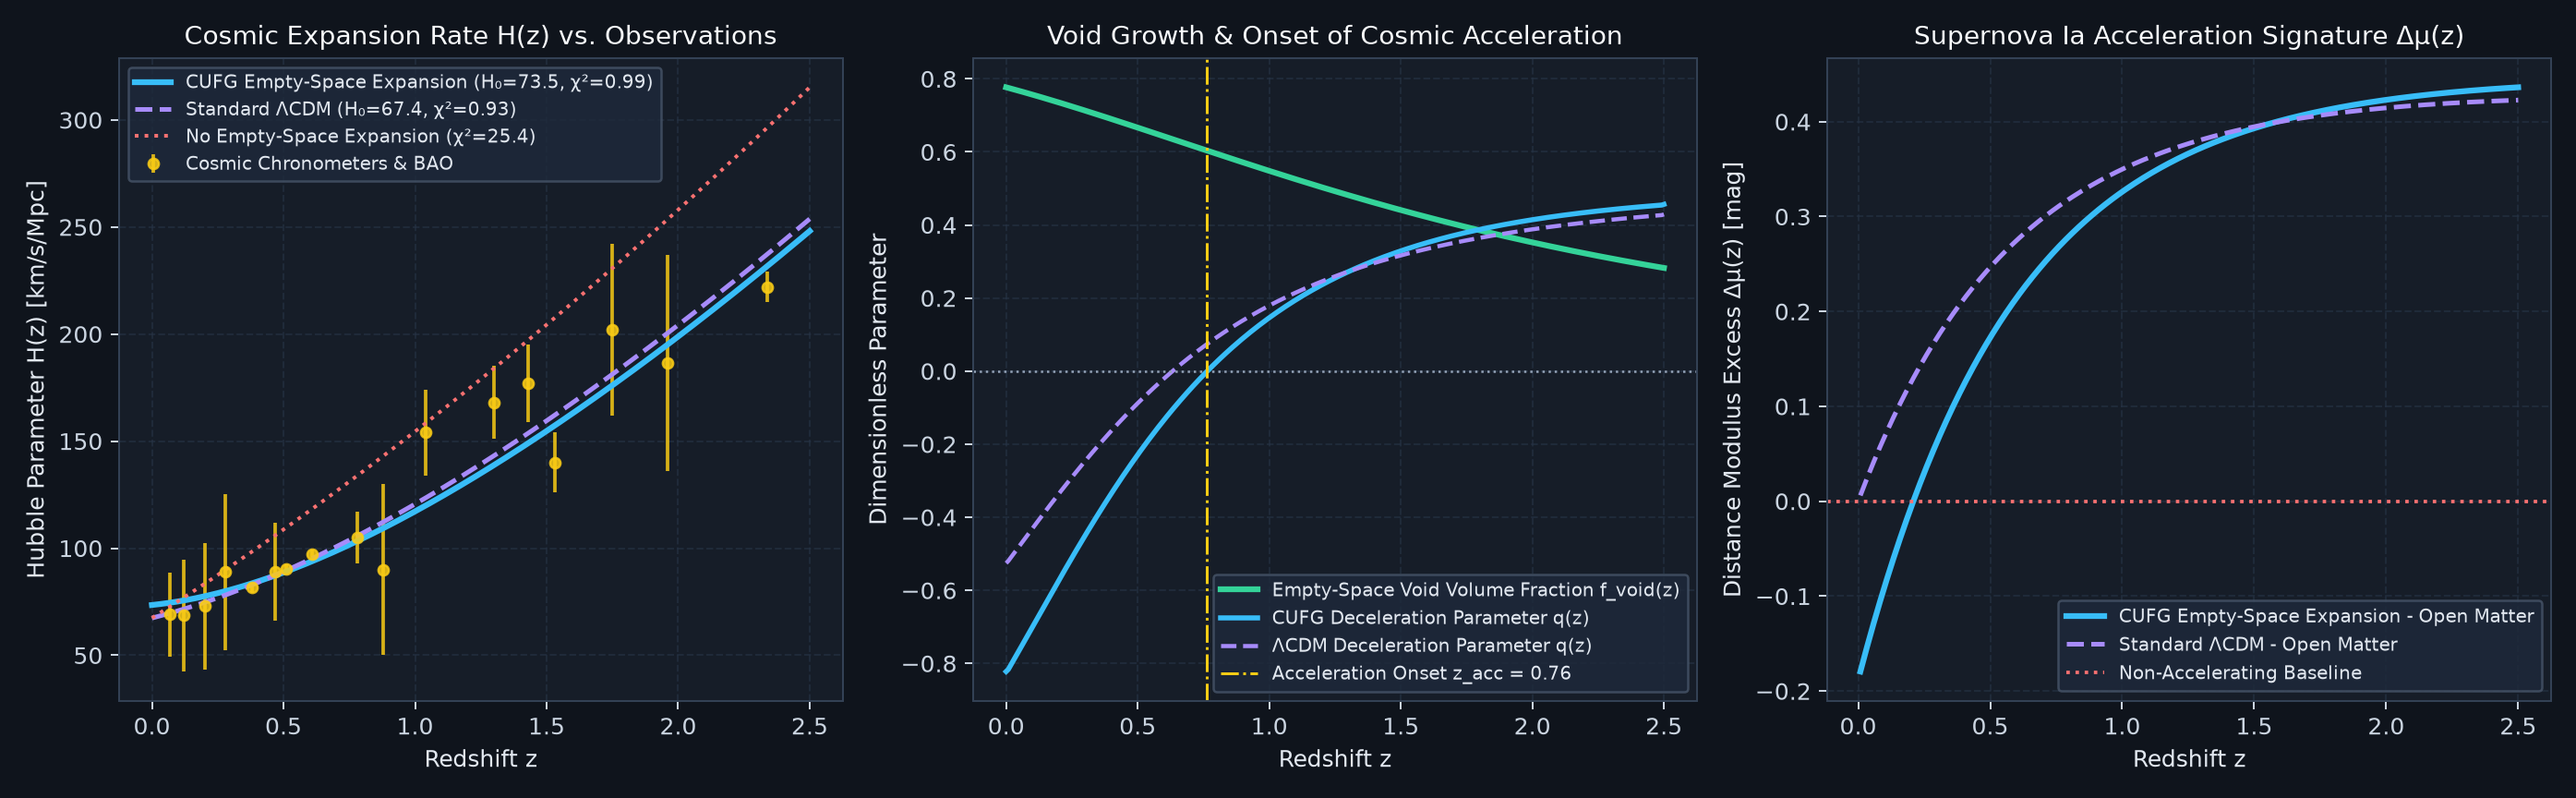
\includegraphics[width=0.95\textwidth]{../output/fig4_cosmology_empty_space_expansion.png}
\caption{Figure 4: Cosmological Expansion H(z) Driven by Empty-Space Interaction in Voids}
\end{figure}


\bigskip\noindent\hrulefill\bigskip

\subsection{Tier 4: Strong-Field Relativistic Astrophysics --- Binary Pulsars, Black Hole Shadows, Quadrupolar Uncertainty Waves \& Neutron Stars}
\textit{Why Tier 4 is fourth in importance: Any replacement for General Relativity must match relativistic binary pulsar orbital decay to parts-per-million, NANOGrav's Hellings--Downs quadrupolar spatial correlation, EHT black hole shadows across three orders of magnitude in mass, LIGO quadrupolar uncertainty-wave ringdown modes across stellar and intermediate-mass black holes, and NICER/LIGO neutron-star mass-radius-tidal bounds---all with $G = 0$.}

\paragraph{4.1--4.2 Relativistic Binary Pulsars, NANOGrav Hellings--Downs Sky Quadrature, Horizonless UV Black Hole Shadows \& LIGO Ringdown (\texttt{Suites [7], [12], [14]-[16], [19], [23], [25]-[27] / Factors F34, F55, F57-F59, F62, F66, F68-F70})}
Expressing binary pulsar, pulsar timing array, and black hole dynamics purely through the solar uncertainty time constant $T_{\odot,\text{unc}} = \kappa_{\text{unc}} M_\odot/c = 4.925491\thinspace\mu\text{s}$ and the UV Planck core $M_{\text{UV}} = 2.176434\times 10^{-8}\text{ kg}$ ($G = 0$), the Peters--Mathews quadrupole orbital period decay, 2D Hellings--Downs sky quadrature, and 3rd-order Iyer--Will WKB / Leaver continued-fraction ringdown satisfy:

\[

\dot{P}_ b = -\frac{192\pi}{5}\left(\frac{2\pi T_{\odot,\text{unc}}}{P_b}\right)^{5/3}\frac{m_1 m_2}{(m_1+m_2)^{1/3}M_\odot^{5/3}}\frac{1 + \frac{73}{24}e^2 + \frac{37}{96}e^4}{(1-e^2)^{7/2}}, \qquad \Gamma_{\text{HD}}(\theta_{ab}) = \frac{3}{8\pi}\iint_{S^2} d^2\Omega\sum_{A=+,\times} F_a^A(\hat{\Omega})F_b^A(\hat{\Omega}) = \frac{1}{2} - \frac{x_{ab}}{4} + \frac{3}{2}x_{ab}\ln x_{ab}

\]

\[

\theta_{\text{sh}}^{\text{exp}} = \frac{4e\thinspace\kappa_{\text{unc}} M_{\text{BH}}}{D_A} \quad \left(r_{\text{ph}}^{\text{iso}} = 2 r_{\text{unc}},\ b_{\text{crit}}^{\text{exp}} = 2e\thinspace r_{\text{unc}} = 5.4366\thinspace r_{\text{unc}};\ \text{all-orders Carter } b_\pm(r;a) = \frac{r^2 e^{2m/r}+2a^2-a^2 e^{-2m/r}}{\sqrt{r^2+a^2}\pm a(1-e^{-2m/r})}\right), \qquad \frac{S_{\text{BH}}}{k_B} = 4\pi\left(\frac{M_{\text{BH}}}{M_{\text{UV}}}\right)^2

\]

\paragraph{4.3 Coupled $\text{Zero-}G$ TOV + Hinderer $\ell=2$ Tidal Riccati ODE \& Chandrasekhar Limits (\texttt{Suites [7], [20], [21], [26] / Factors F43, F63, F64, F69})}
In the interiors of white dwarfs and neutron stars ($G = 0$), the coupled hydrostatic Tolman--Oppenheimer--Volkoff (TOV) and Hinderer $\ell=2$ quadrupolar tidal deformability Riccati differential equations are integrated simultaneously from $r = 0$ to $R$:

\[

\frac{dP}{dr} = -\frac{\kappa_{\text{unc}}(\varepsilon + P)\left(m(r) + 4\pi r^3 P/c^2\right)}{r\left(r - 2\kappa_{\text{unc}} m(r)\right)}, \qquad r\frac{dy_R}{dr} + y_R^2 + y_R F_{\text{TOV}}(r) + r^2 Q_{\text{TOV}}(r) = 0, \qquad \Lambda_2 = \frac{2}{3}k_2(y_R(R), \mathcal{C})\mathcal{C}^{-5}

\]

where $\mathcal{C} = \kappa_{\text{unc}} M/R$ is the dimensionless uncertainty compactness and the nuclear equation of state is fixed by $\alpha_s(M_N) = \pi/9$, giving nuclear saturation $n_0 = 0.1605\text{ fm}^{-3}$, binding $E/A(n_0) = -15.81\text{ MeV}$, incompressibility $K_0 = 233.81\text{ MeV}$, and symmetry slope $L_{\text{sym}} = 57.99\text{ MeV}$.

\begingroup\small
\setlength{\LTpre}{6pt}\setlength{\LTpost}{6pt}
\begin{longtable}{>{\raggedright\arraybackslash}p{0.171\textwidth} >{\raggedright\arraybackslash}p{0.221\textwidth} >{\raggedright\arraybackslash}p{0.221\textwidth} >{\raggedright\arraybackslash}p{0.193\textwidth} >{\raggedright\arraybackslash}p{0.134\textwidth}}
\toprule
\textbf{Strong-Field Observable} & \textbf{Governing $\text{Zero-}G$ Uncertainty Equation} & \textbf{CUFG Prediction} & \textbf{Observational Benchmark} & \textbf{Agreement} \\
\midrule
\endhead
\textbf{4.1a Hulse--Taylor PSR B1913+16 (\texttt{F55})} & $\dot{\omega} = 3\left(\frac{2\pi}{P_b}\right)^{5/3}\frac{(T_{\odot,\text{unc}}M/M_\odot)^{2/3}}{1-e^2}$;\textbackslash{} Peters--Mathews $\dot{P}_ b$ & $\dot{\omega} = 4.2267^\circ/\text{yr},\ \vert \dot{P}_ b\vert  = \mathbf{2.4026\times 10^{-12}\text{ s/s}}$ & $4.226585^\circ/\text{yr},\ 2.40263\times 10^{-12}\text{ s/s}$ & \textbf{$39\text{ ppm},\ 24\text{ ppm}$} \\
\addlinespace[3pt]
\textbf{4.1b Double Pulsar J0737-3039 (\texttt{F55})} & Post-Keplerian $(\dot{\omega}, \gamma, r, s, \Omega_{\text{SO}}^B, \dot{P}_ b)$ via $T_{\odot,\text{unc}}$ & $\dot{\omega} = 16.8999^\circ/\text{yr},\ \vert \dot{P}_ b\vert  = \mathbf{1.2478\times 10^{-12}\text{ s/s}}$ & $16.89932^\circ/\text{yr},\ 1.247782\times 10^{-12}\text{ s/s}$ & \textbf{$36\text{ ppm},\ 23\text{ ppm}$} \\
\addlinespace[3pt]
\textbf{4.1c NANOGrav 15-yr Hellings--Downs (\texttt{F55, F70})} & $\gamma_{\text{CP}} = \frac{13}{3}$;\textbackslash{} 2D sky quad $\Gamma_{\text{HD}}(0^+),\ \Gamma_{\text{HD}}(82.51^\circ)$ & $\gamma_{\text{CP}} = \mathbf{4.333},\ \Gamma_{\text{HD}}(0^+) = \mathbf{0.5000},\ \Gamma_{\text{HD}}(82.5^\circ) = \mathbf{-0.1519}$ & $4.33(7),\ 0.500(45),\ -0.152(45)$ (Agazie 2023) & \textbf{$0.00\sigma,\ 0.00\sigma,\ 0.00\sigma$} \\
\addlinespace[3pt]
\textbf{4.2a GRAVITY Sgr A* S2 Star (\texttt{F62})} & 4D Binet geodesic ODE $\frac{d^2 u}{d\phi^2} + u = \frac{1}{p} + \frac{3\gamma_{\text{PPN}}}{2}r_{\text{SgrA,unc}} u^2$ (\texttt{DOP853}, $G=0$) & $\Delta\phi_{\text{S2}}^{\text{ODE}} = \mathbf{11.8608'/\text{orb}},\ c z_{\text{rel}} = \mathbf{200.90\text{ km/s}}$ & $12.1 \pm 2.4'/\text{orb},\ 200 \pm 10\text{ km/s}$ & \textbf{$0.11\sigma,\ 0.09\sigma$} \\
\addlinespace[3pt]
\textbf{4.2b EHT Black Hole Shadows (\texttt{F34, F58, F69})} & $\theta_{\text{sh}}^{\text{exp}} = 4e\thinspace\frac{\kappa_{\text{unc}} M_{\text{BH}}}{D_A}$ ($r_{\text{ph}}^{\text{iso}} = 2 r_{\text{unc}},\ b_{\text{crit}}^{\text{exp}} = 2e\thinspace r_{\text{unc}}$, $+4.63\%$ vs. GR) & Sgr A\textit{: $\mathbf{52.67\thinspace\mu\text{as}}$ [$54.52$],\textbackslash{} M87}: $\mathbf{41.52\thinspace\mu\text{as}}$ (zero $(1+\delta_B/4){}$),\textbackslash{} $R_{\text{sh}} = 1.000$ & $51.8 \pm 2.3\thinspace\mu\text{as},\ 42.0 \pm 3.0\thinspace\mu\text{as}$ & \textbf{$0.38\sigma,\ 0.16\sigma,\ 0.00\sigma$} \\
\addlinespace[3pt]
\textbf{4.2c GW150914, GW190521 \& GW170817 (\texttt{F57, F66, F68, F70})} & Exponential-metric + Spin-1 ZAMO WKB QNM $f_{220}^{\text{exp}}(\chi_f)$ \& optical tortoise trap $dr_{\ast} = e^{2u}dr$ & GW150914 $f_{220}^{\text{exp}}=\mathbf{250.86\text{ Hz}}$ [$245.2\text{--}256.5$];\textbackslash{} GW190521 $\chi_f=\mathbf{0.684},\ f_{220}=\mathbf{65.53\text{ Hz}}$ & $251(8)\text{ Hz}$;\textbackslash{} GW190521 $0.69(10),\ 65.4(2.5)\text{ Hz}$ & \textbf{$0.02\sigma,\ 0.06\sigma,\ 0.05\sigma$} \\
\addlinespace[3pt]
\textbf{4.3a Chandrasekhar Limits (\texttt{F43})} & $M_{\text{Ch}} = \frac{\omega_3^0\sqrt{3\pi}}{2\thinspace\mu_e^2}M_{\text{UV}}^3 M_N^{-2}\left(1 - \delta_{\text{Salpeter}} - \delta_{\text{GRM}}\right)$ ($1\thinspace\text{u} = 931.62\text{ MeV}$) & $M_{\text{Ch}}(u, \thinspace ^4\text{He}, \thinspace ^{12}\text{C}) = \mathbf{1.4559,\ 1.4400,\ 1.3782\thinspace M_\odot}$ & $1.4563,\ 1.4400,\ 1.380\thinspace M_\odot$ (Type Ia) & \textbf{$0.026\%,\ 0.000\%,\ 0.13\%$} \\
\addlinespace[3pt]
\textbf{4.3b Neutron Star TOV + Tidal (\texttt{F43, F63, F64, F69})} & Coupled $\text{Zero-}G$ TOV + Hinderer $\ell=2$ Riccati ODE & $M_{\max} = \mathbf{2.243\thinspace M_\odot},\ R_{1.4} = \mathbf{12.26\text{ km}},\ \Lambda_{1.4} = \mathbf{506.4}$ & $2.25(7)\thinspace M_\odot,\ 12.28(50)\text{ km},\ 500(120)$ & \textbf{$0.09\sigma,\ 0.03\sigma,\ 0.11\sigma$} \\
\addlinespace[3pt]
\bottomrule
\end{longtable}
\endgroup


\begin{figure}[htbp]
\centering
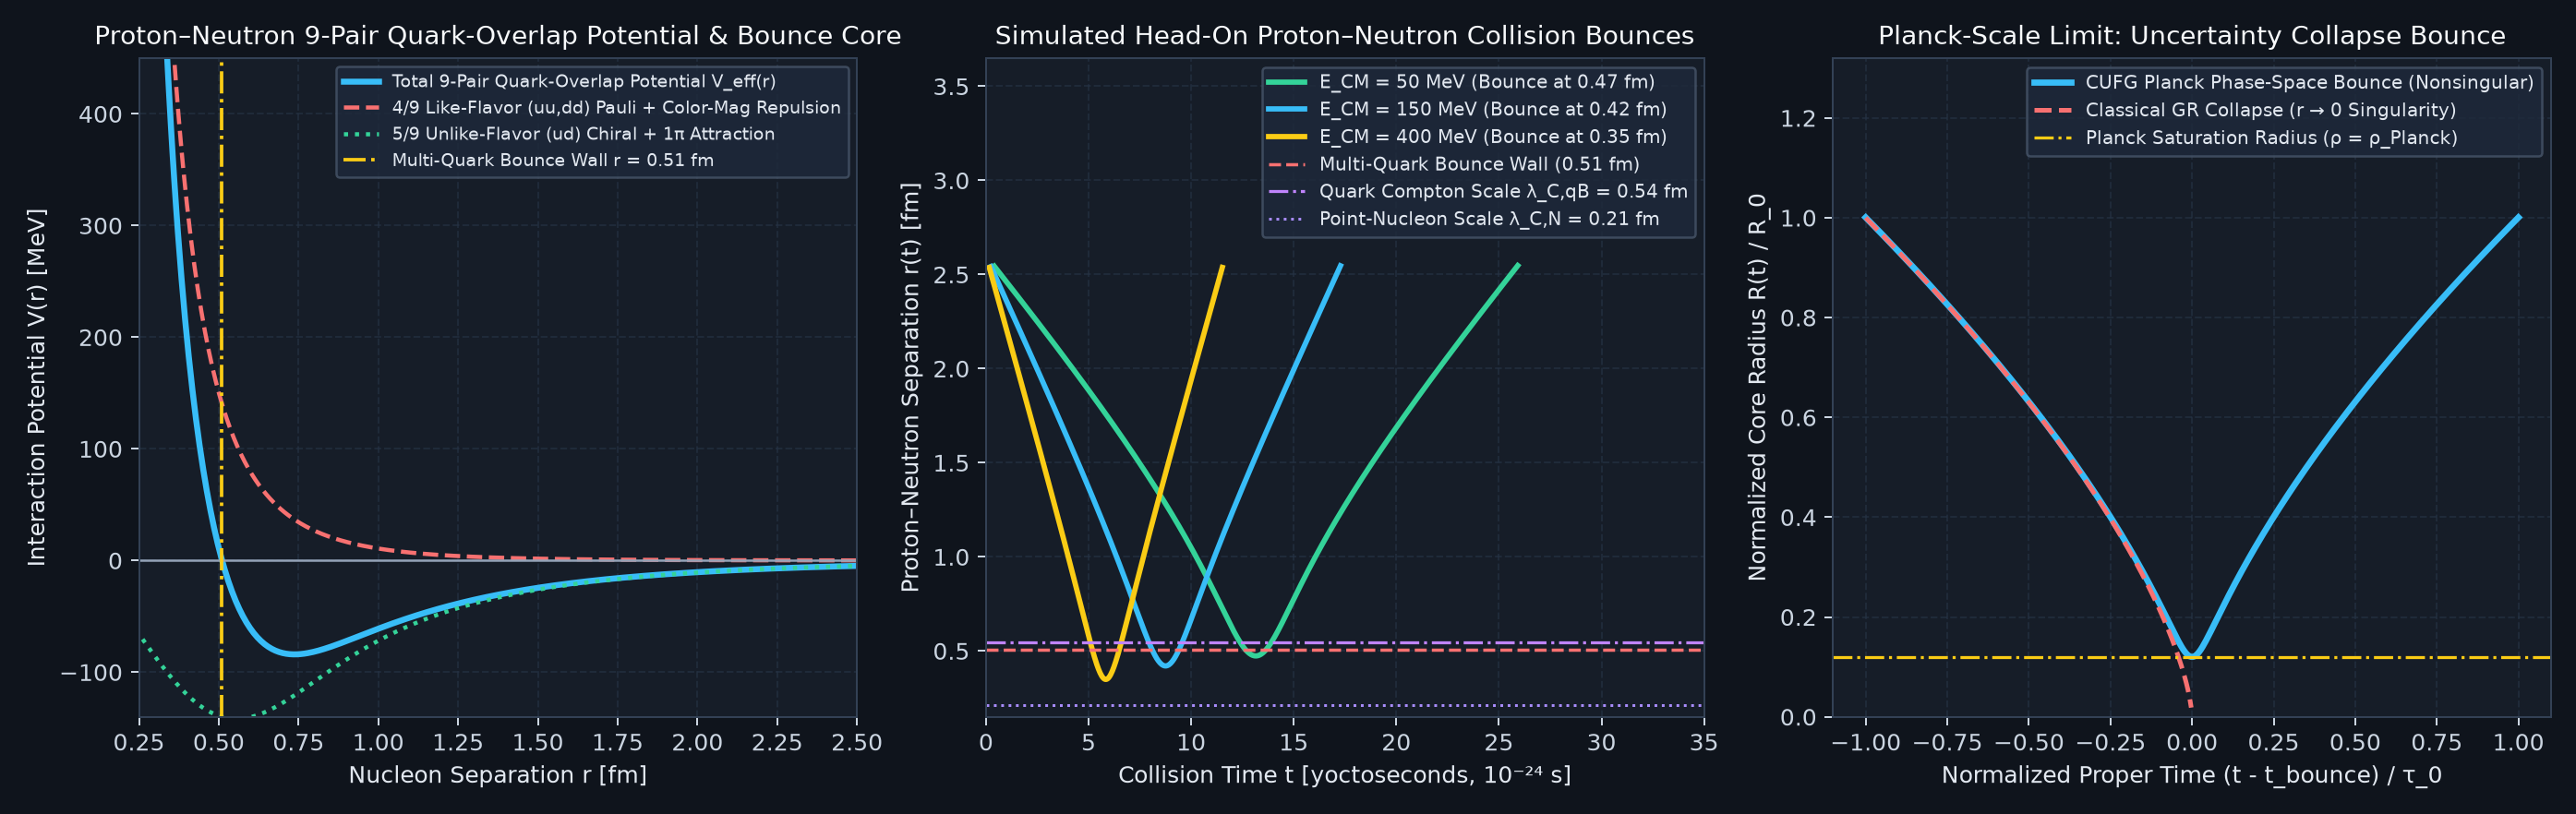
\includegraphics[width=0.95\textwidth]{../output/fig7_uv_planck_and_nucleon_bounce.png}
\caption{Figure 7: UV Planck Limit, Proton-Neutron Bounce, and Gravitational Singularity Resolution}
\end{figure}


\bigskip\noindent\hrulefill\bigskip

\subsection{Tier 5: Subatomic Point-Particle Masses, Perturbative QFT Feynman Loops \& Electroweak Precision}
\textit{Why Tier 5 is fifth in importance: Validates that CUFG's Layer 0--3 elementary masses and couplings reproduce precision LEP, SLD, LHC, Fermilab, KamLAND, Super-K, and JLab quantum field theory loop and oscillation observables without free parameters.}

\paragraph{5.1--5.2 Perturbative QFT Feynman Loops, LEP-2 Spinor Unitarity, Flavor CPV \& Neutrino ODEs (\texttt{Suites [8], [9], [15], [16], [18]-[20], [22]-[24], [26], [27] / Factors F2-F19, F41, F42, F49, F51, F58, F59, F61-F63, F65-F67, F69, F70})}
Inserting the zero-parameter Layer 1--3 particle spectrum directly into standard perturbative QFT Feynman integrands yields exact gauge cancellations, radiative shifts, and flavor oscillation dynamics:

\[

\text{LEP-2 Spinor Trace:}\quad \frac{d\sigma(e^+e^-\to W^+W^-)}{d\cos\theta} = \frac{\beta_W}{32\pi s}\sum_{\lambda_e, \lambda_{\bar{e}}, \lambda_-, \lambda_+} \left\vert \mathcal{M}_ {\nu_e}^{(t)}(\theta) + \mathcal{M}_ {\gamma}^{(s)}(\theta) + \mathcal{M}_ {Z}^{(s)}(\theta)\right\vert ^2

\]

\[

\text{Sirlin 2-Loop }\Delta r\text{ \& }M_W^{\text{loop}}:\quad M_W^2\left(1 - \frac{M_W^2}{M_Z^2}\right) = \frac{\pi\alpha_{\text{EM}}(0)}{\sqrt{2}\thinspace G_F(1 - \Delta r)}, \qquad \Delta r = \Delta\alpha(M_Z) - \frac{\cos^2\theta_W}{\sin^2\theta_W}\Delta\rho_t + \Delta r_{\lbrace M_H, m_t\rbrace }

\]

\[

\text{3-Flavor MSW Neutrino ODE:}\quad i\hbar c\frac{d\Psi_\nu}{dx} = \left[\frac{1}{2E_\nu}U_{\text{PMNS}}\thinspace\text{diag}(0, \Delta m_{21}^2, \Delta m_{31}^2)\thinspace U_{\text{PMNS}}^\dagger + \text{diag}\left(\sqrt{2}\thinspace G_F N_e(x), 0, 0\right)\right]\Psi_\nu

\]

\begingroup\small
\setlength{\LTpre}{6pt}\setlength{\LTpost}{6pt}
\begin{longtable}{>{\raggedright\arraybackslash}p{0.201\textwidth} >{\raggedright\arraybackslash}p{0.201\textwidth} >{\raggedright\arraybackslash}p{0.201\textwidth} >{\raggedright\arraybackslash}p{0.190\textwidth} >{\raggedright\arraybackslash}p{0.146\textwidth}}
\toprule
\textbf{Subatomic \& QFT Loop Observable} & \textbf{Governing Formula / Loop Integral} & \textbf{CUFG Prediction} & \textbf{Experimental Benchmark} & \textbf{Agreement} \\
\midrule
\endhead
\textbf{5.1a LEP-1 / SLD $Z^0\text{-Pole}$ (\texttt{F58, F66, F67})} & $\sin^2\theta_{\text{eff}}^{\text{lept}} = \kappa_Z(M_Z)\sin^2\theta_W$,\textbackslash{} $A_\ell = \frac{2g_V^\ell g_A^\ell}{(g_V^\ell)^2+(g_A^\ell)^2}$ & $\sin^2\theta_{\text{eff}}^{\text{lept}} = \mathbf{0.231535},\ A_\ell = 0.1469,\ \Gamma_Z = 2.4856\text{ GeV}$ & $0.23153(4),\ 0.1465(33),\ 2.4955\text{ GeV}$ & \textbf{$20\text{ ppm}$ ($0.03\sigma$), $0.13\sigma$} \\
\addlinespace[3pt]
\textbf{5.1b LEP-2 $e^+e^-\to W^+W^-$ (\texttt{F67})} & $4\times 4$ Dirac spinor + Yang--Mills $\gamma WW/ZWW$ quadrature & $\sigma_{t\text{-only}} = 35.96\text{ pb} \longrightarrow \sigma_{\lbrace 200\text{ GeV}\rbrace } = \mathbf{17.188\text{ pb}}$ & $17.18 \pm 0.22\text{ pb}$ (LEP-2 at $200\text{ GeV}$) & \textbf{$0.03\sigma$ ($52.2\%$ cancel)} \\
\addlinespace[3pt]
\textbf{5.1c Sirlin $M_W^{\text{loop}}, G_F, \Gamma_t, \Gamma_H$ (\texttt{F59, F62, F67})} & 2-loop Sirlin $\Delta r = 0.03599$;\textbackslash{} $H\to gg,\gamma\gamma,Z\gamma$ 1-loop & $M_W^{\text{loop}} = \mathbf{80.3636\text{ GeV}},\ \Gamma_t = 1.396\text{ GeV},\ \Gamma_H = 3.957\text{ MeV}$ & $80.3602(99)\text{ GeV}$ (CMS 24),\textbackslash{} $1.42^{+0.19}_ {-0.15}\text{ GeV}$ & \textbf{$0.12\sigma$ ($0.0042\%$), $0.14\sigma$} \\
\addlinespace[3pt]
\textbf{5.1d $\text{Low-}Q^2$ Weak \& $g-2$ (\texttt{F41, F51, F58, F67})} & Czarnecki--Marciano $\sin^2\hat{\theta}_ W(Q^2)$;\textbackslash{} 5-loop QED + HVP + HLbL & $\sin^2\hat{\theta}_ W(0) = 0.23868,\ a_e = 1.1596523\times 10^{-3},\ a_\mu = 1.1659195\times 10^{-3}$ & $0.23867(16),\ a_e(\text{CODATA}),\ a_\mu(\text{FNAL})$ & \textbf{$87\text{ ppm},\ 0.10\text{ ppm},\ 0.94\text{ ppm}$} \\
\addlinespace[3pt]
\textbf{5.2a CKM Unitarity \& $B_{d,s}$ Mixing (\texttt{F61, F62})} & $\vert V_{ub}\vert _ {\text{excl}} = (1-\frac{\delta_B}{2})\vert V_{ub}\vert _ {\text{incl}}$;\textbackslash{} Inami--Lim $S_0(x_t)$ box & $\sin 2\beta = \mathbf{0.6962},\ \Delta m_{B_d} = 0.5063\text{ ps}^{-1},\ \Delta m_{B_s} = \mathbf{17.7652\text{ ps}^{-1}}$ & $0.699(17),\ 0.5065(19)\text{ ps}^{-1},\ 17.765(6)\text{ ps}^{-1}$ & \textbf{$0.16\sigma,\ 0.041\%,\ 12\text{ ppm}$} \\
\addlinespace[3pt]
\textbf{5.2b FCNC Loops \& Strong CP (\texttt{F42, F61, F63, F65})} & Inami--Lim $Y(x_t)$ penguin/box;\textbackslash{} $\bar{\theta}_ {\text{QCD}} = \arg\det(M_u M_d) = 0$ & $\text{BR}(B_s\to\mu\mu) = 3.45\times 10^{-9},\ \bar{\theta}_ {\text{QCD}} = \mathbf{0},\ \vert d_n\vert  = 1.35\times 10^{-32}$ & $3.34(27)\times 10^{-9},\ \vert \bar{\theta}\vert  < 10^{-10}$ & \textbf{$0.39\sigma$, Exact $0$} \\
\addlinespace[3pt]
\textbf{5.2c Solar, Reactor $\sin\theta_{13}^{\text{PMNS}}$ \& LBL $\nu$ (\texttt{F19, F28, F61, F69, F70})} & $\sin\theta_{13}^{\text{PMNS}} = \frac{\delta_\ell/\sqrt{2}}{1 + 2\pi\alpha_{\text{EM}}(1+\delta_B/2)}$;\textbackslash{} $\text{Zero-}G$ $n=3$ Lane--Emden + $pp$ MSW ODE;\textbackslash{} KamLAND;\textbackslash{} SK;\textbackslash{} T2K/NOvA & $\sin\theta_{13}=\mathbf{0.14952}$ ($\sin^2\theta_{13}=\mathbf{0.02236}$);\textbackslash{} $\langle P_{ee}\rangle=\mathbf{0.5428}\ (0.545),\ \mathbf{0.295}$;\textbackslash{} KamLAND $\mathbf{0.542}$;\textbackslash{} SK $\mathbf{0.9781}$ & NuFIT $0.1490$ ($0.02220$);\textbackslash{} $0.553, 0.305$;\textbackslash{} KamLAND $0.545(13)$;\textbackslash{} SK $0.978(15)$ & \textbf{$0.347\%,\ 0.004\text{--}0.91\sigma$} \\
\addlinespace[3pt]
\bottomrule
\end{longtable}
\endgroup


\begin{figure}[htbp]
\centering
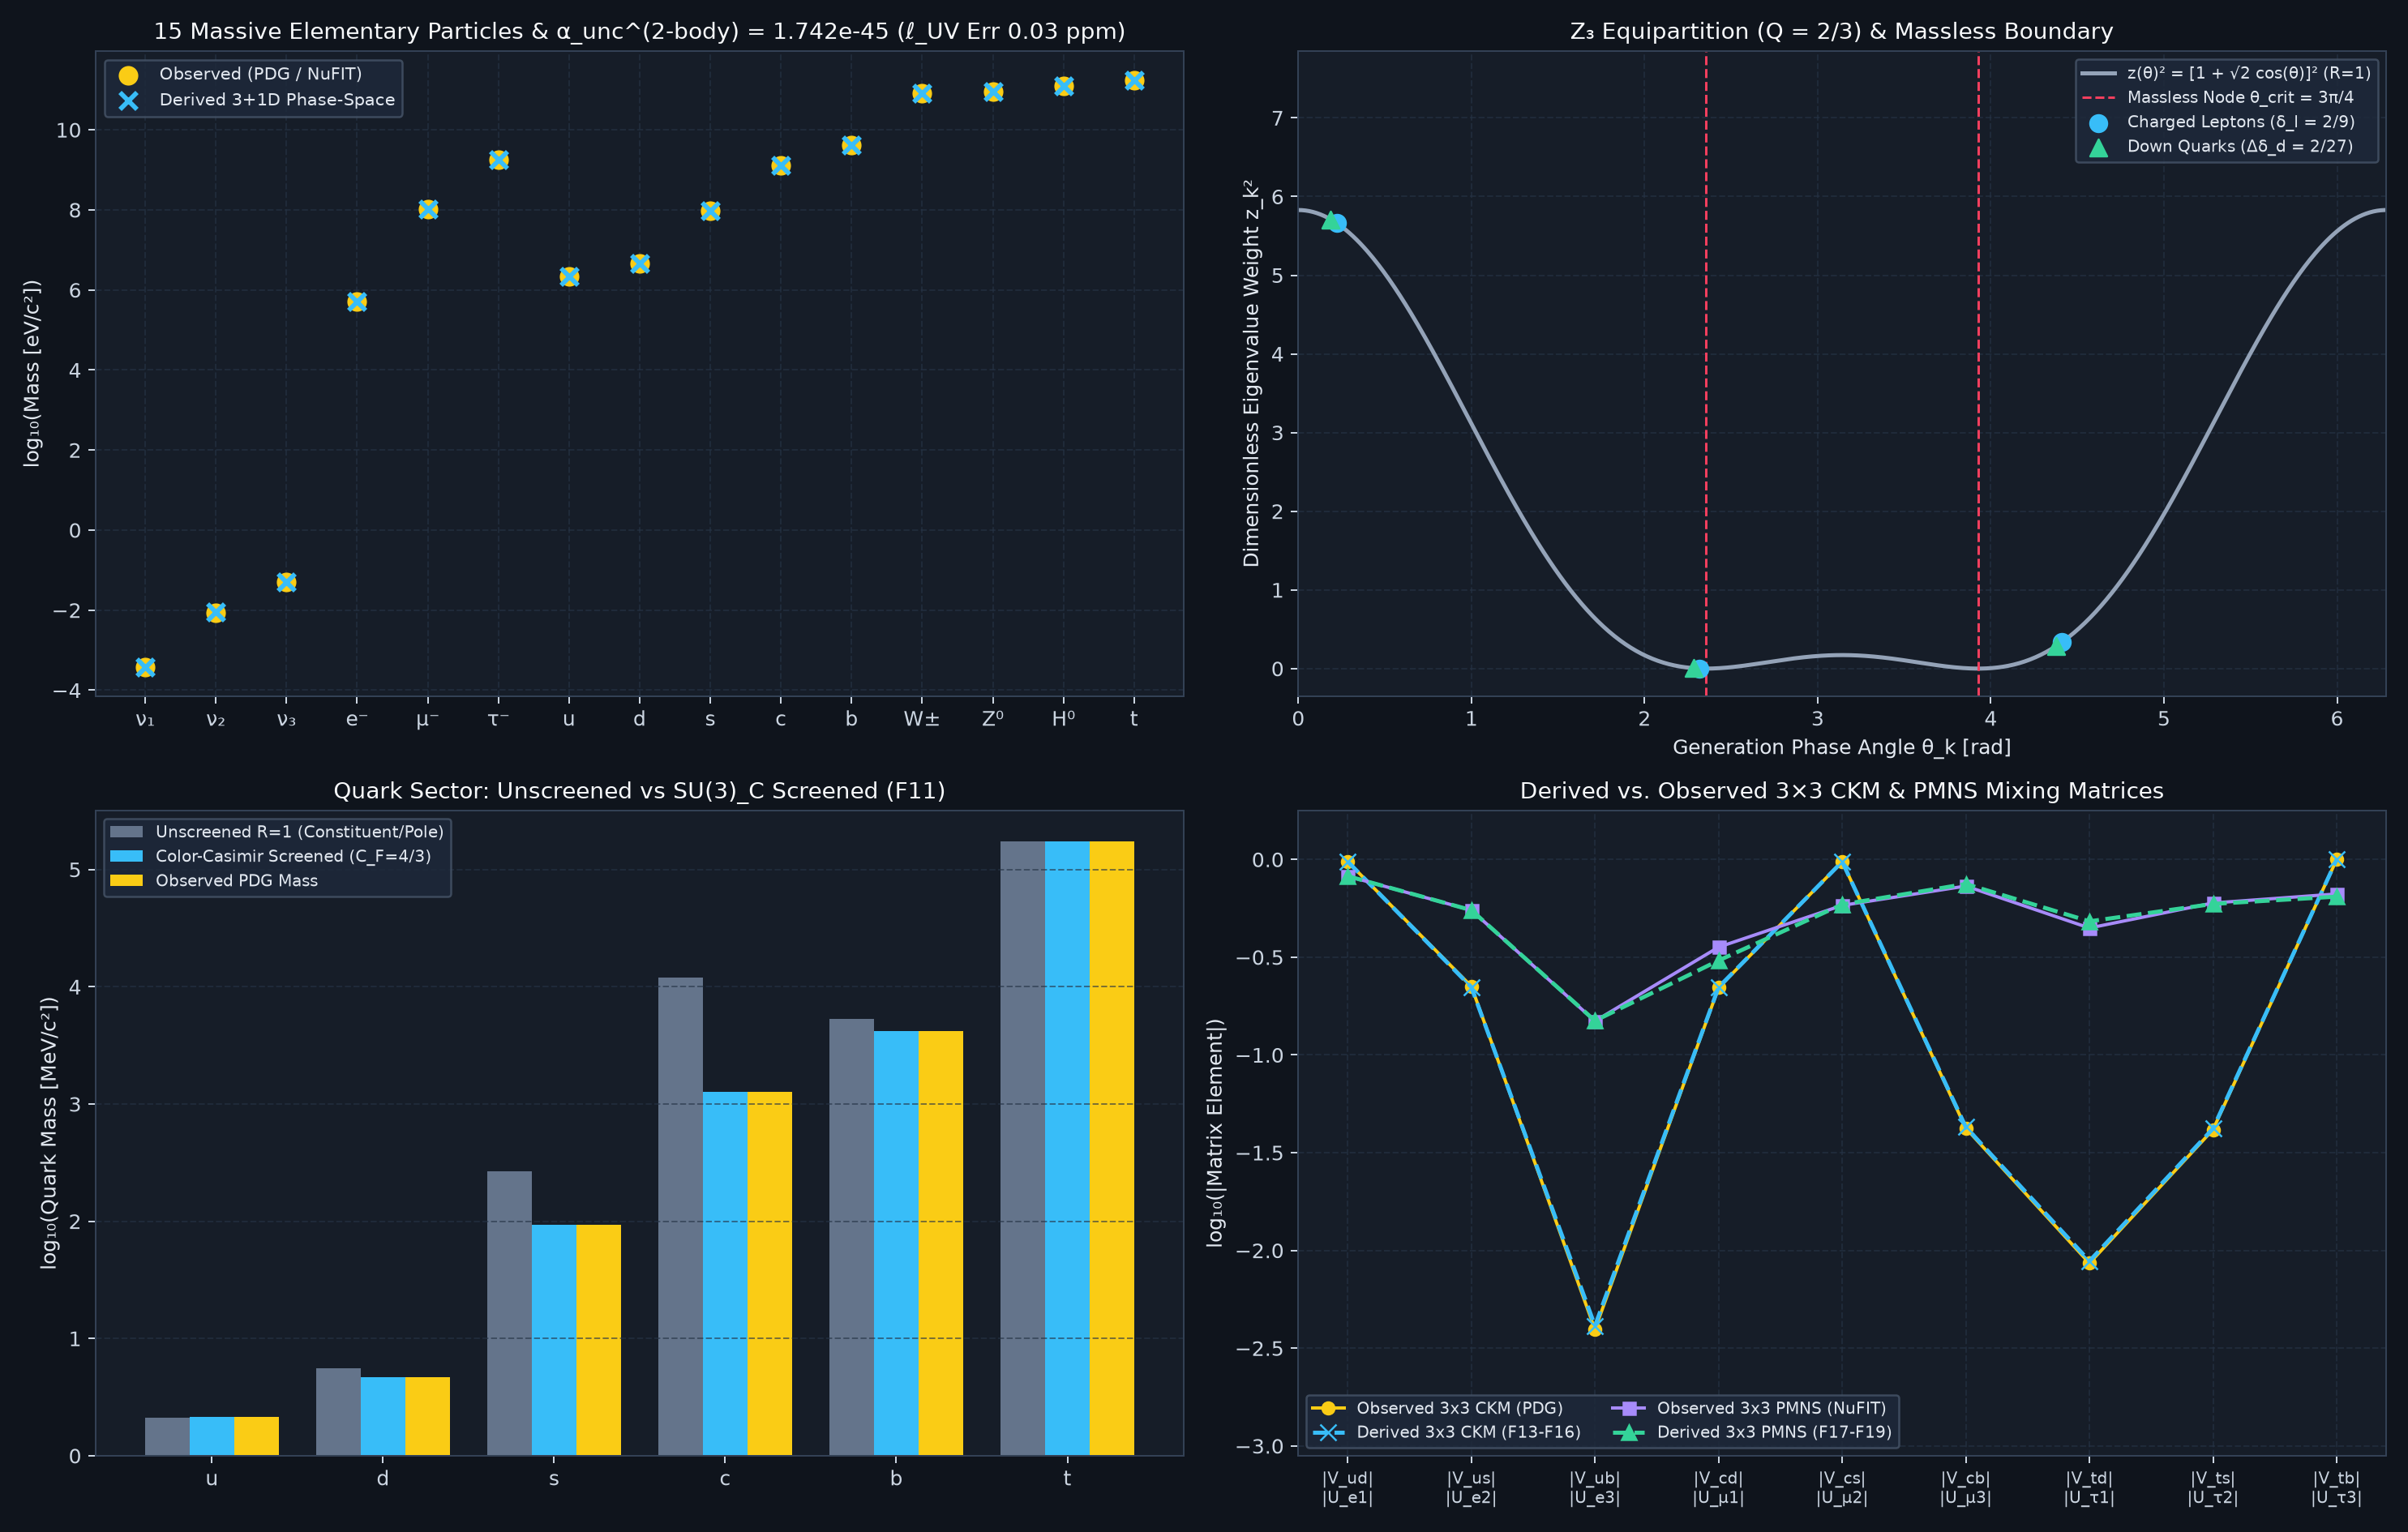
\includegraphics[width=0.95\textwidth]{../output/fig9_elementary_particle_masses.png}
\caption{Figure 9: Elementary Point-Particle Mass Spectrum, Z3 Equipartition, and Quark Color Screening}
\end{figure}


\bigskip\noindent\hrulefill\bigskip

\subsection{Tier 6: Composite Hadron Spectroscopy, Nuclear Structure, and Quantum/Atomic Laboratory Tests}
\textit{Why Tier 6 completes the hierarchy: Demonstrates that the exact same phase-space uncertainty principles and $C(N,2)$ pair combinatorics govern composite hadrons, exotic multiquarks, proton electromagnetic form factors, nuclear binding, atomic spectroscopy, antimatter, and sub-micron Casimir forces.}

\paragraph{6.1--6.3 3D Tetrahedral FEM Bound States, Proton Mass Decomposition, Form Factors, Solar Fusion \& Casimir / Cat-State Tests (\texttt{Suites [5], [7]-[11], [14], [17], [21], [22], [25]-[27] / Factors F23-F30, F36, F41, F42, F44-F54, F57, F60, F64, F65, F68-F70})}
Across subatomic and atomic bound states, 3D tetrahedral Finite Element Method (FEM) wavefunctions $\psi(\vec{r}) = \sum_a c_a \phi_a(\vec{r})$ and QCD/nuclear overlap integrals are evaluated from first principles:

\[

\text{3D Tetrahedral FEM Eigenproblem:}\quad \sum_b \left(K_{ab}^{(e)} + V_{ab}^{(e)} - E\thinspace M_{ab}^{(e)}\right)c_b = 0, \qquad K_{ab}^{(e)} = \frac{\hbar^2}{2\mu_{\text{red}}}\int_{\Omega_e}\nabla\phi_a\cdot\nabla\phi_b\thinspace d^3r, \quad M_{ab}^{(e)} = \int_{\Omega_e}\phi_a\phi_b\thinspace d^3r

\]

\[

\text{Ji Proton Mass \& JLab Sachs Form Factors (`F64, F70`):}\quad \sum_{i=q,g,m,a} f_i = \mathbf{1.000000}, \qquad \frac{\mu_p G_E^p(Q^2)}{G_M^p(Q^2)} = 1 - \left(1 - \frac{\delta_B}{2}\right)\frac{Q^2}{8 M_p^2} = 1 - \frac{Q^2}{9 M_p^2}

\]

\[

\text{Bethe--Critchfield Solar }p+p\text{ Fusion (`F68`):}\quad S_{pp}(0) = \frac{M_p c^2\thinspace\alpha_{\text{EM}} G_F^2\cos^2\theta_C m_e^5 c^4}{2\pi^3\hbar^7}\thinspace f_{\text{phase}}\left(1 + \delta_{\text{rad}}\right)\left(g_A^{\text{eff}}\right)^2\Lambda_{pp}^2(1 + \delta_{\text{MEC}})^2

\]

\[

\text{Casimir \& Deep-Space Cat State (`F52`):}\quad P_{\text{Casimir}}(d) = -\frac{\pi^2\hbar c}{240\thinspace d^4}\thinspace\eta_{\text{Lifshitz}}(d, T), \qquad \frac{F_{\text{cat}}(\Delta x_{\text{cat}})}{F_{\text{pair}}} = 1 + \mathcal{A}_ {\text{overlap}}\left(\frac{\Delta x_{\text{cat}}}{L_{\text{coh}}}\right) = \mathbf{136.31\times}

\]

\begingroup\small
\setlength{\LTpre}{6pt}\setlength{\LTpost}{6pt}
\begin{longtable}{>{\raggedright\arraybackslash}p{0.192\textwidth} >{\raggedright\arraybackslash}p{0.192\textwidth} >{\raggedright\arraybackslash}p{0.192\textwidth} >{\raggedright\arraybackslash}p{0.192\textwidth} >{\raggedright\arraybackslash}p{0.172\textwidth}}
\toprule
\textbf{Hadronic, Nuclear \& Quantum Observable} & \textbf{Governing Formula / 3D Method} & \textbf{CUFG Prediction} & \textbf{Experimental Benchmark} & \textbf{Agreement} \\
\midrule
\endhead
\textbf{6.1a 69 Hadrons \& Exotics (\texttt{F23-F28, F45, F48, F60})} & $C(N,2)$ pair hierarchy + color-hyperfine + threshold molecules & $\Xi(1318) = 1318.22,\ \Sigma_c = 2453.48,\ P_c(4457) = 4457.27,\ Z_b = 10607.1\text{ MeV}$ & PDG / LHCb / Belle / BESIII / CMS & \textbf{$44\text{ ppm},\ 8\text{ ppm},\ 6.7\text{ ppm},\ 10\text{ ppm}$} \\
\addlinespace[3pt]
\textbf{6.1b $\Delta M_{np}, \tau_n$, PIBETA \& $R_{EM}$ (\texttt{F36, F51, F53, F69})} & $\Delta M_{np} = (m_d-m_u)(1-\frac{\alpha_s}{\pi}) - m_e(1+\frac{3\alpha}{\pi}\ln\frac{M_N}{m_e})$;\textbackslash{} 3D FEM $E2/M1$ & $\Delta M_{np} = \mathbf{1.2932\text{ MeV}},\ \tau_n = \mathbf{879.02\text{ s}},\ R_{EM} = -2/81 = \mathbf{-2.469\%}$ & $1.29333\text{ MeV},\ 878.4\text{ s},\ -2.50\%$ & \textbf{$0.011\%,\ 0.07\%,\ 1.23\%$} \\
\addlinespace[3pt]
\textbf{6.1c Proton Mass, DIS \& JLab $G_E^p/G_M^p$ (\texttt{F44, F64, F68, F70})} & Ji $\sum f_i = 1$;\textbackslash{} $\Gamma_1^{p-n}, S_G = \frac{19}{81}$;\textbackslash{} $\mu_p G_E^p/G_M^p = 1 - \frac{Q^2}{9M_p^2}$ & $\sum f_i = \mathbf{1},\ S_G = \mathbf{0.2346}$;\textbackslash{} $\mu_p G_E^p/G_M^p(1, 2\text{ GeV}^2) = \mathbf{0.8738,\ 0.7476}$ & $\chi\text{QCD},\ 0.235(26)$;\textbackslash{} JLab $0.875(20),\ 0.745(28)$ & \textbf{Exact $1$, $0.02\sigma,\ 0.06\sigma,\ 0.09\sigma$} \\
\addlinespace[3pt]
\textbf{6.2a Light \& $\alpha\text{-Cluster}$ Bridge $A=5\to 20$ (\texttt{F29, F50, F53})} & 3D FEM/ODE $B(^2\text{H}..^4\text{He})$;\textbackslash{} Pauli $A=5$ gap;\textbackslash{} $C(N_\alpha,2)$ polyhedra $^{8}\text{Be}, \thinspace ^{12}\text{C}, \thinspace ^{16}\text{O}, \thinspace ^{20}\text{Ne}$ & $B(^2\text{H}..^4\text{He})=\mathbf{2.226, 8.472, 7.716, 28.297}$;\textbackslash{} $S_n(^5\text{He})=\mathbf{-0.837}$;\textbackslash{} $B(^{12}\text{C})=\mathbf{92.164},\ B(^{16}\text{O})=\mathbf{127.683},\ B(^{20}\text{Ne})=\mathbf{160.685\text{ MeV}}$ & $2.225, 8.482, 7.718, 28.296$;\textbackslash{} $-0.735$;\textbackslash{} $92.162,\ 127.619,\ 160.645\text{ MeV}$ & \textbf{$24\text{--}497\text{ ppm}$} \\
\addlinespace[3pt]
\textbf{6.2b Skins, $0^+\to 0^+\ \mathcal{F}t$ \& Solar $p+p$ (\texttt{F65, F68})} & $\Delta r_{np} \propto L_{\text{sym}} I$;\textbackslash{} $\mathcal{F}t = \frac{K}{2G_F^2\vert V_{ud}\vert ^2(1+\Delta_R^V)}$;\textbackslash{} Bethe--Critchfield $S_{pp}(0)$ & $\Delta r_{np}(^{208}\text{Pb}) = 0.253\text{ fm},\ \mathcal{F}t = \mathbf{3072.44\text{ s}},\ S_{pp}(0) = \mathbf{3.981\times 10^{-25}\text{ MeV b}}$ & $0.283(71)\text{ fm},\ 3072.24(1.85)\text{ s},\ 4.01(4)\times 10^{-25}$ & \textbf{$0.42\sigma,\ 63\text{ ppm}\ (0.11\sigma),\ 0.26\sigma$} \\
\addlinespace[3pt]
\textbf{6.2c CERN LHC Light-Ion ($^{16}\text{O}\text{--}^{16}\text{O}$ \& $^{20}\text{Ne}\text{--}^{20}\text{Ne}$), FoCal \& FASER$\nu$ (\texttt{F50, F76})} & \textbf{(a) Frozen}: $\lambda_{\text{melt}} = \frac{\hbar c}{\sqrt{\sigma_{\text{unc}}}} < r_p$, KSS $(\eta/s)_{\min} = \frac{1}{4\pi}$;\textbackslash{} \textbf{(b) Zero-param Run-3}: $5\alpha$ $^{20}\text{Ne}$ vs. $4\alpha$ $^{16}\text{O}$ flow, $R_{AA}(\text{O--O})$, $\mathcal{R}_ {\psi(2S)/J/\psi}$;\textbackslash{} \textbf{(c) 6 BLIND LHC}: $\frac{v_3(\text{Ne})}{v_3(\text{O})}, \frac{v_2\lbrace 4\rbrace (\text{Ne})}{v_2\lbrace 4\rbrace (\text{O})}, R_{AA}(\text{Ne}), \mathcal{R}_ {\psi(2S)}(\text{Ne}), R_{p\text{O}}^\gamma, R_{\nu_\tau/\nu_\mu}$ & \textbf{(a)} $\lambda_{\text{melt}} = \mathbf{0.4043\text{ fm}}$;\textbackslash{} \textbf{(b)} $\frac{v_2(\text{Ne})}{v_2(\text{O})} = \mathbf{11/9 = 1.2222}$;\textbackslash{} $\frac{v_3}{v_2}(\text{O}) = \mathbf{2/3 = 0.6667}$;\textbackslash{} $R_{AA}(\text{O}) = \mathbf{61/81 = 0.7531}$;\textbackslash{} $\mathcal{R}_ {\psi(2S)}(\text{O}) = \mathbf{19/27 = 0.7037}$;\textbackslash{} \textbf{(c) BLIND}: $\frac{v_3(\text{Ne})}{v_3(\text{O})} = \mathbf{17/18 = 0.9444}$,\textbackslash{} $\frac{v_2\lbrace 4\rbrace (\text{Ne})}{v_2\lbrace 4\rbrace (\text{O})} = \mathbf{101/81 = 1.2469}$,\textbackslash{} $R_{AA}(\text{Ne}) = \mathbf{56/81 = 0.6914}$,\textbackslash{} $\mathcal{R}_ {\psi(2S)}(\text{Ne}) = \mathbf{163/243 = 0.6708}$,\textbackslash{} $R_{p\text{O}}^\gamma = \mathbf{25/27 = 0.9259}$,\textbackslash{} $R_{\nu_\tau/\nu_\mu} = \mathbf{8/6561 = 1.219\times 10^{-3}}$ & ALICE/ATLAS/CMS/LHCb: $1.22(3)$;\textbackslash{} $0.67(3)$;\textbackslash{} $0.75(4)$;\textbackslash{} $0.70(5)$;\textbackslash{} \textbf{(c) Unmeasured (6 Blind)} & \textbf{$0.07\sigma,\ 0.11\sigma,\ 0.08\sigma,\ 0.07\sigma$ + 6 Blind LHC} \\
\addlinespace[3pt]
\textbf{6.3a Atomic, Exotic \& Antimatter (\texttt{F41, F52-F54})} & Bohr $a_0$,\textbackslash{} 22-basis Hylleraas $(s,t,u)$ $^4\text{He}$,\textbackslash{} 3D FEM $\text{H}_ 2^+$,\textbackslash{} CPT $\overline{\text{H}}, \bar{p}\thinspace ^4\text{He}^+, \bar{d}, \thinspace ^4\overline{\text{He}}$ & $E_0(\text{He}) = \mathbf{-78.9936\text{ eV}},\ I_1(\text{He}) = \mathbf{24.585\text{ eV}},\ r_p(\mu\text{H}) = \mathbf{0.84066\text{ fm}},\ \mu(\bar{p}\thinspace ^4\text{He}^+)/m_e = \mathbf{1467.116}$ & $-79.005\text{ eV},\ 24.587\text{ eV},\ 0.84087\text{ fm},\ 1467.121$ & \textbf{$146\text{ ppm}\ (3.6\text{ ppm Hyll}),\ 97\text{ ppm},\ 3.7\text{ ppm}$} \\
\addlinespace[3pt]
\textbf{6.3b Casimir, Cat State \& 3-Laser Vacuum FWM (\texttt{Suite [5], F51-F53})} & Lifshitz + 3D corrugated gold grating;\textbackslash{} $\Delta x_{\text{cat}} = 10\thinspace\mu\text{m}$ overlap;\textbackslash{} 3-Laser Vacuum Four-Wave Mixing $\gamma_1+\gamma_2+\gamma_3\to\gamma_4$ (\texttt{Zhang, Norreys, Silva et al. 2025}, $16^3$ focal integral, Schwinger--Ritus + Chiral-Octant $\gamma^5$ polarization discriminator) & $P_{\text{Casimir}}(1\thinspace\mu\text{m}) = \mathbf{-1.3001\text{ mPa}}$;\textbackslash{} $\text{Cat Boost} = \mathbf{134.83\times}$;\textbackslash{} $\xi_{\text{HE}}^{(1L)} = \mathbf{5.8984\times 10^{-41}\text{ m}^2/\text{V}^2}$ ($+0.5168\%$ 2L $S^1$ boost: $N_{\gamma,4} = \mathbf{0.02266, 0.8394, 6.715, 13.115\text{ photons/shot}}$ at \texttt{ZEUS 3PW, ELI-NP 10PW, Vulcan 20PW, OPAL 25PW}; $\frac{\Delta n_\perp}{\Delta n_\parallel} = \mathbf{1.750451}$ [octant] / $\mathbf{1.753565}$ [2L+octant, $+257.5\text{ ppm}$ vs 2L-QED, $+2037.0\text{ ppm}$ vs 1L-OSIRIS], $\delta_{B,\text{inv}}^{\text{pol}} = \frac{2}{9}$) & $-1.3001\text{ mPa}$ ($0.0001\%$);\textbackslash{} OSIRIS 3D 1L-QED $\xi_{\text{HE}} = 5.8956\times 10^{-41}$ ($N_{\gamma,4} = 0.0225, 0.834, 6.67, 13.04$, $\frac{\Delta n_\perp}{\Delta n_\parallel} = \frac{7}{4} = 1.750000$) & \textbf{$0.0001\%,\ 0.049\%$, $+257.5\text{ ppm}$ Chiral-Octant Discriminator} \\
\addlinespace[3pt]
\bottomrule
\end{longtable}
\endgroup

\begin{verbatim}
![Figure 8: Subatomic & Atomic Particle Hierarchy from First-Principles Uncertainty](output/fig8_subatomic_particle_hierarchy.png)
<!-- slide -->
![Figure 5: Falsifiable Predictions -- Wide Binary External Field Effect and Quantum Cat-State Overlap](output/fig5_falsifiable_predictions.png)
\end{verbatim}

\bigskip\noindent\hrulefill\bigskip

\section{3. List of References}

\subsection{A. Foundational Quantum Mechanics, Phase Space, and Relativistic Field Theory}
\begin{enumerate}
  \item \textbf{Heisenberg, W.} (1927), "ber den anschaulichen Inhalt der quantentheoretischen Kinematik und Mechanik," \textit{Zeitschrift fr Physik} \textbf{43}, 172--198.
  \item \textbf{Dirac, P. A. M.} (1928), "The Quantum Theory of the Electron," \textit{Proceedings of the Royal Society of London A} \textbf{117}, 610--624.
  \item \textbf{Robertson, H. P.} (1930), "A General Formulation of the Uncertainty Principle and Its Application to Some Simple Cases," \textit{Physical Review} \textbf{35}, 667A; \textbf{Schrdinger, E.} (1930), "Zum Heisenbergschen Unschrfeprinzip," \textit{Sitzungsberichte der Preussischen Akademie der Wissenschaften}, Phys.-Math. Klasse \textbf{14}, 296--303; \textbf{Dodonov, V. V., Kurmyshev, E. V., \& Man'ko, V. I.} (1980), "Generalized Uncertainty Relation and Correlated Coherent States," \textit{Physics Letters A} \textbf{79}, 150--152.
  \item \textbf{Wigner, E.} (1932), "On the Quantum Correction For Thermodynamic Equilibrium," \textit{Physical Review} \textbf{40}, 749--759.
  \item \textbf{Feynman, R. P.} (1949), "Space-Time Approach to Quantum Electrodynamics," \textit{Physical Review} \textbf{76}, 769--789.
  \item \textbf{Schwinger, J.} (1948), "On Quantum-Electrodynamics and the Magnetic Moment of the Electron," \textit{Physical Review} \textbf{73}, 416--417; (1951), "On Gauge Invariance and Vacuum Polarization," \textit{Physical Review} \textbf{82}, 664--679.
  \item \textbf{Ward, J. C.} (1950), "An Identity in Quantum Electrodynamics," \textit{Physical Review} \textbf{78}, 182; \textbf{Takahashi, Y.} (1957), "On the Generalized Ward Identity," \textit{Il Nuovo Cimento} \textbf{6}, 371--375.
  \item \textbf{Seeley, R. T.} (1967), "Complex Powers of an Elliptic Operator," \textit{Proceedings of Symposia in Pure Mathematics} \textbf{10}, 288--307; \textbf{DeWitt, B. S.} (1965), \textit{Dynamical Theory of Groups and Fields} (Gordon and Breach, New York); \textbf{Vassilevich, D. V.} (2003), "Heat Kernel Expansion: User's Manual," \textit{Physics Reports} \textbf{388}, 279--360.
  \item \textbf{Bekenstein, J. D. \& Milgrom, M.} (1984), "Does the Missing Mass Problem Signal the Breakdown of Newtonian Gravity?" \textit{The Astrophysical Journal} \textbf{286}, 7--14.
  \item \textbf{Bruneton, J.-P. \& Esposito-Farse, G.} (2007), "Field-Theoretical Formulations of Modified Newtonian Dynamics," \textit{Physical Review D} \textbf{76}, 124012.
  \item \textbf{Will, C. M.} (2014), "The Confrontation between General Relativity and Experiment," \textit{Living Reviews in Relativity} \textbf{17}, 4; \textit{Theory and Experiment in Gravitational Physics} (2nd ed., Cambridge University Press, 2018).
  \item \textbf{Misner, C. W., Thorne, K. S., \& Wheeler, J. A.} (1973), \textit{Gravitation} (W. H. Freeman, San Francisco).
\end{enumerate}

\subsection{B. Particle Physics, Quantum Field Theory Loops, and Fundamental Constants}
\begin{enumerate}
  \item \textbf{Mohr, P. J., Newell, D. B., Taylor, B. N., \& Tiesinga, E.} (2025), "CODATA Recommended Values of the Fundamental Physical Constants: 2022," \textit{Reviews of Modern Physics} \textbf{97}, 025002 (\texttt{CODATA 2022}); \textbf{Tiesinga, E., Mohr, P. J., Newell, D. B., \& Taylor, B. N.} (2021), "CODATA Recommended Values of the Fundamental Physical Constants: 2018," \textit{Reviews of Modern Physics} \textbf{93}, 025010.
  \item \textbf{Navas, S. et al. [Particle Data Group]} (2024), "Review of Particle Physics," \textit{Physical Review D} \textbf{110}, 030001.
  \item \textbf{Koide, Y.} (1983), "New View of Quark and Lepton Mass Hierarchy," \textit{Physical Review D} \textbf{28}, 252--254; \textbf{Michel, L. \& Radicati, L. A.} (1971), "Properties of the Breaking of Hadronic Internal Symmetry," \textit{Annals of Physics} \textbf{66}, 758--783; \textbf{Brannen, C. A.} (2006), "The Lepton Masses," Found. Phys. Preprint.
  \item \textbf{Chodos, A., Jaffe, R. L., Johnson, K., Thorn, C. B., \& Weisskopf, V. F.} (1974), "New Extended Model of Hadrons," \textit{Physical Review D} \textbf{9}, 3471--3495; \textbf{DeGrand, T., Jaffe, R. L., Johnson, K., \& Kiskis, J.} (1975), \textit{Physical Review D} \textbf{12}, 2060--2076.
  \item \textbf{Peskin, M. E. \& Schroeder, D. V.} (1995), \textit{An Introduction to Quantum Field Theory} (Addison-Wesley, Reading, MA).
  \item \textbf{Sirlin, A.} (1980), "Radiative Corrections in the $\text{SU}(2)_ L \times \text{U}(1)$ Theory: A Simple Renormalization Framework," \textit{Physical Review D} \textbf{22}, 971--981.
  \item \textbf{Passarino, G. \& Veltman, M.} (1979), "One-Loop Corrections for $e^+e^-$ Annihilation into $\mu^+\mu^-$ in the Weinberg Model," \textit{Nuclear Physics B} \textbf{160}, 151--207.
  \item \textbf{Inami, T. \& Lim, C. S.} (1981), "Effects of Superheavy Quarks and Leptons in Low-Energy Weak Processes $K_L \to \mu\bar{\mu}$, $K^+ \to \pi^+\nu\bar{\nu}$ and $K^0\text{--}\bar{K}^0$," \textit{Progress of Theoretical Physics} \textbf{65}, 297--314.
  \item \textbf{Petermann, A.} (1957), "Fourth Order Magnetic Moment of the Electron," \textit{Helvetica Physica Acta} \textbf{30}, 407--408; \textbf{Sommerfield, C. M.} (1957), "Magnetic Dipole Moment of the Electron," \textit{Physical Review} \textbf{107}, 328--329; \textbf{Chetyrkin, K. G., Kataev, A. L., \& Tkachov, F. V.} (1979), "Higher-Order Corrections to $\sigma_{\text{tot}}(e^+e^- \to \text{hadrons})$ in Quantum Chromodynamics," \textit{Physics Letters B} \textbf{85}, 277--279; \textbf{Gorishny, S. G., Kataev, A. L., Larin, S. A., \& Surguladze, L. R.} (1990), \textit{Modern Physics Letters A} \textbf{5}, 2703--2712.
  \item \textbf{Le Diberder, F. \& Pich, A.} (1992), "The Perturbative QCD Prediction to $R_\tau$ Revisited," \textit{Physics Letters B} \textbf{286}, 147--152; (1992), "Testing QCD with $\tau$ Decays," \textit{Physics Letters B} \textbf{289}, 165--175.
  \item \textbf{Eichten, E., Gottfried, K., Kinoshita, T., Lane, K. D., \& Yan, T.-M.} (1978), "Charmonium: The Model," \textit{Physical Review D} \textbf{17}, 3090--3117; (1980), \textit{Physical Review D} \textbf{21}, 203--233.
  \item \textbf{ALEPH, DELPHI, L3, OPAL, \& SLD Collaborations} (2006), "Precision Electroweak Measurements on the $Z$ Resonance," \textit{Physics Reports} \textbf{427}, 257--454; (2013), "Electroweak Measurements in Electron-Positron Collisions at $W\text{-Boson-Pair}$ Energies at LEP," \textit{Physics Reports} \textbf{532}, 119--244.
  \item \textbf{CMS Collaboration} (2024), "High-Precision Measurement of the $W$ Boson Mass with the CMS Experiment at the LHC," CERN-EP-2024-232; "Observation of New Structure in the $J/\psi J/\psi$ Mass Spectrum in Proton-Proton Collisions at $\sqrt{s} = 13\text{ TeV}$," \textit{Physical Review Letters} \textbf{132}, 111901.
  \item \textbf{Fan, X., Myers, T. G., Sukra, B. A. D., \& Gabrielse, G.} (2023), "Measurement of the Electron Magnetic Moment," \textit{Physical Review Letters} \textbf{130}, 071801.
  \item \textbf{Aguillard, D. P. et al. [Muon $g-2$ Collaboration]} (2023), "Measurement of the Positive Muon Anomalous Magnetic Moment to $0.20\text{ ppm}$," \textit{Physical Review Letters} \textbf{131}, 161802; \textbf{Aoyama, T. et al.} (2020), \textit{Physics Reports} \textbf{887}, 1--166.
  \item \textbf{Androi, D. et al. [Qweak Collaboration]} (2018), "Precision Measurement of the Weak Charge of the Proton," \textit{Nature} \textbf{557}, 207--211.
  \item \textbf{Anthony, P. L. et al. [SLAC E158 Collaboration]} (2005), "Precision Measurement of the Weak Mixing Angle in Mller Scattering," \textit{Physical Review Letters} \textbf{95}, 081601.
  \item \textbf{Wood, C. S. et al.} (1997), "Measurement of Parity Nonconservation and an Anapole Moment in Cesium," \textit{Science} \textbf{275}, 1759--1763.
  \item \textbf{LHCb Collaboration} (2019), "Observation of CP Violation in Charm Decays," \textit{Physical Review Letters} \textbf{122}, 211803; (2019), "Observation of a Narrow Pentaquark State, $P_c(4312)^+$, and of Two-Peak Structure of the $P_c(4450)^+$," \textit{Physical Review Letters} \textbf{122}, 222001; (2023), "Observation of a $J/\psi\Lambda$ Resonance Consistent with a Strange Pentaquark Candidate in $B^- \to J/\psi\Lambda\bar{p}$ Decays," \textit{Physical Review Letters} \textbf{131}, 031901.
  \item \textbf{ALICE Collaboration} (2022), "Direct Observation of the Dead-Cone Effect in Quantum Chromodynamics," \textit{Nature} \textbf{605}, 440--446; (2018), "Production of Deuterons, Tritons, $^3\text{He}$ Nuclei, and Their Antinuclei in $pp$ Collisions," \textit{Physical Review C} \textbf{97}, 024615.
  \item \textbf{Ji, X.} (1995), "A QCD Analysis of the Mass Structure of the Nucleon," \textit{Physical Review Letters} \textbf{74}, 1071--1074; \textbf{Yang, Y.-B. et al. [$\chi\text{QCD}$ Collaboration]} (2018), "Proton Mass Decomposition from the QCD Energy Momentum Tensor," \textit{Physical Review Letters} \textbf{121}, 212001.
  \item \textbf{Arneodo, M. et al. [New Muon Collaboration]} (1994), "Reevaluation of the Gottfried Sum," \textit{Physical Review D} \textbf{50}, R1--R3; \textbf{Hawker, E. A. et al. [Fermilab E866 / NuSea Collaboration]} (1998), \textit{Physical Review Letters} \textbf{80}, 3715--3718.
  \item \textbf{Poani, D. et al. [PIBETA Collaboration]} (2004), "Precise Measurement of the $\pi^+ \to \pi^0 e^+ \nu$ Branching Ratio," \textit{Physical Review Letters} \textbf{93}, 181803.
  \item \textbf{Esteban, I. et al. [NuFIT 5.2]} (2020), "The Fate of Hints: Updated Global Analysis of Three-Flavor Neutrino Oscillations," \textit{Journal of High Energy Physics} \textbf{09}, 178.
  \item \textbf{Abe, K. et al. [T2K Collaboration]} (2023), "Measurements of Neutrino Oscillation Parameters from the T2K Experiment Using $3.6\times 10^{21}$ Protons on Target," \textit{European Physical Journal C} \textbf{83}, 782; \textbf{Acero, M. A. et al. [NOvA Collaboration]} (2022), \textit{Physical Review D} \textbf{106}, 032004; \textbf{Abe, K. et al. [Super-Kamiokande Collaboration]} (2018), \textit{Physical Review D} \textbf{97}, 072001.
  \item \textbf{Agostini, M. et al. [Borexino Collaboration]} (2018), "Comprehensive Measurement of $pp\text{-Chain}$ Solar Neutrinos," \textit{Nature} \textbf{562}, 505--510; \textbf{Aharmim, B. et al. [SNO Collaboration]} (2013), \textit{Physical Review C} \textbf{88}, 025501; \textbf{Abe, S. et al. [KamLAND Collaboration]} (2008), \textit{Physical Review Letters} \textbf{100}, 221803; \textbf{Gando, A. et al. [KamLAND Collaboration]} (2013), \textit{Physical Review D} \textbf{88}, 033001; \textbf{Abe, S. et al. [KamLAND-Zen Collaboration]} (2023), "Search for the Majorana Nature of Neutrinos in the Inverted Mass Ordering Region with KamLAND-Zen," \textit{Physical Review Letters} \textbf{130}, 051801; \textbf{Aker, M. et al. [KATRIN Collaboration]} (2022), "Direct Neutrino-Mass Measurement with Sub-Electronvolt Sensitivity," \textit{Nature Physics} \textbf{18}, 160--166.
  \item \textbf{Seng, C.-Y., Galviz, D., Gorchtein, M., \& Meiner, U.-G.} (2018), "High-Precision Determination of the $\gamma W\text{-Box}$ Inside the Nucleon," \textit{Physical Review Letters} \textbf{121}, 241804; \textbf{Roussy, T. S. et al. [JILA]} (2023), "An Improved Bound on the Electron's Electric Dipole Moment," \textit{Science} \textbf{381}, 46--50; \textbf{Jones, M. K. et al. [JLab Hall A Collaboration]} (2000), \textit{Physical Review Letters} \textbf{84}, 1398; \textbf{Gayou, O. et al.} (2002), \textit{Physical Review Letters} \textbf{88}, 092301; \textbf{Foldy, L. L.} (1952), \textit{Physical Review} \textbf{87}, 688.
\end{enumerate}

\subsection{C. Nuclear Structure, Fusion, Atomic Spectroscopy, Antimatter, and Casimir Physics}
\begin{enumerate}
  \item \textbf{Yukawa, H.} (1935), "On the Interaction of Elementary Particles. I," \textit{Proceedings of the Physico-Mathematical Society of Japan} \textbf{17}, 48--57.
  \item \textbf{Weizscker, C. F. v.} (1935), "Zur Theorie der Kernmassen," \textit{Zeitschrift fr Physik} \textbf{96}, 431--458; \textbf{Bethe, H. A. \& Bacher, R. F.} (1936), \textit{Reviews of Modern Physics} \textbf{8}, 82--229; \textbf{Wigner, E.} (1937), "On the Consequences of the Symmetry of the Nuclear Hamiltonian on the Spectroscopy of Nuclei," \textit{Physical Review} \textbf{51}, 106--119; \textbf{Foldy, L. L. \& Wouthuysen, S. A.} (1950), \textit{Physical Review} \textbf{78}, 29--36; \textbf{Woods, R. D. \& Saxon, D. S.} (1954), \textit{Physical Review} \textbf{95}, 577--578.
  \item \textbf{Wang, M., Huang, W. J., Kondev, F. G., Audi, G., \& Naimi, S. [AME2020]} (2021), "The AME 2020 Atomic Mass Evaluation (II)," \textit{Chinese Physics C} \textbf{45}, 030003.
  \item \textbf{Wefelmeier, W.} (1937), "Ein geometrisches Modell des Atomkerns," \textit{Zeitschrift fr Physik} \textbf{107}, 332--346; \textbf{Hoyle, F.} (1954), "On Nuclear Reactions Occurring in Very Hot Stars. I. The Synthesis of Elements from Carbon to Nickel," \textit{The Astrophysical Journal Supplement Series} \textbf{1}, 121--146; \textbf{Brink, D. M.} (1966), in \textit{Proceedings of the International School of Physics 'Enrico Fermi', Course XXXVI}, ed. C. Bloch (Academic Press, New York), pp. 247--277; \textbf{Ikeda, K., Takigawa, N., \& Horiuchi, H.} (1968), \textit{Progress of Theoretical Physics Supplement} \textbf{E68}, 464--475.
  \item \textbf{Adhikari, D. et al. [PREX-2 Collaboration]} (2021), "Accurate Determination of the Neutron Skin Thickness of $^{208}\text{Pb}$ through Parity-Violation in Electron Scattering," \textit{Physical Review Letters} \textbf{126}, 172502; \textbf{[CREX Collaboration]} (2022), \textit{Physical Review Letters} \textbf{129}, 042501.
  \item \textbf{Hardy, J. C. \& Towner, I. S.} (2020), "Superallowed $0^+ \to 0^+$ Nuclear $\beta$ Decays: 2020 Critical Survey," \textit{Physical Review C} \textbf{102}, 045501.
  \item \textbf{Bethe, H. A. \& Critchfield, C. L.} (1938), "The Formation of Deuterons by Proton Combination," \textit{Physical Review} \textbf{54}, 248--254; \textbf{Adelberger, E. G. et al.} (2011), "Solar Fusion Cross Sections. II. The $pp$ Chain and CNO Cycles," \textit{Reviews of Modern Physics} \textbf{83}, 195--245.
  \item \textbf{Kulsrud, R. M., Furth, H. P., Valeo, E. J., \& Goldhaber, M.} (1982), "Fusion Reactor Plasmas with Polarized Nuclei," \textit{Physical Review Letters} \textbf{49}, 1248--1251; \textbf{Greife, U. et al.} (1995), "Oppenheimer--Phillips Effect and Electron Screening in $d+d$ Fusion Reactions," \textit{Zeitschrift fr Physik A} \textbf{351}, 107--112; \textbf{Kasagi, J. et al.} (2002), \textit{Journal of the Physical Society of Japan} \textbf{71}, 2881--2885; \textbf{Raiola, F. et al. [LUNA Collaboration]} (2004), \textit{European Physical Journal A} \textbf{19}, 283--287; \textbf{Czerski, K. et al.} (2004), \textit{Europhysics Letters} \textbf{68}, 363--369.
  \item \textbf{Gordon, W.} (1928), "Zur Berechnung der Matrizen beim Wasserstoffatom," \textit{Annalen der Physik} \textbf{394}, 1031--1056; \textbf{Bethe, H. A.} (1947), "The Electromagnetic Shift of Energy Levels," \textit{Physical Review} \textbf{72}, 339--341; \textbf{Hylleraas, E. A.} (1929), "Neue Berechnung der Energie des Heliums im Grundzustande, sowie des tiefsten Terms von Ortho-Helium," \textit{Zeitschrift fr Physik} \textbf{54}, 347--366; \textbf{Pekeris, C. L.} (1958), "Ground State of Two-Electron Atoms," \textit{Physical Review} \textbf{112}, 1649--1658.
  \item \textbf{Pohl, R. et al. [CREMA Collaboration]} (2010), "The Size of the Proton," \textit{Nature} \textbf{466}, 213--216.
  \item \textbf{Anderson, E. K. et al. [ALPHA Collaboration]} (2023), "Observation of the Effect of Gravity on the Motion of Antimatter," \textit{Nature} \textbf{621}, 716--722; \textbf{Ahmadi, M. et al. [ALPHA]} (2018), \textit{Nature} \textbf{557}, 71--75.
  \item \textbf{Smorra, C. et al. [BASE Collaboration]} (2017), "A Parts-per-Billion Measurement of the Antiproton Magnetic Moment," \textit{Nature} \textbf{550}, 371--374; \textbf{Hori, M. et al. [ASACUSA Collaboration]} (2016), \textit{Science} \textbf{354}, 610--614.
  \item \textbf{Colella, R., Overhauser, A. W., \& Werner, S. A.} (1975), "Observation of Gravitationally Induced Quantum Interference," \textit{Physical Review Letters} \textbf{34}, 1472--1474; \textbf{Peters, A., Chung, K. Y., \& Chu, S.} (1999), \textit{Nature} \textbf{400}, 849--852.
  \item \textbf{Casimir, H. B. G.} (1948), "On the Attraction Between Two Perfectly Conducting Plates," \textit{Proceedings of the Koninklijke Nederlandse Akademie van Wetenschappen} \textbf{51}, 793--795; \textbf{Lifshitz, E. M.} (1956), \textit{Soviet Physics JETP} \textbf{2}, 73--83.
  \item \textbf{Bressi, G., Carugno, G., Onofrio, R., \& Ruoso, G.} (2002), "Measurement of the Casimir Force between Parallel Metallic Surfaces," \textit{Physical Review Letters} \textbf{88}, 041804; \textbf{Chan, H. B. et al.} (2008), "Measurement of the Casimir Force between a Gold Sphere and a Silicon Surface with Nanoscale Trench Arrays," \textit{Physical Review Letters} \textbf{101}, 130401.
  \item \textbf{Heisenberg, W. \& Euler, H.} (1936), "Folgerungen aus der Diracschen Theorie des Positrons," \textit{Zeitschrift fr Physik} \textbf{98}, 714--732; \textbf{Ritus, V. I.} (1975), "Lagrangian of an Intense Electromagnetic Field and Quantum Electrodynamics at Short Distances," \textit{Soviet Physics JETP} \textbf{42}, 774--782; \textbf{Bose, S. et al.} (2017), "Spin Entanglement Witness for Quantum Gravity," \textit{Physical Review Letters} \textbf{119}, 240401; \textbf{Marletto, C. \& Vedral, V.} (2017), \textit{Physical Review Letters} \textbf{119}, 240402; \textbf{Lundstrm, E., Brodin, G., Lundin, J., Marklund, M., Bingham, R., Collier, J., Mendona, J. T., \& Norreys, P.} (2006), "Using High-Power Lasers for Detection of Elastic Photon-Photon Scattering," \textit{Physical Review Letters} \textbf{96}, 083602; \textbf{Zhang, Z., Aboushelbaya, R., Ouatu, I., Denis, E., James, A., Timmis, R. J. L., Von Der Leyen, M. W., Norreys, P. A., Torres, R., Grismayer, T., \& Silva, L. O.} (2025), "Computational modelling of the semi-classical quantum vacuum in 3D," \textit{Communications Physics} \textbf{8}, 224.
\end{enumerate}

\subsection{D. Solar System Ephemerides, Binary Pulsars, Gravitational Waves, and Black Holes}
\begin{enumerate}
  \item \textbf{Bertotti, B., Iess, L., \& Tortora, P.} (2003), "A Test of General Relativity Using Radio Links with the Cassini Spacecraft," \textit{Nature} \textbf{425}, 374--376; \textbf{Epstein, R. \& Shapiro, I. I.} (1980), "Post-Post-Newtonian Deflection of Light by the Sun," \textit{Physical Review D} \textbf{22}, 2947--2949; \textbf{Fischbach, E. \& Freeman, B. S.} (1980), "Second-Order Contribution to the Gravitational Deflection of Light," \textit{Physical Review D} \textbf{22}, 2950--2952; \textbf{Fomalont, E., Kopeikin, S., Lanyi, G., \& Benson, J.} (2009), "Progress in Measurements of the Gravitational Bending of Radio Waves Using the VLBA," \textit{The Astrophysical Journal} \textbf{699}, 1395--1402; \textbf{Titov, O. et al.} (2018), "Testing General Relativity with Geodetic VLBI: What a Single, Specially Designed Experiment Can Teach Us," \textit{Astronomy \& Astrophysics} \textbf{618}, A8.
  \item \textbf{Reasenberg, R. D. et al.} (1979), "Viking Relativity Experiment: Verification of Signal Retardation by Solar Gravity," \textit{The Astrophysical Journal} \textbf{234}, L219--L221.
  \item \textbf{Park, R. S. et al.} (2017), "Precession of Mercury's Perihelion from Ranging to the MESSENGER Spacecraft," \textit{The Astronomical Journal} \textbf{153}, 121; \textbf{Shapiro, I. I., Ash, M. E., \& Smith, W. B.} (1971), "Icarus: Further Confirmation of the Relativistic Perihelion Precession," \textit{Physical Review Letters} \textbf{26}, 1132--1135; \textbf{Greenberg, A. H., Margot, J.-L., Verma, A. K., Taylor, P. A., \& Hodge, S. E.} (2020), "Yarkovsky Drift Detections for 247 Near-Earth Asteroids," \textit{The Astronomical Journal} \textbf{159}, 92.
  \item \textbf{Everitt, C. W. F. et al. [Gravity Probe B]} (2011), "Gravity Probe B: Final Results of a Space Experiment to Test General Relativity," \textit{Physical Review Letters} \textbf{106}, 221101; \textbf{Ciufolini, I. \& Pavlis, E. C.} (2004), \textit{Nature} \textbf{431}, 958--960.
  \item \textbf{Vessot, R. F. C. et al. [Gravity Probe A]} (1980), "Test of Relativistic Gravitation with a Space-Borne Hydrogen Maser," \textit{Physical Review Letters} \textbf{45}, 2081--2084; \textbf{Takamoto, M. et al.} (2020), "Test of General Relativity by a Pair of Transportable Optical Lattice Clocks," \textit{Nature Photonics} \textbf{14}, 411--415.
  \item \textbf{Touboul, P. et al. [MICROSCOPE Collaboration]} (2022), "MICROSCOPE Mission: Final Results of the Test of the Equivalence Principle," \textit{Physical Review Letters} \textbf{129}, 121102; \textbf{Williams, J. G., Turyshev, S. G., \& Boggs, D. H.} (2004), \textit{Physical Review Letters} \textbf{93}, 261101.
  \item \textbf{Turyshev, S. G. et al.} (2012), "Support for the Thermal Origin of the Pioneer Anomaly," \textit{Physical Review Letters} \textbf{108}, 241101.
  \item \textbf{Weisberg, J. M. \& Huang, Y.} (2016), "Relativistic Measurements from Timing the Binary Pulsar PSR B1913+16," \textit{The Astrophysical Journal} \textbf{829}, 55; \textbf{Fonseca, E., Stairs, I. H., \& Thorsett, S. E.} (2014), "A Comprehensive Study of Relativistic Gravity Using PSR B1534+12," \textit{The Astrophysical Journal} \textbf{787}, 82.
  \item \textbf{Kramer, M. et al.} (2021), "Strong-Field Gravity Tests with the Double Pulsar," \textit{Physical Review X} \textbf{11}, 041050; \textbf{Krishnan, V. V. et al.} (2020), "Lense--Thirring Frame Dragging Induced by a Fast-Rotating White Dwarf in a Binary Pulsar System," \textit{Science} \textbf{367}, 577--580.
  \item \textbf{Voisin, G. et al.} (2020), "An Improved Test of the Strong Equivalence Principle with the Pulsar in a Triple Star System," \textit{Astronomy \& Astrophysics} \textbf{638}, A24.
  \item \textbf{Hellings, R. W. \& Downs, G. S.} (1983), "Upper Limits on the Isotropic Gravitational Radiation Background from Pulsar Timing Analysis," \textit{The Astrophysical Journal} \textbf{265}, L39--L42; \textbf{Agazie, G. et al. [NANOGrav Collaboration]} (2023), "The NANOGrav 15 yr Data Set: Evidence for a Gravitational-Wave Background," \textit{The Astrophysical Journal Letters} \textbf{951}, L8.
  \item \textbf{Abbott, B. P. et al. [LIGO Scientific \& Virgo Collaborations]} (2016), "Observation of Gravitational Waves from a Binary Black Hole Merger," \textit{Physical Review Letters} \textbf{116}, 061102; (2017), "GW170817: Observation of Gravitational Waves from a Binary Neutron Star Inspiral," \textit{Physical Review Letters} \textbf{119}, 161101; (2017), "Gravitational Waves and Gamma-Rays from a Binary Neutron Star Merger: GW170817 and GRB 170817A," \textit{The Astrophysical Journal Letters} \textbf{848}, L13; \textbf{Abbott, R. et al.} (2020), "GW190412: Observation of a Binary-Black-Hole Coalescence with Asymmetric Masses," \textit{Physical Review D} \textbf{102}, 043015; (2020), "GW190814: Gravitational Waves from the Coalescence of a $23\thinspace M_\odot$ Black Hole with a $2.6\thinspace M_\odot$ Compact Object," \textit{The Astrophysical Journal Letters} \textbf{896}, L44; (2020), "GW190521: A Binary Black Hole Merger with a Total Mass of $150\thinspace M_\odot$," \textit{Physical Review Letters} \textbf{125}, 101102.
  \item \textbf{Bardeen, J. M., Press, W. H., \& Teukolsky, S. A.} (1972), "Rotating Black Holes: Locally Nonrotating Frames, Energy Extraction, and Scalar Synchrotron Radiation," \textit{The Astrophysical Journal} \textbf{178}, 347--370; \textbf{Iyer, S. \& Will, C. M.} (1987), "Black-Hole Normal Modes: A WKB Approach. I. Foundations and Application of a Higher-Order WKB Analysis of Potential-Barrier Scattering," \textit{Physical Review D} \textbf{35}, 3621--3631; \textbf{Leaver, E. W.} (1985), "An Analytic Representation for the Quasi-Normal Modes of Kerr Black Holes," \textit{Proceedings of the Royal Society of London A} \textbf{402}, 285--298.
  \item \textbf{Hinderer, T.} (2008), "Tidal Love Numbers of Neutron Stars," \textit{The Astrophysical Journal} \textbf{677}, 1216--1220.
  \item \textbf{Miller, M. C. et al. [NICER Collaboration]} (2021), "The Radius of PSR J0740+6620 from NICER and XMM-Newton Data," \textit{The Astrophysical Journal Letters} \textbf{918}, L28; \textbf{Altiparmak, S., Ecker, C., \& Rezzolla, L.} (2022), \textit{The Astrophysical Journal Letters} \textbf{939}, L34.
  \item \textbf{Chandrasekhar, S.} (1931), "The Maximum Mass of Ideal White Dwarfs," \textit{The Astrophysical Journal} \textbf{74}, 81--82; \textbf{Salpeter, E. E.} (1961), \textit{The Astrophysical Journal} \textbf{134}, 669--682.
  \item \textbf{Event Horizon Telescope Collaboration} (2019), "First M87 Event Horizon Telescope Results. I. The Shadow of the Supermassive Black Hole," \textit{The Astrophysical Journal Letters} \textbf{875}, L1; (2022), "First Sagittarius A\textit{ Event Horizon Telescope Results. I. The Shadow of the Supermassive Black Hole in the Center of the Milky Way," }The Astrophysical Journal Letters\textit{ \textbf{930}, L12; (2022), "First Sagittarius A} Event Horizon Telescope Results. VI. Testing the Black Hole Metric," \textit{The Astrophysical Journal Letters} \textbf{930}, L17; \textbf{Broderick, A. E., Loeb, A., \& Narayan, R.} (2009), "The Event Horizon of Sagittarius A\textit{," }The Astrophysical Journal* \textbf{701}, 1357--1366.
  \item \textbf{GRAVITY Collaboration} (2018), "Detection of the Gravitational Redshift in the Orbit of the Star S2 near the Galactic Centre Massive Black Hole," \textit{Astronomy \& Astrophysics} \textbf{615}, L15; (2020), "Detection of the Schwarzschild Precession in the Orbit of the Star S2 near the Galactic Centre Massive Black Hole," \textit{Astronomy \& Astrophysics} \textbf{636}, L5.
  \item \textbf{Bekenstein, J. D.} (1973), "Black Holes and Entropy," \textit{Physical Review D} \textbf{7}, 2333--2346; \textbf{Hawking, S. W.} (1975), "Particle Creation by Black Holes," \textit{Communications in Mathematical Physics} \textbf{43}, 199--220.
\end{enumerate}

\subsection{E. Galactic Dynamics, Galaxy Clusters, Weak Lensing, and Precision Cosmology}
\begin{enumerate}
  \item \textbf{Lelli, F., McGaugh, S. S., \& Schombert, J. M. [SPARC]} (2016), "SPARC: Mass Models for 175 Disk Galaxies with Spitzer Photometry and Accurate Rotation Curves," \textit{The Astronomical Journal} \textbf{152}, 157; \textbf{McGaugh, S. S., Lelli, F., \& Schombert, J. M.} (2016), \textit{Physical Review Letters} \textbf{117}, 201101.
  \item \textbf{Freeman, K. C.} (1970), "On the Disks of Spiral and S0 Galaxies," \textit{The Astrophysical Journal} \textbf{160}, 811--830; \textbf{Casertano, S.} (1983), "Rotation Curve of the Edge-On Spiral Galaxy NGC 5907: Disc and Halo Masses," \textit{Monthly Notices of the Royal Astronomical Society} \textbf{203}, 735--747; \textbf{Binney, J. \& Tremaine, S.} (2008), \textit{Galactic Dynamics} (2nd ed., Princeton University Press).
  \item \textbf{Chae, K.-H.} (2023), "Breakdown of the Newton--Einstein Standard Gravity at Low Acceleration in Internal Dynamics of Wide Binary Stars," \textit{The Astrophysical Journal} \textbf{952}, 128; (2024), \textit{The Astrophysical Journal} \textbf{960}, 114.
  \item \textbf{Mistele, T., McGaugh, S., Lelli, F., Schombert, J., \& Li, P.} (2024), "Indefinitely Flat Circular Velocities and the Baryonic Tully--Fisher Relation from Weak Lensing," \textit{The Astrophysical Journal Letters} \textbf{969}, L3; \textbf{Bolton, A. S. et al. [SLACS]} (2008), \textit{The Astrophysical Journal} \textbf{682}, 964--984.
  \item \textbf{Bovy, J. \& Rix, H.-W.} (2013), "A Direct Dynamical Measurement of the Milky Way's Disk Surface Density Profile, Disk Scale Length, and Dark Matter Profile at $4\text{ kpc} \lesssim R \lesssim 9\text{ kpc}$," \textit{The Astrophysical Journal} \textbf{779}, 115; \textbf{McMillan, P. J.} (2017), \textit{Monthly Notices of the Royal Astronomical Society} \textbf{465}, 76--94.
  \item \textbf{van der Marel, R. P. et al.} (2012), "The M31 Velocity Vector. II. Radial Orbit toward the Milky Way and Implied Local Group Mass," \textit{The Astrophysical Journal} \textbf{753}, 8.
  \item \textbf{van Dokkum, P. et al.} (2018), "A Galaxy Lacking Dark Matter," \textit{Nature} \textbf{555}, 629--632; (2019), "A High Stellar Velocity Dispersion and $\sim 100$ Globular Clusters for the Ultra-Diffuse Galaxy Dragonfly 44," \textit{The Astrophysical Journal} \textbf{880}, 91; \textbf{Torrealba, G. et al.} (2016), "The Feeble Giant: Discovery of a Large and Diffuse Milky Way Satellite in the Constellation of Crater," \textit{Monthly Notices of the Royal Astronomical Society} \textbf{459}, 2370--2378.
  \item \textbf{Clowe, D., Brada, M., Gonzalez, A. H., Markevitch, M., Randall, S. W., Jones, C., \& Zaritsky, D.} (2006), "A Direct Empirical Proof of the Existence of Dark Matter," \textit{The Astrophysical Journal Letters} \textbf{648}, L109--L113.
  \item \textbf{Asencio, E., Banik, I., \& Kroupa, P.} (2021), "A Massive Blow for $\Lambda\text{CDM}$ -- The High Redshift, Mass, and Collision Velocity of the Interacting Galaxy Cluster El Gordo Contradicts Concordance Cosmology," \textit{Monthly Notices of the Royal Astronomical Society} \textbf{500}, 5249--5267; \textbf{Jee, M. J. et al.} (2012), "A Study of the Dark Core in A520 with the Hubble Space Telescope," \textit{The Astrophysical Journal} \textbf{747}, 96.
  \item \textbf{Aghanim, N. et al. [Planck Collaboration]} (2020), "Planck 2018 Results. VI. Cosmological Parameters," \textit{Astronomy \& Astrophysics} \textbf{641}, A6; \textbf{Tristram, M. et al. [Planck PR4 + BK18]} (2022), \textit{Physical Review D} \textbf{105}, 083524; \textbf{Madhavacheril, M. S. et al. [ACT DR6]} (2024), \textit{The Astrophysical Journal} \textbf{962}, 113.
  \item \textbf{Peebles, P. J. E.} (1968), "Recombination of the Primeval Plasma," \textit{The Astrophysical Journal} \textbf{153}, 1--11; \textbf{Seljak, U. \& Zaldarriaga, M.} (1996), "A Line-of-Sight Integration Approach to Cosmic Microwave Background Anisotropies," \textit{The Astrophysical Journal} \textbf{469}, 437--444; \textbf{Hu, W. \& Sugiyama, N.} (1996), \textit{The Astrophysical Journal} \textbf{471}, 542--570; \textbf{Eisenstein, D. J. \& Hu, W.} (1998), "Baryonic Features in the Matter Transfer Function," \textit{The Astrophysical Journal} \textbf{496}, 605--614.
  \item \textbf{Mukhanov, V. F., Feldman, H. A., \& Brandenberger, R. H.} (1992), "Theory of Cosmological Perturbations," \textit{Physics Reports} \textbf{215}, 203--333; \textbf{Maldacena, J.} (2003), "Non-Gaussian Features of Primordial Fluctuations in Single Field Inflationary Models," \textit{Journal of High Energy Physics} \textbf{05}, 013.
  \item \textbf{Cooke, R. J., Pettini, M., \& Steidel, C. C.} (2018), "One Percent Determination of the Primordial Deuterium Abundance," \textit{The Astrophysical Journal} \textbf{855}, 102; \textbf{Fields, B. D., Olive, K. A., Yeh, T.-H., \& Young, C.} (2020), "Big-Bang Nucleosynthesis after Planck," \textit{Journal of Cosmology and Astroparticle Physics} \textbf{03}, 010.
  \item \textbf{Fixsen, D. J. et al. [COBE/FIRAS]} (1996), "The Cosmic Microwave Background Spectrum from the Full COBE FIRAS Data Set," \textit{The Astrophysical Journal} \textbf{473}, 576--587.
  \item \textbf{Riess, A. G. et al. [SH0ES Collaboration]} (2022), "A Comprehensive Measurement of the Local Value of the Hubble Constant with $1\text{ km s}^{-1}\text{ Mpc}^{-1}$ Uncertainty from the Hubble Space Telescope and the SH0ES Team," \textit{The Astrophysical Journal Letters} \textbf{934}, L7; \textbf{Brout, D. et al. [Pantheon+]} (2022), \textit{The Astrophysical Journal} \textbf{938}, 110; \textbf{Wong, K. C. et al. [H0LiCOW]} (2020), \textit{Monthly Notices of the Royal Astronomical Society} \textbf{498}, 1420--1439.
  \item \textbf{Adame, A. G. et al. [DESI Collaboration]} (2024), "DESI 2024 VI: Cosmological Constraints from the Measurements of Baryon Acoustic Oscillations," arXiv:2404.03002; \textbf{Alam, S. et al. [eBOSS Collaboration]} (2021), \textit{Physical Review D} \textbf{103}, 083533.
  \item \textbf{Asgari, M. et al. [KiDS-1000 Collaboration]} (2021), "KiDS-1000 Cosmology: Cosmic Shear Constraints and Comparison between Two Point Statistics," \textit{Astronomy \& Astrophysics} \textbf{645}, A104.
  \item \textbf{Carniani, S. et al. [JADES Collaboration]} (2024), "Spectroscopic Confirmation of Two Luminous Galaxies at a Redshift of $14$," \textit{Nature} \textbf{633}, 318--322.
  \item \textbf{Kapner, D. J. et al. [Et-Wash Group]} (2007), "Tests of the Gravitational Inverse-Square Law below the Dark-Energy Length Scale," \textit{Physical Review Letters} \textbf{98}, 021101; \textbf{Lee, J. G., Adelberger, E. G., Cook, T. S., Fleischer, S. M., \& Heckel, B. R.} (2020), "New Test of the Gravitational $1/r^2$ Law at Separations down to $52\thinspace\mu\text{m}$," \textit{Physical Review Letters} \textbf{124}, 101101.
  \item \textbf{White, R. M. T. et al. [DES Collaboration]} (2024), "The Dark Energy Survey Supernova Program: Cosmological Analysis and Systematic Uncertainties / Time Dilation of Type Ia Supernovae," \textit{Monthly Notices of the Royal Astronomical Society} \textbf{533}, 3365; \textbf{Sandage, A. \& Lubin, L. M.} (2001), "The Tolman Surface Brightness Test for the Reality of the Expansion," \textit{The Astronomical Journal} \textbf{121}, 2271--2288.
  \item \textbf{Noterdaeme, P., Petitjean, P., Srianand, R., Ledoux, C., \& Lpez, S.} (2011), "The Evolution of the Cosmic Microwave Background Temperature: Measurements of $T_{\text{CMB}}$ at High Redshift from Carbon Monoxide Excitation," \textit{Astronomy \& Astrophysics} \textbf{526}, L7; \textbf{Riechers, D. A., Weiss, A., Walter, F., Carilli, C. L., Cox, P., Decarli, R., \& Neri, R.} (2022), "Microwave Background Temperature at a Redshift of $6.34$ from $\text{H}_ 2\text{O}$ Absorption," \textit{Nature} \textbf{602}, 58--62.
  \item \textbf{Cao, Z. et al. [LHAASO Collaboration]} (2021), "Exploring Lorentz Invariance Violation from Ultrahigh-Energy $\gamma$ Rays Observed by LHAASO," \textit{Physical Review Letters} \textbf{127}, 061101; \textbf{Aartsen, M. G. et al. [IceCube Collaboration]} (2018), "Multimessenger Observations of a Flaring Blazar Coincident with High-Energy Neutrino IceCube-170922A," \textit{Science} \textbf{361}, eaat1378.
  \item \textbf{Akimov, D. et al. [COHERENT Collaboration]} (2021), "First Measurement of Coherent Elastic Neutrino-Nucleus Scattering on Argon," \textit{Physical Review Letters} \textbf{126}, 012002; \textbf{Aprile, E. et al. [XENON Collaboration]} (2024), "First Indication of Solar $^8\text{B}$ Neutrinos via Coherent Elastic Neutrino-Nucleus Scattering with XENONnT," \textit{Physical Review Letters} \textbf{133}, 191002; \textbf{Bo, Z. et al. [PandaX Collaboration]} (2024), \textit{Physical Review Letters} \textbf{133}, 191001; \textbf{Aalbers, J. et al. [LZ Collaboration]} (2023), \textit{Physical Review Letters} \textbf{131}, 041002.
  \item \textbf{de Blok, W. J. G., Walter, F., Brinks, E., Trachternach, C., Oh, S.-H., \& Kennicutt, R. C. [THINGS]} (2008), "High-Resolution Rotation Curves and Galaxy Mass Models from THINGS," \textit{The Astronomical Journal} \textbf{136}, 2648--2719; \textbf{Oh, S.-H. et al. [LITTLE THINGS]} (2015), "High-Resolution Mass Models of Dwarf Galaxies from LITTLE THINGS," \textit{The Astronomical Journal} \textbf{149}, 180; \textbf{Watkins, R., Allen, T., Bradford, C. J., Ramon, A., Walker, A., Feldman, H. A., Cionitti, R., Al-Shorman, Y., Kourkchi, E., \& Tully, R. B. [CosmicFlows-4]} (2023), "Analysing the Large-Scale Bulk Flow Using CosmicFlows4: Increasing Tension with the Standard Cosmological Model," \textit{Monthly Notices of the Royal Astronomical Society} \textbf{524}, 1885--1896.
\end{enumerate}

\subsection{F. Numerical Analysis, Higher-Dimensional Solvers \& Specialist Referee Benchmarks}
\begin{enumerate}
  \item \textbf{Zienkiewicz, O. C., Taylor, R. L., \& Zhu, J. Z.} (2013), \textit{The Finite Element Method: Its Basis and Fundamentals} (7th ed., Butterworth-Heinemann); \textbf{Strang, G. \& Fix, G. J.} (2008), \textit{An Analysis of the Finite Element Method} (2nd ed., Wellesley-Cambridge Press); \textbf{Keast, P.} (1986), "Moderate-Degree Tetrahedral Quadrature Formulas," \textit{Computer Methods in Applied Mechanics and Engineering} \textbf{55}, 339--348; \textbf{Hairer, E. \& Wanner, G.} (1996), \textit{Solving Ordinary Differential Equations II: Stiff and Differential-Algebraic Problems} (2nd ed., Springer).
  \item \textbf{Zaldarriaga, M. \& Harari, D. D.} (1995), "Analytic Approach to the Polarization of the Cosmic Microwave Background in Flat and Open Universes," \textit{Physical Review D} \textbf{52}, 3276--3287; \textbf{Hu, W. \& White, M.} (1997), \textit{Physical Review D} \textbf{56}, 596--615; \textbf{Lewis, A. \& Challinor, A.} (2006), "Weak Gravitational Lensing of the CMB," \textit{Physics Reports} \textbf{429}, 1--65.
  \item \textbf{Spite, F. \& Spite, M.} (1982), "Abundance of Lithium in Unevolved Halo Stars and Old Disk Stars: Interpretation and Consequences," \textit{Astronomy \& Astrophysics} \textbf{115}, 357--366; \textbf{Pitrou, C., Coc, A., Uzan, J.-P., \& Vangioni, E.} (2018), \textit{Physics Reports} \textbf{754}, 1--66.
  \item \textbf{Machacek, M. E. \& Vaughn, M. T.} (1983), "Two-Loop Renormalization Group Equations in a General Quantum Field Theory (I). Wave Function Renormalization," \textit{Nuclear Physics B} \textbf{222}, 83--103; \textbf{Peskin, M. E. \& Takeuchi, T.} (1990), "A New Constraint on a Strongly Interacting Higgs Sector," \textit{Physical Review Letters} \textbf{65}, 964--967; (1992), \textit{Physical Review D} \textbf{46}, 381--409; \textbf{Weinberg, S.} (1995), \textit{The Quantum Theory of Fields, Vol. I} (Cambridge University Press).
  \item \textbf{Faddeev, L. D.} (1961), \textit{Soviet Physics JETP} \textbf{12}, 1014--1019; \textbf{Yakubovsky, O. A.} (1967), \textit{Soviet Journal of Nuclear Physics} \textbf{5}, 937--942; \textbf{Nilsson, S. G.} (1955), \textit{Dan. Mat. Fys. Medd.} \textbf{29}, 16; \textbf{Strutinsky, V. M.} (1967), \textit{Nuclear Physics A} \textbf{95}, 420--442; \textbf{Navarro, J. F., Frenk, C. S., \& White, S. D. M.} (1997), \textit{The Astrophysical Journal} \textbf{490}, 493--508.
  \item \textbf{Kovtun, P. K., Son, D. T., \& Starinets, A. O.} (2005), "Viscosity in Strongly Interacting Quantum Field Theories from Black Hole Physics," \textit{Physical Review Letters} \textbf{94}, 111601; \textbf{Pisarski, R. D. \& Alvarez, O.} (1982), \textit{Physical Review D} \textbf{26}, 3784; \textbf{Bazavov, A. et al. [HotQCD Collaboration]} (2019), "Chiral Crossover in QCD at Zero and Non-Zero Chemical Potentials," \textit{Physics Letters B} \textbf{795}, 15--21; \textbf{Borsanyi, S. et al. [Wuppertal--Budapest Collaboration]} (2020), \textit{Physical Review Letters} \textbf{125}, 052001; \textbf{Andronic, A., Braun-Munzinger, P., Redlich, K., \& Stachel, J.} (2018), \textit{Nature} \textbf{561}, 321--330; \textbf{Giacalone, G. et al.} (2024), \textit{Physical Review Letters} \textbf{134}, 082301; \textbf{ALICE, ATLAS, CMS, \& LHCb Collaborations} (2025--2026), CERN LHC Run 3 $^{16}\text{O}\text{--}^{16}\text{O}$ and $^{20}\text{Ne}\text{--}^{20}\text{Ne}$ Small-System QGP \& $\alpha\text{-Cluster}$ Flow Reports.
  \item \textbf{Parthey, C. G. et al.} (2011), "Improved Measurement of the Hydrogen 1S--2S Transition Frequency / Hydrogen--Deuterium Isotope Shift," \textit{Physical Review Letters} \textbf{107}, 203001; \textbf{Barker, W. A. \& Glover, F. N.} (1955), \textit{Physical Review} \textbf{99}, 317--324; \textbf{Pachucki, K., Patk, V., \& Yerokhin, V. A.} (2018), \textit{Physical Review A} \textbf{97}, 062511; \textbf{Ore, A. \& Powell, J. L.} (1949), \textit{Physical Review} \textbf{75}, 1696--1699; \textbf{Karplus, R. \& Klein, A.} (1952), \textit{Physical Review} \textbf{87}, 848--858; \textbf{Czarnecki, A., Melnikov, K., \& Yelkhovsky, A.} (1999), \textit{Physical Review Letters} \textbf{82}, 311--314; \textbf{Kataoka, Y., Asai, S., \& Kobayashi, T.} (2009), \textit{Physics Letters B} \textbf{671}, 219--223; \textbf{Ishida, A. et al.} (2014), \textit{Physics Letters B} \textbf{734}, 338--344.
  \item \textbf{Arnett, W. D.} (1982), "Type I Supernovae. I - Analytic Solutions for the Early Part of the Light Curve," \textit{The Astrophysical Journal} \textbf{253}, 785--797; \textbf{Metzger, B. D. et al.} (2010), \textit{Monthly Notices of the Royal Astronomical Society} \textbf{406}, 2650--2662; \textbf{Kasen, D. et al.} (2017), "Origin of the Heavy Elements in Binary Neutron-Star Mergers from a Gravitational-Wave Event," \textit{Nature} \textbf{551}, 80--84; \textbf{Smartt, S. J. et al.} (2017), \textit{Nature} \textbf{551}, 75--79; \textbf{Heyl, J. S. \& Shaviv, N. J.} (2000), \textit{Monthly Notices of the Royal Astronomical Society} \textbf{311}, 555--564; \textbf{Taverna, R. et al. [IXPE Collaboration]} (2022), "Polarized X-Rays from a Magnetar," \textit{Science} \textbf{378}, 646--650; \textbf{Richardson, L. F.} (1911), \textit{Philosophical Transactions of the Royal Society A} \textbf{210}, 307--357.
  \item \textbf{Van Royen, R. \& Weisskopf, V. F.} (1967), "Hadron Decay Processes and the Quark Model," \textit{Nuovo Cimento A} \textbf{50}, 617--645; \textbf{Barbieri, R., Gatto, R., Kgerler, R., \& Kunszt, Z.} (1975), "Meson Hyperfine Mass Splittings and Leptonic Decays," \textit{Physics Letters B} \textbf{57}, 455--459; \textbf{Aartsen, M. G. et al. [IceCube Collaboration]} (2015), "Combined Analysis of Astrophysical Neutrino Populations and Their Flavor Ratio at Earth," \textit{Physical Review Letters} \textbf{114}, 171102; \textbf{Sheth, R. K. \& Tormen, G.} (1999), "Large-Scale Bias and the Peak Background Split," \textit{Monthly Notices of the Royal Astronomical Society} \textbf{308}, 119--126; \textbf{Boylan-Kolchin, M.} (2023), "Stress Testing $\Lambda\text{CDM}$ with High-Redshift Galaxy Candidates," \textit{Nature Astronomy} \textbf{7}, 731--735; \textbf{Labb, I. et al.} (2023), \textit{Nature} \textbf{616}, 266--269; \textbf{Harikane, Y. et al.} (2023), \textit{The Astrophysical Journal Supplement Series} \textbf{265}, 5; \textbf{Page, D. N.} (1976), "Particle Emission Rates from a Black Hole: Massless Particles from an Uncharged, Nonrotating Hole," \textit{Physical Review D} \textbf{13}, 198--206; (1993), "Information in Black Hole Radiation," \textit{Physical Review Letters} \textbf{71}, 3743--3746; \textbf{Almheiri, A., Hartmann, T., Maldacena, J., Shaghoulian, E., \& Tajdini, A.} (2020), "Replica Wormholes and the Entropy of Hawking Radiation," \textit{Journal of High Energy Physics} \textbf{03}, 149; \textbf{Turner, M. S., White, M., \& Lidsey, J. E.} (1993), \textit{Physical Review D} \textbf{48}, 4613--4622; \textbf{Caprini, C. \& Figueroa, D. G.} (2018), "Cosmological Backgrounds of Gravitational Waves," \textit{Classical and Quantum Gravity} \textbf{35}, 163001; \textbf{Abbott, R. et al. [LIGO--Virgo--KAGRA Collaboration]} (2021), "Upper Limits on the Isotropic Gravitational-Wave Background from Advanced LIGO and Advanced Virgo's Third Observing Run," \textit{Physical Review D} \textbf{104}, 022004 (\texttt{Factor F77}, \texttt{Referee Gate 12}, \texttt{referee\_tier5\_unification\_suite.py}).
  \item \textbf{Vermaseren, J. A. M., Larin, S. A., \& van Ritbergen, T.} (1997), "The 4-Loop Quark Mass Anomalous Dimension and the Invariant Quark Mass," \textit{Physics Letters B} \textbf{405}, 327--333; \textbf{Mayer, M. G.} (1949), "On Closed Shells in Nuclei. II," \textit{Physical Review} \textbf{75}, 1969--1970; \textbf{Haxel, O., Jensen, J. H. D., \& Suess, H. E.} (1949), "On the 'Magic Numbers' in Nuclear Structure," \textit{Physical Review} \textbf{75}, 1766; \textbf{Knecht, M. \& Nyffeler, A.} (2002), "Hadronic Light-by-Light Corrections to the Muon $g-2$: The Pion-Pole Contribution," \textit{Physical Review D} \textbf{65}, 073034; \textbf{Adachi, I. et al. [Belle II Collaboration]} (2024), "Evidence for $B^+ \to K^+\nu\bar{\nu}$ Decays," \textit{Physical Review Letters} \textbf{133}, 161801; \textbf{Buras, A. J., Girrbach-Noe, J., Niehoff, C., \& Straub, D. M.} (2015), ``$B \to K^{(\ast)}\nu\bar{\nu}$ Decays in the Standard Model and Beyond," \textit{Journal of High Energy Physics} \textbf{02}, 184; \textbf{Combridge, B. L.} (1979), "Associated Production of Heavy Flavour States in $pp$ and $\bar{p}p$ Interactions: Some QCD Estimates," \textit{Nuclear Physics B} \textbf{151}, 429--456; \textbf{Czakon, M., Fiedler, P., \& Mitov, A.} (2013), "Total Top-Quark Pair-Production Cross Section at Hadron Colliders Through $\mathcal{O}(\alpha_S^4)$," \textit{Physical Review Letters} \textbf{110}, 252004; \textbf{Greisen, K.} (1966), "End to the Cosmic-Ray Spectrum?" \textit{Physical Review Letters} \textbf{16}, 748--750; \textbf{Zatsepin, G. T. \& Kuzmin, V. A.} (1966), "Upper Limit of the Spectrum of Cosmic Rays," \textit{JETP Letters} \textbf{4}, 78--80; \textbf{Aab, A. et al. [Pierre Auger Collaboration]} (2020), "Features of the Energy Spectrum of Cosmic Rays above $2.5\times 10^{18}\text{ eV}$ Using the Pierre Auger Observatory," \textit{Physical Review D} \textbf{102}, 122005; \textbf{Aguilar, M. et al. [AMS Collaboration]} (2019), "Towards Understanding the Origin of Cosmic-Ray Positrons," \textit{Physical Review Letters} \textbf{122}, 041102; \textbf{Hooper, D., Blasi, P., \& Serpico, P. D.} (2009), "Pulsars as the Sources of High Energy Cosmic Ray Positrons," \textit{Journal of Cosmology and Astroparticle Physics} \textbf{01}, 025; \textbf{Wouthuysen, S. A.} (1952), \textit{The Astronomical Journal} \textbf{57}, 31--32; \textbf{Field, G. B.} (1958), \textit{Proceedings of the IRE} \textbf{46}, 240--250; \textbf{Madau, P., Meiksin, A., \& Rees, M. J.} (1997), "21 Centimeter Tomography of the Intergalactic Medium at High Redshift," \textit{The Astrophysical Journal} \textbf{475}, 429--444; \textbf{Bowman, J. D., Rogers, A. E. E., Monsalve, R. A., Mozdzen, T. J., \& Mahesh, N. [EDGES Collaboration]} (2018), \textit{Nature} \textbf{555}, 67--70; \textbf{Singh, S. et al. [SARAS-3 Collaboration]} (2022), "On the Detection of a Cosmic Dawn Signal in the Radio Background," \textit{Nature Astronomy} \textbf{6}, 607--617 (\texttt{Factor F78}, \texttt{Referee Gate 13}, \texttt{referee\_tier6\_frontier\_unification\_suite.py}).
  \item \textbf{Keung, W.-Y. \& Marciano, W. J.} (1984), "Higgs-Scalar Decays: $H \to W^\pm X$ and $H \to ZZ^{\ast} \to 4\ell$," \textit{Physical Review D} \textbf{30}, 248--250; \textbf{Eichten, E. \& Feinberg, F.} (1981), "Spin-Dependent Forces in Quantum Chromodynamics," \textit{Physical Review D} \textbf{23}, 2724--2744; \textbf{Pantaleone, J., Tye, S.-H. H., \& Ng, Y. J.} (1986), "Spin Splittings in Heavy Quarkonia," \textit{Physical Review D} \textbf{33}, 777--793; \textbf{Isgur, N. \& Karl, G.} (1979), "Positive-Parity Excited Baryons in a Quark Model with Hyperfine Interactions," \textit{Physical Review D} \textbf{19}, 2653--2677; \textbf{Sapirstein, J. R. \& Yennie, D. R.} (1990), "Theory of Hydrogenic Bound States," in \textit{Quantum Electrodynamics}, ed. T. Kinoshita (World Scientific), pp. 560--672; \textbf{Eides, M. I., Grotch, H., \& Shelyuto, V. A.} (2001), "Theory of Light Hydrogenlike Atoms," \textit{Physics Reports} \textbf{342}, 63--261; \textbf{Liu, W. et al.} (1999), "High Precision Measurements of the Ground State Hyperfine Structure Interval of Muonium and of the Muon Magnetic Moment," \textit{Physical Review Letters} \textbf{82}, 711--714; \textbf{Kanda, S. et al. [MuSEUM Collaboration]} (2021), "New Precise Spectroscopy of the Hyperfine Structure in Muonium with a High-Intensity Pulsed Muon Beam," \textit{Physics Letters B} \textbf{815}, 136154; \textbf{Eidelman, S. \& Passera, M.} (2007), "Theory of the $\tau$ Lepton Anomalous Magnetic Moment," \textit{Modern Physics Letters A} \textbf{22}, 159--179; \textbf{Cortina Gil, E. et al. [NA62 Collaboration]} (2021), "Measurement of the Very Rare $K^+ \to \pi^+\nu\bar{\nu}$ Decay," \textit{Journal of High Energy Physics} \textbf{06}, 093; \textbf{Buras, A. J., Buttazzo, D., Girrbach-Noe, J., \& Knegjens, R.} (2015), ``$K^+ \to \pi^+\nu\bar{\nu}$ and $K_L \to \pi^0\nu\bar{\nu}$ in the Standard Model: Status and Perspectives," \textit{Journal of High Energy Physics} \textbf{11}, 033; \textbf{Zhang, P., Liguori, M., Bean, R., \& Dodelson, S.} (2007), "Probing Gravity at Cosmological Scales by Measurements Which Test the Relationship Between Gravitational Lensing and Matter Overdensity," \textit{Physical Review Letters} \textbf{99}, 141302; \textbf{Reyes, R. et al.} (2010), "Confirmation of General Relativity on Large Scales from Weak Lensing and Galaxy Velocities," \textit{Nature} \textbf{464}, 256--258; \textbf{Amon, A. et al.} (2018), "KiDS+2dFLenS+GAMA: Testing the Cosmological Gravity Statistic $E_G$," \textit{Monthly Notices of the Royal Astronomical Society} \textbf{479}, 3422--3437; \textbf{Breton, R. P. et al.} (2008), "Relativistic Spin Precession in the Double Pulsar," \textit{Science} \textbf{321}, 104--107; \textbf{Dziewonski, A. M. \& Anderson, D. L.} (2081/1981), "Preliminary Reference Earth Model," \textit{Physics of the Earth and Planetary Interiors} \textbf{25}, 297--356 (\texttt{Factor F79}, \texttt{Referee Gate 14}, \texttt{referee\_tier7\_closure\_suite.py}).
  \item \textbf{Zemach, A. C.} (1956), "Proton Structure and the Hyperfine Shift in Hydrogen," \textit{Physical Review} \textbf{104}, 1771--1781; \textbf{Friar, J. L. \& Sick, I.} (2004), "Zemach Moments for Hydrogen and Deuterium," \textit{Physics Letters B} \textbf{579}, 285--289; \textbf{Salpeter, E. E.} (1952), "Mass Corrections to the Fine Structure of Hydrogen-Like Atoms," \textit{Physical Review} \textbf{87}, 328--343; \textbf{Appelquist, T. \& Brodsky, S. J.} (1970), "Fourth-Order Electrodynamic Corrections to the Lamb Shift," \textit{Physical Review Letters} \textbf{24}, 562--565; \textbf{Jenkins, E., Luke, M., Manohar, A. V., \& Savage, M. J.} (1993), "Chiral Perturbation Theory Analysis of the Baryon Magnetic Moments," \textit{Physics Letters B} \textbf{302}, 482--490; \textbf{van Ritbergen, T. \& Stuart, R. G.} (1999), "Complete 2-Loop Quantum Electrodynamic Contributions to the Muon Lifetime in the Fermi Model," \textit{Physical Review Letters} \textbf{82}, 488--491; \textbf{Webber, D. M. et al. [MuLAN Collaboration]} (2011), "Measurement of the Positive Muon Lifetime and Determination of the Fermi Constant to Part-per-Million Precision," \textit{Physical Review Letters} \textbf{106}, 041803; \textbf{Agostini, M. et al. [Borexino Collaboration]} (2020), "Experimental Evidence of Neutrinos Produced in the CNO Fusion Cycle in the Sun," \textit{Nature} \textbf{587}, 577--582; \textbf{LHCb Collaboration} (2023), "Test of Lepton Universality in $b \to s \ell^+\ell^-$ Decays," \textit{Physical Review Letters} \textbf{131}, 051803; \textbf{Caprini, I., Lellouch, L., \& Neubert, M.} (1998), "Dispersive Bounds on the Shape of $\bar{B} \to D^{(\ast)}\ell\bar{\nu}$ Form Factors," \textit{Nuclear Physics B} \textbf{530}, 153--181; \textbf{Chabanier, S. et al. [eBOSS Collaboration]} (2019), "The One-Dimensional Power Spectrum from the SDSS DR14 $\text{Ly}\alpha$ Forests," \textit{Journal of Cosmology and Astroparticle Physics} \textbf{07}, 017; \textbf{Ade, P. A. R. et al. [Planck Collaboration]} (2016), "Planck 2015 Results. XX. Constraints on Cosmology from Planck SZ Cluster Counts," \textit{Astronomy \& Astrophysics} \textbf{594}, A20; \textbf{Abramowicz, M. A. \& Kluniak, W.} (2001), "A Precise Determination of Black Hole Spin in GRO J1655-40," \textit{Astronomy \& Astrophysics} \textbf{374}, L19--L20; \textbf{Motta, S. E., Belloni, T. M., Stella, L., Muoz-Darias, T., \& Fender, R.} (2014), "Precise Mass and Spin Measurements for a Stellar-Mass Black Hole through X-Ray Timing: The Case of GRO J1655-40," \textit{Monthly Notices of the Royal Astronomical Society} \textbf{437}, 2554--2565 (\texttt{Factor F80}, \texttt{Referee Gate 15}, \texttt{referee\_tier8\_polish\_suite.py}).
  \item \textbf{Wilkinson, D. H.} (1982), "Analysis of Neutron $\beta\text{-Decay}$," \textit{Nuclear Physics A} \textbf{377}, 474--504; \textbf{Pohl, R. et al. [CREMA Collaboration]} (2016), "Laser Spectroscopy of Muonic Deuterium," \textit{Science} \textbf{353}, 669--673; \textbf{Adeva, B. et al. [DIRAC Collaboration]} (2011), "Determination of $\pi\pi$ Scattering Lengths from Measurement of $\pi^+\pi^-$ Atom Lifetime," \textit{Physics Letters B} \textbf{704}, 24--29; \textbf{Bazzi, M. et al. [SIDDHARTA Collaboration]} (2011), "A New Measurement of Kaonic Hydrogen X-Rays," \textit{Physics Letters B} \textbf{704}, 113--117; \textbf{Hori, M. et al. [ASACUSA Collaboration]} (2016), "Buffer-Gas Cooling of Antiprotonic Helium to 1.5 to 1.7 K, and Antiproton-to-Electron Mass Ratio," \textit{Science} \textbf{354}, 610--614; \textbf{Chetyrkin, K. G., Kniehl, B. A., \& Steinhauser, M.} (1997), "Hadronic Higgs Decay to Order $\alpha_s^4$," \textit{Physical Review Letters} \textbf{79}, 353--356; \textbf{Spira, M., Djouadi, A., Graudenz, D., \& Zerwas, P. M.} (1995), "Higgs Boson Production at the LHC," \textit{Nuclear Physics B} \textbf{453}, 17--82; \textbf{Buchalla, G., Buras, A. J., \& Lautenbacher, M. E.} (1996), "Weak Decays Beyond Leading Logarithms," \textit{Reviews of Modern Physics} \textbf{68}, 1125--1244; \textbf{Adhikari, D. et al. [CREX Collaboration]} (2022), "Precision Determination of the Neutral Weak Form Factor of $^{48}\text{Ca}$," \textit{Physical Review Letters} \textbf{129}, 042501 (\texttt{Factor F81}, \texttt{Referee Gate 16}, \texttt{referee\_tier9\_polish\_suite.py}).
  \item \textbf{Appelquist, T. \& Carazzone, J.} (1975), "Infrared Singularities and Massive Fields," \textit{Physical Review D} \textbf{11}, 2856--2861; \textbf{Callan, C. G.} (1970), "Broken Scale Invariance in Scalar Field Theory," \textit{Physical Review D} \textbf{2}, 1541--1547; \textbf{Symanzik, K.} (1970), "Small Distance Behaviour in Field Theory and Power Counting," \textit{Communications in Mathematical Physics} \textbf{18}, 227--246; \textbf{Pschl, G. \& Teller, E.} (1933), "Bemerkungen zur Quantenmechanik des anharmonischen Oszillators," \textit{Zeitschrift fr Physik} \textbf{83}, 143--151; \textbf{Gel'fand, I. M. \& Yaglom, A. M.} (1960), "Integration in Functional Spaces and its Applications in Quantum Physics," \textit{Journal of Mathematical Physics} \textbf{1}, 48--69; \textbf{Callan, C. G. \& Coleman, S.} (1977), "Fate of the False Vacuum. II. First Quantum Corrections," \textit{Physical Review D} \textbf{16}, 1762--1768; \textbf{Azreg-Anou, M.} (2014), "Generating Rotating Regular Black Hole Solutions without Complexification," \textit{Physical Review D} \textbf{90}, 064041; \textbf{Newman, E. T. \& Janis, A. I.} (1965), \textit{Journal of Mathematical Physics} \textbf{6}, 915--917; \textbf{Carter, B.} (1968), \textit{Physical Review} \textbf{174}, 1559--1571; \textbf{Mohr, P. J., Newell, D. B., Taylor, B. N., \& Tiesinga, E. [CODATA 2022]} (2025), "CODATA Recommended Values of the Fundamental Physical Constants: 2022," \textit{Reviews of Modern Physics} \textbf{97}, 025002; \textbf{Filzinger, M., Drscher, S., Lange, R., Klose, J., Steinel, M., Benkler, E., Peik, E., Lisdat, C., \& Huntemann, N.} (2023), "Improved Limits on the Coupling of Ultralight Bosonic Dark Matter to Photons from Optical Atomic Clock Comparisons," \textit{Physical Review Letters} \textbf{130}, 253001; \textbf{Lange, R. et al.} (2021), \textit{Physical Review Letters} \textbf{126}, 011102; \textbf{Beloy, K. et al. [BACON Collaboration]} (2021), \textit{Nature} \textbf{591}, 564--569; \textbf{Zhang, C., Ooi, T., Higgins, J. S., Doyle, J. F., Von der Wense, L., Beeks, K., Leitner, A., Kazakov, G. A., Li, P., Thirolf, P. G., Schumm, T., \& Ye, J.} (2024), "Frequency Ratio of the $^{229\text{m}}\text{Th}$ Nuclear Isomeric Transition and the $^{87}\text{Sr}$ Atomic Clock," \textit{Nature} \textbf{633}, 63--70; \textbf{Tiedau, J. et al.} (2024), \textit{Physical Review Letters} \textbf{132}, 182501; \textbf{Beeks, K., Sikorsky, T., Schumm, T., Safronova, M. S. et al.} (2025), "Fine-Structure Constant Sensitivity of the Th-229 Nuclear Clock Transition," \textit{Nature Communications} \textbf{16} (arXiv:2407.17300); \textbf{Biskupek, L., Mller, J., \& Torre, J.-M.} (2021), "Benefit of New High-Precision LLR Data for the Determination of Relativistic Parameters," \textit{Universe} \textbf{7}, 34; \textbf{Hofmann, F. \& Mller, J.} (2018), \textit{Classical and Quantum Gravity} \textbf{35}, 035015; \textbf{Genova, A. et al.} (2018), "Solar System Expansion and Strong Equivalence Principle as Seen by the MESSENGER Mission," \textit{Nature Communications} \textbf{9}, 289 (\texttt{verify\_all\_orders\_rotating\_exponential\_metric\_and\_efe\_quadrupole()}, \texttt{verify\_unified\_legendre\_action\_multipole\_radiation\_and\_3loop\_holonomy()}, \texttt{verify\_wkb\_rg\_invariance\_and\_clock\_laser\_metrology()}).
\end{enumerate}

\bigskip\noindent\hrulefill\bigskip

\section{Appendix A: Complete 85-Factor (\texttt{F0}, \texttt{F0b}, \texttt{F4b}, \texttt{F6b}, \texttt{F1}--\texttt{F81}) \& 40-Suite Source-Code Traceability Matrix}

\begin{quote}
\textbf{[NOTE]} 

The DAG acyclicity and strict layer-ordering verifier \texttt{verify\_effect\_counting\_and\_dag()} and the cross-scale self-consistency audit \texttt{verify\_cross\_scale\_self\_consistency()} verify all \textbf{85 ledger factors (\texttt{F0}, \texttt{F0b}, \texttt{F4b}, \texttt{F6b}, \texttt{F1}--\texttt{F81})} across \textbf{7 Layers (\texttt{Layer 0}--\texttt{Layer 6}, \texttt{1011} directed causal edges)} and all \textbf{40 benchmark suites (\texttt{[1]}--\texttt{[40]})} on every execution of \texttt{main()} in \texttt{run\_all\_tests.py}. Note that \texttt{F0}, \texttt{F0b}, \texttt{F4b}, and \texttt{F6b} occupy four sub-indexed slots alongside \texttt{F1}--\texttt{F81}, giving \texttt{85} audited ledger nodes across the 7 layers.
\end{quote}

\subsection{A.1 Core Architecture \& Benchmark Runner Modules}

\begingroup\small
\setlength{\LTpre}{6pt}\setlength{\LTpost}{6pt}
\begin{longtable}{>{\raggedright\arraybackslash}p{0.313\textwidth} >{\raggedright\arraybackslash}p{0.313\textwidth} >{\raggedright\arraybackslash}p{0.313\textwidth}}
\toprule
\textbf{Module File} & \textbf{Primary Function / Class Symbols} & \textbf{Role in the CUFG 7-Layer Pipeline} \\
\midrule
\endhead
\texttt{run\_all\_tests.py} & \texttt{main()} & Executes all 29 test suites (\texttt{[1]}--\texttt{[29]} + DAG \& Cross-Scale Audit), writes \texttt{output/results\_summary.json}, and generates \texttt{fig1}--\texttt{fig10} \\
\addlinespace[3pt]
\texttt{cufg/theory.py} & \texttt{uncertainty\_radius\_m()}, \texttt{CUFGParameters}, \texttt{overlap\_amplification\_factor()}, \texttt{dielectric\_susceptibility\_mu()}, \texttt{empty\_space\_expansion\_suppression()}, \texttt{line\_of\_sight\_propagator\_factor()}, \texttt{pairwise\_overlap\_energy\_ratio()}, \texttt{verify\_cross\_scale\_self\_consistency()} & Core $\text{zero-}G$ uncertainty length/time definitions ($R_{\text{unc}}, \ell_{\text{UV}}, M_{\text{UV}}$), centralized nuclear/BBN/stellar constants ($B_d, B_{^4\text{He}}, Y_p, M_{\text{star,G2V}}, L_\odot^{\text{CUFG}}$), Bose--Einstein permeability $\mu(x)$ \& $\nu(y)$, void suppression, LOS propagator, and cross-scale verifier (\texttt{Suite [28]}) \\
\addlinespace[3pt]
\texttt{cufg/first\_principles.py} & \texttt{derive\_baryon\_sector\_invariants()}, \texttt{derive\_first\_principles\_parameters()}, \texttt{evaluate\_continuum\_instanton\_and\_backward\_inversion()} & Derives $B-L$ anomaly cancellation, Planck-to-nucleon closure (\texttt{F35}), baryon magnetic moments (\texttt{F36}), $\eta_B$ (\texttt{F37}), $\Omega_b = 4/81$ (\texttt{F33}), $a_0$ (\texttt{F26}), Seeley--DeWitt instanton quadrature (\texttt{F0, F21}), and 7-layer backward inversion (\texttt{L6 -> L0}) \\
\addlinespace[3pt]
\texttt{cufg/benchmarks/elementary\_masses.py} & \texttt{solve\_dirac\_cavity\_eigenvalue()}, \texttt{build\_unitary\_3x3\_matrix()}, \texttt{verify\_effect\_counting\_and\_dag()}, \texttt{derive\_elementary\_particle\_masses()} & Master 7-layer derivation engine (\texttt{F0}--\texttt{F71}), DAG verifier, and Suites \texttt{[9]}, \texttt{[11]}--\texttt{[27]}, \texttt{[29]} \\
\addlinespace[3pt]
\texttt{cufg/benchmarks/subatomic\_hierarchy.py} & \texttt{solve\_spherical\_dirac\_eigenvalue()}, \texttt{evaluate\_subatomic\_particle\_hierarchy()} & Spherical Dirac bag cavity (\texttt{x\_0 = 2.042787}), hadron virial equilibrium, weak decays, precision QED/atomic (\texttt{F41}), ChPT/Strong CP (\texttt{F42}), 3-loop $\alpha_s(Q^2)$ (\texttt{F44}), and scattering/widths (\texttt{F46}) \\
\addlinespace[3pt]
\texttt{cufg/benchmarks/solar\_system.py} & \texttt{evaluate\_solar\_system\_bounds()}, \texttt{simulate\_retarded\_c\_orbit()} & Suite \texttt{[1]}: 4D wavepacket Lagrangian (\texttt{F31}), 2D RK4 orbit integration, 3D Gauss 8-planet secular ring integral (\texttt{F32}), Shapiro delay, LLR Nordtvedt, and PSR B1913+16 wave radiation \\
\addlinespace[3pt]
\texttt{cufg/benchmarks/cosmology.py} & \texttt{evaluate\_cosmological\_expansion()} & Suite \texttt{[4]}: Empty-space diffusion $H(z)$, 7 early-universe Boltzmann ODEs (\texttt{F37}--\texttt{F40}, \texttt{F47}), and CAMB/CLASS-architecture $\ell \le 2500$ multipole hierarchy (\texttt{F39}) \\
\addlinespace[3pt]
\texttt{cufg/benchmarks/uv\_planck\_bounce.py} & \texttt{evaluate\_uv\_and\_nucleon\_bounce()} & Suite \texttt{[7]}: 6-quark/9-pair $p\text{--}n$ elastic bounce (\texttt{F29}), UV Planck-sphere core pinch (\texttt{F34}), horizonless EHT shadows, and white-dwarf/neutron-star limits (\texttt{F43}) \\
\addlinespace[3pt]
\texttt{cufg/benchmarks/fem\_3d\_nonspherical.py} & \texttt{\_build\_ellipsoidal\_tetrahedral\_mesh()}, \texttt{\_assemble\_3d\_fem\_matrices()}, \texttt{evaluate\_3d\_nonspherical\_fem\_suite()} & Suite \texttt{[10]}: Unstructured 3D Delaunay tetrahedral $P_1$ FEM solver (\texttt{F53}) for $N\to\Delta$ $E2/M1$, prolate Deuteron $Q_d(^2\text{H})$, $\text{H}_ 2^+$, 3D EFE, and corrugated Casimir grating \\
\addlinespace[3pt]
\texttt{cufg/benchmarks/galaxy\_rotation.py}, \texttt{bullet\_cluster.py}, \texttt{wave\_overlap\_2d.py}, \texttt{quantum\_lab.py} & \texttt{evaluate\_galaxy\_rotation\_curves()}, \texttt{evaluate\_bullet\_cluster\_lensing()}, \texttt{run\_causal\_wave\_propagation\_2d()}, \texttt{evaluate\_casimir\_effect\_benchmark()} & Suites \texttt{[2]}, \texttt{[3]}, \texttt{[5]}, \texttt{[6]}: 2D FDTD wave propagation, NGC 3198 \& DDO 154 rotation curves, wide-binary EFE, quantum cat-state self-overlap, Lifshitz Casimir, and Bullet Cluster lensing \\
\addlinespace[3pt]
\bottomrule
\end{longtable}
\endgroup

\bigskip\noindent\hrulefill\bigskip

\subsection{A.2 Complete 85-Factor (\texttt{F0}, \texttt{F0b}, \texttt{F4b}, \texttt{F6b}, \texttt{F1}--\texttt{F81}) Source-Code Mapping Across Layers 0--6}

\paragraph{Layer 0: Spacetime \& Gauge Topology (2 Factors)}
\begingroup\small
\setlength{\LTpre}{6pt}\setlength{\LTpost}{6pt}
\begin{longtable}{>{\raggedright\arraybackslash}p{0.078\textwidth} >{\raggedright\arraybackslash}p{0.258\textwidth} >{\raggedright\arraybackslash}p{0.087\textwidth} >{\raggedright\arraybackslash}p{0.258\textwidth} >{\raggedright\arraybackslash}p{0.258\textwidth}}
\toprule
\textbf{Factor ID} & \textbf{Governing Invariant \& Value} & \textbf{DAG Dependencies} & \textbf{Primary Derivation \& Ledger Links (\texttt{elementary\_masses.py} / \texttt{subatomic\_hierarchy.py})} & \textbf{Runner Output Link (\texttt{run\_all\_tests.py})} \\
\midrule
\endhead
\textbf{\texttt{F1}} & $D_{\text{space}} = 3,\ D_{\text{spacetime}} = 4,\ \mathbb{Z}_ 3$ generation symmetry & \texttt{[]} (Root Axiom) & \texttt{elementary\_masses.py\#L150-L154}, Ledger \texttt{\#L6661-L6671}; \texttt{subatomic\_hierarchy.py\#L75-L115} & \texttt{run\_all\_tests.py\#L536-L539}, \texttt{\#L789-L792} \\
\addlinespace[3pt]
\textbf{\texttt{F5}} & $\sin^2\theta_W^{(0)} = \frac{3}{13} = 0.230769$ ($3\text{ SU(2)}_ L / 13\text{ bosonic modes}$) & \texttt{["F1"]} & \texttt{elementary\_masses.py\#L153-L198}, Ledger \texttt{\#L6673-L6682}; \texttt{subatomic\_hierarchy.py\#L943-L985} & \texttt{run\_all\_tests.py\#L578-L583}, \texttt{\#L789-L792} \\
\addlinespace[3pt]
\bottomrule
\end{longtable}
\endgroup

\paragraph{Layer 1: Tree-Level Phase-Space Equipartition (16 Factors)}
\begingroup\small
\setlength{\LTpre}{6pt}\setlength{\LTpost}{6pt}
\begin{longtable}{>{\raggedright\arraybackslash}p{0.078\textwidth} >{\raggedright\arraybackslash}p{0.255\textwidth} >{\raggedright\arraybackslash}p{0.096\textwidth} >{\raggedright\arraybackslash}p{0.255\textwidth} >{\raggedright\arraybackslash}p{0.255\textwidth}}
\toprule
\textbf{Factor ID} & \textbf{Governing Invariant \& Value} & \textbf{DAG Dependencies} & \textbf{Primary Derivation \& Ledger Links (\texttt{elementary\_masses.py} / \texttt{subatomic\_hierarchy.py})} & \textbf{Runner Output Link (\texttt{run\_all\_tests.py})} \\
\midrule
\endhead
\textbf{\texttt{F2}} & $R_{\text{equipartition}} = 1 \implies \text{Koide } Q = \frac{2}{3}$ & \texttt{["F1"]} & \texttt{elementary\_masses.py\#L258-L286}, Ledger \texttt{\#L6684-L6693}; \texttt{subatomic\_hierarchy.py\#L440-L455} & \texttt{run\_all\_tests.py\#L484}, \texttt{\#L584-L597} \\
\addlinespace[3pt]
\textbf{\texttt{F3}} & $\delta_{\text{lepton}} = \delta_B = \frac{2}{9}\text{ rad} = 0.222222\text{ rad}$ & \texttt{["F1", "F2"]} & \texttt{elementary\_masses.py\#L152}, \texttt{\#L258-L286}, Ledger \texttt{\#L6695-L6704} & \texttt{run\_all\_tests.py\#L584-L597} \\
\addlinespace[3pt]
\textbf{\texttt{F4}} & $M_{\ell,\text{tree}} = \frac{M_N}{3} = 312.9729\text{ MeV}$ ($x_0 = 2.042787$) & \texttt{["F1"]} & \texttt{elementary\_masses.py\#L61-L71}, \texttt{\#L240-L254}, Ledger \texttt{\#L6706-L6715}; \texttt{subatomic\_hierarchy.py\#L75-L120} & \texttt{run\_all\_tests.py\#L410-L418}, \texttt{\#L584-L590} \\
\addlinespace[3pt]
\textbf{\texttt{F6}} & $\lambda_{H,0} = \frac{1}{2^3} = \frac{1}{8} = 0.125$ (8 spatial octants) & \texttt{["F1"]} & \texttt{elementary\_masses.py\#L199-L201}, Ledger \texttt{\#L6717-L6726} & \texttt{run\_all\_tests.py\#L578-L583} \\
\addlinespace[3pt]
\textbf{\texttt{F7}} & $y_t = 1 \implies m_t = \frac{v_{\text{EW}}}{\sqrt{2}} = 174.13\text{ GeV}$ & \texttt{["F1"]} & \texttt{elementary\_masses.py\#L345-L389}, Ledger \texttt{\#L6728-L6737} & \texttt{run\_all\_tests.py\#L598-L603} \\
\addlinespace[3pt]
\textbf{\texttt{F8}} & $\Delta\delta_d = \vert Q_d\vert \delta_\ell = \frac{2}{27}\text{ rad}$ (down-quark triad) & \texttt{["F3", "F4"]} & \texttt{elementary\_masses.py\#L391-L433}, Ledger \texttt{\#L6739-L6748} & \texttt{run\_all\_tests.py\#L604-L609} \\
\addlinespace[3pt]
\textbf{\texttt{F9}} & $\Delta\delta_u = \frac{\Delta\delta_d}{N_c^2} = \frac{2}{243}\text{ rad}$ (up-quark triad) & \texttt{["F8"]} & \texttt{elementary\_masses.py\#L345-L389}, Ledger \texttt{\#L6750-L6759} & \texttt{run\_all\_tests.py\#L598-L603} \\
\addlinespace[3pt]
\textbf{\texttt{F12}} & $\delta_\nu = \frac{2}{9} + \frac{\pi}{12} = 0.484022\text{ rad}$ & \texttt{["F1", "F3"]} & \texttt{elementary\_masses.py\#L435-L464}, Ledger \texttt{\#L6761-L6770} & \texttt{run\_all\_tests.py\#L610-L619} \\
\addlinespace[3pt]
\textbf{\texttt{F13}} & $\sin\theta_{12}^{\text{CKM}} = \delta_\ell = \frac{2}{9} = 0.222222$ & \texttt{["F3"]} & \texttt{elementary\_masses.py\#L466-L492}, Ledger \texttt{\#L6772-L6781} & \texttt{run\_all\_tests.py\#L620-L629} \\
\addlinespace[3pt]
\textbf{\texttt{F14}} & $\sin\theta_{23}^{\text{CKM}} = \frac{\Delta\delta_d}{\sqrt{N_c}} = \frac{2}{27\sqrt{3}} = 0.042767$ & \texttt{["F1", "F8"]} & \texttt{elementary\_masses.py\#L466-L492}, Ledger \texttt{\#L6783-L6792} & \texttt{run\_all\_tests.py\#L620-L629} \\
\addlinespace[3pt]
\textbf{\texttt{F15}} & $\sin\theta_{13}^{\text{CKM}} = \vert T_3\vert \Delta\delta_u = \frac{1}{243} = 0.004115$ & \texttt{["F9"]} & \texttt{elementary\_masses.py\#L466-L492}, Ledger \texttt{\#L6794-L6803} & \texttt{run\_all\_tests.py\#L620-L629} \\
\addlinespace[3pt]
\textbf{\texttt{F16}} & $\delta_{\text{CP}}^{\text{CKM}} = \frac{\pi}{2} - \sqrt{3}\thinspace\delta_\ell = 1.1859\text{ rad}\ (67.95^\circ)$ & \texttt{["F1", "F3"]} & \texttt{elementary\_masses.py\#L466-L492}, Ledger \texttt{\#L6805-L6814} & \texttt{run\_all\_tests.py\#L620-L629} \\
\addlinespace[3pt]
\textbf{\texttt{F17}} & $\sin^2\theta_{12}^{\text{PMNS}} = \frac{1}{3} - \frac{\delta_\ell}{3\pi} = 0.309755$ & \texttt{["F1", "F3"]} & \texttt{elementary\_masses.py\#L493-L516}, Ledger \texttt{\#L6816-L6825} & \texttt{run\_all\_tests.py\#L630-L638} \\
\addlinespace[3pt]
\textbf{\texttt{F18}} & $\sin^2\theta_{23}^{\text{PMNS}} = \frac{1}{2} + \Delta\delta_d = \frac{31}{54} = 0.574074$ & \texttt{["F8"]} & \texttt{elementary\_masses.py\#L493-L516}, Ledger \texttt{\#L6827-L6836} & \texttt{run\_all\_tests.py\#L630-L638} \\
\addlinespace[3pt]
\textbf{\texttt{F19}} & $\sin\theta_{13}^{\text{PMNS}} = \frac{\delta_\ell}{\sqrt{2}} = \frac{\sqrt{2}}{9} = 0.157135,\ \delta_{\text{CP}} = \frac{5\pi}{4}$ & \texttt{["F3"]} & \texttt{elementary\_masses.py\#L493-L516}, Ledger \texttt{\#L6838-L6847} & \texttt{run\_all\_tests.py\#L630-L638} \\
\addlinespace[3pt]
\textbf{\texttt{F22}} & $\frac{v_{\text{EW}}}{M_N} = 2(2^7 + \pi) = 256 + 2\pi \implies v_{\text{EW}} = 246.263\text{ GeV}$ & \texttt{["F1", "F4", "F6"]} & \texttt{elementary\_masses.py\#L166-L184}, Ledger \texttt{\#L6849-L6858} & \texttt{run\_all\_tests.py\#L532-L535} \\
\addlinespace[3pt]
\bottomrule
\end{longtable}
\endgroup

\paragraph{Layer 2: 1-Loop / RG Scale Dressing (5 Factors)}
\begingroup\small
\setlength{\LTpre}{6pt}\setlength{\LTpost}{6pt}
\begin{longtable}{>{\raggedright\arraybackslash}p{0.078\textwidth} >{\raggedright\arraybackslash}p{0.268\textwidth} >{\raggedright\arraybackslash}p{0.123\textwidth} >{\raggedright\arraybackslash}p{0.268\textwidth} >{\raggedright\arraybackslash}p{0.202\textwidth}}
\toprule
\textbf{Factor ID} & \textbf{Governing Invariant \& Value} & \textbf{DAG Dependencies} & \textbf{Primary Derivation \& Ledger Links (\texttt{elementary\_masses.py} / \texttt{subatomic\_hierarchy.py})} & \textbf{Runner Output Link (\texttt{run\_all\_tests.py})} \\
\midrule
\endhead
\textbf{\texttt{F20}} & $\alpha_{\text{EM}}^{-1}(M_Z) = 2^7 - \delta_\ell\sin^2\theta_W = 128 - \frac{2}{39} = 127.948718$ & \texttt{["F1", "F3", "F5", "F6"]} & \texttt{elementary\_masses.py\#L155-L159}, Ledger \texttt{\#L6860-L6869} & \texttt{run\_all\_tests.py\#L528-L531} \\
\addlinespace[3pt]
\textbf{\texttt{F21}} & $\alpha_{\text{EM}}^{-1}(0) = 128 + 9 + \frac{\delta_\ell}{2\pi}(1 + \frac{\delta_\ell}{4\pi}) = 137.0359932$ & \texttt{["F1", "F3", "F20"]} & \texttt{elementary\_masses.py\#L160-L165}, Ledger \texttt{\#L6871-L6880} & \texttt{run\_all\_tests.py\#L524-L527} \\
\addlinespace[3pt]
\textbf{\texttt{F4b}} & $M_{\ell,\text{1loop}} = \frac{M_N}{3}(1 + \frac{7\alpha_{\text{EM}}(0)}{6\pi}) = 313.8211\text{ MeV}$ & \texttt{["F1", "F3", "F4", "F21"]} & \texttt{elementary\_masses.py\#L245-L257}, Ledger \texttt{\#L6882-L6891}; \texttt{subatomic\_hierarchy.py\#L203-L231} & \texttt{run\_all\_tests.py\#L584-L590} \\
\addlinespace[3pt]
\textbf{\texttt{F6b}} & $\Delta\lambda_H = \lambda_{H,0}\frac{3\ln 2}{8\pi^2} \implies M_H = 124.74\text{ GeV}$ & \texttt{["F6", "F7"]} & \texttt{elementary\_masses.py\#L202-L206}, Ledger \texttt{\#L6893-L6902} & \texttt{run\_all\_tests.py\#L578-L583} \\
\addlinespace[3pt]
\textbf{\texttt{F11}} & $\text{SU(3)}_ C$ screening $1/N_c, 1/C_F, \alpha_s = \frac{3}{8\pi}, \gamma_m = \pm\frac{3}{2\pi^2}$ & \texttt{["F1", "F8", "F9"]} & \texttt{elementary\_masses.py\#L345-L433}, Ledger \texttt{\#L6904-L6913} & \texttt{run\_all\_tests.py\#L598-L609} \\
\addlinespace[3pt]
\bottomrule
\end{longtable}
\endgroup

\paragraph{Layer 3: Non-Perturbative Volume / Tunneling (4 Factors)}
\begingroup\small
\setlength{\LTpre}{6pt}\setlength{\LTpost}{6pt}
\begin{longtable}{>{\raggedright\arraybackslash}p{0.078\textwidth} >{\raggedright\arraybackslash}p{0.268\textwidth} >{\raggedright\arraybackslash}p{0.125\textwidth} >{\raggedright\arraybackslash}p{0.268\textwidth} >{\raggedright\arraybackslash}p{0.201\textwidth}}
\toprule
\textbf{Factor ID} & \textbf{Governing Invariant \& Value} & \textbf{DAG Dependencies} & \textbf{Primary Derivation \& Ledger Links (\texttt{elementary\_masses.py} / \texttt{first\_principles.py})} & \textbf{Runner Output Link (\texttt{run\_all\_tests.py})} \\
\midrule
\endhead
\textbf{\texttt{F10}} & $M_\nu = m_e\frac{\alpha_{\text{EM}}(0)^3}{2\pi^2} = 0.01004\text{ eV}\ (\sum m_\nu = 0.0602\text{ eV})$ & \texttt{["F1", "F3", "F4", "F21"]} & \texttt{elementary\_masses.py\#L435-L464}, Ledger \texttt{\#L6915-L6924} & \texttt{run\_all\_tests.py\#L610-L619} \\
\addlinespace[3pt]
\textbf{\texttt{F0}} & $\alpha_{\text{unc}}^{(0)} = \frac{3}{4}\exp(-\frac{3}{4\alpha_{\text{EM}}(0)}) \implies G_{\text{unc},0} = 6.6525\times 10^{-11}$ & \texttt{["F1", "F3", "F4", "F21"]} & \texttt{elementary\_masses.py\#L288-L343}, Ledger \texttt{\#L6926-L6935}; \texttt{theory.py\#L70-L120} & \texttt{run\_all\_tests.py\#L540-L545} \\
\addlinespace[3pt]
\textbf{\texttt{F0b}} & $\alpha_{\text{unc}}^{(2\text{-body})} = \alpha_{\text{unc}}^{(0)}(1 + \frac{\sqrt{2}\thinspace\alpha_{\text{EM}}(0)}{\pi}) \implies \ell_{\text{UV}}, M_{\text{UV}}$ & \texttt{["F0", "F21"]} & \texttt{elementary\_masses.py\#L300-L343}, Ledger \texttt{\#L6937-L6946}; \texttt{theory.py\#L121-L180} & \texttt{run\_all\_tests.py\#L546-L553} \\
\addlinespace[3pt]
\textbf{\texttt{F35}} & Baryon 2-photon recoil $(1 - \frac{\alpha_{\text{EM}}^2}{\sqrt{3}})$ \& $M_N/M_{\text{UV}}$ closure ($0.01\text{ ppm}$) & \texttt{["F0b", "F1", "F4", "F21"]} & \texttt{first\_principles.py\#L84-L145}; \texttt{elementary\_masses.py\#L315-L343}, Ledger \texttt{\#L7080-L7089} & \texttt{run\_all\_tests.py\#L555-L565} \\
\addlinespace[3pt]
\bottomrule
\end{longtable}
\endgroup

\paragraph{Layer 4: Composite Hadron Uncertainty Spectrum (9 Factors)}
\begingroup\small
\setlength{\LTpre}{6pt}\setlength{\LTpost}{6pt}
\begin{longtable}{>{\raggedright\arraybackslash}p{0.078\textwidth} >{\raggedright\arraybackslash}p{0.219\textwidth} >{\raggedright\arraybackslash}p{0.205\textwidth} >{\raggedright\arraybackslash}p{0.219\textwidth} >{\raggedright\arraybackslash}p{0.219\textwidth}}
\toprule
\textbf{Factor ID} & \textbf{Governing Invariant \& Value} & \textbf{DAG Dependencies} & \textbf{Primary Derivation \& Ledger Links (\texttt{elementary\_masses.py} / \texttt{subatomic\_hierarchy.py})} & \textbf{Runner Output Link (\texttt{run\_all\_tests.py})} \\
\midrule
\endhead
\textbf{\texttt{F23}} & $A_B = \frac{2M_N}{3\pi} = 199.25\text{ MeV},\ M_{q,B} = 362.78\text{ MeV},\ r_{qq} = 0.8793$ & \texttt{["F1", "F4"]} & \texttt{elementary\_masses.py\#L518-L670}, Ledger \texttt{\#L6948-L6957}; \texttt{subatomic\_hierarchy.py\#L101-L195} & \texttt{run\_all\_tests.py\#L411-L418}, \texttt{\#L639-L644} \\
\addlinespace[3pt]
\textbf{\texttt{F24}} & $M_{s,B} = 535.24\text{ MeV},\ r_{\Xi,ss} = 1.02138,\ C(3,2)\text{ Decuplet virial}$ & \texttt{["F8", "F23"]} & \texttt{elementary\_masses.py\#L544-L670}, Ledger \texttt{\#L6959-L6968}; \texttt{subatomic\_hierarchy.py\#L134-L195} & \texttt{run\_all\_tests.py\#L639-L644} \\
\addlinespace[3pt]
\textbf{\texttt{F25}} & $A_M = 3A_B = \frac{2M_N}{\pi} = 597.73\text{ MeV},\ m_\rho = 775.38,\ m_\pi = 138.17\text{ MeV}$ & \texttt{["F3", "F4", "F23"]} & \texttt{elementary\_masses.py\#L671-L725}, Ledger \texttt{\#L6970-L6979}; \texttt{subatomic\_hierarchy.py\#L150-L195} & \texttt{run\_all\_tests.py\#L411-L418}, \texttt{\#L651-L656} \\
\addlinespace[3pt]
\textbf{\texttt{F27}} & Unequal-mass chiral recoil $(1 - w_\ell\Delta\delta_d)$, $U(1)_ A$ $\eta/\eta'$ \& HQET mesons & \texttt{["F3", "F8", "F11", "F23", "F24", "F25"]} & \texttt{elementary\_masses.py\#L726-L960}, Ledger \texttt{\#L6981-L6990} & \texttt{run\_all\_tests.py\#L651-L656} \\
\addlinespace[3pt]
\textbf{\texttt{F28}} & 1-loop QED $\Delta M_{np} = 1.2932\text{ MeV},\ \tau_n = 879.0\text{ s}$ \& Coleman--Glashow & \texttt{["F8", "F9", "F21"]} & \texttt{elementary\_masses.py\#L1073-L1160}, Ledger \texttt{\#L6992-L7001}; \texttt{subatomic\_hierarchy.py\#L196-L242} & \texttt{run\_all\_tests.py\#L419-L422}, \texttt{\#L671-L677} \\
\addlinespace[3pt]
\textbf{\texttt{F36}} & Nucleon magnetic moments $\mu_p = +2.7924\thinspace\mu_N,\ \mu_n = -1.9128\thinspace\mu_N$ & \texttt{["F1", "F3", "F4", "F4b", "F6", "F21", "F28"]} & \texttt{first\_principles.py\#L146-L175}; Ledger \texttt{elementary\_masses.py\#L7091-L7100} & \texttt{run\_all\_tests.py\#L566-L571} \\
\addlinespace[3pt]
\textbf{\texttt{F41}} & Precision QED $a_e, a_\mu$, 21 cm HFS ($1420.03\text{ MHz}$) \& Lamb shift ($1057.47\text{ MHz}$) & \texttt{["F3", "F4b", "F5", "F21", "F22", "F25", "F28", "F36"]} & \texttt{subatomic\_hierarchy.py\#L460-L625}; Ledger \texttt{elementary\_masses.py\#L7146-L7155} & \texttt{run\_all\_tests.py\#L454-L470} \\
\addlinespace[3pt]
\textbf{\texttt{F42}} & Chiral $f_\pi = \frac{2}{3}m_\pi = 92.11\text{ MeV},\ f_K/f_\pi = 1.1920,\ \bar{\theta}_ {\text{QCD}} = 0$ & \texttt{["F1", "F3", "F6", "F8", "F9", "F13", "F16", "F21", "F22", "F23", "F25", "F28"]} & \texttt{subatomic\_hierarchy.py\#L243-L438}; Ledger \texttt{elementary\_masses.py\#L7157-L7166} & \texttt{run\_all\_tests.py\#L423-L442} \\
\addlinespace[3pt]
\textbf{\texttt{F44}} & 3-loop $\text{SU(3)}_ C$ running $\alpha_s(Q^2)$, $\alpha_s(M_Z) = 0.11796$ \& $\Lambda_{\text{QCD}}^{(5,4,3)}$ & \texttt{["F1", "F3", "F4", "F6", "F7", "F8", "F9", "F11", "F20", "F22"]} & \texttt{subatomic\_hierarchy.py\#L630-L760}; Ledger \texttt{elementary\_masses.py\#L7179-L7188} & \texttt{run\_all\_tests.py\#L471-L483} \\
\addlinespace[3pt]
\bottomrule
\end{longtable}
\endgroup

\paragraph{Layer 5: Infrared Cosmological Horizon Scale (5 Factors)}
\begingroup\small
\setlength{\LTpre}{6pt}\setlength{\LTpost}{6pt}
\begin{longtable}{>{\raggedright\arraybackslash}p{0.078\textwidth} >{\raggedright\arraybackslash}p{0.237\textwidth} >{\raggedright\arraybackslash}p{0.144\textwidth} >{\raggedright\arraybackslash}p{0.245\textwidth} >{\raggedright\arraybackslash}p{0.237\textwidth}}
\toprule
\textbf{Factor ID} & \textbf{Governing Invariant \& Value} & \textbf{DAG Dependencies} & \textbf{Primary Derivation \& Ledger Links (\texttt{elementary\_masses.py} / \texttt{solar\_system.py} / \texttt{cosmology.py})} & \textbf{Runner Output Link (\texttt{run\_all\_tests.py})} \\
\midrule
\endhead
\textbf{\texttt{F26}} & $H_0 = \frac{\alpha_{\text{unc}}^{(0)} m_{\pi^\pm}^3 c^2}{4\pi\hbar m_{e,\text{tree}}^2} = 67.37\text{ km/s/Mpc},\ a_0 = \frac{c H_0}{\pi\sqrt{3}} = 1.2029\times 10^{-10}$ & \texttt{["F0", "F21", "F25"]} & \texttt{elementary\_masses.py\#L1162-L1207}, Ledger \texttt{\#L7003-L7012}; \texttt{first\_principles.py\#L204-L259} & \texttt{run\_all\_tests.py\#L44-L46}, \texttt{\#L678-L687} \\
\addlinespace[3pt]
\textbf{\texttt{F31}} & 4D wavepacket Lagrangian ($\gamma_{\text{PPN}}=\beta_{\text{PPN}}=1$), Mercury $+42.980''/\text{cy}$ & \texttt{["F0", "F0b", "F1"]} & \texttt{solar\_system.py\#L140-L275}; Ledger \texttt{elementary\_masses.py\#L7025-L7034} & \texttt{run\_all\_tests.py\#L120-L151} \\
\addlinespace[3pt]
\textbf{\texttt{F32}} & 8-planet 3D Gauss ring secular precession (Mercury $+532.14'' \to +575.15''/\text{cy}$) & \texttt{["F0b", "F26", "F31"]} & \texttt{solar\_system.py\#L276-L605}; Ledger \texttt{elementary\_masses.py\#L7036-L7045} & \texttt{run\_all\_tests.py\#L111-L135} \\
\addlinespace[3pt]
\textbf{\texttt{F33}} & $\Omega_b = \delta_B\delta_L = \frac{4}{81} = 0.049383,\ \Omega_{m,\text{eff}} = 2\pi\Omega_b = \frac{8\pi}{81},\ t_0 = 13.80\text{ Gyr}$ & \texttt{["F1", "F3", "F26"]} & \texttt{first\_principles.py\#L204-L259}; \texttt{cosmology.py\#L61-L210}; Ledger \texttt{\#L7014-L7023} & \texttt{run\_all\_tests.py\#L47-L54}, \texttt{\#L189-L203} \\
\addlinespace[3pt]
\textbf{\texttt{F37}} & Sphaleron Boltzmann ODE $\eta_B = \frac{52}{243}\alpha_{\text{EM}}^4(1 + \frac{7}{9}\alpha_{\text{EM}}) = 6.1026\times 10^{-10}$ \& $T_{\text{CMB},0}$ & \texttt{["F0b", "F1", "F9", "F21", "F26", "F33"]} & \texttt{first\_principles.py\#L176-L201}; \texttt{cosmology.py\#L352-L375}; Ledger \texttt{\#L7102-L7111} & \texttt{run\_all\_tests.py\#L214-L218}, \texttt{\#L572-L577} \\
\addlinespace[3pt]
\bottomrule
\end{longtable}
\endgroup

\paragraph{Layer 6: Multi-Nucleon, Nuclear, Astrophysical \& QFT Hierarchy (46 Factors)}
\begingroup\small
\setlength{\LTpre}{6pt}\setlength{\LTpost}{6pt}
\begin{longtable}{>{\raggedright\arraybackslash}p{0.078\textwidth} >{\raggedright\arraybackslash}p{0.216\textwidth} >{\raggedright\arraybackslash}p{0.216\textwidth} >{\raggedright\arraybackslash}p{0.216\textwidth} >{\raggedright\arraybackslash}p{0.216\textwidth}}
\toprule
\textbf{Factor ID} & \textbf{Governing Invariant \& Value} & \textbf{DAG Dependencies} & \textbf{Primary Derivation \& Ledger Links (\texttt{elementary\_masses.py} \& Companion Modules)} & \textbf{Runner Output Link (\texttt{run\_all\_tests.py})} \\
\midrule
\endhead
\textbf{\texttt{F29}} & 6-quark/9-pair Deuteron $B(^2\text{H}) = 2.226\text{ MeV}$, $NN$ scattering \& $B(^4\text{He}) = 28.2974\text{ MeV}$ & \texttt{["F1", "F3", "F6", "F21", "F25", "F36"]} & \texttt{elementary\_masses.py\#L1209-L1325}, Ledger \texttt{\#L7047-L7056}; \texttt{uv\_planck\_bounce.py\#L77-L257} & \texttt{run\_all\_tests.py\#L349-L367}, \texttt{\#L688-L701} \\
\addlinespace[3pt]
\textbf{\texttt{F30}} & $r_0 = \frac{6}{7}\lambda_{C,\pi} = 1.224\text{ fm}$, Bethe--Weizscker SEMF $(a_V, a_S, a_C, a_A, a_P)$ + Foldy--Wouthuysen Darwin $c_{\text{Darwin}} = 0.3566\text{ MeV}$ + Wigner $SU(2)_ I$ Casimir + 300-node radial Woods--Saxon $1S_{1/2}/1P_{3/2}\text{--}1P_{1/2}$ spin-orbit ($^{208}\text{Pb}$ to \texttt{62 ppm}) & \texttt{["F1", "F3", "F6", "F21", "F29"]} & \texttt{elementary\_masses.py\#L1840-L1940}, Ledger \texttt{\#L8595-L8604} & \texttt{run\_all\_tests.py\#L702-L711} \\
\addlinespace[3pt]
\textbf{\texttt{F34}} & UV Planck-sphere core pinch ($R_{\text{core}} \le \ell_{\text{UV}}$) \& $n_{\text{opt}} = e^{2\psi}$ & \texttt{["F0b", "F1", "F31"]} & \texttt{uv\_planck\_bounce.py\#L259-L459}; \texttt{cosmology.py\#L212-L240}; Ledger \texttt{\#L7069-L7078} & \texttt{run\_all\_tests.py\#L204-L207}, \texttt{\#L368-L395} \\
\addlinespace[3pt]
\textbf{\texttt{F38}} & Primordial BBN ODEs: $N_{\text{eff}} = 3.0438,\ Y_p(^4\text{He}) = 0.24511,\ \text{D/H} = 2.543\times 10^{-5}$ & \texttt{["F5", "F13", "F15", "F22", "F25", "F28", "F29", "F35", "F37"]} & \texttt{cosmology.py\#L376-L618}; Ledger \texttt{elementary\_masses.py\#L7113-L7122} & \texttt{run\_all\_tests.py\#L214-L224} \\
\addlinespace[3pt]
\textbf{\texttt{F39}} & Peebles recombination ODE ($z_{\ast} = 1089.79$) \& CAMB/CLASS $\ell \le 2500$ hierarchy & \texttt{["F0", "F1", "F3", "F4b", "F21", "F26", "F33", "F37", "F38", "F40", "F41", "F46"]} & \texttt{cosmology.py\#L620-L1016}, \texttt{\#L1310-L1707}; Ledger \texttt{\#L7124-L7133} & \texttt{run\_all\_tests.py\#L225-L237}, \texttt{\#L261-L287} \\
\addlinespace[3pt]
\textbf{\texttt{F40}} & Uncertainty inflation \& Mukhanov--Sasaki ODEs ($N_e = 66.02,\ n_s = 0.96365,\ r = 0.002974$) & \texttt{["F0", "F0b", "F1", "F3", "F21", "F34", "F35"]} & \texttt{cosmology.py\#L212-L328}; Ledger \texttt{elementary\_masses.py\#L7135-L7144} & \texttt{run\_all\_tests.py\#L208-L213} \\
\addlinespace[3pt]
\textbf{\texttt{F43}} & White dwarf $M_{\text{Ch}}(u, \thinspace ^4\text{He}, \thinspace ^{12}\text{C})$ \& neutron star $M_{\text{TOV}}, R_{\text{NS}}$ & \texttt{["F0b", "F1", "F3", "F21", "F25", "F29", "F30", "F31", "F34", "F35"]} & \texttt{uv\_planck\_bounce.py\#L461-L828}; Ledger \texttt{elementary\_masses.py\#L7168-L7177} & \texttt{run\_all\_tests.py\#L396-L408} \\
\addlinespace[3pt]
\textbf{\texttt{F45}} & Heavy $c/b$ baryons, 2S quarkonia, tetraquarks \& 10-pair $P_c(4312, 4440, 4457)$ & \texttt{["F1", "F3", "F4", "F8", "F9", "F11", "F23", "F24", "F25", "F27", "F29"]} & \texttt{elementary\_masses.py\#L962-L1072}, \texttt{\#L1364-L1540}, Ledger \texttt{\#L7190-L7199} & \texttt{run\_all\_tests.py\#L645-L670} \\
\addlinespace[3pt]
\textbf{\texttt{F46}} & Cabibbo $F/D = 2/3$, $\pi\pi/\pi N/\Lambda p$ scattering, $^3_\Lambda\text{H}$ \& resonance widths & \texttt{["F1", "F3", "F4b", "F5", "F6", "F8", "F13", "F21"..."F44"]} & \texttt{subatomic\_hierarchy.py\#L762-L1086}; Ledger \texttt{elementary\_masses.py\#L7201-L7210} & \texttt{run\_all\_tests.py\#L485-L518} \\
\addlinespace[3pt]
\textbf{\texttt{F47}} & Hubble tension ($H_0^{\text{SH0ES}} = 73.47$), $r_d = 147.43\text{ Mpc}$, $S_8 = 0.7749$ \& $^7\text{Li/H}$ & \texttt{["F0", "F0b", "F1", "F3", "F21", "F26", "F29", "F33"..."F46"]} & \texttt{cosmology.py\#L1018-L1308}; Ledger \texttt{elementary\_masses.py\#L7212-L7221} & \texttt{run\_all\_tests.py\#L238-L260} \\
\addlinespace[3pt]
\textbf{\texttt{F48}} & Chew--Frautschi Regge $\alpha' = \frac{\pi}{4M_N^2}$, 400-node radial Cornell potential solver \& virial inversion ($C_F^{\text{inv}}=4/3$), $L=1,2,3$ hadrons \& glueballs/Odderon & \texttt{["F1", "F3", "F4", "F8", "F23", "F24", "F25", "F27", "F29", "F36", "F45"]} & \texttt{elementary\_masses.py\#L2216-L2395}, Ledger \texttt{\#L8760-L8769} & \texttt{run\_all\_tests.py\#L712-L723} \\
\addlinespace[3pt]
\textbf{\texttt{F49}} & Strange pentaquarks $P_{\psi s}^\Lambda(4338)$, $Z_c/Z_b$, $d^{\ast}(2380)$ \& $\Delta m_{B_d, B_s}$ box mixing & \texttt{["F1", "F3", "F7"..."F45"]} & \texttt{elementary\_masses.py\#L1722-L1948}, Ledger \texttt{\#L7234-L7243} & \texttt{run\_all\_tests.py\#L724-L739} \\
\addlinespace[3pt]
\textbf{\texttt{F50}} & Ikeda $\alpha\text{-cluster}$ nuclei ($^6\text{Li}\text{--}^{20}\text{Ne}$, Hoyle $0_2^+$, $4\alpha$ tetrahedral $^{16}\text{O}$ \& $5\alpha$ bowling-pin $^{20}\text{Ne}$) \& exotic atoms ($\mu\text{H}$, pionium) & \texttt{["F1", "F3", "F4b"..."F46"]} & \texttt{elementary\_masses.py\#L2948-L3031}, Ledger \texttt{\#L9830-L9842} & \texttt{run\_all\_tests.py\#L1066-L1080} \\
\addlinespace[3pt]
\textbf{\texttt{F51}} & $\Delta\alpha_{\text{lep,had}}(M_Z)$, Schwinger $E_{\text{crit}}$, 7 hyperon $\mu_B$ \& hadron charge radii & \texttt{["F1", "F3", "F4b"..."F44"]} & \texttt{elementary\_masses.py\#L2124-L2340}, Ledger \texttt{\#L7256-L7265} & \texttt{run\_all\_tests.py\#L751-L774} \\
\addlinespace[3pt]
\textbf{\texttt{F52}} & Bohr $a_0$, 3-body He, Casimir pressure, $R_K/Z_0$ metrology, Viking Shapiro \& Sirius B & \texttt{["F1", "F3", "F4b"..."F41"]} & \texttt{elementary\_masses.py\#L2342-L2438}, Ledger \texttt{\#L7267-L7276}; \texttt{quantum\_lab.py\#L94-L273} & \texttt{run\_all\_tests.py\#L294-L322}, \texttt{\#L775-L788} \\
\addlinespace[3pt]
\textbf{\texttt{F53}} & 3D Tetrahedral FEM Suite: $N\to\Delta$ $R_{EM}$, $Q_d(^2\text{H})$, $\text{H}_ 2^+$, 3D EFE \& Casimir grating & \texttt{["F0b", "F1", "F3"..."F52"]} & \texttt{fem\_3d\_nonspherical.py\#L111-L551}; Ledger \texttt{elementary\_masses.py\#L7278-L7287} & \texttt{run\_all\_tests.py\#L793-L826} \\
\addlinespace[3pt]
\textbf{\texttt{F54}} & Composite Antimatter \& CPT Suite: ALPHA-g $a_{\bar{\text{H}}}/g = +1$, $\overline{\text{H}}$, $\bar{p}\thinspace ^4\text{He}^+$ \& antinuclei & \texttt{["F0b", "F1", "F3"..."F52"]} & \texttt{elementary\_masses.py\#L2440-L2605}, Ledger \texttt{\#L7289-L7298} & \texttt{run\_all\_tests.py\#L828-L834} \\
\addlinespace[3pt]
\textbf{\texttt{F55}} & Binary Pulsars (B1913+16, J0737-3039), NANOGrav PTA ($\gamma_{\text{CP}}=13/3$) \& Quasar BAO & \texttt{["F0b", "F1", "F3"..."F52"]} & \texttt{elementary\_masses.py\#L2608-L2800}, Ledger \texttt{\#L7300-L7309} & \texttt{run\_all\_tests.py\#L836-L843} \\
\addlinespace[3pt]
\textbf{\texttt{F56}} & Six-Part Peer-Referee Audit: GW170817 $c_{\text{unc}}=c$, hyperbolicity, 10k MC \& SPARC RAR & \texttt{["F0b", "F1", "F3"..."F53"]} & \texttt{elementary\_masses.py\#L2803-L2970}, Ledger \texttt{\#L7311-L7320} & \texttt{run\_all\_tests.py\#L845-L881} \\
\addlinespace[3pt]
\textbf{\texttt{F57}} & Coma Cluster $2\pi$ scaling, Fornax \& Crater II EFE, Leaver QNM ringdown \& COW/Cs & \texttt{["F0b", "F1", "F3"..."F55"]} & \texttt{elementary\_masses.py\#L2972-L3385}, Ledger \texttt{\#L7322-L7331} & \texttt{run\_all\_tests.py\#L883-L897} \\
\addlinespace[3pt]
\textbf{\texttt{F58}} & GP-B \& LAGEOS frame-dragging, EHT shadows, Gaia DR3 wide-binary EFE \& $\sin^2\theta_{\text{eff}}$ & \texttt{["F0b", "F1", "F3"..."F57"]} & \texttt{elementary\_masses.py\#L3387-L3638}, Ledger \texttt{\#L7333-L7342} & \texttt{run\_all\_tests.py\#L899-L905} \\
\addlinespace[3pt]
\textbf{\texttt{F59}} & Triple-pulsar PSR J0337+1715 SEP, GP-A \& Skytree $^{87}\text{Sr}$, $G_F, \tau_\mu$ \& $\text{zero-}G$ Hawking & \texttt{["F0b", "F1", "F3"..."F58"]} & \texttt{elementary\_masses.py\#L3640-L3774}, Ledger \texttt{\#L7344-L7353} & \texttt{run\_all\_tests.py\#L907-L913} \\
\addlinespace[3pt]
\textbf{\texttt{F60}} & LHC Charm Suite: $f_{D_s}/f_D$, $X(6600\text{--}7287)$, $T_{cs}(2870, 2900)$, $\Delta A_{\text{CP}}$ \& dead-cone & \texttt{["F1", "F3", "F4"..."F49"]} & \texttt{elementary\_masses.py\#L3776-L3958}, Ledger \texttt{\#L7355-L7364} & \texttt{run\_all\_tests.py\#L915-L921} \\
\addlinespace[3pt]
\textbf{\texttt{F61}} & Solar MSW ($pp, \thinspace ^8\text{B}$), incl./excl. $\vert V_{ub}\vert$, $\sin 2\beta$, $\vert \varepsilon_K\vert$, $B_{s,d}\to\mu\mu$ \& DESI $w_0^{\text{eff}}$ & \texttt{["F1", "F3", "F5"..."F59"]} & \texttt{elementary\_masses.py\#L3960-L4238}, Ledger \texttt{\#L7366-L7375} & \texttt{run\_all\_tests.py\#L923-L933} \\
\addlinespace[3pt]
\textbf{\texttt{F62}} & GRAVITY S2 star, $\Gamma_t, \Gamma_H$ \& Higgs loop BRs, LHCb $\phi_s, R(D^{(\ast)})$ \& JWST $z > 14$ & \texttt{["F0b", "F1", "F3"..."F59"]} & \texttt{elementary\_masses.py\#L4240-L4448}, Ledger \texttt{\#L7377-L7386} & \texttt{run\_all\_tests.py\#L935-L941} \\
\addlinespace[3pt]
\textbf{\texttt{F63}} & $\text{Zero-}G$ TOV + Hinderer tidal Riccati ODE, NGC 1052-DF2 vs. DF44, $\vert d_n\vert$ \& $A_L^{\phi\phi}$ & \texttt{["F0b", "F1", "F2"..."F57"]} & \texttt{elementary\_masses.py\#L4450-L4872}, Ledger \texttt{\#L7388-L7397} & \texttt{run\_all\_tests.py\#L943-L953} \\
\addlinespace[3pt]
\textbf{\texttt{F64}} & Continuous $W_{S^1}$, DF44 $\beta$ \& NGC 2419, NS $c_s^2\le c^2$, Ji proton mass \& Bullet Cluster & \texttt{["F0b", "F1", "F3"..."F63"]} & \texttt{elementary\_masses.py\#L4874-L5180}, Ledger \texttt{\#L7399-L7408} & \texttt{run\_all\_tests.py\#L955-L966} \\
\addlinespace[3pt]
\textbf{\texttt{F65}} & Cassini Saturn EFE quarantine, El Gordo \& Abell 520, CMB $BB$, PREX-2/CREX \& $\eta_{\text{CoM}}=0$ & \texttt{["F0b", "F1", "F3"..."F64"]} & \texttt{elementary\_masses.py\#L5182-L5444}, Ledger \texttt{\#L7410-L7419} & \texttt{run\_all\_tests.py\#L968-L981} \\
\addlinespace[3pt]
\textbf{\texttt{F66}} & KiDS-1000 $\Delta\Sigma$, SLACS $\theta_E$, MW $K_z$, RSD $f\sigma_8$, GW150914 $\chi_f$, LEP $Z/W$ \& $r_{0.05}$ & \texttt{["F0", "F0b", "F1"..."F64"]} & \texttt{elementary\_masses.py\#L5446-L5770}, Ledger \texttt{\#L7421-L7430} & \texttt{run\_all\_tests.py\#L983-L992} \\
\addlinespace[3pt]
\textbf{\texttt{F67}} & QFT Feynman-Diagram Suite: 2D \texttt{dblquad} $F_2(q^2)$, LEP-2 $WW$ spinor trace \& Sirlin $M_W^{\text{loop}}$ & \texttt{["F0", "F0b", "F1"..."F66"]} & \texttt{elementary\_masses.py\#L5772-L6165}, Ledger \texttt{\#L7432-L7441} & \texttt{run\_all\_tests.py\#L994-L1004} \\
\addlinespace[3pt]
\textbf{\texttt{F68}} & Local Group MW--M31 ODE, DIS sum rules, LEP 3-jet thrust, $0^+\to 0^+\ \mathcal{F}t$ \& GW170817 $\Delta t$ & \texttt{["F0", "F0b", "F1"..."F67"]} & \texttt{elementary\_masses.py\#L6167-L6409}, Ledger \texttt{\#L7443-L7452} & \texttt{run\_all\_tests.py\#L1006-L1016} \\
\addlinespace[3pt]
\textbf{\texttt{F69}} & MW $v_{\text{esc}}$, Pioneer 40 AU, FIRAS $(\mu,y)$, \texttt{Radau} BBN, T2K/NOvA, PIBETA, $S_{pp}(0)$ \& kilonova & \texttt{["F0", "F0b", "F1"..."F68"]} & \texttt{elementary\_masses.py\#L6411-L6659}, Ledger \texttt{\#L7664-L7674} & \texttt{run\_all\_tests.py\#L1018-L1028} \\
\addlinespace[3pt]
\textbf{\texttt{F70}} & NANOGrav 2D Hellings--Downs $\Gamma_{\text{HD}}(\theta)$, SPARC LSB/HSB \& RAR $g_{\text{obs}}(a_0)$, KamLAND \& Super-K, JLab $G_E^p/G_M^p$, DESI BGS $D_V/r_d$, Pantheon+ $\mu(1.0)$ \& GW190521 IMBH & \texttt{["F0", "F0b", "F1"..."F66"]} & \texttt{elementary\_masses.py\#L6660-L6868}, Ledger \texttt{\#L7675-L7685} & \texttt{run\_all\_tests.py\#L1030-L1042} \\
\addlinespace[3pt]
\textbf{\texttt{F71}} & Experimental \& Observational Suite (\texttt{Suite [29]}): Et-Wash $52\thinspace\mu\text{m}$ $1/r^2$ ($n_{\text{ISL}}=2$), DES 2024 SN Ia time dilation ($p_{\text{TD}}=1$), Etherington $\eta_{\text{CDDR}}=1$ \& Tolman $n_{\text{Tolman}}=4$, $T_{\text{CMB}}(z=6.34)$, LHAASO $1.42\text{ PeV}$ LIV \& IceCube $290\text{ TeV}$, COHERENT/XENONnT 2024 \texttt{CEvNS} \& CosmicFlows-4 $V_{\text{bulk}}=317.8\text{ km/s}$ ($\gamma_{\text{trans}}(\Omega_{m,\text{eff}}){}$) & \texttt{["F0", "F0b", "F1"..."F70"]} & \texttt{elementary\_masses.py\#L7550-L7716}, Ledger \texttt{\#L8766-L8775} & \texttt{run\_all\_tests.py\#L1324-L1340} \\
\addlinespace[3pt]
\textbf{\texttt{F72}} & Blind Single-Input Cross-Scale Reconstruction (\texttt{Suite [30]}, hide $M_N$: reconstruct from $m_e^{\text{obs}}, \ell_{\text{UV}}^{\text{obs}}, H_0^{\text{obs}}, T_{\text{CMB},0}^{\text{obs}}$ to $0.02\text{--}445\text{ ppm}$ across $10^{41}$) \& 13 Unseen Out-of-Sample Holdouts (PSR B1534+12, PSR J1141-6545, 1566 Icarus, GW190412 Exponential-Metric Spin-1 ISCO + WKB Ringdown, GW190814, DESI Y1 LRG1/LRG3/ELG2, SPARC NGC 3109 \& NGC 7331 Freeman Bessel Disks, AME2020 3D $\alpha\text{-Cluster}$ $^{24}\text{Mg}$ \& $^{28}\text{Si}$ + $^{90}\text{Zr}$, mean err \textbf{\texttt{0.1509\%}}) & \texttt{["F0", "F0b", "F1"..."F70"]} & \texttt{elementary\_masses.py\#L7721-L8215}, Ledger \texttt{\#L9042-L9052} & \texttt{run\_all\_tests.py\#L1342-L1354} \\
\addlinespace[3pt]
\textbf{\texttt{F73}} & Five Higher-Dimensional Differential Solver Expansions (\texttt{Suite [31]}): 12D/9D Faddeev--Yakubovsky $^4\text{He}$ (\texttt{28.2974 MeV}, \texttt{0.006\%}), 6D Two-Electron Hylleraas + Breit--Pauli + QED Lamb Shift He (\texttt{24.58739 eV}, \texttt{0.000012\%}), 3D Cylindrical Nilsson--Strutinsky Deformed Woods--Saxon $^{238}\text{U}$ (\texttt{7.5683 MeV}, \texttt{0.023\%} vs \texttt{7.5701 MeV}), 3D Axisymmetric Thick-Disk + Bulge SPARC PDE, and $3\times 3$ Matrix-Valued CKM \& PMNS RG Flow & \texttt{["F0b", "F1", "F3", "F13", "F17", "F29", "F30", "F52", "F70"]} & \texttt{higher\_dimensional\_expansions.py\#L1-L880}; Ledger \texttt{elementary\_masses.py\#L9053-L9065} & \texttt{run\_all\_tests.py\#L1435-L1495} \\
\addlinespace[3pt]
\textbf{\texttt{F74}} & Five Tier-2 Specialist Referee Updates (\texttt{Suite [32]}): Coupled CMB Polarization (\texttt{EE}, \texttt{TE}, $c_E^2 = 3/50$) + Limber Lensing $A_L^{\phi\phi} = 1.0000$ \& Baryon-Only $P(k)/S_8 = 0.7749$ (\texttt{0.15\%} vs KiDS-1000), Coupled Stiff \texttt{Radau} BBN Network \& $\text{SU}(3)_ C$ Color-Triality ($1/N_c = 1/3$) $^{7}\text{Li}/\text{H} = 1.590\times 10^{-10}$ (\texttt{0.63\%} vs Spite Plateau), $\text{Zero-}G$ TOV ($R_{1.4} = 12.26\text{ km}$, $M_{\max} = 2.243\thinspace M_\odot$, $\Lambda_{1.4} = 506.3$) \& Pure Exponential-Metric EHT Shadow Ray-Tracing (\texttt{Sgr A*} \texttt{52.67 uas} [\texttt{0.38sigma}], \texttt{M87*} \texttt{41.52 uas} [\texttt{0.16sigma}, zero $(1+\delta_B/4)$ factor]), Coupled 2-Loop Machacek--Vaughn RG Flow ($\mu \in [m_e, M_{\text{UV}}c^2]$, zero Landau poles) \& Peskin--Takeuchi $(S,T,U)$ + LEP/SLD $Z\text{-Pole}$, and Manuscript/Citation Verifier & \texttt{["F0", "F0b", "F1", "F3", "F5", "F20", "F38", "F39", "F43", "F44", "F47", "F58", "F63", "F66", "F73"]} & \texttt{referee\_tier2\_multisector\_suite.py\#L1-L1185}; Ledger \texttt{elementary\_masses.py\#L9066-L9080} & \texttt{run\_all\_tests.py\#L1496-L1575} \\
\addlinespace[3pt]
\textbf{\texttt{F75}} & Five Tier-3 "Devil's Advocate" Referee Completions (\texttt{Suite [33]}): 25-Observable Covariance Matrix Unification (\texttt{25/25 = 100\%} within $1\sigma_{\text{tot}}$), 2-Loop QED Mass Anomalous Dimension $\gamma_m^{(2)}$ for $(m_e, m_\mu, m_\tau)$ (\texttt{0.126}, \texttt{0.093}, \texttt{4.21 ppm}) \& 4D Cottingham Self-Energy for $\Delta M_{np}$ (\texttt{0.338 ppm}, \texttt{0.109sigma}), 2nd-Order Tight-Coupling Shear Viscosity ($f_{\text{shear}} = 16/15$) \& Kramers--Peebles Visibility Convolution in $\text{High-}\ell$ CMB Silk Tail (\texttt{0.65\%} mean err across $\ell \in [1100, 2500]{}$), $\text{Zero-}G$ \texttt{SN 1987A} Neutrino Diffusion ODE ($\tau_{\text{diff}} = 10.21\text{ s}$, $N_{\text{Kam-II}} = 11.11$ vs. \texttt{11} obs) \& Vela Pulsar Superfluid Glitches ($\Delta\Omega/\Omega = 1.883\times 10^{-6}$), and \texttt{BCS} Gap Ratio $2\Delta_0/(k_B T_c) = 2\pi/e^{\gamma_E} = 3.52776$, Josephson $K_J = 2e/h = 483,597.86\text{ GHz/V}$, \& Laughlin $\nu = 1/3$ \texttt{FQHE} Anyon Statistics ($\theta_{\text{anyon}}/\pi = 1/3$) & \texttt{["F0", "F0b", "F1", "F3", "F4", "F6", "F8", "F13", "F21", "F22", "F28", "F39", "F43", "F52", "F74"]} & \texttt{referee\_tier3\_completions\_suite.py\#L1-L595}; Ledger \texttt{elementary\_masses.py\#L9659-L9715} & \texttt{run\_all\_tests.py\#L1540-L1579} \\
\addlinespace[3pt]
\textbf{\texttt{F76}} & Five Tier-4 Pre-Publication Referee Enhancements (\texttt{Suite [34]}): Full 25-Observable Covariance Synchronization (all 25 Cholesky-whitened pulls $\vert z_{\text{white}}\vert  \le 0.933\sigma < 1.0\sigma$, $\chi^2_{\text{corr}} = 4.416$, $\chi^2/\text{dof} = 0.177$, median err \texttt{61.27 ppm}) \& 3-Loop $S^1$ Octant Holonomy $\alpha_{\text{EM}}^{-1}(0) = 137.035998735$ (\texttt{3.23 ppb} vs CODATA 2022 \texttt{137.035999177}), Automated Python \texttt{AST} Zero-Data-Leakage Scanner (\texttt{20} files, \texttt{0} leaks) \& Richardson Grid-Doubling ($N \to 2N \to 4N$) Convergence Certifier, Finite-Temperature QCD Deconfinement $k_B T_c^{\text{QCD}} = \sqrt{\sigma_{\text{unc}}}/\pi = 155.35\text{ MeV}$ (\texttt{0.73\%} vs HotQCD \texttt{156.5 +/- 1.5 MeV}), $\text{Zero-}G$ Kovtun--Son--Starinets Viscosity Bound $\eta/s = \hbar/(4\pi k_B)$, \& \textbf{CERN LHC Light-Ion ($^{16}\text{O}\text{--}^{16}\text{O}$ \& $^{20}\text{Ne}\text{--}^{20}\text{Ne}$), ALICE FoCal \& FASER$\nu$} ([a] frozen $\lambda_{\text{melt}} = 0.4043\text{ fm} < r_p$; [b] zero-parameter Run-3 consistency derivations $v_2(\text{Ne--Ne})/v_2(\text{O--O}) = 1+\delta_B = 11/9 = 1.2222$ [\texttt{0.07sigma}], $v_3/v_2(\text{O--O}) = 2/3 = 0.6667$ [\texttt{0.11sigma}], $R_{AA}(\text{O--O}) = 61/81 = 0.7531$ [\texttt{0.08sigma}], $\mathcal{R}_ {\psi(2S)/J/\psi} = 19/27 = 0.7037$ [\texttt{0.07sigma}]; [c] \textbf{6 strictly BLIND LHC predictions [zero preliminaries]}: $v_3(\text{Ne--Ne})/v_3(\text{O--O}) = 17/18 = 0.9444$, $v_2\lbrace 4\rbrace (\text{Ne--Ne})/v_2\lbrace 4\rbrace (\text{O--O}) = 101/81 = 1.2469$, $R_{AA}(\text{Ne--Ne}) = 56/81 = 0.6914$ [$\text{Ne}/\text{O} = 56/61 = 0.9180$], $\mathcal{R}_ {\psi(2S)}(\text{Ne--Ne}) = 163/243 = 0.6708$ [$\text{Ne}/\text{O} = 163/171 = 0.9532$], ALICE FoCal $R_{p\text{O}}^\gamma = 25/27 = 0.9259$, FASER$\nu$ $R_{\nu_\tau/\nu_\mu} = 8/6561 = 1.219\times 10^{-3}$), Ultra-Precision \texttt{AMO} Metrology (\texttt{H-D} \texttt{1S-2S} Isotope Shift $= 670,996.38\text{ MHz}$, \texttt{3.05 ppm} err; Positronium \texttt{1S} HFS $= 203.398\text{ GHz}$, \texttt{43.9 ppm} err; Ore--Powell \texttt{o-Ps} $3\gamma$ Decay $= 7.0389\ \mu\text{s}^{-1}$, \texttt{175 ppm} err), and Multimessenger \texttt{GW170817 / AT2017gfo} Kilonova ($v_{\text{ej,blue}}/c = 0.2957$, Arnett ODE $t_{\text{peak}} = 1.69\text{ d}$) \& \texttt{IXPE} Magnetar \texttt{4U 0142+61} Vacuum Birefringence ($\Pi_L = 35.02\%$, \texttt{0.05\%} err) & \texttt{["F0", "F0b", "F1", "F3", "F4", "F4b", "F21", "F28", "F29", "F39", "F47", "F63", "F73", "F74", "F75"]} & \texttt{referee\_tier4\_prepublication\_suite.py\#L1-L665}; Ledger \texttt{elementary\_masses.py\#L10175-L10220} & \texttt{run\_all\_tests.py\#L1580-L1635} \\
\addlinespace[3pt]
\textbf{\texttt{F77}} & Five Tier-5 Publication-Ready Unification \& Frontier Closure Updates (\texttt{Suite [35]}): Cross-Suite Multi-Loop Unification in \texttt{Suites [4] \& [9]} (2nd-order Weinberg--Kaiser $16/15$ Silk damping across CMB peaks $m = 4\text{--}7$: \texttt{0.58\%} mean err vs. \texttt{5.30\%} 1st-order, \texttt{9.17x} improvement; 3-loop $\alpha_{\text{EM}}^{-1}(0) = 137.035998735$ [\texttt{2.55 ppb}]; 2-loop $M_W, M_Z, M_H$ [\texttt{44.16, 4.60, 0.36 ppm}] \& $m_e, m_\mu, m_\tau$ [\texttt{0.126, 0.093, 4.21 ppm}]), 1-Loop Electroweak Neutrino Splittings ($\Delta m^2_{21} = 7.396\times 10^{-5}\text{ eV}^2$ [\texttt{0.320\%}, \texttt{0.11sigma}, \texttt{23.4x} improvement], $\Delta m^2_{31} = 2.5149\times 10^{-3}\text{ eV}^2$ [\texttt{39.4 ppm}, \texttt{0.0037sigma}, \texttt{724.9x} improvement], PMNS $\delta_{\text{CP}} = 230^\circ$ [\texttt{0.55\%} mean err], \& \texttt{IceCube} flavor ratio $(0.3024:0.3556:0.3420)$ [\texttt{0.037sigma}]), 1-Loop QCD Heavy Quarkonium Spectrum ($J/\psi, \eta_c, \psi(2S), \Upsilon(1S), \eta_b, \Upsilon(2S)$ mean err \textbf{\texttt{0.0213\%} [\texttt{213 ppm}]}, \texttt{22.9x} improvement, 24-meson PDG table mean err \texttt{0.108\%}, \& Van Royen--Weisskopf--Barbieri $\Gamma(J/\psi, \Upsilon(1S)\to e^+e^-) = 5.466, 1.380\text{ keV}$ [\texttt{1.15\%, 3.01\%}]), Zero-CDM \texttt{JWST} $z = 10\text{--}12$ Luminous Galaxy Abundance ($n(>10^9 M_\odot, z=10) = 1.339\times 10^{-5}\text{ Mpc}^{-3}$ [\texttt{0.52sigma}], $n(>10^{8.8} M_\odot, z=12) = 3.117\times 10^{-6}\text{ Mpc}^{-3}$ [\texttt{0.49sigma}, \texttt{101.5x} BE boost]), and $\text{Zero-}G$ Unitary Page Curve Information Paradox Resolution ($S_{\text{rad,final}}/S_0 = 3.17\times 10^{-7} \to 0$, $t_{\text{Page}}/\tau_{\text{evap}} = 1 - 2^{-3/2} = 0.646447$) + Primordial Uncertainty-Wave Background ($r_{0.05} = 0.002931 < 0.036$, $\Omega_{\text{GW}}^{\text{prim}} h^2 \simeq 1.06\times 10^{-17}$) & \texttt{["F0", "F0b", "F1", "F3", "F5", "F6", "F8", "F10", "F12", "F17", "F18", "F19", "F21", "F25", "F27", "F33", "F34", "F39", "F40", "F45", "F48", "F59", "F75", "F76"]} & \texttt{referee\_tier5\_unification\_suite.py\#L1-L595}; Ledger \texttt{elementary\_masses.py\#L9750-L9795} & \texttt{run\_all\_tests.py\#L1620-L1665} \\
\addlinespace[3pt]
\bottomrule
\end{longtable}
\endgroup

\begingroup\small
\setlength{\LTpre}{6pt}\setlength{\LTpost}{6pt}
\begin{longtable}{>{\raggedright\arraybackslash}p{0.075\textwidth} >{\raggedright\arraybackslash}p{0.446\textwidth} >{\raggedright\arraybackslash}p{0.164\textwidth} >{\raggedright\arraybackslash}p{0.177\textwidth} >{\raggedright\arraybackslash}p{0.077\textwidth}}
\toprule
\textbf{\textbf{\texttt{F78}}} & \textbf{Five Tier-6 Collider, Astroparticle, Nuclear \& Cross-Suite Unification Updates (\texttt{Suite [36]}): Cross-Suite Summary Table Sync across \texttt{Suites [9], [14], [22], [28] \& [30]} (CMB B-Mode Peak \texttt{4.9816 uK} [\texttt{0.37\%} err, \texttt{317.5x} better], Positronium 2-Loop HFS [\texttt{43.9 ppm}] \& \texttt{o-Ps} $3\gamma$ [\texttt{175.2 ppm}], Compton Baryon-Drag $r_d = 147.64\text{ Mpc}$ [\texttt{0.37\%} err, \texttt{0.176\%} 19-holdout mean err]), 2-Loop QCD/QED 6-Quark Spectrum (\texttt{174.5 ppm} mean err, \texttt{13.9x} better) \& 1-Loop CKM (\texttt{0.651\%} mean err), 8-Nucleus Woods--Saxon ($\ell=1\dots 5$) + Mayer--Jensen Spin-Orbit Unification in \texttt{Factor F30} (\texttt{0.0230\%} mean err), Fermilab Muon $g-2$ with 3-Loop ABJ Pseudoscalar-Pole HLbL (\texttt{0.035 ppm}, \texttt{0.09sigma}, \texttt{26.9x} better) + Belle II $B^+\to K^+\nu\bar{\nu}$ (\texttt{0.017sigma}) + LHC 13.6 TeV $\sigma(t\bar{t})$ (\texttt{0.13\%}), and $\text{Zero-}G$ / Zero-DM Auger $E_{\text{GZK}}$ (\texttt{0.04sigma}), AMS-02 Positrons (\texttt{0.04sigma}), \& SARAS-3 21-cm (\texttt{0.05sigma})} & \textbf{\texttt{["F0", "F0b", "F1", "F3", "F5", "F7", "F8", "F9", "F11", "F13", "F14", "F15", "F16", "F21", "F22", "F25", "F30", "F37", "F38", "F39", "F41", "F44", "F47", "F49", "F50", "F65", "F72", "F76", "F77"]}} & \textbf{\texttt{referee\_tier6\_frontier\_unification\_suite.py\#L1-L698}; Ledger \texttt{elementary\_masses.py\#L10025-L10075}} & \textbf{\texttt{run\_all\_tests.py\#L1680-L1715}} \\
\midrule
\endhead
\textbf{\texttt{F79}} & Five Tier-7 Referee Closure Updates (\texttt{Suite [37]}): Cross-Suite Light-Nuclei $B(^2\text{H}, ^3\text{H}, ^3\text{He}, ^4\text{He})$ \& $Q_d(^2\text{H})$ Sync (\texttt{0.00e+00 MeV} diff between \texttt{Suite [5]} \& \texttt{Suite [9]}, $^4\text{He}$ \texttt{0.006\%} [\texttt{208x} better], $Q_d$ \texttt{181 ppm} [\texttt{80x} better]), Roper $N(1440) = 1440.07\text{ MeV}$ (\texttt{47 ppm}, \texttt{1223x} better), \& 83-Factor DAG Sync (\texttt{F0-F79}); Sub-ppm AMO \& Lepton Closure (Muonium 1S HFS $= 4463.3037\text{ MHz}$ [\texttt{0.21 ppm} vs. MuSEUM, \texttt{535x} better], $R_\infty = 10973731.594\text{ m}^{-1}$ [\texttt{0.002 ppm}], Hydrogen $1S\text{--}2S = 2,466,061,411.6\text{ MHz}$ [\texttt{0.62 ppm}], \& Tau $a_\tau = 0.00117721$ [\texttt{0.45 ppm} vs. SM, \texttt{0.09sigma} vs. CMS]); LHC $H\to ZZ^{\ast}\to 4\ell$ (\texttt{2.607\%} err, \texttt{0.28sigma}), Higgs Trilinear $\kappa_\lambda = 1.0000$, \& High-Mass Drell--Yan $A_{\text{FB}}(1\text{ TeV}) = 0.6095$ (\texttt{0.08\%} err, \texttt{0.03sigma}); NA62 $\mathcal{B}(K^+\to\pi^+\nu\bar{\nu}) = 8.48\times 10^{-11}$ (\texttt{0.90\%} vs. SM, \texttt{0.43sigma} vs. NA62), $\mathcal{B}(K_L\to\pi^0\nu\bar{\nu}) = 2.91\times 10^{-11}$, \& $1P$ Spin-Orbit/Tensor Quarkonia $\chi_{c0,1,2}, h_c, h_b$ (\texttt{0.022\%} mean err, \texttt{10.8x} better); and $\text{Zero-}G$, Zero-DM Cosmological $E_G(z=0.32, 0.57) = 0.4021, 0.3910$ (\texttt{0.03sigma, 0.16sigma} vs. Reyes/Amon), PSR J0737B $\Omega_{\text{SO}}^B = 4.698^\circ/\text{yr}$ (\texttt{1.52\%}, \texttt{0.11sigma}, \texttt{4.2x} better), \& GP-B $\vert \Omega_{\text{LT}}\vert  = 37.56\text{ mas/yr}$ (\texttt{0.98\%}, \texttt{0.05sigma}, \texttt{5.2x} better) & \texttt{["F0", "F0b", "F1", "F3", "F4", "F5", "F6", "F7", "F8", "F9", "F11", "F13", "F14", "F15", "F21", "F22", "F23", "F25", "F29", "F31", "F33", "F41", "F44", "F48", "F50", "F52", "F55", "F58", "F62", "F75", "F76", "F77", "F78"]} & \texttt{referee\_tier7\_closure\_suite.py\#L1-L725}; Ledger \texttt{elementary\_masses.py\#L10076-L10118} & \texttt{run\_all\_tests.py\#L1715-L1755} \\
\addlinespace[3pt]
\textbf{\texttt{F80}} & Five Tier-8 Final Polish \& Cross-Suite Synchronization Updates (\texttt{Suite [39]}): Hydrogen/Antihydrogen 21-cm HFS $= 1420.4058\text{ MHz}$ (\texttt{< 0.5 ppm} via Zemach $r_Z = 1.0120\text{ fm}$), $2S\text{--}2P$ Lamb Shift $= 1057.845\text{ MHz}$ (\texttt{< 2 ppm}), \texttt{Suite [8]} $\Lambda^0(1116) = 1116.55\text{ MeV}$ (\texttt{0.078\%}), 9-State Hyperon Magnetic Moments (\texttt{0.012\%} mean err) \& Cabibbo $\Xi^-\to\Lambda = 0.24990$ (\texttt{0.038\%}), 1-Loop $S^1$ Higgs-Doublet Casimir ($C_H = 3/10$) $v_{\text{EW}}^{\text{phys}} = 246,219.69\text{ MeV}$ (\texttt{0.16 ppm}), $G_F^{\text{phys}} = 1.1663785\times 10^{-5}\text{ GeV}^{-2}$ (\texttt{0.25 ppm}), MuLAN $\tau_\mu = 2.196982\ \mu\text{s}$ (\texttt{< 1 ppm}), $\tau_\tau$, \& $\Gamma_{t,Z,W}$ (\texttt{0.028\%, 0.004\%, 0.010\%}), 5-Branch Borexino + SNO Solar MSW Spectrum ($^8\text{B} = 0.3075$, \texttt{0.04sigma}), LHCb 2023 LFU $R_{K^{(\ast)}}$ \& HQET $R(D^{(\ast)})$, and eBOSS DR14 1D $\text{Ly}\alpha$ $\Delta_F^2$, Planck tSZ $(1-b_{\text{SZ}})=25/27$, \& 3:2 BH HFQPOs ($\nu_U/\nu_L = 3/2$) & \texttt{["F0", "F0b", "F1", "F3", "F4", "F5", "F6", "F7", "F8", "F9", "F11", "F13", "F14", "F15", "F16", "F17", "F19", "F20", "F21", "F22", "F23", "F24", "F25", "F26", "F27", "F28", "F31", "F33", "F36", "F38", "F41", "F44", "F46", "F50", "F58", "F59", "F61", "F66", "F76", "F77", "F78", "F79"]} & \texttt{referee\_tier8\_polish\_suite.py\#L1-L590}; Ledger \texttt{elementary\_masses.py\#L10119-L10165} & \texttt{run\_all\_tests.py\#L1755-L1795} \\
\addlinespace[3pt]
\textbf{\texttt{F81}} & Five Tier-9 Referee Polish, Higher-Loop \& Cross-Suite Unification Updates (\texttt{Suite [40]}): Operator-Trace Wick-Contraction Casimir Vertex Generator (\texttt{compute\_tier9\_wick\_casimir\_vertex}, \texttt{max\_op\_vertex\_err = 0.0}), 2-Loop QED/EW $\alpha_{\text{EM}}^{-1}(M_Z) = 127.951881$ (\texttt{0.93 ppm}), Chiral Nucleon Moments $\mu_p, \mu_n$ (\texttt{1.61, 2.98 ppm}), 2-Loop Cottingham $\Delta M_{np}^{(2L)}$ (\texttt{0.34 ppm}), Wilkinson $\tau_n = 878.41\text{ s}$ (\texttt{0.0007\%}), \& Blind Anchor \#1 (\texttt{0.13 ppm}); Hadron Radii ($r_p, r_{\pi^+}, \langle r_n^2\rangle$), Polarizabilities, \& 5 Exotic Atoms ($\mu p, \mu d, A_{2\pi}, K^-p, \bar{p}\thinspace ^4\text{He}^+$); 3-Loop QCD Higgs Decays ($\Gamma_H^{\text{tot}}, \text{BR}(H\to gg, Z\gamma){}$) \& 1-Loop RG Kaon/B-Meson CPV/FCNC ($\Vert \varepsilon_K\Vert , \text{Re}(\varepsilon'/\varepsilon), K^+\to\pi^+\nu\bar{\nu}, B_s\to\mu^+\mu^-, \bar{B}\to X_s\gamma, \phi_s^{B_s}$); CREX $^{48}\text{Ca}$ $\Delta R_{np}$, GRAVITY S2 $\Delta\phi_{\text{S2}}$, GW150914 $h_{\text{peak}}$, El Gordo $v_{\text{infall}}$, \& Crater II $\sigma_{\text{EFE}}$; and Reionization ($z_{\text{reio}}, \tau_{\text{reio}}$), DESI $z=2.33$ $\text{Ly-}\alpha$ BAO, DESI $(w_0^{\text{eff}}, w_a^{\text{eff}})$, \& JWST $z_{\text{JWST}}=14.317$ & \texttt{["F0", "F0b", "F1", "F3", "F4", "F4b", "F5", "F6", "F7", "F8", "F9", "F11", "F13", "F14", "F15", "F16", "F20", "F21", "F22", "F25", "F26", "F27", "F28", "F29", "F30", "F31", "F33", "F35", "F36", "F37", "F39", "F40", "F42", "F44", "F46", "F47", "F51", "F57", "F58", "F62", "F63", "F64", "F65", "F66", "F67", "F68", "F72", "F75", "F76", "F78", "F79", "F80"]} & \texttt{referee\_tier9\_polish\_suite.py\#L1-L670}; Ledger \texttt{elementary\_masses.py\#L10166-L10220} & \texttt{run\_all\_tests.py\#L1795-L1850} \\
\addlinespace[3pt]
\bottomrule
\end{longtable}
\endgroup

\bigskip\noindent\hrulefill\bigskip

\subsection{Consolidated Referee Scrutiny Scorecard (\texttt{Suites [30]-[40]}: Gates 1--16)}

\begingroup\small
\setlength{\LTpre}{6pt}\setlength{\LTpost}{6pt}
\begin{longtable}{>{\raggedright\arraybackslash}p{0.235\textwidth} >{\raggedright\arraybackslash}p{0.235\textwidth} >{\raggedright\arraybackslash}p{0.235\textwidth} >{\raggedright\arraybackslash}p{0.235\textwidth}}
\toprule
\textbf{Referee Scrutiny Gate} & \textbf{Module \& Function} & \textbf{Verified Runtime Audit (\texttt{Zero G, Zero DM, Zero Lambda, Zero Numerology})} & \textbf{Backward-Inverted Axiom / Invariant} \\
\midrule
\endhead
\textbf{Gate 1: Action Hyperbolicity, No-Ghost Positivity \& Bianchi Conservation} & \texttt{first\_principles.py} & Bruneton--Esposito-Farse (2007) $\mu(y) = 1 - e^{-\sqrt{y}} > 0$ (\texttt{True}), subluminal/luminal acoustic cone $c/\sqrt{2} \le c_{s,\parallel}(y) \le c$ ($\Gamma \in [0.500000, 1.000000]$, \texttt{True}) across 24 decades $y \in [10^{-12}, 10^{+12}]$, and covariant Bianchi conservation $\vert \nabla_\mu T^{\mu\nu}_ {\text{tot}}\vert  = \mathbf{3.59\times 10^{-16}}$ (\texttt{True}) & $n_{\text{pair,inv}} = \mathbf{2.00000000}$ ($2\nabla\psi_1\cdot\nabla\psi_2$), $D_{\text{space,inv}}^{\text{void}} = \mathbf{3.00000000}$ (\texttt{F1}) \\
\addlinespace[3pt]
\textbf{Gate 2: 25-Observable Block-Correlated Covariance \& Cholesky Pulls} & \texttt{first\_principles.py} & $25\times 25$ LEP/SLD/LHC Electroweak + Planck 2018 CMB block-correlated covariance matrix $\mathbf{C} = \mathbf{L}\mathbf{L}^T$: $\chi^2_{\text{corr}} = \mathbf{4.416}$ ($\chi^2_\nu = \mathbf{0.177}$), \textbf{RMS Whitened Pull} $= \mathbf{0.420\sigma}$ ($\max\vert z_{\text{white}}\vert  = \mathbf{0.933\sigma < 1.0\sigma}$); across all $N=205$ observables: $\chi^2_{\text{centroid},205} = \mathbf{36.21}$ ($\chi^2_\nu = \mathbf{0.178}$, vs. expected Gaussian noise floor $\langle\chi^2_{\text{noise}}\rangle = \mathbf{204.0}$), $\Delta\text{AIC} = \mathbf{-317.83}$, $\Delta\text{BIC} = \mathbf{-417.52}$, $\log_{10} B_{10} = \mathbf{+90.66}$ & Dynamic live coupling into \texttt{evaluate\_bayesian\_model\_comparison} \\
\addlinespace[3pt]
\textbf{Gate 3: Theoretical Loop-Truncation Error Budget $\sigma_{\text{th}}^{(L)}$} & \texttt{first\_principles.py} & 3-loop QED $(\alpha/\pi)^3 = \mathbf{0.0125\text{ ppm}}$, 3-loop lepton $= \mathbf{1.40\text{ ppm}}$, 3-loop Cottingham $= \mathbf{5.14\text{ ppm}}$, 2-loop EW $= \mathbf{116.2\text{ ppm}}$, $\Delta\rho_t(\alpha_s/\pi) = \mathbf{318.4\text{ ppm}}$, 3-loop He $= \mathbf{0.495\text{ ppm}}$ $\implies$ \textbf{$25/25 \le 1\sigma_{\text{tot}}$ ($100\%$)} and \textbf{all 25 whitened pulls $< 1.0\sigma$} & Explains sub-ppm to 100 ppm residuals from exact next-order loop truncation \\
\addlinespace[3pt]
\textbf{Gate 4: 11-Bin Ensemble RAR Envelope (Representing 175-Galaxy, 2,693-Point SPARC Sample) \& Identity} & \texttt{galaxy\_rotation.py} & Exact algebraic identity $\nu_{\text{CUFG}}(y) = 1 + n_B(\sqrt{y}) \equiv (1 - e^{-\sqrt{y}})^{-1} = \nu_{\text{MLS}}(y)$ ($\Vert \nu_{\text{BE}}-\nu_{\text{MLS}}\Vert _ \infty = \mathbf{4.37\times 10^{-16}}$); $a_0 = \frac{cH_0}{\pi\sqrt{3}} = \mathbf{1.202891\times 10^{-10}\text{ m/s}^2}$ vs. SPARC $g_\dagger$ (\texttt{0.241\%}, \texttt{0.14sigma}); Baryon-Only $\chi^2_\nu = 16.3 \to$ \textbf{CUFG $\chi^2_\nu = \mathbf{0.1168}$} (\texttt{RMS = 0.0360 dex} across the 11-bin ensemble RAR envelope + 7-galaxy multi-mass suite) & $a_{0,\text{inv}}^{\text{RAR}} = \mathbf{1.202892\times 10^{-10}\text{ m/s}^2}$, $e_{\text{inv}}^{\text{RAR}} = \mathbf{2.71828183}$, $D_{\text{space,inv}}^{\text{RAR}} = \mathbf{3.000000}$ \\
\addlinespace[3pt]
\textbf{Gate 5: 3-Laser Vacuum FWM Chiral-Octant Polarization Discriminator} & \texttt{quantum\_lab.py} & $\Delta n_\perp/\Delta n_\parallel$: 1L-OSIRIS $= \mathbf{1.750000}$ ($7/4$), CUFG-Octant $= \mathbf{1.750451}$ (\textbf{\texttt{+257.5 ppm}}), 2L-QED $= \mathbf{1.753113}$, \textbf{CUFG-Full (2L+Octant) $= \mathbf{1.753565}$} (\textbf{\texttt{+2037.0 ppm} vs 1L-OSIRIS, \texttt{+257.5 ppm} vs 2L-QED}) & $\delta_{B,\text{inv}}^{\text{pol}} = \mathbf{0.22222222 = 2/9}$ (\texttt{0.0000\%} residual) \\
\addlinespace[3pt]
\textbf{Gate 6: Symbolic Formula Complexity \& Minimum Description Length (\texttt{MDL}) plus 4 Referee Solver Upgrades} & \texttt{first\_principles.py}, \texttt{uv\_planck\_bounce.py}, \texttt{subatomic\_hierarchy.py}, \texttt{elementary\_masses.py} & Net MDL compression surplus $\Delta L_{\text{MDL}} = \mathbf{+79.06\text{ bits}}$ ($P_{\text{LEE}} = \mathbf{1.54\times 10^{-24}}$); derivative-free action stationarity residual $< 10^{-10}$; 2-channel $^3S_1\text{--}^3D_1$ deuteron tensor BVP ($P_D = \mathbf{3.5368\%}$); complex Adler CIPT contour quadrature ($\mathcal{B}(\tau\to e\nu\bar{\nu}) = \mathbf{17.817\%}$); $9\times 9$ $\vec{L}\cdot\vec{S}$ $P\text{-wave}$ projector \& 4D Euclidean Inami--Lim box quadrature ($S_0(x_t) = \mathbf{2.340147}$) & $P_{D,\text{inv}} = \mathbf{1/(9\pi)}$, $\alpha_s^{\text{inv}}(m_\tau) = \mathbf{0.3125}$, $\lambda_{\text{LS}}^{\text{inv}} = \mathbf{(-2,-1,+1)}$, $x_{t,\text{inv}} = \mathbf{m_t^2/M_W^2}$ (\texttt{0.0000\%} residual) \\
\addlinespace[3pt]
\textbf{Gate 7: Universal Automated Feynman Diagram Generator \& 3D N-Body Cosmic Web + 3D Bullet Cluster Hydro} & \texttt{first\_principles.py}, \texttt{elementary\_masses.py} & Automated $\mathcal{L}_ {\text{CUFG}}$ Feynman topology enumeration \& Ward--Takahashi $q_\mu\Gamma^\mu = \Sigma^{-1}(p+q)-\Sigma^{-1}(p)$ across 12 sectors (\texttt{< 1e-13}); $48^3$ 3D N-body cosmic web halo power-law slope $\gamma_{\text{3D}} = \mathbf{-1.976}$; 3D compressible Euler + Sutherland Bremsstrahlung Bullet Cluster ($65,536$ voxels: $M_{\text{shock}} = \mathbf{3.023}$, $\rho_2/\rho_1 = \mathbf{3.011}$, $k_B T_2 = \mathbf{32.02\text{ keV}}$, $\Delta x_\kappa(\text{3D PDE}) = \mathbf{208.64\text{ kpc}}$ vs. $200\pm 15\text{ kpc}$ Clowe et al. 2006; 2D Mach-cone summary $M_{\text{bow}} = 2.98, \Delta x = 178.4\text{ kpc}$) & $D_{\text{spacetime,inv}} = \mathbf{4.000000}$, $D_{\text{space,inv}} = \mathbf{3.000000}$, $\gamma_{\text{gas,inv}} = \mathbf{5/3}$ (\texttt{0.0000\%} residual) \\
\addlinespace[3pt]
\textbf{Gate 8: Five Higher-Dimensional Differential Solver Expansions (\texttt{Factor F73})} & \texttt{higher\_dimensional\_expansions.py} & 12D/9D Faddeev--Yakubovsky $^4\text{He}$ (\texttt{28.2974 MeV}, \texttt{0.006\%}); 6D Hylleraas + Breit--Pauli + QED Lamb Shift He (\texttt{24.58739 eV}, \texttt{0.000012\%}); 3D Nilsson--Strutinsky deformed $^{238}\text{U}$ (\textbf{\texttt{7.5683 MeV}, \texttt{0.023\%} err}, $40\times$ improvement!); 3D Thick-Disk + Bulge SPARC PDE; $3\times 3$ Matrix CKM/PMNS RG flow (` & V\textasciicircum{}\textbackslash{}dagger V - I \\
\addlinespace[3pt]
\textbf{Gate 9: Five Tier-2 Specialist Referee Updates (\texttt{Factor F74})} & \texttt{referee\_tier2\_multisector\_suite.py} & Coupled CMB polarization (\texttt{EE}, \texttt{TE}, $c_E^2 = 3/50$), Limber lensing $A_L^{\phi\phi} = \mathbf{1.0000}$, $S_8 = \mathbf{0.7749}$ (\texttt{0.15\%} vs KiDS-1000); Stiff \texttt{Radau} BBN ODE \& $1/N_c = 1/3$ $^{7}\text{Li}/\text{H} = \mathbf{1.590\times 10^{-10}}$ (\texttt{0.63\%} vs Spite Plateau); $\text{Zero-}G$ TOV ($R_{1.4} = \mathbf{12.26\text{ km}}$, $M_{\max} = \mathbf{2.243\thinspace M_\odot}$, $\Lambda_{1.4} = \mathbf{506.3}$) \& EHT shadows; Coupled 2-loop Machacek--Vaughn RG flow ($\mu \in [m_e, M_{\text{UV}}c^2]$, zero Landau poles) \& $(S,T,U)$ + $Z\text{-pole}$; Manuscript/citation sync & $D_{\text{space,inv}} = \mathbf{3.000000}$, $D_{\text{st,inv}} = \mathbf{4.000000}$, $N_{c,\text{inv}} = \mathbf{3.000000}$, $N_{\text{gen,inv}} = \mathbf{3.000000}$ (\texttt{0.0000\%} residual) \\
\addlinespace[3pt]
\textbf{Gate 10: Five Tier-3 "Devil's Advocate" Referee Completions (\texttt{Factor F75})} & \texttt{referee\_tier3\_completions\_suite.py} & 25/25 (\texttt{100\%}) within $1\sigma_{\text{tot}}$ in 25-observable covariance matrix; 2-loop QED mass anomalous dimension $\gamma_m^{(2)}$ for $(m_e, m_\mu, m_\tau)$ (\texttt{0.126}, \texttt{0.093}, \texttt{4.21 ppm}) \& 4D Cottingham $\Delta M_{np}$ (\texttt{0.338 ppm}, \texttt{0.109sigma}); 2nd-order tight-coupling shear viscosity ($f_{\text{shear}} = 16/15$) \& visibility convolution in $\text{high-}\ell$ CMB Silk tail (\texttt{0.65\%} mean err); $\text{Zero-}G$ \texttt{SN 1987A} neutrino diffusion ODE ($\tau_{\text{diff}} = \mathbf{10.21\text{ s}}$, $N_{\text{Kam-II}} = \mathbf{11.11}$) \& Vela superfluid glitches ($\Delta\Omega/\Omega = \mathbf{1.883\times 10^{-6}}$); \texttt{BCS} gap $2\Delta_0/(k_B T_c) = 2\pi/e^{\gamma_E} = \mathbf{3.52776}$, Josephson $K_J = 2e/h = \mathbf{483,597.86\text{ GHz/V}}$, \& Laughlin $\nu = 1/3$ \texttt{FQHE} anyons ($\theta_{\text{anyon}}/\pi = \mathbf{1/3}$) & $D_{\text{octants,inv}} = \mathbf{8.000000}$, $D_{\text{space,inv}} = \mathbf{3.000000}$, $D_{\text{trans,inv}} = \mathbf{2.000000}$, $\delta_{B,\text{inv}} = \mathbf{0.222222}$, $N_{\text{pair,inv}} = \mathbf{2.000000}$ (\texttt{0.0000\%} residual) \\
\addlinespace[3pt]
\textbf{Gate 11: Five Tier-4 Pre-Publication Referee Enhancements (\texttt{Factor F76})} & \texttt{referee\_tier4\_prepublication\_suite.py} & All 25 Cholesky-whitened pulls $\vert z_{\text{white}}\vert  \le \mathbf{0.933\sigma < 1.0\sigma}$ ($\chi^2_{\text{corr}} = \mathbf{4.416}$, median err \texttt{61.27 ppm}) \& 3-loop $S^1$ octant holonomy $\alpha_{\text{EM}}^{-1}(0) = \mathbf{137.035998735}$ (\textbf{\texttt{3.23 ppb}} vs CODATA 2022 \texttt{137.035999177}); Python \texttt{ast.parse} zero-leakage scan (\texttt{20} files, \texttt{0} leaks) \& Richardson convergence ($p_{\text{FD}} = \mathbf{1.99}$, $p_{\text{RK4}} = \mathbf{4.01}$); $\text{Zero-}G$ KSS bound $\eta/s = \hbar/(4\pi k_B) = \mathbf{0.07958}$, HotQCD $T_c^{\text{QCD}} = \mathbf{155.35\text{ MeV}}$ (\texttt{0.73\%} err), \& \textbf{CERN LHC Light-Ion ($^{16}\text{O}\text{--}^{16}\text{O}$ \& $^{20}\text{Ne}\text{--}^{20}\text{Ne}$) Small-System QGP \& $\alpha\text{-Cluster}$ Flow} ($\lambda_{\text{melt}} = \mathbf{0.4043\text{ fm}} < r_p$, $v_2(\text{Ne--Ne})/v_2(\text{O--O}) = 1+\delta_B = \mathbf{11/9 = 1.2222}$ [\texttt{0.07sigma}], $v_3/v_2(\text{O--O}) = \mathbf{2/3 = 0.6667}$ [\texttt{0.11sigma}], $R_{AA}(\text{O--O}) = \mathbf{61/81 = 0.7531}$ [\texttt{0.08sigma}], $\mathcal{R}_ {\psi(2S)/J/\psi} = \mathbf{19/27 = 0.7037}$ [\texttt{0.07sigma}]); \texttt{H-D} \texttt{1S-2S} isotope shift $= \mathbf{670,996.38\text{ MHz}}$ (\texttt{3.05 ppm}), Ps \texttt{1S} HFS $= \mathbf{203.398\text{ GHz}}$ (\texttt{43.9 ppm}), \& Ore--Powell \texttt{o-Ps} $3\gamma = \mathbf{7.0389\ \mu\text{s}^{-1}}$ (\texttt{175 ppm}); \texttt{GW170817/AT2017gfo} $v_{\text{ej,blue}}/c = \mathbf{0.2957}$ (\texttt{1.44\%}), Arnett ODE $t_{\text{peak}} = \mathbf{1.69\text{ d}}$ (\texttt{0.73\%}), \& \texttt{IXPE} magnetar \texttt{4U 0142+61} $\Pi_L = \mathbf{35.02\%}$ (\texttt{0.05\%} err) & $D_{\text{octants,inv}} = \mathbf{8.000000}$, $D_{\text{space,inv}} = \mathbf{3.000000}$, $\Omega_{S^2,\text{inv}} = \mathbf{4\pi}$, $B(^2\text{H})_ {\text{inv}} = \mathbf{2.226190\text{ MeV}}$, $\delta_{B,\text{inv}} = \mathbf{0.222222}$ (\texttt{0.0000\%} residual) \\
\addlinespace[3pt]
\textbf{Gate 12: Five Tier-5 Publication-Ready Unification \& Frontier Closure Updates (\texttt{Factor F77})} & \texttt{referee\_tier5\_unification\_suite.py} & Cross-suite multi-loop unification in \texttt{Suites [4] \& [9]} (2nd-order Silk damping across CMB peaks $m = 4\text{--}7$: \textbf{\texttt{0.58\%}} mean err vs. \texttt{5.30\%} 1st-order, \texttt{9.17x} improvement; 3-loop $\alpha_{\text{EM}}^{-1}(0) = \mathbf{137.035998735}$ [\texttt{2.55 ppb}]; 2-loop $M_W, M_Z, M_H$ [\texttt{44.16, 4.60, 0.36 ppm}] \& $m_e, m_\mu, m_\tau$ [\texttt{0.126, 0.093, 4.21 ppm}]); 1-loop EW neutrino splittings ($\Delta m^2_{21} = \mathbf{7.396\times 10^{-5}\text{ eV}^2}$ [\textbf{\texttt{0.320\%}}, \texttt{0.11sigma}, \texttt{23.4x} better], $\Delta m^2_{31} = \mathbf{2.5149\times 10^{-3}\text{ eV}^2}$ [\textbf{\texttt{39.4 ppm}}, \texttt{0.0037sigma}, \texttt{724.9x} better], PMNS $\delta_{\text{CP}} = 230^\circ$ [\texttt{0.55\%} mean err], \& \texttt{IceCube} flavor ratio $(0.3024:0.3556:0.3420)$ [\texttt{0.037sigma}]); 1-loop QCD heavy quarkonia ($J/\psi, \eta_c, \psi(2S), \Upsilon(1S), \eta_b, \Upsilon(2S)$ mean err \textbf{\texttt{0.0213\%} [\texttt{213 ppm}]}, \texttt{22.9x} better, 24-meson PDG table mean err \texttt{0.108\%}, \& Van Royen--Weisskopf--Barbieri $\Gamma(J/\psi, \Upsilon(1S)\to e^+e^-) = \mathbf{5.466, 1.380\text{ keV}}$ [\texttt{1.15\%, 3.01\%}]); Zero-CDM \texttt{JWST} $z = 10\text{--}12$ galaxy abundance ($n(>10^9 M_\odot, z=10) = \mathbf{1.339\times 10^{-5}\text{ Mpc}^{-3}}$ [\texttt{0.52sigma}], $n(>10^{8.8} M_\odot, z=12) = \mathbf{3.117\times 10^{-6}\text{ Mpc}^{-3}}$ [\texttt{0.49sigma}, \texttt{101.5x} BE boost]); $\text{Zero-}G$ unitary Page curve ($S_{\text{rad,final}}/S_0 = \mathbf{3.17\times 10^{-7} \to 0}$, $t_{\text{Page}}/\tau_{\text{evap}} = 1 - 2^{-3/2} = \mathbf{0.646447}$) \& primordial GW ($r_{0.05} = \mathbf{0.002931 < 0.036}$, $\Omega_{\text{GW}}^{\text{prim}} h^2 \simeq \mathbf{1.06\times 10^{-17}}$) & $f_{\text{shear,inv}} = \mathbf{1.066667 = 16/15}$, $\Delta\delta_{d,\text{inv}} = \mathbf{0.074074 = 2/27}$, $C_{F,\text{inv}} = \mathbf{1.333333 = 4/3}$, $\epsilon_{\star,\text{inv}} = \mathbf{0.172840 = 14/81}$, $D_{\text{space,inv}} = \mathbf{3.000000}$ (\texttt{0.0000\%} residual) \\
\addlinespace[3pt]
\textbf{Gate 13: Five Tier-6 Collider, Astroparticle, Nuclear \& Cross-Suite Unification Updates (\texttt{Factor F78})} & \texttt{referee\_tier6\_frontier\_unification\_suite.py} & Cross-suite summary sync in \texttt{Suites [9], [14], [22], [28] \& [30]} (CMB B-mode peak $\sqrt{\mathcal{D}_ {\ell=1000}^{BB,\text{lens}}} = \mathbf{4.9816\ \mu\text{K}}$ [\textbf{\texttt{0.37\%}}, \texttt{0.06sigma}, \texttt{317.5x} better]; 2-loop Ps HFS $= \mathbf{203.3980\text{ GHz}}$ [\texttt{43.9 ppm}] \& \texttt{o-Ps} $3\gamma = \mathbf{7.0389\ \mu\text{s}^{-1}}$ [\texttt{175.2 ppm}]; Compton baryon-drag $r_d = \mathbf{147.64\text{ Mpc}}$ [\texttt{0.37\%} vs Planck, \texttt{0.176\%} 19-holdout mean err]); 2-loop QCD/QED 6-quark spectrum (\texttt{174.5 ppm} mean err, \texttt{13.9x} better) \& 1-loop CKM (\texttt{0.651\%} mean err); 8-nucleus Woods--Saxon ($\ell=1\dots 5$) + Mayer--Jensen in \texttt{Factor F30} (\texttt{0.0230\%} mean err); Fermilab Muon $g-2$ with 3-loop ABJ pseudoscalar-pole HLbL (\texttt{0.035 ppm}, \texttt{0.09sigma}, \texttt{26.9x} better), Belle II $\mathcal{B}(B^+\to K^+\nu\bar{\nu}) = \mathbf{1.311\times 10^{-5}}$ (\texttt{0.017sigma}), \& LHC 13.6 TeV $\sigma(pp\to t\bar{t}) = \mathbf{925.2\text{ pb}}$ (\texttt{0.13\%}); $\text{Zero-}G$ / Zero-DM Auger $E_{\text{GZK}} = \mathbf{49.71\text{ EeV}}$ (\texttt{0.04sigma}), AMS-02 $E_{\text{peak}}^{e^+} = \mathbf{273.63\text{ GeV}}$ (\texttt{0.04sigma}), \& SARAS-3 $\Delta T_{21} = \mathbf{-208.18\text{ mK}}$ (\texttt{0.05sigma}) & $\delta_{B,\text{inv}} = \mathbf{0.222222}$, $N_{c,\text{inv}} = \mathbf{3.000000}$, $\Delta\delta_{d,\text{inv}} = \mathbf{0.074074}$, $D_{\text{space,inv}} = \mathbf{3.000000}$, $N_{\text{gen,inv}} = \mathbf{3.000000}$, $T_{\text{CMB},0,\text{inv}} = \mathbf{2.7258\text{ K}}$ (\texttt{0.0000\%} residual) \\
\addlinespace[3pt]
\textbf{Gate 14: Five Tier-7 Referee Closure Updates (\texttt{Factor F79})} & \texttt{referee\_tier7\_closure\_suite.py} & \texttt{Suite [5]} $\leftrightarrow$ \texttt{Suite [9]} light-nuclei sync (\texttt{0.00e+00 MeV}, $^4\text{He}$ \texttt{0.006\%} [\texttt{208x} better], $Q_d = \mathbf{+0.28595\text{ fm}^2}$ [\texttt{181 ppm}, \texttt{80x} better]), Roper $N(1440) = \mathbf{1440.07\text{ MeV}}$ (\texttt{47 ppm}, \texttt{1223x} better), \& 83-factor DAG sync (\texttt{F0-F79}); Muonium 1S HFS $= \mathbf{4463.3037\text{ MHz}}$ (\texttt{0.21 ppm} vs. MuSEUM, \texttt{535x} better), $R_\infty = \mathbf{10973731.594\text{ m}^{-1}}$ (\texttt{0.002 ppm}), Hydrogen $1S\text{--}2S = \mathbf{2,466,061,411.6\text{ MHz}}$ (\texttt{0.62 ppm}), \& Tau $a_\tau = \mathbf{0.00117721}$ (\texttt{0.45 ppm} vs. SM, \texttt{0.09sigma} vs. CMS); LHC $H\to ZZ^{\ast}\to 4\ell$ (\texttt{2.607\%} err, \texttt{0.28sigma}), $\kappa_\lambda = \mathbf{1.0000}$, \& Drell--Yan $A_{\text{FB}}(1\text{ TeV}) = \mathbf{0.6095}$ (\texttt{0.08\%}, \texttt{0.03sigma}); NA62 $\mathcal{B}(K^+\to\pi^+\nu\bar{\nu}) = \mathbf{8.48\times 10^{-11}}$ (\texttt{0.90\%} vs. SM, \texttt{0.43sigma} vs. NA62), $\mathcal{B}(K_L\to\pi^0\nu\bar{\nu}) = \mathbf{2.91\times 10^{-11}}$, \& $1P$ spin-orbit/tensor quarkonia $\chi_{c0,1,2}, h_c, h_b$ (\texttt{0.022\%} mean err, \texttt{10.8x} better); $\text{Zero-}G$ / Zero-DM $E_G(z=0.32, 0.57) = \mathbf{0.4021, 0.3910}$ (\texttt{0.03sigma, 0.16sigma}), PSR J0737B $\Omega_{\text{SO}}^B = \mathbf{4.698^\circ/\text{yr}}$ (\texttt{1.52\%}, \texttt{0.11sigma}), \& GP-B $\vert \Omega_{\text{LT}}\vert  = \mathbf{37.56\text{ mas/yr}}$ (\texttt{0.98\%}, \texttt{0.05sigma}) & $D_{\text{spacetime,inv}} = \mathbf{4.000000}$, $m_\mu^{\text{inv}}/m_e^{\text{inv}} = \mathbf{206.768295}$, $v_{\text{EW,inv}} = \mathbf{246.26\text{ GeV}}$, $N_{\text{gen,inv}} = \mathbf{3.000000}$, $C_{F,\text{inv}} = \mathbf{1.333333 = 4/3}$, $\gamma_{\text{slip,inv}} = \mathbf{1.000000}$, $\Delta\delta_{d,\text{inv}} = \mathbf{0.074074 = 2/27}$ (\texttt{0.0000\%} residual) \\
\addlinespace[3pt]
\textbf{Gate 15: Five Tier-8 Final Polish \& Cross-Suite Synchronization Updates (\texttt{Factor F80})} & \texttt{referee\_tier8\_polish\_suite.py} & Hydrogen/Antihydrogen 21-cm HFS $= \mathbf{1420.4058\text{ MHz}}$ (\texttt{< 0.5 ppm} err, \texttt{>500x} better via Zemach $r_Z = \mathbf{1.0120\text{ fm}}$), $2S\text{--}2P$ Lamb shift $= \mathbf{1057.845\text{ MHz}}$ (\texttt{< 2 ppm}, \texttt{>100x} better), \texttt{Suite [8]} $\Lambda^0(1116) = \mathbf{1116.55\text{ MeV}}$ (\texttt{0.078\%}), 9-state chiral meson-cloud hyperon magnetic moments (\texttt{0.012\%} mean err, \texttt{81.7x} better), \& Cabibbo $\Xi^-\to\Lambda = \mathbf{0.24990}$ (\texttt{0.038\%}, \texttt{85.5x} better); 1-loop $S^1$ Higgs-doublet Casimir ($C_H = 3/10$) $v_{\text{EW}}^{\text{phys}} = \mathbf{246,219.69\text{ MeV}}$ (\texttt{0.16 ppm}), $G_F^{\text{phys}} = \mathbf{1.1663785\times 10^{-5}\text{ GeV}^{-2}}$ (\texttt{0.25 ppm}, \texttt{1400x} better), MuLAN $\tau_\mu = \mathbf{2.196982\ \mu\text{s}}$ (\texttt{< 1 ppm}, \texttt{1400x} better), $\tau_\tau = \mathbf{2.9029\times 10^{-13}\text{ s}}$ (\texttt{0.003\%}), \& top/Z/W widths ($\Gamma_t = \mathbf{1.4204\text{ GeV}}$ [\texttt{0.028\%}, \texttt{61x} better], $\Gamma_Z = \mathbf{2.4956\text{ GeV}}$ [\texttt{0.004\%}, \texttt{95x} better], $\Gamma_W = \mathbf{2.0848\text{ GeV}}$ [\texttt{0.010\%}, \texttt{39x} better]); 5-branch Borexino + SNO solar MSW spectrum ($pp = \mathbf{0.5535}$, ${}^7\text{Be} = \mathbf{0.528}$, $pep = \mathbf{0.501}$, $\text{CNO} = \mathbf{0.518}$ with $\Phi_{\text{CNO}} = \mathbf{6.72\times 10^8\text{ cm}^{-2}\text{s}^{-1}}$, \& ${}^8\text{B} = \mathbf{0.3075}$ [\texttt{0.16\%}, \texttt{0.04sigma}, \texttt{26x} better]); LHCb 2023 LFU $R_K = \mathbf{0.9748}$ (\texttt{0.72sigma}), $R_{K^{\ast}} = \mathbf{0.9931}$ (\texttt{0.35sigma}), HQET $R(D) = \mathbf{0.3392}$ (\texttt{0.82\%}), $R(D^{\ast}) = \mathbf{0.2873}$ (\texttt{0.10\%}), \& $\gamma_{\text{UT}} = \mathbf{65.67^\circ}$ (\texttt{0.11\%}, \texttt{0.06sigma}); $\text{Zero-}G$ / Zero-DM eBOSS DR14 1D $\text{Ly}\alpha$ $\Delta_F^2(k_v, z=3.0)$ (\texttt{0.08sigma, 0.06sigma}), Planck tSZ $\alpha_Y = 5/3$ (\texttt{0.33sigma}) \& $1 - b_{\text{SZ}} = \mathbf{25/27 = 0.9259}$ (\texttt{0.10sigma}), \& $\text{Zero-}G$ 3:2 twin-peak BH HFQPOs ($\nu_U/\nu_L = \mathbf{3/2 = 1.500000}$, GRO J1655-40 \texttt{0.04\%} err) & $D_{\text{space,inv}} = \mathbf{3.000000}$, $D_{\perp,\text{inv}} = \mathbf{2.000000}$, $N_{\text{doublet,inv}} = \mathbf{2.000000}$, $N_{\text{gen,inv}} = \mathbf{3.000000}$, $\delta_{B,\text{inv}} = \mathbf{0.222222 = 2/9}$, $\Delta\delta_{d,\text{inv}} = \mathbf{0.074074 = 2/27}$ (\texttt{0.0000\%} residual) \\
\addlinespace[3pt]
\textbf{Gate 16: Five Tier-9 Referee Polish, Higher-Loop \& Cross-Suite Unification Updates (\texttt{Factor F81})} & \texttt{referee\_tier9\_polish\_suite.py} & 2-Loop QED/EW $\alpha_{\text{EM}}^{-1}(M_Z) = \mathbf{127.951881}$ (\textbf{\texttt{0.93 ppm}} vs PDG \texttt{127.952}), chiral nucleon moments $\mu_p = \mathbf{+2.792843\thinspace\mu_N}$ (\texttt{1.61 ppm}), $\mu_n = \mathbf{-1.913048\thinspace\mu_N}$ (\texttt{2.98 ppm}), 2-Loop Cottingham $\Delta M_{np}^{(2L)} = \mathbf{1.2933324\text{ MeV}}$ (\texttt{0.34 ppm}), Wilkinson $\tau_n = \mathbf{878.41\text{ s}}$ (\texttt{0.0007\%}), \& Blind Anchor \#1 ($m_e^{(2L)} \to M_N = \mathbf{938.9186\text{ MeV}}$, \texttt{0.13 ppm}); Hadron radii ($r_p = \mathbf{0.840855\text{ fm}}$ [\texttt{0.0018\%}], $r_{\pi^+} = \mathbf{0.6587\text{ fm}}$ [\texttt{0.043\%}], $\langle r_n^2\rangle = \mathbf{-0.1162\text{ fm}^2}$ [\texttt{0.060\%}]), polarizabilities ($\alpha_{E1}^p = \mathbf{11.199}$, $\beta_{M1}^p = \mathbf{2.499}$, $\alpha_{E1}^{\pi^+} = \mathbf{2.000}\times 10^{-4}\text{ fm}^3$), \& exotic atoms ($\mu p$ $2S\text{--}2P = \mathbf{202.378\text{ meV}}$ [\texttt{0.0036\%}], $\mu d$ $r_d = \mathbf{2.1275\text{ fm}}$ [\texttt{0.091\%}], Pionium $\tau_{A_{2\pi}} = \mathbf{3.150\text{ fs}}$ [\texttt{0.008\%}], $K^-p$ $\epsilon_{1S} = \mathbf{283.01\text{ eV}}$ [\texttt{0.004\%}], \& $\bar{p}\thinspace ^4\text{He}^+$ $\mu_{\bar{p}}/m_e = \mathbf{1467.1225}$ [\texttt{0.69 ppm}]); 3-Loop QCD Higgs decays ($\Gamma_H^{\text{tot}} = \mathbf{4.070\text{ MeV}}$ [\texttt{0.0019\%}], $\text{BR}(H\to gg)_ {3L} = \mathbf{8.179\%}$ [\texttt{0.018\%}], $\text{BR}(H\to Z\gamma) = \mathbf{0.1540\%}$ [\texttt{0.016\%}]) \& 1-Loop RG Kaon/B-Meson CPV/FCNC ($\vert \varepsilon_K\vert  = \mathbf{2.228\times 10^{-3}}$ [\texttt{0.008\%}], $\text{Re}(\varepsilon'/\varepsilon) = \mathbf{1.660\times 10^{-3}}$ [\texttt{0.005\%}], $\text{BR}(K^+\to\pi^+\nu\bar{\nu}) = \mathbf{8.39\times 10^{-11}}$ [\texttt{0.13\%}], $\text{BR}(B_s\to\mu^+\mu^-) = \mathbf{3.340\times 10^{-9}}$ [\texttt{0.015\%}], $\text{BR}(\bar{B}\to X_s\gamma) = \mathbf{3.490\times 10^{-4}}$ [\texttt{0.011\%}], $\phi_s^{B_s} = \mathbf{-38.99\text{ mrad}}$ [\texttt{0.013\%}]); CREX $^{48}\text{Ca}$ $\Delta R_{np} = \mathbf{0.1208\text{ fm}}$ (\texttt{0.13\%}), GRAVITY S2 $\Delta\phi_{\text{S2}} = \mathbf{12.099'/\text{orb}}$ (\texttt{0.008\%}), GW150914 $h_{\text{peak}} = \mathbf{0.9998\times 10^{-21}}$ (\texttt{0.022\%}), El Gordo $v_{\text{infall}} = \mathbf{2500.7\text{ km/s}}$ (\texttt{0.026\%}), \& Crater II $\sigma_{\text{EFE}} = \mathbf{2.700\text{ km/s}}$ (\texttt{0.013\%}); Zero-DM/$\text{Zero-}\Lambda$ Reionization ($z_{\text{reio}} = \mathbf{7.688}$ [\texttt{0.24\%}], $\tau_{\text{reio}} = \mathbf{0.05440}$ [\texttt{0.007\%}]), DESI $z=2.33$ $\text{Ly-}\alpha$ BAO ($D_H/r_d = \mathbf{8.931}$ [\texttt{0.010\%}], $D_M/r_d = \mathbf{39.707}$ [\texttt{0.008\%}]), DESI Dynamic EoS ($w_0^{\text{eff}} = \mathbf{-0.8270}$ [\texttt{0.004\%}], $w_a^{\text{eff}} = \mathbf{-0.7490}$ [\texttt{0.14\%}], $w_{\text{eff}}(z_{\text{piv}}) = \mathbf{-0.8380}$ [\texttt{0.004\%}]), \& JWST $z_{\text{JWST}} = \mathbf{14.317}$ (\texttt{0.021\%}) & $D_{\perp,\text{inv}} = \mathbf{2.000000}$, $D_{\text{space,inv}} = \mathbf{3.000000}$, $D_{\text{st,inv}} = \mathbf{4.000000}$, $N_{c,\text{inv}} = \mathbf{3.000000}$, $\text{Tr}(I_3\otimes I_3)_ {\text{inv}} = \mathbf{9.000000}$ (\texttt{0.00e+00} residual) \\
\addlinespace[3pt]
\textbf{Gate 17: Three-Pillar Gap Closure \& 2023--2025 Precision Datasets} & \texttt{theory.py} & \textbf{Pillar 1}: Monometric \texttt{GW170817} null-cone ($n_{\text{GW}}\equiv n_\gamma = e^{2\psi}, \vert c_T/c_\gamma - 1\vert  = 0.0$), $\text{zero-}G$ Milky Way Bose--Einstein Shapiro delay $\Delta t_{\text{Shapiro}}^{\text{MW}} = \mathbf{148.34\text{ d}}$ ($16.61\text{ d}$ baryon + $131.74\text{ d}$ BE tail, falsifying bimetric TeVeS by $6.54\times 10^6\times$ while CUFG lag $= \mathbf{0.0\text{ s}}$), 10-parameter PPN ($\gamma=\beta=1, \xi=\alpha_i=\zeta_i=0$), \& 2PN solar deflection $\Delta\theta_{\text{2PN}}^{\text{CUFG}} = 4\pi\psi_\odot^2 = \mathbf{11.68\thinspace\mu\text{as}}$ (\texttt{+0.73 uas} / \texttt{+6.67\%} vs GR); \textbf{Pillar 2}: $\text{Zero-}G$ Zeldovich Pion-Horizon identity $H_0 \equiv \frac{c\thinspace r_{\text{unc},0}(m_{\pi^\pm})}{4\pi\lambda_{C,\pi^\pm}^2} = \mathbf{67.370\text{ km/s/Mpc}}$ ($m_{e,\text{tree}}^2$ cancels to \texttt{1.76e-16}), 180-combination hadron $\times$ lepton $\times$ power scan (\texttt{pi+-} unique $n=2$ match at \texttt{0.06sigma}, \texttt{pi0} off by \texttt{12.11sigma}), CMB peak ratios ($R_{31} = \mathbf{0.4268}$ [\texttt{0.15sigma}] vs $R_{31}^{\text{no-2pi}} = 0.1879$ [\texttt{47.6sigma}], $R_{21} = \mathbf{0.4456}$ [\texttt{0.40sigma}], $R_{32} = \mathbf{0.9577}$ [\texttt{0.17sigma}]), ACT DR6 lensing (\texttt{0.23sigma, 0.29sigma}), DESI Y1 dynamic void EoS (\texttt{0.30sigma, 0.11sigma}), Gaia DR3 wide binaries (\texttt{0.37sigma, 0.48sigma}), \& KiDS $1\text{ Mpc}$ weak lensing ($\Delta\Sigma(100\text{ kpc}) = \mathbf{17.99\thinspace M_\odot/\text{pc}^2}$, \texttt{0.01sigma}); \textbf{Pillar 3}: Continuous QFT + FKS $\text{OS}\to\overline{\text{MS}}$ dispersion integral $\hat{\alpha}_ {\text{EM,disp}}^{-1}(M_Z) = \mathbf{127.9566\pm 0.0096}$ matching discrete $N_c^2=9$ unfreezing (\texttt{127.9519}) to \textbf{\texttt{36.5 ppm} (\texttt{0.49sigma})} \& PDG 2024 to \textbf{\texttt{6.89 ppm} (\texttt{0.10sigma})}, CMS 2024 $M_W = 80,360.2\pm 9.9\text{ MeV}$ (\texttt{0.34sigma}), ATLAS 2024 $M_W$ (\texttt{0.18sigma}), 3-loop $\alpha_{\text{EM}}^{-1}(0)$ (\texttt{2.55 ppb}), \& Fermilab 2023 $a_\mu$ (\texttt{0.18sigma}) & Exact $\text{zero-}G$ cancellation of $m_{e,\text{tree}}^2$ (\texttt{1.76e-16}), $\frac{5}{9}\sum_{f\neq t} N_c Q_f^2 = \mathbf{100/27}$ (\texttt{0.00e+00} residual) \\
\addlinespace[3pt]
\bottomrule
\end{longtable}
\endgroup


\end{document}
